\documentclass[a4paper]{article}
\usepackage{a4wide}
\usepackage{makeidx}
\usepackage{graphicx}
\usepackage{multicol}
\usepackage{float}
\usepackage{listings}
\usepackage{color}
\usepackage{textcomp}
\usepackage{alltt}
\usepackage{times}
\usepackage{ifpdf}
\ifpdf
\usepackage[pdftex,
            pagebackref=true,
            colorlinks=true,
            linkcolor=blue,
            unicode
           ]{hyperref}
\else
\usepackage[ps2pdf,
            pagebackref=true,
            colorlinks=true,
            linkcolor=blue,
            unicode
           ]{hyperref}
\usepackage{pspicture}
\fi
\usepackage[utf8]{inputenc}
\usepackage{doxygen}
\lstset{language=C++,inputencoding=utf8,basicstyle=\footnotesize,breaklines=true,breakatwhitespace=true,tabsize=8,numbers=left }
\makeindex
\setcounter{tocdepth}{3}
\renewcommand{\footrulewidth}{0.4pt}
\begin{document}
\hypersetup{pageanchor=false}
\begin{titlepage}
\vspace*{7cm}
\begin{center}
{\Large Distributed QuEST }\\
\vspace*{1cm}
{\large Generated by Doxygen 1.6.1}\\
\vspace*{0.5cm}
{\small Mon Feb 5 19:25:09 2018}\\
\end{center}
\end{titlepage}
\pagenumbering{roman}
\tableofcontents
\pagenumbering{arabic}
\hypersetup{pageanchor=true}
\section{Data Structure Index}
\subsection{Data Structures}
Here are the data structures with brief descriptions\+:\begin{DoxyCompactList}
\item\contentsline{section}{\hyperlink{structComplex}{Complex} \\*Represents one complex number }{\pageref{structComplex}}{}
\item\contentsline{section}{\hyperlink{structComplexArray}{Complex\+Array} \\*Represents an array of complex numbers grouped into an array of real components and an array of coressponding complex components }{\pageref{structComplexArray}}{}
\item\contentsline{section}{\hyperlink{structMultiQubit}{Multi\+Qubit} \\*Represents a system of qubits }{\pageref{structMultiQubit}}{}
\item\contentsline{section}{\hyperlink{structQuESTEnv}{Qu\+E\+S\+T\+Env} \\*Information about the environment the program is running in }{\pageref{structQuESTEnv}}{}
\end{DoxyCompactList}

\section{File Index}
\subsection{File List}
Here is a list of all files with brief descriptions\+:\begin{DoxyCompactList}
\item\contentsline{section}{\hyperlink{basicTemplate_8c}{basic\+Template.\+c} \\*Basic template for using the Q\+U\+E\+ST library }{\pageref{basicTemplate_8c}}{}
\item\contentsline{section}{\hyperlink{qubits_8c}{qubits.\+c} \\*The core of the Q\+U\+E\+ST Library }{\pageref{qubits_8c}}{}
\item\contentsline{section}{\hyperlink{qubits_8h}{qubits.\+h} \\*The Q\+U\+E\+ST library A\+PI and objects }{\pageref{qubits_8h}}{}
\item\contentsline{section}{\hyperlink{qubits__env__local_8c}{qubits\+\_\+env\+\_\+local.\+c} \\*An implementation of the A\+PI in \hyperlink{qubits_8h}{qubits.\+h} for a local (non-\/\+M\+PI) environment }{\pageref{qubits__env__local_8c}}{}
\item\contentsline{section}{\hyperlink{qubits__env__mpi_8c}{qubits\+\_\+env\+\_\+mpi.\+c} \\*An implementation of the A\+PI in \hyperlink{qubits_8h}{qubits.\+h} for an M\+PI environment }{\pageref{qubits__env__mpi_8c}}{}
\item\contentsline{section}{\hyperlink{qubits__internal_8h}{qubits\+\_\+internal.\+h} \\*Internal functions used to implement the public facing A\+PI in \hyperlink{qubits_8h}{qubits.\+h} }{\pageref{qubits__internal_8h}}{}
\end{DoxyCompactList}

\section{Data Structure Documentation}
\hypertarget{structComplex}{
\subsection{Complex Struct Reference}
\label{structComplex}\index{Complex@{Complex}}
}


Represents one complex number.  


{\ttfamily \#include $<$qubits.h$>$}\subsubsection*{Data Fields}
\begin{DoxyCompactItemize}
\item 
REAL \hyperlink{structComplex_a479ad939835457595fcca3ca55c06283}{real}
\item 
REAL \hyperlink{structComplex_a1151948284b21c0052f203f23ab931d9}{imag}
\end{DoxyCompactItemize}


\subsubsection{Detailed Description}
Represents one complex number. 

Definition at line 22 of file qubits.h.

\subsubsection{Field Documentation}
\hypertarget{structComplex_a1151948284b21c0052f203f23ab931d9}{
\index{Complex@{Complex}!imag@{imag}}
\index{imag@{imag}!Complex@{Complex}}
\paragraph[{imag}]{\setlength{\rightskip}{0pt plus 5cm}REAL {\bf Complex::imag}}\hfill}
\label{structComplex_a1151948284b21c0052f203f23ab931d9}


Definition at line 25 of file qubits.h.

Referenced by compactUnitaryDistributed(), compactUnitaryLocal(), controlledCompactUnitaryDistributed(), controlledCompactUnitaryLocal(), controlledRotateAroundAxis(), controlledUnitaryDistributed(), controlledUnitaryLocal(), getRotAngle(), multiControlledUnitaryDistributed(), multiControlledUnitaryLocal(), rotateAroundAxis(), unitaryDistributed(), unitaryLocal(), validateAlphaBeta(), and validateMatrixIsUnitary().\hypertarget{structComplex_a479ad939835457595fcca3ca55c06283}{
\index{Complex@{Complex}!real@{real}}
\index{real@{real}!Complex@{Complex}}
\paragraph[{real}]{\setlength{\rightskip}{0pt plus 5cm}REAL {\bf Complex::real}}\hfill}
\label{structComplex_a479ad939835457595fcca3ca55c06283}


Definition at line 24 of file qubits.h.

Referenced by compactUnitaryDistributed(), compactUnitaryLocal(), controlledCompactUnitaryDistributed(), controlledCompactUnitaryLocal(), controlledRotateAroundAxis(), controlledUnitaryDistributed(), controlledUnitaryLocal(), getRotAngle(), multiControlledUnitaryDistributed(), multiControlledUnitaryLocal(), rotateAroundAxis(), unitaryDistributed(), unitaryLocal(), validateAlphaBeta(), and validateMatrixIsUnitary().

The documentation for this struct was generated from the following file:\begin{DoxyCompactItemize}
\item 
\hyperlink{qubits_8h}{qubits.h}\end{DoxyCompactItemize}

\hypertarget{structComplexArray}{}\subsection{Complex\+Array Struct Reference}
\label{structComplexArray}\index{Complex\+Array@{Complex\+Array}}


Represents an array of complex numbers grouped into an array of real components and an array of coressponding complex components.  




{\ttfamily \#include $<$qubits.\+h$>$}

\subsubsection*{Data Fields}
\begin{DoxyCompactItemize}
\item 
\hyperlink{precision_8h_a4b654506f18b8bfd61ad2a29a7e38c25}{R\+E\+AL} $\ast$ \hyperlink{structComplexArray_a4195cac6c784ea1b6271f1c7dba1548a}{real}
\item 
\hyperlink{precision_8h_a4b654506f18b8bfd61ad2a29a7e38c25}{R\+E\+AL} $\ast$ \hyperlink{structComplexArray_a79dde47c7ae530c79cebfdf57b225968}{imag}
\end{DoxyCompactItemize}


\subsubsection{Detailed Description}
Represents an array of complex numbers grouped into an array of real components and an array of coressponding complex components. 

Definition at line 11 of file qubits.\+h.



\subsubsection{Field Documentation}
\index{Complex\+Array@{Complex\+Array}!imag@{imag}}
\index{imag@{imag}!Complex\+Array@{Complex\+Array}}
\paragraph[{\texorpdfstring{imag}{imag}}]{\setlength{\rightskip}{0pt plus 5cm}{\bf R\+E\+AL}$\ast$ Complex\+Array\+::imag}\hypertarget{structComplexArray_a79dde47c7ae530c79cebfdf57b225968}{}\label{structComplexArray_a79dde47c7ae530c79cebfdf57b225968}


Definition at line 14 of file qubits.\+h.



Referenced by calc\+Total\+Probability(), compare\+States(), control\+Not\+Distributed(), control\+Not\+Local(), control\+Phase\+Gate(), control\+Rotate\+Qubit\+Distributed(), control\+Rotate\+Qubit\+Local(), create\+Multi\+Qubit(), destroy\+Multi\+Qubit(), exchange\+State\+Vectors(), filter\+Out111\+Local(), find\+Probability\+Of\+Zero\+Distributed(), find\+Probability\+Of\+Zero\+Local(), get\+Imag\+Amp\+El(), hadamard\+Distributed(), hadamard\+Local(), initialize\+State\+From\+Single\+File(), init\+State\+Debug(), init\+State\+Plus(), init\+State\+Zero(), measure\+In\+State\+Distributed\+Renorm(), measure\+In\+State\+Distributed\+Set\+Zero(), measure\+In\+State\+Local(), phase\+Gate\+Distributed(), phase\+Gate\+Local(), prob\+Of\+Filter\+Out111\+Local(), quad\+C\+Phase\+Gate(), report\+State(), report\+State\+To\+Screen(), rotate\+Qubit\+Distributed(), rotate\+Qubit\+Local(), sigma\+X\+Distributed(), sigma\+X\+Local(), sigma\+Y\+Distributed(), and sigma\+Y\+Local().

\index{Complex\+Array@{Complex\+Array}!real@{real}}
\index{real@{real}!Complex\+Array@{Complex\+Array}}
\paragraph[{\texorpdfstring{real}{real}}]{\setlength{\rightskip}{0pt plus 5cm}{\bf R\+E\+AL}$\ast$ Complex\+Array\+::real}\hypertarget{structComplexArray_a4195cac6c784ea1b6271f1c7dba1548a}{}\label{structComplexArray_a4195cac6c784ea1b6271f1c7dba1548a}


Definition at line 13 of file qubits.\+h.



Referenced by calc\+Total\+Probability(), compare\+States(), control\+Not\+Distributed(), control\+Not\+Local(), control\+Phase\+Gate(), control\+Rotate\+Qubit\+Distributed(), control\+Rotate\+Qubit\+Local(), create\+Multi\+Qubit(), destroy\+Multi\+Qubit(), exchange\+State\+Vectors(), filter\+Out111\+Local(), find\+Probability\+Of\+Zero\+Distributed(), find\+Probability\+Of\+Zero\+Local(), get\+Real\+Amp\+El(), hadamard\+Distributed(), hadamard\+Local(), initialize\+State\+From\+Single\+File(), init\+State\+Debug(), init\+State\+Plus(), init\+State\+Zero(), measure\+In\+State\+Distributed\+Renorm(), measure\+In\+State\+Distributed\+Set\+Zero(), measure\+In\+State\+Local(), phase\+Gate\+Distributed(), phase\+Gate\+Local(), prob\+Of\+Filter\+Out111\+Local(), quad\+C\+Phase\+Gate(), report\+State(), report\+State\+To\+Screen(), rotate\+Qubit\+Distributed(), rotate\+Qubit\+Local(), sigma\+X\+Distributed(), sigma\+X\+Local(), sigma\+Y\+Distributed(), and sigma\+Y\+Local().



The documentation for this struct was generated from the following file\+:\begin{DoxyCompactItemize}
\item 
\hyperlink{qubits_8h}{qubits.\+h}\end{DoxyCompactItemize}

\hypertarget{structComplexMatrix2}{
\subsection{ComplexMatrix2 Struct Reference}
\label{structComplexMatrix2}\index{ComplexMatrix2@{ComplexMatrix2}}
}


Represents a 2x2 matrix of complex numbers.  


{\ttfamily \#include $<$qubits.h$>$}\subsubsection*{Data Fields}
\begin{DoxyCompactItemize}
\item 
\hyperlink{structComplex}{Complex} \hyperlink{structComplexMatrix2_ae72b4458233b077a636beee1892e81ff}{r0c0}
\item 
\hyperlink{structComplex}{Complex} \hyperlink{structComplexMatrix2_a0f3932f055a8b05cef361bce25d51172}{r0c1}
\item 
\hyperlink{structComplex}{Complex} \hyperlink{structComplexMatrix2_ab98282015ed2065e53fbc9638e2583ab}{r1c0}
\item 
\hyperlink{structComplex}{Complex} \hyperlink{structComplexMatrix2_a763007c3070802373549ba0350f83c8a}{r1c1}
\end{DoxyCompactItemize}


\subsubsection{Detailed Description}
Represents a 2x2 matrix of complex numbers. 

Definition at line 27 of file qubits.h.

\subsubsection{Field Documentation}
\hypertarget{structComplexMatrix2_ae72b4458233b077a636beee1892e81ff}{
\index{ComplexMatrix2@{ComplexMatrix2}!r0c0@{r0c0}}
\index{r0c0@{r0c0}!ComplexMatrix2@{ComplexMatrix2}}
\paragraph[{r0c0}]{\setlength{\rightskip}{0pt plus 5cm}{\bf Complex} {\bf ComplexMatrix2::r0c0}}\hfill}
\label{structComplexMatrix2_ae72b4458233b077a636beee1892e81ff}


Definition at line 29 of file qubits.h.

Referenced by controlledUnitaryLocal(), getRotAngleFromUnitaryMatrix(), multiControlledUnitaryLocal(), unitaryLocal(), and validateMatrixIsUnitary().\hypertarget{structComplexMatrix2_a0f3932f055a8b05cef361bce25d51172}{
\index{ComplexMatrix2@{ComplexMatrix2}!r0c1@{r0c1}}
\index{r0c1@{r0c1}!ComplexMatrix2@{ComplexMatrix2}}
\paragraph[{r0c1}]{\setlength{\rightskip}{0pt plus 5cm}{\bf Complex} {\bf ComplexMatrix2::r0c1}}\hfill}
\label{structComplexMatrix2_a0f3932f055a8b05cef361bce25d51172}


Definition at line 29 of file qubits.h.

Referenced by controlledUnitaryLocal(), getRotAngleFromUnitaryMatrix(), multiControlledUnitaryLocal(), unitaryLocal(), and validateMatrixIsUnitary().\hypertarget{structComplexMatrix2_ab98282015ed2065e53fbc9638e2583ab}{
\index{ComplexMatrix2@{ComplexMatrix2}!r1c0@{r1c0}}
\index{r1c0@{r1c0}!ComplexMatrix2@{ComplexMatrix2}}
\paragraph[{r1c0}]{\setlength{\rightskip}{0pt plus 5cm}{\bf Complex} {\bf ComplexMatrix2::r1c0}}\hfill}
\label{structComplexMatrix2_ab98282015ed2065e53fbc9638e2583ab}


Definition at line 30 of file qubits.h.

Referenced by controlledUnitaryLocal(), getRotAngleFromUnitaryMatrix(), multiControlledUnitaryLocal(), unitaryLocal(), and validateMatrixIsUnitary().\hypertarget{structComplexMatrix2_a763007c3070802373549ba0350f83c8a}{
\index{ComplexMatrix2@{ComplexMatrix2}!r1c1@{r1c1}}
\index{r1c1@{r1c1}!ComplexMatrix2@{ComplexMatrix2}}
\paragraph[{r1c1}]{\setlength{\rightskip}{0pt plus 5cm}{\bf Complex} {\bf ComplexMatrix2::r1c1}}\hfill}
\label{structComplexMatrix2_a763007c3070802373549ba0350f83c8a}


Definition at line 30 of file qubits.h.

Referenced by controlledUnitaryLocal(), getRotAngleFromUnitaryMatrix(), multiControlledUnitaryLocal(), unitaryLocal(), and validateMatrixIsUnitary().

The documentation for this struct was generated from the following file:\begin{DoxyCompactItemize}
\item 
\hyperlink{qubits_8h}{qubits.h}\end{DoxyCompactItemize}

\hypertarget{structMultiQubit}{}\subsection{Multi\+Qubit Struct Reference}
\label{structMultiQubit}\index{Multi\+Qubit@{Multi\+Qubit}}


Represents a system of qubits.  




{\ttfamily \#include $<$qubits.\+h$>$}

\subsubsection*{Data Fields}
\begin{DoxyCompactItemize}
\item 
\hyperlink{structComplexArray}{Complex\+Array} \hyperlink{structMultiQubit_a45483190d6b01ef6b2f98f2bec9ab94f}{state\+Vec}
\begin{DoxyCompactList}\small\item\em Probablilty amplitudes for the multi qubit state. \end{DoxyCompactList}\item 
\hyperlink{structComplexArray}{Complex\+Array} \hyperlink{structMultiQubit_a76f7db4eab52d2b30f58f973ada809c5}{pair\+State\+Vec}
\begin{DoxyCompactList}\small\item\em Temporary storage for a chunk of the state vector received from another process in the M\+PI version. \end{DoxyCompactList}\item 
int \hyperlink{structMultiQubit_ab5b9795bdc6fb5855e1974dcbbaeb36f}{num\+Qubits}
\begin{DoxyCompactList}\small\item\em Number of qubits in the state. \end{DoxyCompactList}\item 
long long int \hyperlink{structMultiQubit_ae16f47d8b725c914fb7f66b6498d79db}{num\+Amps}
\begin{DoxyCompactList}\small\item\em Number of probability amplitudes held in state\+Vec by this process In the non-\/\+M\+PI version, this is the total number of amplitudes. \end{DoxyCompactList}\item 
int \hyperlink{structMultiQubit_ab10c88249fa3825d6227ceec01d37e37}{chunk\+Id}
\begin{DoxyCompactList}\small\item\em The position of the chunk of the state vector held by this process in the full state vector. \end{DoxyCompactList}\item 
int \hyperlink{structMultiQubit_acd43f2f57991709c9e94f73662c972b2}{num\+Chunks}
\begin{DoxyCompactList}\small\item\em Number of chunks the state vector is broken up into -- the number of M\+PI processes used. \end{DoxyCompactList}\end{DoxyCompactItemize}


\subsubsection{Detailed Description}
Represents a system of qubits. 

Qubits are zero-\/based and the the first qubit is the rightmost 

Definition at line 28 of file qubits.\+h.



\subsubsection{Field Documentation}
\mbox{\Hypertarget{structMultiQubit_ab10c88249fa3825d6227ceec01d37e37}\label{structMultiQubit_ab10c88249fa3825d6227ceec01d37e37}} 
\index{Multi\+Qubit@{Multi\+Qubit}!chunk\+Id@{chunk\+Id}}
\index{chunk\+Id@{chunk\+Id}!Multi\+Qubit@{Multi\+Qubit}}
\paragraph{\texorpdfstring{chunk\+Id}{chunkId}}
{\footnotesize\ttfamily int Multi\+Qubit\+::chunk\+Id}



The position of the chunk of the state vector held by this process in the full state vector. 



Definition at line 40 of file qubits.\+h.



Referenced by control\+Not(), control\+Rotate\+Qubit(), create\+Multi\+Qubit(), find\+Probability\+Of\+Outcome(), get\+Imag\+Amp\+El(), get\+Real\+Amp\+El(), hadamard(), init\+State\+Debug(), init\+State\+Zero(), measure\+In\+State(), phase\+Gate(), report\+Multi\+Qubit\+Params(), report\+State(), report\+State\+To\+Screen(), rotate\+Qubit(), sigma\+X(), and sigma\+Y().

\mbox{\Hypertarget{structMultiQubit_ae16f47d8b725c914fb7f66b6498d79db}\label{structMultiQubit_ae16f47d8b725c914fb7f66b6498d79db}} 
\index{Multi\+Qubit@{Multi\+Qubit}!num\+Amps@{num\+Amps}}
\index{num\+Amps@{num\+Amps}!Multi\+Qubit@{Multi\+Qubit}}
\paragraph{\texorpdfstring{num\+Amps}{numAmps}}
{\footnotesize\ttfamily long long int Multi\+Qubit\+::num\+Amps}



Number of probability amplitudes held in state\+Vec by this process In the non-\/\+M\+PI version, this is the total number of amplitudes. 



Definition at line 38 of file qubits.\+h.



Referenced by calc\+Total\+Probability(), control\+Not(), control\+Not\+Distributed(), control\+Not\+Local(), control\+Phase\+Gate(), control\+Rotate\+Qubit(), control\+Rotate\+Qubit\+Distributed(), control\+Rotate\+Qubit\+Local(), create\+Multi\+Qubit(), filter\+Out111\+Local(), find\+Probability\+Of\+Outcome(), find\+Probability\+Of\+Zero\+Distributed(), find\+Probability\+Of\+Zero\+Local(), get\+Chunk\+Id\+From\+Index(), get\+Imag\+Amp\+El(), get\+Real\+Amp\+El(), hadamard(), hadamard\+Distributed(), hadamard\+Local(), init\+State\+Debug(), init\+State\+Plus(), init\+State\+Zero(), measure\+In\+State(), measure\+In\+State\+Distributed\+Renorm(), measure\+In\+State\+Distributed\+Set\+Zero(), measure\+In\+State\+Local(), phase\+Gate(), phase\+Gate\+Distributed(), phase\+Gate\+Local(), prob\+Of\+Filter\+Out111\+Local(), quad\+C\+Phase\+Gate(), report\+State(), report\+State\+To\+Screen(), rotate\+Qubit(), rotate\+Qubit\+Distributed(), rotate\+Qubit\+Local(), sigma\+X(), sigma\+X\+Distributed(), sigma\+X\+Local(), sigma\+Y(), sigma\+Y\+Distributed(), and sigma\+Y\+Local().

\mbox{\Hypertarget{structMultiQubit_acd43f2f57991709c9e94f73662c972b2}\label{structMultiQubit_acd43f2f57991709c9e94f73662c972b2}} 
\index{Multi\+Qubit@{Multi\+Qubit}!num\+Chunks@{num\+Chunks}}
\index{num\+Chunks@{num\+Chunks}!Multi\+Qubit@{Multi\+Qubit}}
\paragraph{\texorpdfstring{num\+Chunks}{numChunks}}
{\footnotesize\ttfamily int Multi\+Qubit\+::num\+Chunks}



Number of chunks the state vector is broken up into -- the number of M\+PI processes used. 



Definition at line 42 of file qubits.\+h.



Referenced by calc\+Total\+Probability(), create\+Multi\+Qubit(), init\+State\+Debug(), init\+State\+Plus(), report\+Multi\+Qubit\+Params(), and report\+State\+To\+Screen().

\mbox{\Hypertarget{structMultiQubit_ab5b9795bdc6fb5855e1974dcbbaeb36f}\label{structMultiQubit_ab5b9795bdc6fb5855e1974dcbbaeb36f}} 
\index{Multi\+Qubit@{Multi\+Qubit}!num\+Qubits@{num\+Qubits}}
\index{num\+Qubits@{num\+Qubits}!Multi\+Qubit@{Multi\+Qubit}}
\paragraph{\texorpdfstring{num\+Qubits}{numQubits}}
{\footnotesize\ttfamily int Multi\+Qubit\+::num\+Qubits}



Number of qubits in the state. 



Definition at line 35 of file qubits.\+h.



Referenced by control\+Not\+Distributed(), control\+Not\+Local(), control\+Phase\+Gate(), control\+Rotate\+Qubit\+Distributed(), control\+Rotate\+Qubit\+Local(), create\+Multi\+Qubit(), filter\+Out111\+Local(), find\+Probability\+Of\+Zero\+Distributed(), find\+Probability\+Of\+Zero\+Local(), hadamard\+Distributed(), hadamard\+Local(), measure\+In\+State\+Distributed\+Renorm(), measure\+In\+State\+Distributed\+Set\+Zero(), measure\+In\+State\+Local(), phase\+Gate\+Distributed(), phase\+Gate\+Local(), prob\+Of\+Filter\+Out111\+Local(), quad\+C\+Phase\+Gate(), report\+Multi\+Qubit\+Params(), report\+State\+To\+Screen(), rotate\+Qubit\+Distributed(), rotate\+Qubit\+Local(), sigma\+X\+Distributed(), sigma\+X\+Local(), sigma\+Y\+Distributed(), and sigma\+Y\+Local().

\mbox{\Hypertarget{structMultiQubit_a76f7db4eab52d2b30f58f973ada809c5}\label{structMultiQubit_a76f7db4eab52d2b30f58f973ada809c5}} 
\index{Multi\+Qubit@{Multi\+Qubit}!pair\+State\+Vec@{pair\+State\+Vec}}
\index{pair\+State\+Vec@{pair\+State\+Vec}!Multi\+Qubit@{Multi\+Qubit}}
\paragraph{\texorpdfstring{pair\+State\+Vec}{pairStateVec}}
{\footnotesize\ttfamily \hyperlink{structComplexArray}{Complex\+Array} Multi\+Qubit\+::pair\+State\+Vec}



Temporary storage for a chunk of the state vector received from another process in the M\+PI version. 



Definition at line 33 of file qubits.\+h.



Referenced by control\+Not(), control\+Rotate\+Qubit(), create\+Multi\+Qubit(), destroy\+Multi\+Qubit(), hadamard(), rotate\+Qubit(), sigma\+X(), and sigma\+Y().

\mbox{\Hypertarget{structMultiQubit_a45483190d6b01ef6b2f98f2bec9ab94f}\label{structMultiQubit_a45483190d6b01ef6b2f98f2bec9ab94f}} 
\index{Multi\+Qubit@{Multi\+Qubit}!state\+Vec@{state\+Vec}}
\index{state\+Vec@{state\+Vec}!Multi\+Qubit@{Multi\+Qubit}}
\paragraph{\texorpdfstring{state\+Vec}{stateVec}}
{\footnotesize\ttfamily \hyperlink{structComplexArray}{Complex\+Array} Multi\+Qubit\+::state\+Vec}



Probablilty amplitudes for the multi qubit state. 



Definition at line 31 of file qubits.\+h.



Referenced by calc\+Total\+Probability(), control\+Not(), control\+Not\+Local(), control\+Phase\+Gate(), control\+Rotate\+Qubit(), control\+Rotate\+Qubit\+Local(), create\+Multi\+Qubit(), destroy\+Multi\+Qubit(), filter\+Out111\+Local(), find\+Probability\+Of\+Zero\+Distributed(), find\+Probability\+Of\+Zero\+Local(), get\+Imag\+Amp\+El(), get\+Real\+Amp\+El(), hadamard(), hadamard\+Local(), init\+State\+Debug(), init\+State\+Plus(), init\+State\+Zero(), measure\+In\+State\+Distributed\+Renorm(), measure\+In\+State\+Distributed\+Set\+Zero(), measure\+In\+State\+Local(), phase\+Gate\+Distributed(), phase\+Gate\+Local(), prob\+Of\+Filter\+Out111\+Local(), quad\+C\+Phase\+Gate(), report\+State(), report\+State\+To\+Screen(), rotate\+Qubit(), rotate\+Qubit\+Local(), sigma\+X(), sigma\+X\+Local(), sigma\+Y(), and sigma\+Y\+Local().



The documentation for this struct was generated from the following file\+:\begin{DoxyCompactItemize}
\item 
\hyperlink{qubits_8h}{qubits.\+h}\end{DoxyCompactItemize}

\hypertarget{structQuESTEnv}{
\subsection{QuESTEnv Struct Reference}
\label{structQuESTEnv}\index{QuESTEnv@{QuESTEnv}}
}


Information about the environment the program is running in.  


{\ttfamily \#include $<$qubits.h$>$}\subsubsection*{Data Fields}
\begin{DoxyCompactItemize}
\item 
int \hyperlink{structQuESTEnv_aa648bb336cf8598467cb62db00b9cee8}{rank}
\item 
int \hyperlink{structQuESTEnv_af22aacd7c9905accae28484785c193b4}{numRanks}
\end{DoxyCompactItemize}


\subsubsection{Detailed Description}
Information about the environment the program is running in. In practice, this holds info about MPI ranks and helps to hide MPI initialization code 

Definition at line 66 of file qubits.h.

\subsubsection{Field Documentation}
\hypertarget{structQuESTEnv_af22aacd7c9905accae28484785c193b4}{
\index{QuESTEnv@{QuESTEnv}!numRanks@{numRanks}}
\index{numRanks@{numRanks}!QuESTEnv@{QuESTEnv}}
\paragraph[{numRanks}]{\setlength{\rightskip}{0pt plus 5cm}int {\bf QuESTEnv::numRanks}}\hfill}
\label{structQuESTEnv_af22aacd7c9905accae28484785c193b4}


Definition at line 69 of file qubits.h.

Referenced by createMultiQubit(), destroyMultiQubit(), getEnvironmentString(), initQuESTEnv(), and reportQuESTEnv().\hypertarget{structQuESTEnv_aa648bb336cf8598467cb62db00b9cee8}{
\index{QuESTEnv@{QuESTEnv}!rank@{rank}}
\index{rank@{rank}!QuESTEnv@{QuESTEnv}}
\paragraph[{rank}]{\setlength{\rightskip}{0pt plus 5cm}int {\bf QuESTEnv::rank}}\hfill}
\label{structQuESTEnv_aa648bb336cf8598467cb62db00b9cee8}


Definition at line 68 of file qubits.h.

Referenced by createMultiQubit(), initQuESTEnv(), reportNodeList(), and reportQuESTEnv().

The documentation for this struct was generated from the following file:\begin{DoxyCompactItemize}
\item 
\hyperlink{qubits_8h}{qubits.h}\end{DoxyCompactItemize}

\hypertarget{structVector}{
\subsection{Vector Struct Reference}
\label{structVector}\index{Vector@{Vector}}
}


Represents a 3-\/vector of real numbers.  


{\ttfamily \#include $<$QuEST.h$>$}\subsubsection*{Data Fields}
\begin{DoxyCompactItemize}
\item 
REAL \hyperlink{structVector_aac7abe171ba4bada50ed72acba6259fc}{x}
\item 
REAL \hyperlink{structVector_a375ca805d4c808a53d7c4e0c737ae3de}{y}
\item 
REAL \hyperlink{structVector_ad4e863651be7d6b7e2b28cd7445a0ccf}{z}
\end{DoxyCompactItemize}


\subsubsection{Detailed Description}
Represents a 3-\/vector of real numbers. 

Definition at line 38 of file QuEST.h.

\subsubsection{Field Documentation}
\hypertarget{structVector_aac7abe171ba4bada50ed72acba6259fc}{
\index{Vector@{Vector}!x@{x}}
\index{x@{x}!Vector@{Vector}}
\paragraph[{x}]{\setlength{\rightskip}{0pt plus 5cm}REAL {\bf Vector::x}}\hfill}
\label{structVector_aac7abe171ba4bada50ed72acba6259fc}


Definition at line 40 of file QuEST.h.

Referenced by controlledRotateAroundAxis(), main(), and rotateAroundAxis().\hypertarget{structVector_a375ca805d4c808a53d7c4e0c737ae3de}{
\index{Vector@{Vector}!y@{y}}
\index{y@{y}!Vector@{Vector}}
\paragraph[{y}]{\setlength{\rightskip}{0pt plus 5cm}REAL {\bf Vector::y}}\hfill}
\label{structVector_a375ca805d4c808a53d7c4e0c737ae3de}


Definition at line 40 of file QuEST.h.

Referenced by controlledRotateAroundAxis(), main(), and rotateAroundAxis().\hypertarget{structVector_ad4e863651be7d6b7e2b28cd7445a0ccf}{
\index{Vector@{Vector}!z@{z}}
\index{z@{z}!Vector@{Vector}}
\paragraph[{z}]{\setlength{\rightskip}{0pt plus 5cm}REAL {\bf Vector::z}}\hfill}
\label{structVector_ad4e863651be7d6b7e2b28cd7445a0ccf}


Definition at line 40 of file QuEST.h.

Referenced by controlledRotateAroundAxis(), main(), and rotateAroundAxis().

The documentation for this struct was generated from the following file:\begin{DoxyCompactItemize}
\item 
\hyperlink{QuEST_8h}{QuEST.h}\end{DoxyCompactItemize}

\section{File Documentation}
\input{3sat_8c}
\hypertarget{precision_8h}{
\subsection{precision.h File Reference}
\label{precision_8h}\index{precision.h@{precision.h}}
}
\subsubsection*{Defines}
\begin{DoxyCompactItemize}
\item 
\#define \hyperlink{precision_8h_a2748566f4c443ee77aa831e63dbb5ebe}{P}~2
\item 
\#define \hyperlink{precision_8h_a4b654506f18b8bfd61ad2a29a7e38c25}{REAL}~double
\item 
\#define \hyperlink{precision_8h_a750ad290949ef7dc4afdfbd8231a5057}{MPI\_\-QuEST\_\-REAL}~MPI\_\-DOUBLE
\item 
\#define \hyperlink{precision_8h_ad751ac7ddc8ec19f23fb33083c0da8da}{REAL\_\-STRING\_\-FORMAT}~\char`\"{}\%.14f\char`\"{}
\item 
\#define \hyperlink{precision_8h_aebb5e6716e06431296af4d1a71744dec}{REAL\_\-EPS}~1e-\/13
\end{DoxyCompactItemize}


\subsubsection{Define Documentation}
\hypertarget{precision_8h_a750ad290949ef7dc4afdfbd8231a5057}{
\index{precision.h@{precision.h}!MPI\_\-QuEST\_\-REAL@{MPI\_\-QuEST\_\-REAL}}
\index{MPI\_\-QuEST\_\-REAL@{MPI\_\-QuEST\_\-REAL}!precision.h@{precision.h}}
\paragraph[{MPI\_\-QuEST\_\-REAL}]{\setlength{\rightskip}{0pt plus 5cm}\#define MPI\_\-QuEST\_\-REAL~MPI\_\-DOUBLE}\hfill}
\label{precision_8h_a750ad290949ef7dc4afdfbd8231a5057}


Definition at line 26 of file precision.h.

Referenced by calcTotalProbability(), exchangeStateVectors(), findProbabilityOfOutcome(), getImagAmpEl(), and getRealAmpEl().\hypertarget{precision_8h_a2748566f4c443ee77aa831e63dbb5ebe}{
\index{precision.h@{precision.h}!P@{P}}
\index{P@{P}!precision.h@{precision.h}}
\paragraph[{P}]{\setlength{\rightskip}{0pt plus 5cm}\#define P~2}\hfill}
\label{precision_8h_a2748566f4c443ee77aa831e63dbb5ebe}


Definition at line 8 of file precision.h.\hypertarget{precision_8h_a4b654506f18b8bfd61ad2a29a7e38c25}{
\index{precision.h@{precision.h}!REAL@{REAL}}
\index{REAL@{REAL}!precision.h@{precision.h}}
\paragraph[{REAL}]{\setlength{\rightskip}{0pt plus 5cm}\#define REAL~double}\hfill}
\label{precision_8h_a4b654506f18b8bfd61ad2a29a7e38c25}


Definition at line 25 of file precision.h.

Referenced by calcTotalProbability(), collapseToOutcome(), collapseToOutcomeDistributedRenorm(), collapseToOutcomeDistributedSetZero(), collapseToOutcomeLocal(), compactUnitaryDistributed(), compactUnitaryLocal(), compareStates(), controlledCompactUnitaryDistributed(), controlledCompactUnitaryLocal(), controlledNotDistributed(), controlledNotLocal(), controlledPhaseGate(), controlledUnitaryDistributed(), controlledUnitaryLocal(), exchangeStateVectors(), findProbabilityOfOutcome(), findProbabilityOfZeroDistributed(), findProbabilityOfZeroLocal(), getImagAmpEl(), getProbEl(), getRealAmpEl(), hadamardDistributed(), hadamardLocal(), initializeStateFromSingleFile(), initStateDebug(), initStateOfSingleQubit(), initStatePlus(), initStateZero(), measure(), measureWithStats(), multiControlledPhaseGate(), multiControlledUnitaryDistributed(), multiControlledUnitaryLocal(), phaseGateDistributed(), phaseGateLocal(), reportQuESTEnv(), sigmaXDistributed(), sigmaXLocal(), sigmaYDistributed(), sigmaYLocal(), unitaryDistributed(), and unitaryLocal().\hypertarget{precision_8h_aebb5e6716e06431296af4d1a71744dec}{
\index{precision.h@{precision.h}!REAL\_\-EPS@{REAL\_\-EPS}}
\index{REAL\_\-EPS@{REAL\_\-EPS}!precision.h@{precision.h}}
\paragraph[{REAL\_\-EPS}]{\setlength{\rightskip}{0pt plus 5cm}\#define REAL\_\-EPS~1e-\/13}\hfill}
\label{precision_8h_aebb5e6716e06431296af4d1a71744dec}


Definition at line 28 of file precision.h.

Referenced by collapseToOutcome(), measureWithStats(), validateAlphaBeta(), validateMatrixIsUnitary(), and validateUnitVector().\hypertarget{precision_8h_ad751ac7ddc8ec19f23fb33083c0da8da}{
\index{precision.h@{precision.h}!REAL\_\-STRING\_\-FORMAT@{REAL\_\-STRING\_\-FORMAT}}
\index{REAL\_\-STRING\_\-FORMAT@{REAL\_\-STRING\_\-FORMAT}!precision.h@{precision.h}}
\paragraph[{REAL\_\-STRING\_\-FORMAT}]{\setlength{\rightskip}{0pt plus 5cm}\#define REAL\_\-STRING\_\-FORMAT~\char`\"{}\%.14f\char`\"{}}\hfill}
\label{precision_8h_ad751ac7ddc8ec19f23fb33083c0da8da}


Definition at line 27 of file precision.h.

Referenced by reportState(), and reportStateToScreen().
\hypertarget{qubits_8c}{}\subsection{qubits.\+c File Reference}
\label{qubits_8c}\index{qubits.\+c@{qubits.\+c}}


The core of the Q\+U\+E\+ST Library.  


{\ttfamily \#include $<$math.\+h$>$}\\*
{\ttfamily \#include $<$stdio.\+h$>$}\\*
{\ttfamily \#include $<$stdlib.\+h$>$}\\*
{\ttfamily \#include $<$assert.\+h$>$}\\*
{\ttfamily \#include \char`\"{}qubits.\+h\char`\"{}}\\*
\subsubsection*{Macros}
\begin{DoxyCompactItemize}
\item 
\#define \hyperlink{qubits_8c_ad72dbcf6d0153db1b8d8a58001feed83}{D\+E\+B\+UG}~0
\end{DoxyCompactItemize}
\subsubsection*{Functions}
\begin{DoxyCompactItemize}
\item 
void \hyperlink{qubits_8c_ae729f311efd2a426ce5161df3e017a16}{create\+Multi\+Qubit} (\hyperlink{structMultiQubit}{Multi\+Qubit} $\ast$multi\+Qubit, int num\+Qubits, \hyperlink{structQUESTEnv}{Q\+U\+E\+S\+T\+Env} env)
\begin{DoxyCompactList}\small\item\em Create a \hyperlink{structMultiQubit}{Multi\+Qubit} object representing a set of qubits. \end{DoxyCompactList}\item 
void \hyperlink{qubits_8c_ab796aea79288b974f63474db650be878}{destroy\+Multi\+Qubit} (\hyperlink{structMultiQubit}{Multi\+Qubit} multi\+Qubit, \hyperlink{structQUESTEnv}{Q\+U\+E\+S\+T\+Env} env)
\begin{DoxyCompactList}\small\item\em Deallocate a \hyperlink{structMultiQubit}{Multi\+Qubit} object representing a set of qubits Free memory allocated to state vector of probability amplitudes, including temporary vector for values copied from another chunk if running the distributed version. \end{DoxyCompactList}\item 
void \hyperlink{qubits_8c_a96f4de9ce7fefc7680a44d601fc3d894}{report\+State} (\hyperlink{structMultiQubit}{Multi\+Qubit} multi\+Qubit)
\begin{DoxyCompactList}\small\item\em Print the current state vector of probability amplitudes for a set of qubits to file. \end{DoxyCompactList}\item 
void \hyperlink{qubits_8c_a492d10377278f685c7a1fabc3ee60623}{init\+State\+Vec} (\hyperlink{structMultiQubit}{Multi\+Qubit} $\ast$multi\+Qubit)
\begin{DoxyCompactList}\small\item\em Initialise the state vector of probability amplitudes for a set of qubits to the zero state\+: $\vert$000...00$>$ \end{DoxyCompactList}\item 
void \hyperlink{qubits_8c_acb059cbcb8c7910a5fc43d21da4f5dea}{rotate\+Qubit\+Local} (\hyperlink{structMultiQubit}{Multi\+Qubit} multi\+Qubit, const int rot\+Qubit, \hyperlink{structComplex}{Complex} alpha, \hyperlink{structComplex}{Complex} beta)
\begin{DoxyCompactList}\small\item\em Rotate a single qubit in the state vector of probability amplitudes, given the angle rotation arguments. \end{DoxyCompactList}\item 
void \hyperlink{qubits_8c_a6ff67d25363f39fd57a4e76621a4bfd5}{rotate\+Qubit\+Distributed} (\hyperlink{structMultiQubit}{Multi\+Qubit} multi\+Qubit, const int rot\+Qubit, \hyperlink{structComplex}{Complex} rot1, \hyperlink{structComplex}{Complex} rot2, \hyperlink{structComplexArray}{Complex\+Array} state\+Vec\+Up, \hyperlink{structComplexArray}{Complex\+Array} state\+Vec\+Lo, \hyperlink{structComplexArray}{Complex\+Array} state\+Vec\+Out)
\begin{DoxyCompactList}\small\item\em Rotate a single qubit in the state vector of probability amplitudes, given the angle rotation arguments, and a subset of the state vector with upper and lower block values stored seperately. \end{DoxyCompactList}\item 
double \hyperlink{qubits_8c_a1c0a25823add0bd9f925a9164dc21870}{find\+Probability\+Of\+Zero\+Local} (\hyperlink{structMultiQubit}{Multi\+Qubit} multi\+Qubit, const int measure\+Qubit)
\begin{DoxyCompactList}\small\item\em Measure the probability of a specified qubit being in the zero state. \end{DoxyCompactList}\item 
double \hyperlink{qubits_8c_a2d302738d123129a388edf81b845fd89}{find\+Probability\+Of\+Zero\+Distributed} (\hyperlink{structMultiQubit}{Multi\+Qubit} multi\+Qubit, const int measure\+Qubit)
\begin{DoxyCompactList}\small\item\em Measure the probability of a specified qubit being in the zero state. \end{DoxyCompactList}\item 
int \hyperlink{qubits_8c_a420b30092dc60ff17188e23361d547a5}{extract\+Bit} (const int location\+Of\+Bit\+From\+Right, const long long int the\+Encoded\+Number)
\item 
void \hyperlink{qubits_8c_a2cc0021ae64e2264e2aab4bdb204599e}{control\+Phase\+Gate} (const int num\+Qubits, const int id\+Qubit1, const int id\+Qubit2, double $\ast$restrict state\+Vec\+Real, double $\ast$restrict state\+Vec\+Imag)
\begin{DoxyCompactList}\small\item\em Implement the control phase (the two qubit phase gate). \end{DoxyCompactList}\item 
void \hyperlink{qubits_8c_ae86c95cfe7c7953d6c821c53f2ea8d05}{quad\+C\+Phase\+Gate} (const int num\+Qubits, const int id\+Qubit1, const int id\+Qubit2, const int id\+Qubit3, const int id\+Qubit4, double $\ast$restrict state\+Vec\+Real, double $\ast$restrict state\+Vec\+Imag)
\item 
double \hyperlink{qubits_8c_a1048595256ae43d4fae6ced562f450f0}{measure\+In\+Zero} (const int num\+Qubits, const int measure\+Qubit, double $\ast$restrict state\+Vec\+Real, double $\ast$restrict state\+Vec\+Imag)
\item 
double \hyperlink{qubits_8c_ac0a6831f57a515c899796c9fed84012d}{filter\+Out111} (const int num\+Qubits, const int id\+Qubit1, const int id\+Qubit2, const int id\+Qubit3, double $\ast$restrict state\+Vec\+Real, double $\ast$restrict state\+Vec\+Imag)
\item 
double \hyperlink{qubits_8c_ad1c169b3b62793c032a1dd50a9d5d95f}{prob\+Of\+Filter\+Out111} (const int num\+Qubits, const int id\+Qubit1, const int id\+Qubit2, const int id\+Qubit3, double $\ast$restrict state\+Vec\+Real, double $\ast$restrict state\+Vec\+Imag)
\end{DoxyCompactItemize}


\subsubsection{Detailed Description}
The core of the Q\+U\+E\+ST Library. 



\subsubsection{Macro Definition Documentation}
\index{qubits.\+c@{qubits.\+c}!D\+E\+B\+UG@{D\+E\+B\+UG}}
\index{D\+E\+B\+UG@{D\+E\+B\+UG}!qubits.\+c@{qubits.\+c}}
\paragraph[{\texorpdfstring{D\+E\+B\+UG}{DEBUG}}]{\setlength{\rightskip}{0pt plus 5cm}\#define D\+E\+B\+UG~0}\hypertarget{qubits_8c_ad72dbcf6d0153db1b8d8a58001feed83}{}\label{qubits_8c_ad72dbcf6d0153db1b8d8a58001feed83}


Definition at line 11 of file qubits.\+c.



Referenced by init\+State\+Vec().



\subsubsection{Function Documentation}
\index{qubits.\+c@{qubits.\+c}!control\+Phase\+Gate@{control\+Phase\+Gate}}
\index{control\+Phase\+Gate@{control\+Phase\+Gate}!qubits.\+c@{qubits.\+c}}
\paragraph[{\texorpdfstring{control\+Phase\+Gate(const int num\+Qubits, const int id\+Qubit1, const int id\+Qubit2, double $\ast$restrict state\+Vec\+Real, double $\ast$restrict state\+Vec\+Imag)}{controlPhaseGate(const int numQubits, const int idQubit1, const int idQubit2, double *restrict stateVecReal, double *restrict stateVecImag)}}]{\setlength{\rightskip}{0pt plus 5cm}void control\+Phase\+Gate (
\begin{DoxyParamCaption}
\item[{const int}]{num\+Qubits, }
\item[{const int}]{id\+Qubit1, }
\item[{const int}]{id\+Qubit2, }
\item[{double $\ast$restrict}]{state\+Vec\+Real, }
\item[{double $\ast$restrict}]{state\+Vec\+Imag}
\end{DoxyParamCaption}
)}\hypertarget{qubits_8c_a2cc0021ae64e2264e2aab4bdb204599e}{}\label{qubits_8c_a2cc0021ae64e2264e2aab4bdb204599e}


Implement the control phase (the two qubit phase gate). 

R\+E\+W\+R\+I\+TE TO U\+SE M\+U\+L\+T\+I\+Q\+U\+B\+IT input\+: // num\+Qubits -- number of qubits // id\+Qubit1, -- specified qubits // id\+Qubit2 // state\+Vec\+Real, -- real/imag parts of // state\+Vec\+Imag the state vector // // output\+: // state\+Vec\+Real, -- real/imag parts of // state\+Vec\+Imag the state vector (overwritten) // // 

Definition at line 485 of file qubits.\+c.



References extract\+Bit().


\begin{DoxyCode}
487 \{
488         \textcolor{keywordtype}{long} \textcolor{keywordtype}{long} \textcolor{keywordtype}{int} index;
489         \textcolor{keywordtype}{long} \textcolor{keywordtype}{long} \textcolor{keywordtype}{int} stateVecSize;
490         \textcolor{keywordtype}{int} bit1, bit2;
491 
492         \textcolor{comment}{// ---------------------------------------------------------------- //}
493         \textcolor{comment}{//            tests                                                 //}
494         \textcolor{comment}{// ---------------------------------------------------------------- //}
495 
496         assert (idQubit1 >= 0 && idQubit2 >= 0 && idQubit1 < numQubits && idQubit2 < numQubits);
497 
498 
499         \textcolor{comment}{// ---------------------------------------------------------------- //}
500         \textcolor{comment}{//            initialise the state to |0000..0>                     //}
501         \textcolor{comment}{// ---------------------------------------------------------------- //}
502 
503         \textcolor{comment}{// dimension of the state vector}
504         stateVecSize = 1LL << numQubits;
505 
506 \textcolor{preprocessor}{# ifdef \_OPENMP}
507 \textcolor{preprocessor}{# pragma omp parallel for \(\backslash\)}
508 \textcolor{preprocessor}{        default  (none)                      \(\backslash\)}
509 \textcolor{preprocessor}{        shared   (stateVecSize, stateVecReal,stateVecImag ) \(\backslash\)}
510 \textcolor{preprocessor}{        private  (index,bit1,bit2)                     \(\backslash\)}
511 \textcolor{preprocessor}{        schedule (static)}
512 \textcolor{preprocessor}{# endif}
513         \textcolor{keywordflow}{for} (index=0; index<stateVecSize; index++) \{
514                 bit1 = \hyperlink{qubits_8c_a420b30092dc60ff17188e23361d547a5}{extractBit} (idQubit1, index);
515                 bit2 = \hyperlink{qubits_8c_a420b30092dc60ff17188e23361d547a5}{extractBit} (idQubit2, index);
516                 \textcolor{keywordflow}{if} (bit1 && bit2) \{
517                         stateVecReal [index] = - stateVecReal [index];
518                         stateVecImag [index] = - stateVecImag [index];
519                 \}
520         \}
521 \}
\end{DoxyCode}
\index{qubits.\+c@{qubits.\+c}!create\+Multi\+Qubit@{create\+Multi\+Qubit}}
\index{create\+Multi\+Qubit@{create\+Multi\+Qubit}!qubits.\+c@{qubits.\+c}}
\paragraph[{\texorpdfstring{create\+Multi\+Qubit(\+Multi\+Qubit $\ast$multi\+Qubit, int num\+Qubits, Q\+U\+E\+S\+T\+Env env)}{createMultiQubit(MultiQubit *multiQubit, int numQubits, QUESTEnv env)}}]{\setlength{\rightskip}{0pt plus 5cm}void create\+Multi\+Qubit (
\begin{DoxyParamCaption}
\item[{{\bf Multi\+Qubit} $\ast$}]{multi\+Qubit, }
\item[{int}]{num\+Qubits, }
\item[{{\bf Q\+U\+E\+S\+T\+Env}}]{env}
\end{DoxyParamCaption}
)}\hypertarget{qubits_8c_ae729f311efd2a426ce5161df3e017a16}{}\label{qubits_8c_ae729f311efd2a426ce5161df3e017a16}


Create a \hyperlink{structMultiQubit}{Multi\+Qubit} object representing a set of qubits. 

Allocate space for state vector of probability amplitudes, including space for temporary values to be copied from one other chunk if running the distributed version. Define properties related to the size of the set of qubits. 
\begin{DoxyParams}[1]{Parameters}
\mbox{\tt in,out}  & {\em multi\+Qubit} & object representing the set of qubits \\
\hline
\mbox{\tt in}  & {\em num\+Qubits} & number of qubits in the system \\
\hline
\mbox{\tt in}  & {\em env} & object representing the execution environment (local, multinode etc) \\
\hline
\end{DoxyParams}


Definition at line 22 of file qubits.\+c.



References Multi\+Qubit\+::chunk\+Id, Complex\+Array\+::imag, init\+State\+Vec(), Multi\+Qubit\+::num\+Amps, Multi\+Qubit\+::num\+Chunks, Multi\+Qubit\+::num\+Qubits, Q\+U\+E\+S\+T\+Env\+::num\+Ranks, Multi\+Qubit\+::pair\+State\+Vec, Q\+U\+E\+S\+T\+Env\+::rank, Complex\+Array\+::real, and Multi\+Qubit\+::state\+Vec.



Referenced by main().


\begin{DoxyCode}
23 \{
24         \textcolor{keywordtype}{long} \textcolor{keywordtype}{long} \textcolor{keywordtype}{int} numAmps = 1L << numQubits;
25         \textcolor{keywordtype}{long} \textcolor{keywordtype}{long} \textcolor{keywordtype}{int} numAmpsPerRank = numAmps/env.\hyperlink{structQUESTEnv_ab9d9ce82e2d5f1b39aa9efc3accb3742}{numRanks};
26 
27         multiQubit->\hyperlink{structMultiQubit_a45483190d6b01ef6b2f98f2bec9ab94f}{stateVec}.\hyperlink{structComplexArray_a1cf9fd31d6dce5ef618d2bcf3e4f8b69}{real} = malloc(numAmpsPerRank * \textcolor{keyword}{sizeof}(multiQubit->
      \hyperlink{structMultiQubit_a45483190d6b01ef6b2f98f2bec9ab94f}{stateVec}.\hyperlink{structComplexArray_a1cf9fd31d6dce5ef618d2bcf3e4f8b69}{real}));
28         multiQubit->\hyperlink{structMultiQubit_a45483190d6b01ef6b2f98f2bec9ab94f}{stateVec}.\hyperlink{structComplexArray_aa409fd14e1ff3e1fdcc53cc4eb77a7a8}{imag} = malloc(numAmpsPerRank * \textcolor{keyword}{sizeof}(multiQubit->
      \hyperlink{structMultiQubit_a45483190d6b01ef6b2f98f2bec9ab94f}{stateVec}.\hyperlink{structComplexArray_aa409fd14e1ff3e1fdcc53cc4eb77a7a8}{imag}));
29         \textcolor{keywordflow}{if} (env.\hyperlink{structQUESTEnv_ab9d9ce82e2d5f1b39aa9efc3accb3742}{numRanks}>1)\{
30                 multiQubit->\hyperlink{structMultiQubit_a76f7db4eab52d2b30f58f973ada809c5}{pairStateVec}.\hyperlink{structComplexArray_a1cf9fd31d6dce5ef618d2bcf3e4f8b69}{real} = malloc(numAmpsPerRank * \textcolor{keyword}{sizeof}(multiQubit->
      \hyperlink{structMultiQubit_a76f7db4eab52d2b30f58f973ada809c5}{pairStateVec}.\hyperlink{structComplexArray_a1cf9fd31d6dce5ef618d2bcf3e4f8b69}{real}));
31                 multiQubit->\hyperlink{structMultiQubit_a76f7db4eab52d2b30f58f973ada809c5}{pairStateVec}.\hyperlink{structComplexArray_aa409fd14e1ff3e1fdcc53cc4eb77a7a8}{imag} = malloc(numAmpsPerRank * \textcolor{keyword}{sizeof}(multiQubit->
      \hyperlink{structMultiQubit_a76f7db4eab52d2b30f58f973ada809c5}{pairStateVec}.\hyperlink{structComplexArray_aa409fd14e1ff3e1fdcc53cc4eb77a7a8}{imag}));
32         \}
33 
34         \textcolor{keywordflow}{if} ( (!(multiQubit->\hyperlink{structMultiQubit_a45483190d6b01ef6b2f98f2bec9ab94f}{stateVec}.\hyperlink{structComplexArray_a1cf9fd31d6dce5ef618d2bcf3e4f8b69}{real}) || !(multiQubit->\hyperlink{structMultiQubit_a45483190d6b01ef6b2f98f2bec9ab94f}{stateVec}.
      \hyperlink{structComplexArray_aa409fd14e1ff3e1fdcc53cc4eb77a7a8}{imag}))
35                  && numAmpsPerRank ) \{
36                 printf(\textcolor{stringliteral}{"Could not allocate memory!"});
37                 exit (EXIT\_FAILURE);
38         \}
39 
40         \textcolor{keywordflow}{if} ( env.\hyperlink{structQUESTEnv_ab9d9ce82e2d5f1b39aa9efc3accb3742}{numRanks}>1 && (!(multiQubit->\hyperlink{structMultiQubit_a76f7db4eab52d2b30f58f973ada809c5}{pairStateVec}.
      \hyperlink{structComplexArray_a1cf9fd31d6dce5ef618d2bcf3e4f8b69}{real}) || !(multiQubit->\hyperlink{structMultiQubit_a76f7db4eab52d2b30f58f973ada809c5}{pairStateVec}.\hyperlink{structComplexArray_aa409fd14e1ff3e1fdcc53cc4eb77a7a8}{imag}))
41                  && numAmpsPerRank ) \{
42                 printf(\textcolor{stringliteral}{"Could not allocate memory!"});
43                 exit (EXIT\_FAILURE);
44         \}
45 
46         multiQubit->\hyperlink{structMultiQubit_ab5b9795bdc6fb5855e1974dcbbaeb36f}{numQubits} = numQubits;
47         multiQubit->\hyperlink{structMultiQubit_ae16f47d8b725c914fb7f66b6498d79db}{numAmps} = numAmpsPerRank;
48         multiQubit->\hyperlink{structMultiQubit_ab10c88249fa3825d6227ceec01d37e37}{chunkId} = env.\hyperlink{structQUESTEnv_a1bdb6d425a2ce6a468f93929c0b26d73}{rank};
49         multiQubit->\hyperlink{structMultiQubit_acd43f2f57991709c9e94f73662c972b2}{numChunks} = env.\hyperlink{structQUESTEnv_ab9d9ce82e2d5f1b39aa9efc3accb3742}{numRanks};
50 
51         \hyperlink{qubits_8c_a492d10377278f685c7a1fabc3ee60623}{initStateVec}(multiQubit);
52         \textcolor{keywordflow}{if} (env.\hyperlink{structQUESTEnv_a1bdb6d425a2ce6a468f93929c0b26d73}{rank}==0) printf(\textcolor{stringliteral}{"Number of amps per rank is %ld.\(\backslash\)n"}, numAmpsPerRank);
53 \}
\end{DoxyCode}
\index{qubits.\+c@{qubits.\+c}!destroy\+Multi\+Qubit@{destroy\+Multi\+Qubit}}
\index{destroy\+Multi\+Qubit@{destroy\+Multi\+Qubit}!qubits.\+c@{qubits.\+c}}
\paragraph[{\texorpdfstring{destroy\+Multi\+Qubit(\+Multi\+Qubit multi\+Qubit, Q\+U\+E\+S\+T\+Env env)}{destroyMultiQubit(MultiQubit multiQubit, QUESTEnv env)}}]{\setlength{\rightskip}{0pt plus 5cm}void destroy\+Multi\+Qubit (
\begin{DoxyParamCaption}
\item[{{\bf Multi\+Qubit}}]{multi\+Qubit, }
\item[{{\bf Q\+U\+E\+S\+T\+Env}}]{env}
\end{DoxyParamCaption}
)}\hypertarget{qubits_8c_ab796aea79288b974f63474db650be878}{}\label{qubits_8c_ab796aea79288b974f63474db650be878}


Deallocate a \hyperlink{structMultiQubit}{Multi\+Qubit} object representing a set of qubits Free memory allocated to state vector of probability amplitudes, including temporary vector for values copied from another chunk if running the distributed version. 


\begin{DoxyParams}[1]{Parameters}
\mbox{\tt in,out}  & {\em multi\+Qubit} & object to be deallocated \\
\hline
\mbox{\tt in}  & {\em env} & object representing the execution environment (local, multinode etc) \\
\hline
\end{DoxyParams}


Definition at line 60 of file qubits.\+c.



References Complex\+Array\+::imag, Q\+U\+E\+S\+T\+Env\+::num\+Ranks, Multi\+Qubit\+::pair\+State\+Vec, Complex\+Array\+::real, and Multi\+Qubit\+::state\+Vec.



Referenced by main().


\begin{DoxyCode}
60                                                            \{
61         free(multiQubit.\hyperlink{structMultiQubit_a45483190d6b01ef6b2f98f2bec9ab94f}{stateVec}.\hyperlink{structComplexArray_a1cf9fd31d6dce5ef618d2bcf3e4f8b69}{real});
62         free(multiQubit.\hyperlink{structMultiQubit_a45483190d6b01ef6b2f98f2bec9ab94f}{stateVec}.\hyperlink{structComplexArray_aa409fd14e1ff3e1fdcc53cc4eb77a7a8}{imag});
63         \textcolor{keywordflow}{if} (env.\hyperlink{structQUESTEnv_ab9d9ce82e2d5f1b39aa9efc3accb3742}{numRanks}>1)\{
64                 free(multiQubit.\hyperlink{structMultiQubit_a76f7db4eab52d2b30f58f973ada809c5}{pairStateVec}.\hyperlink{structComplexArray_a1cf9fd31d6dce5ef618d2bcf3e4f8b69}{real});
65                 free(multiQubit.\hyperlink{structMultiQubit_a76f7db4eab52d2b30f58f973ada809c5}{pairStateVec}.\hyperlink{structComplexArray_aa409fd14e1ff3e1fdcc53cc4eb77a7a8}{imag});
66         \}
67 \}
\end{DoxyCode}
\index{qubits.\+c@{qubits.\+c}!extract\+Bit@{extract\+Bit}}
\index{extract\+Bit@{extract\+Bit}!qubits.\+c@{qubits.\+c}}
\paragraph[{\texorpdfstring{extract\+Bit(const int location\+Of\+Bit\+From\+Right, const long long int the\+Encoded\+Number)}{extractBit(const int locationOfBitFromRight, const long long int theEncodedNumber)}}]{\setlength{\rightskip}{0pt plus 5cm}int extract\+Bit (
\begin{DoxyParamCaption}
\item[{const int}]{location\+Of\+Bit\+From\+Right, }
\item[{const long long int}]{the\+Encoded\+Number}
\end{DoxyParamCaption}
)}\hypertarget{qubits_8c_a420b30092dc60ff17188e23361d547a5}{}\label{qubits_8c_a420b30092dc60ff17188e23361d547a5}


Definition at line 464 of file qubits.\+c.



Referenced by control\+Phase\+Gate(), filter\+Out111(), prob\+Of\+Filter\+Out111(), and quad\+C\+Phase\+Gate().


\begin{DoxyCode}
465 \{
466         \textcolor{keywordflow}{return} (theEncodedNumber & ( 1LL << locationOfBitFromRight )) >> locationOfBitFromRight;
467 \}
\end{DoxyCode}
\index{qubits.\+c@{qubits.\+c}!filter\+Out111@{filter\+Out111}}
\index{filter\+Out111@{filter\+Out111}!qubits.\+c@{qubits.\+c}}
\paragraph[{\texorpdfstring{filter\+Out111(const int num\+Qubits, const int id\+Qubit1, const int id\+Qubit2, const int id\+Qubit3, double $\ast$restrict state\+Vec\+Real, double $\ast$restrict state\+Vec\+Imag)}{filterOut111(const int numQubits, const int idQubit1, const int idQubit2, const int idQubit3, double *restrict stateVecReal, double *restrict stateVecImag)}}]{\setlength{\rightskip}{0pt plus 5cm}double filter\+Out111 (
\begin{DoxyParamCaption}
\item[{const int}]{num\+Qubits, }
\item[{const int}]{id\+Qubit1, }
\item[{const int}]{id\+Qubit2, }
\item[{const int}]{id\+Qubit3, }
\item[{double $\ast$restrict}]{state\+Vec\+Real, }
\item[{double $\ast$restrict}]{state\+Vec\+Imag}
\end{DoxyParamCaption}
)}\hypertarget{qubits_8c_ac0a6831f57a515c899796c9fed84012d}{}\label{qubits_8c_ac0a6831f57a515c899796c9fed84012d}


Definition at line 654 of file qubits.\+c.



References extract\+Bit().


\begin{DoxyCode}
657 \{
658         \textcolor{keywordtype}{long} \textcolor{keywordtype}{long} \textcolor{keywordtype}{int} index;
659         \textcolor{keywordtype}{long} \textcolor{keywordtype}{long} \textcolor{keywordtype}{int} stateVecSize;
660         \textcolor{keywordtype}{int} bit1, bit2, bit3;
661 
662         \textcolor{comment}{// ---------------------------------------------------------------- //}
663         \textcolor{comment}{//            tests                                                 //}
664         \textcolor{comment}{// ---------------------------------------------------------------- //}
665         assert (idQubit1 >= 0 && idQubit2 >= 0 && idQubit1 < numQubits && idQubit2 < numQubits);
666 
667         stateVecSize = 1LL << numQubits;
668         \textcolor{keywordtype}{double} probOfFilter=0;
669 
670 \textcolor{preprocessor}{# ifdef \_OPENMP}
671 \textcolor{preprocessor}{# pragma omp parallel for \(\backslash\)}
672 \textcolor{preprocessor}{        default  (none)                      \(\backslash\)}
673 \textcolor{preprocessor}{        shared   (stateVecSize, stateVecReal,stateVecImag ) \(\backslash\)}
674 \textcolor{preprocessor}{        private  (index,bit1,bit2,bit3)                \(\backslash\)}
675 \textcolor{preprocessor}{        schedule (static)\(\backslash\)}
676 \textcolor{preprocessor}{        reduction ( +:probOfFilter )}
677 \textcolor{preprocessor}{# endif}
678         \textcolor{keywordflow}{for} (index=0; index<stateVecSize; index++) \{
679                 bit1 = \hyperlink{qubits_8c_a420b30092dc60ff17188e23361d547a5}{extractBit} (idQubit1, index);
680                 bit2 = \hyperlink{qubits_8c_a420b30092dc60ff17188e23361d547a5}{extractBit} (idQubit2, index);
681                 bit3 = \hyperlink{qubits_8c_a420b30092dc60ff17188e23361d547a5}{extractBit} (idQubit3, index);
682                 \textcolor{keywordflow}{if} (!(bit1 && bit2 && bit3)) \{
683                         probOfFilter+= stateVecReal[index]*stateVecReal[index] + stateVecImag[index]* 
      stateVecImag [index];
684                 \}
685         \}
686         \textcolor{keywordflow}{if} ( probOfFilter<1e-16 )\{ printf(\textcolor{stringliteral}{"Extremely small or negative profOfFilter=%.8e; aborting! \(\backslash\)n"},
      probOfFilter); exit(1);\}
687         \textcolor{keywordtype}{double} myNorm=1/sqrt(probOfFilter);
688 
689 \textcolor{preprocessor}{# ifdef \_OPENMP}
690 \textcolor{preprocessor}{# pragma omp parallel for \(\backslash\)}
691 \textcolor{preprocessor}{        default  (none)                      \(\backslash\)}
692 \textcolor{preprocessor}{        shared   (stateVecSize, stateVecReal,stateVecImag, myNorm ) \(\backslash\)}
693 \textcolor{preprocessor}{        private  (index,bit1,bit2,bit3)                \(\backslash\)}
694 \textcolor{preprocessor}{        schedule (static)}
695 \textcolor{preprocessor}{# endif}
696         \textcolor{keywordflow}{for} (index=0; index<stateVecSize; index++) \{
697                 bit1 = \hyperlink{qubits_8c_a420b30092dc60ff17188e23361d547a5}{extractBit} (idQubit1, index);
698                 bit2 = \hyperlink{qubits_8c_a420b30092dc60ff17188e23361d547a5}{extractBit} (idQubit2, index);
699                 bit3 = \hyperlink{qubits_8c_a420b30092dc60ff17188e23361d547a5}{extractBit} (idQubit3, index);
700                 \textcolor{keywordflow}{if} ((bit1 && bit2 && bit3)) \{
701                         stateVecReal[index]=0;
702                         stateVecImag [index]=0;
703                 \}\textcolor{keywordflow}{else}\{
704                         stateVecReal[index] *= myNorm;
705                         stateVecImag[index] *= myNorm;
706                 \}
707         \}
708         \textcolor{keywordflow}{return} probOfFilter;
709 \}
\end{DoxyCode}
\index{qubits.\+c@{qubits.\+c}!find\+Probability\+Of\+Zero\+Distributed@{find\+Probability\+Of\+Zero\+Distributed}}
\index{find\+Probability\+Of\+Zero\+Distributed@{find\+Probability\+Of\+Zero\+Distributed}!qubits.\+c@{qubits.\+c}}
\paragraph[{\texorpdfstring{find\+Probability\+Of\+Zero\+Distributed(\+Multi\+Qubit multi\+Qubit, const int measure\+Qubit)}{findProbabilityOfZeroDistributed(MultiQubit multiQubit, const int measureQubit)}}]{\setlength{\rightskip}{0pt plus 5cm}double find\+Probability\+Of\+Zero\+Distributed (
\begin{DoxyParamCaption}
\item[{{\bf Multi\+Qubit}}]{multi\+Qubit, }
\item[{const int}]{measure\+Qubit}
\end{DoxyParamCaption}
)}\hypertarget{qubits_8c_a2d302738d123129a388edf81b845fd89}{}\label{qubits_8c_a2d302738d123129a388edf81b845fd89}


Measure the probability of a specified qubit being in the zero state. 

Size of regions to skip is a multiple of chunk\+Size.


\begin{DoxyParams}[1]{Parameters}
\mbox{\tt in}  & {\em multi\+Qubit} & object representing the set of qubits to be initialised \\
\hline
\mbox{\tt in}  & {\em measure\+Qubit} & qubit to measure \\
\hline
\end{DoxyParams}
\begin{DoxyReturn}{Returns}
probability of qubit measure\+Qubit being zero 
\end{DoxyReturn}


Definition at line 406 of file qubits.\+c.



References Complex\+Array\+::imag, Multi\+Qubit\+::num\+Amps, Multi\+Qubit\+::num\+Qubits, Complex\+Array\+::real, and Multi\+Qubit\+::state\+Vec.



Referenced by find\+Probability\+Of\+Zero().


\begin{DoxyCode}
408 \{
409         \textcolor{comment}{// ----- measured probability}
410         \textcolor{keywordtype}{double}   totalProbability;                                    \textcolor{comment}{// probability (returned) value}
411         \textcolor{comment}{// ----- temp variables}
412         \textcolor{keywordtype}{long} \textcolor{keywordtype}{long} \textcolor{keywordtype}{int} thisTask;                                   \textcolor{comment}{// task based approach for expose loop
       with small granularity}
413         \textcolor{keywordtype}{long} \textcolor{keywordtype}{long} \textcolor{keywordtype}{int} numTasks=multiQubit.\hyperlink{structMultiQubit_ae16f47d8b725c914fb7f66b6498d79db}{numAmps};
414         \textcolor{comment}{// (good for shared memory parallelism)}
415 
416         \textcolor{comment}{// ---------------------------------------------------------------- //}
417         \textcolor{comment}{//            tests                                                 //}
418         \textcolor{comment}{// ---------------------------------------------------------------- //}
419         assert (measureQubit >= 0 && measureQubit < multiQubit.\hyperlink{structMultiQubit_ab5b9795bdc6fb5855e1974dcbbaeb36f}{numQubits});
420 
421         \textcolor{comment}{// ---------------------------------------------------------------- //}
422         \textcolor{comment}{//            find probability                                      //}
423         \textcolor{comment}{// ---------------------------------------------------------------- //}
424 
425         \textcolor{comment}{// initialise returned value}
426         totalProbability = 0.0;
427 
428         \textcolor{comment}{// initialise correction for kahan summation}
429 
430         \textcolor{comment}{//}
431         \textcolor{comment}{// --- task-based shared-memory parallel implementation}
432         \textcolor{comment}{//}
433         
434         \textcolor{keywordtype}{double} *stateVecReal = multiQubit.\hyperlink{structMultiQubit_a45483190d6b01ef6b2f98f2bec9ab94f}{stateVec}.\hyperlink{structComplexArray_a1cf9fd31d6dce5ef618d2bcf3e4f8b69}{real};
435         \textcolor{keywordtype}{double} *stateVecImag = multiQubit.\hyperlink{structMultiQubit_a45483190d6b01ef6b2f98f2bec9ab94f}{stateVec}.\hyperlink{structComplexArray_aa409fd14e1ff3e1fdcc53cc4eb77a7a8}{imag};
436 
437 \textcolor{preprocessor}{# ifdef \_OPENMP}
438 \textcolor{preprocessor}{# pragma omp parallel for \(\backslash\)}
439 \textcolor{preprocessor}{        shared    (numTasks,stateVecReal,stateVecImag) \(\backslash\)}
440 \textcolor{preprocessor}{        private   (thisTask) \(\backslash\)}
441 \textcolor{preprocessor}{        schedule  (static) \(\backslash\)}
442 \textcolor{preprocessor}{        reduction ( +:totalProbability )}
443 \textcolor{preprocessor}{# endif}
444         \textcolor{keywordflow}{for} (thisTask=0; thisTask<numTasks; thisTask++) \{
445                 \textcolor{comment}{// summation -- simple implementation}
446                 totalProbability += stateVecReal[thisTask]*stateVecReal[thisTask]
447                         + stateVecImag[thisTask]*stateVecImag[thisTask];
448 
449                 \textcolor{comment}{/*}
450 \textcolor{comment}{                // summation -- kahan correction}
451 \textcolor{comment}{                y = stateVecReal[thisTask]*stateVecReal[thisTask]}
452 \textcolor{comment}{                + stateVecImag[thisTask]*stateVecImag[thisTask] - c;}
453 \textcolor{comment}{                t = totalProbability + y;}
454 \textcolor{comment}{                c = (t - totalProbability) - y;}
455 \textcolor{comment}{                totalProbability = t;}
456 \textcolor{comment}{                */}
457 
458         \}
459 
460         \textcolor{keywordflow}{return} totalProbability;
461 \}
\end{DoxyCode}
\index{qubits.\+c@{qubits.\+c}!find\+Probability\+Of\+Zero\+Local@{find\+Probability\+Of\+Zero\+Local}}
\index{find\+Probability\+Of\+Zero\+Local@{find\+Probability\+Of\+Zero\+Local}!qubits.\+c@{qubits.\+c}}
\paragraph[{\texorpdfstring{find\+Probability\+Of\+Zero\+Local(\+Multi\+Qubit multi\+Qubit, const int measure\+Qubit)}{findProbabilityOfZeroLocal(MultiQubit multiQubit, const int measureQubit)}}]{\setlength{\rightskip}{0pt plus 5cm}double find\+Probability\+Of\+Zero\+Local (
\begin{DoxyParamCaption}
\item[{{\bf Multi\+Qubit}}]{multi\+Qubit, }
\item[{const int}]{measure\+Qubit}
\end{DoxyParamCaption}
)}\hypertarget{qubits_8c_a1c0a25823add0bd9f925a9164dc21870}{}\label{qubits_8c_a1c0a25823add0bd9f925a9164dc21870}


Measure the probability of a specified qubit being in the zero state. 

Size of regions to skip is less than the size of one chunk.


\begin{DoxyParams}[1]{Parameters}
\mbox{\tt in}  & {\em multi\+Qubit} & object representing the set of qubits to be initialised \\
\hline
\mbox{\tt in}  & {\em measure\+Qubit} & qubit to measure \\
\hline
\end{DoxyParams}
\begin{DoxyReturn}{Returns}
probability of qubit measure\+Qubit being zero 
\end{DoxyReturn}


Definition at line 320 of file qubits.\+c.



References Complex\+Array\+::imag, Multi\+Qubit\+::num\+Amps, Multi\+Qubit\+::num\+Qubits, Complex\+Array\+::real, and Multi\+Qubit\+::state\+Vec.



Referenced by find\+Probability\+Of\+Zero().


\begin{DoxyCode}
322 \{
323         \textcolor{comment}{// ----- sizes}
324         \textcolor{keywordtype}{long} \textcolor{keywordtype}{long} \textcolor{keywordtype}{int} sizeBlock,                                           \textcolor{comment}{// size of blocks}
325         sizeHalfBlock;                                       \textcolor{comment}{// size of blocks halved}
326         \textcolor{comment}{// ----- indices}
327         \textcolor{keywordtype}{long} \textcolor{keywordtype}{long} \textcolor{keywordtype}{int} thisBlock,                                           \textcolor{comment}{// current block}
328              index;                                               \textcolor{comment}{// current index for first half block}
329         \textcolor{comment}{// ----- measured probability}
330         \textcolor{keywordtype}{double}   totalProbability;                                    \textcolor{comment}{// probability (returned) value}
331         \textcolor{comment}{// ----- temp variables}
332         \textcolor{keywordtype}{long} \textcolor{keywordtype}{long} \textcolor{keywordtype}{int} thisTask;                                   \textcolor{comment}{// task based approach for expose loop
       with small granularity}
333         \textcolor{keywordtype}{long} \textcolor{keywordtype}{long} \textcolor{keywordtype}{int} numTasks=multiQubit.\hyperlink{structMultiQubit_ae16f47d8b725c914fb7f66b6498d79db}{numAmps}>>1;
334         \textcolor{comment}{// (good for shared memory parallelism)}
335 
336         \textcolor{comment}{// ---------------------------------------------------------------- //}
337         \textcolor{comment}{//            tests                                                 //}
338         \textcolor{comment}{// ---------------------------------------------------------------- //}
339         assert (measureQubit >= 0 && measureQubit < multiQubit.\hyperlink{structMultiQubit_ab5b9795bdc6fb5855e1974dcbbaeb36f}{numQubits});
340 
341 
342         \textcolor{comment}{// ---------------------------------------------------------------- //}
343         \textcolor{comment}{//            dimensions                                            //}
344         \textcolor{comment}{// ---------------------------------------------------------------- //}
345         sizeHalfBlock = 1LL << (measureQubit);                       \textcolor{comment}{// number of state vector elements to
       sum,}
346         \textcolor{comment}{// and then the number to skip}
347         sizeBlock     = 2LL * sizeHalfBlock;                           \textcolor{comment}{// size of blocks (pairs of measure
       and skip entries)}
348 
349         \textcolor{comment}{// ---------------------------------------------------------------- //}
350         \textcolor{comment}{//            find probability                                      //}
351         \textcolor{comment}{// ---------------------------------------------------------------- //}
352 
353         \textcolor{comment}{// initialise returned value}
354         totalProbability = 0.0;
355 
356         \textcolor{comment}{// initialise correction for kahan summation}
357         printf(\textcolor{stringliteral}{"sizeHalfBlock=%Ld sizeBlock=%Ld numTasks=%Ld\(\backslash\)n"},sizeHalfBlock,sizeBlock,numTasks);
358 
359         \textcolor{comment}{//}
360         \textcolor{comment}{// --- task-based shared-memory parallel implementation}
361         \textcolor{comment}{//}
362         
363         \textcolor{keywordtype}{double} *stateVecReal = multiQubit.\hyperlink{structMultiQubit_a45483190d6b01ef6b2f98f2bec9ab94f}{stateVec}.\hyperlink{structComplexArray_a1cf9fd31d6dce5ef618d2bcf3e4f8b69}{real};
364         \textcolor{keywordtype}{double} *stateVecImag = multiQubit.\hyperlink{structMultiQubit_a45483190d6b01ef6b2f98f2bec9ab94f}{stateVec}.\hyperlink{structComplexArray_aa409fd14e1ff3e1fdcc53cc4eb77a7a8}{imag};
365 
366 \textcolor{preprocessor}{# ifdef \_OPENMP}
367 \textcolor{preprocessor}{# pragma omp parallel for \(\backslash\)}
368 \textcolor{preprocessor}{        shared    (numTasks,sizeBlock,sizeHalfBlock, stateVecReal,stateVecImag) \(\backslash\)}
369 \textcolor{preprocessor}{        private   (thisTask,thisBlock,index) \(\backslash\)}
370 \textcolor{preprocessor}{        schedule  (static) \(\backslash\)}
371 \textcolor{preprocessor}{        reduction ( +:totalProbability )}
372 \textcolor{preprocessor}{# endif}
373         \textcolor{keywordflow}{for} (thisTask=0; thisTask<numTasks; thisTask++) \{
374                 thisBlock = thisTask / sizeHalfBlock;
375                 index     = thisBlock*sizeBlock + thisTask%sizeHalfBlock;
376 
377                 \textcolor{keywordflow}{if} (index<0)\{ printf(\textcolor{stringliteral}{"ABORTING as index=%Ld with thisBlock = %Ld  thisTask=%Ld \(\backslash\)n"}, index,
      thisBlock,thisTask); exit(1);\}
378 
379                 \textcolor{comment}{// summation -- simple implementation}
380                 totalProbability += stateVecReal[index]*stateVecReal[index]
381                         + stateVecImag[index]*stateVecImag[index];
382 
383                 \textcolor{comment}{/*}
384 \textcolor{comment}{                // summation -- kahan correction}
385 \textcolor{comment}{                y = stateVecReal[index]*stateVecReal[index]}
386 \textcolor{comment}{                + stateVecImag[index]*stateVecImag[index] - c;}
387 \textcolor{comment}{                t = totalProbability + y;}
388 \textcolor{comment}{                c = (t - totalProbability) - y;}
389 \textcolor{comment}{                totalProbability = t;}
390 \textcolor{comment}{                */}
391 
392         \}
393 
394         \textcolor{keywordflow}{return} totalProbability;
395 \}
\end{DoxyCode}
\index{qubits.\+c@{qubits.\+c}!init\+State\+Vec@{init\+State\+Vec}}
\index{init\+State\+Vec@{init\+State\+Vec}!qubits.\+c@{qubits.\+c}}
\paragraph[{\texorpdfstring{init\+State\+Vec(\+Multi\+Qubit $\ast$multi\+Qubit)}{initStateVec(MultiQubit *multiQubit)}}]{\setlength{\rightskip}{0pt plus 5cm}void init\+State\+Vec (
\begin{DoxyParamCaption}
\item[{{\bf Multi\+Qubit} $\ast$}]{multi\+Qubit}
\end{DoxyParamCaption}
)}\hypertarget{qubits_8c_a492d10377278f685c7a1fabc3ee60623}{}\label{qubits_8c_a492d10377278f685c7a1fabc3ee60623}


Initialise the state vector of probability amplitudes for a set of qubits to the zero state\+: $\vert$000...00$>$ 


\begin{DoxyParams}[1]{Parameters}
\mbox{\tt in,out}  & {\em multi\+Qubit} & object representing the set of qubits to be initialised \\
\hline
\end{DoxyParams}


Definition at line 107 of file qubits.\+c.



References Multi\+Qubit\+::chunk\+Id, D\+E\+B\+UG, Complex\+Array\+::imag, Multi\+Qubit\+::num\+Amps, Complex\+Array\+::real, and Multi\+Qubit\+::state\+Vec.



Referenced by create\+Multi\+Qubit(), and main().


\begin{DoxyCode}
108 \{
109         \textcolor{keywordtype}{long} \textcolor{keywordtype}{long} \textcolor{keywordtype}{int} stateVecSize;
110         \textcolor{keywordtype}{long} \textcolor{keywordtype}{long} \textcolor{keywordtype}{int} index;
111 
112         \textcolor{comment}{// dimension of the state vector}
113         stateVecSize = multiQubit->\hyperlink{structMultiQubit_ae16f47d8b725c914fb7f66b6498d79db}{numAmps};
114 
115         \textcolor{keywordflow}{if} (\hyperlink{qubits_8c_ad72dbcf6d0153db1b8d8a58001feed83}{DEBUG}) printf(\textcolor{stringliteral}{"stateVecSize=%Ld   now performing init with only one thread:\(\backslash\)n"},
      stateVecSize);
116 
117         \textcolor{comment}{// Can't use multiQubit->stateVec as a private OMP var}
118         \textcolor{keywordtype}{double} *stateVecReal = multiQubit->\hyperlink{structMultiQubit_a45483190d6b01ef6b2f98f2bec9ab94f}{stateVec}.\hyperlink{structComplexArray_a1cf9fd31d6dce5ef618d2bcf3e4f8b69}{real};
119         \textcolor{keywordtype}{double} *stateVecImag = multiQubit->\hyperlink{structMultiQubit_a45483190d6b01ef6b2f98f2bec9ab94f}{stateVec}.\hyperlink{structComplexArray_aa409fd14e1ff3e1fdcc53cc4eb77a7a8}{imag};
120 
121         \textcolor{comment}{// initialise the state to |0000..0000>}
122 \textcolor{preprocessor}{# ifdef \_OPENMP}
123 \textcolor{preprocessor}{# pragma omp parallel for \(\backslash\)}
124 \textcolor{preprocessor}{        default  (none) \(\backslash\)}
125 \textcolor{preprocessor}{        shared   (stateVecSize, stateVecReal, stateVecImag) \(\backslash\)}
126 \textcolor{preprocessor}{        private  (index) \(\backslash\)}
127 \textcolor{preprocessor}{        schedule (static)}
128 \textcolor{preprocessor}{# endif}
129         \textcolor{keywordflow}{for} (index=0; index<stateVecSize; index++) \{
130                 stateVecReal[index] = 0.0;
131                 stateVecImag[index] = 0.0;
132         \}
133 
134         \textcolor{keywordflow}{if} (multiQubit->\hyperlink{structMultiQubit_ab10c88249fa3825d6227ceec01d37e37}{chunkId}==0)\{
135                 \textcolor{comment}{// zero state |0000..0000> has probability 1}
136                 stateVecReal[0] = 1.0;
137                 stateVecImag[0] = 0.0;
138         \}
139 
140         \textcolor{keywordflow}{if} (\hyperlink{qubits_8c_ad72dbcf6d0153db1b8d8a58001feed83}{DEBUG}) printf(\textcolor{stringliteral}{"COMPLETED INIT\(\backslash\)n"});
141 \}
\end{DoxyCode}
\index{qubits.\+c@{qubits.\+c}!measure\+In\+Zero@{measure\+In\+Zero}}
\index{measure\+In\+Zero@{measure\+In\+Zero}!qubits.\+c@{qubits.\+c}}
\paragraph[{\texorpdfstring{measure\+In\+Zero(const int num\+Qubits, const int measure\+Qubit, double $\ast$restrict state\+Vec\+Real, double $\ast$restrict state\+Vec\+Imag)}{measureInZero(const int numQubits, const int measureQubit, double *restrict stateVecReal, double *restrict stateVecImag)}}]{\setlength{\rightskip}{0pt plus 5cm}double measure\+In\+Zero (
\begin{DoxyParamCaption}
\item[{const int}]{num\+Qubits, }
\item[{const int}]{measure\+Qubit, }
\item[{double $\ast$restrict}]{state\+Vec\+Real, }
\item[{double $\ast$restrict}]{state\+Vec\+Imag}
\end{DoxyParamCaption}
)}\hypertarget{qubits_8c_a1048595256ae43d4fae6ced562f450f0}{}\label{qubits_8c_a1048595256ae43d4fae6ced562f450f0}


Definition at line 565 of file qubits.\+c.


\begin{DoxyCode}
569 \{
570         \textcolor{comment}{// ----- sizes}
571         \textcolor{keywordtype}{long} \textcolor{keywordtype}{long} \textcolor{keywordtype}{int} numBlocks,                                           \textcolor{comment}{// number of blocks}
572         sizeBlock,                                           \textcolor{comment}{// size of blocks}
573         sizeHalfBlock;                                       \textcolor{comment}{// size of blocks halved}
574         \textcolor{comment}{// ----- indices}
575         \textcolor{keywordtype}{long} \textcolor{keywordtype}{long} \textcolor{keywordtype}{int} thisBlock,                                           \textcolor{comment}{// current block}
576              index;                                               \textcolor{comment}{// current index for first half block}
577         \textcolor{comment}{// ----- measured probability}
578         \textcolor{keywordtype}{double}   totalProbability, renorm;                                    \textcolor{comment}{// probability (returned)
       value}
579         \textcolor{comment}{// ----- temp variables}
580         \textcolor{keywordtype}{long} \textcolor{keywordtype}{long} \textcolor{keywordtype}{int} thisTask,numTasks;                                   \textcolor{comment}{// task based approach for
       expose loop with small granularity}
581         \textcolor{comment}{// (good for shared memory parallelism)}
582 
583         \textcolor{comment}{// ---------------------------------------------------------------- //}
584         \textcolor{comment}{//            tests                                                 //}
585         \textcolor{comment}{// ---------------------------------------------------------------- //}
586         assert (measureQubit >= 0 && measureQubit < numQubits);
587 
588 
589         \textcolor{comment}{// ---------------------------------------------------------------- //}
590         \textcolor{comment}{//            dimensions                                            //}
591         \textcolor{comment}{// ---------------------------------------------------------------- //}
592         sizeHalfBlock = 1LL << (measureQubit);                       \textcolor{comment}{// number of state vector elements to
       sum,}
593         \textcolor{comment}{// and then the number to skip}
594         sizeBlock     = 2LL * sizeHalfBlock;                           \textcolor{comment}{// size of blocks (pairs of measure
       and skip entries)}
595 
596         \textcolor{comment}{// ---------------------------------------------------------------- //}
597         \textcolor{comment}{//            find probability                                      //}
598         \textcolor{comment}{// ---------------------------------------------------------------- //}
599         numTasks = 1LL << (numQubits-1);
600 
601         \textcolor{comment}{// initialise returned value}
602         totalProbability = 0.0;
603 
604         \textcolor{comment}{//}
605         \textcolor{comment}{// --- task-based shared-memory parallel implementation}
606         \textcolor{comment}{//}
607 \textcolor{preprocessor}{# ifdef \_OPENMP}
608 \textcolor{preprocessor}{# pragma omp parallel for \(\backslash\)}
609 \textcolor{preprocessor}{        shared    (numTasks,sizeBlock,sizeHalfBlock, stateVecReal,stateVecImag) \(\backslash\)}
610 \textcolor{preprocessor}{        private   (thisTask,thisBlock,index) \(\backslash\)}
611 \textcolor{preprocessor}{        schedule  (static) \(\backslash\)}
612 \textcolor{preprocessor}{        reduction ( +:totalProbability )}
613 \textcolor{preprocessor}{# endif}
614         \textcolor{keywordflow}{for} (thisTask=0; thisTask<numTasks; thisTask++) \{
615                 thisBlock = thisTask / sizeHalfBlock;
616                 index     = thisBlock*sizeBlock + thisTask%sizeHalfBlock;
617 
618                 totalProbability += stateVecReal[index]*stateVecReal[index]
619                         + stateVecImag[index]*stateVecImag[index];
620         \}
621         renorm=1/sqrt(totalProbability);
622 
623 
624 \textcolor{preprocessor}{# ifdef \_OPENMP}
625 \textcolor{preprocessor}{# pragma omp parallel for \(\backslash\)}
626 \textcolor{preprocessor}{        shared    (numTasks,sizeBlock,sizeHalfBlock, stateVecReal,stateVecImag) \(\backslash\)}
627 \textcolor{preprocessor}{        private   (thisTask,thisBlock,index) \(\backslash\)}
628 \textcolor{preprocessor}{        schedule  (static) \(\backslash\)}
629 \textcolor{preprocessor}{        reduction ( +:totalProbability )}
630 \textcolor{preprocessor}{# endif}
631         \textcolor{keywordflow}{for} (thisTask=0; thisTask<numTasks; thisTask++) \{
632                 thisBlock = thisTask / sizeHalfBlock;
633                 index     = thisBlock*sizeBlock + thisTask%sizeHalfBlock;
634                 stateVecReal[index]=stateVecReal[index]*renorm;
635                 stateVecImag[index]=stateVecImag[index]*renorm;
636 
637                 stateVecReal[index+sizeHalfBlock]=0;
638                 stateVecImag[index+sizeHalfBlock]=0;
639         \}
640 
641         \textcolor{comment}{//SCB this is a debugging style check. It is probably useful to leave in, but it could be
       parallelised I guess}
642         \textcolor{comment}{//  double checkTotal=1.;}
643         \textcolor{comment}{//  for (index=0; index<2*numTasks; index++) \{}
644         \textcolor{comment}{//      checkTotal=checkTotal-(stateVecReal[index]*stateVecReal[index] +
       stateVecImag[index]*stateVecImag[index]);}
645         \textcolor{comment}{//  \}}
646         \textcolor{comment}{//  if (checkTotal>0.00001)\{printf("Deviation of sum squared amps from unity is
       %.16f\(\backslash\)n",checkTotal); exit(1);\}}
647 
648         \textcolor{keywordflow}{return} totalProbability;
649 \}
\end{DoxyCode}
\index{qubits.\+c@{qubits.\+c}!prob\+Of\+Filter\+Out111@{prob\+Of\+Filter\+Out111}}
\index{prob\+Of\+Filter\+Out111@{prob\+Of\+Filter\+Out111}!qubits.\+c@{qubits.\+c}}
\paragraph[{\texorpdfstring{prob\+Of\+Filter\+Out111(const int num\+Qubits, const int id\+Qubit1, const int id\+Qubit2, const int id\+Qubit3, double $\ast$restrict state\+Vec\+Real, double $\ast$restrict state\+Vec\+Imag)}{probOfFilterOut111(const int numQubits, const int idQubit1, const int idQubit2, const int idQubit3, double *restrict stateVecReal, double *restrict stateVecImag)}}]{\setlength{\rightskip}{0pt plus 5cm}double prob\+Of\+Filter\+Out111 (
\begin{DoxyParamCaption}
\item[{const int}]{num\+Qubits, }
\item[{const int}]{id\+Qubit1, }
\item[{const int}]{id\+Qubit2, }
\item[{const int}]{id\+Qubit3, }
\item[{double $\ast$restrict}]{state\+Vec\+Real, }
\item[{double $\ast$restrict}]{state\+Vec\+Imag}
\end{DoxyParamCaption}
)}\hypertarget{qubits_8c_ad1c169b3b62793c032a1dd50a9d5d95f}{}\label{qubits_8c_ad1c169b3b62793c032a1dd50a9d5d95f}


Definition at line 714 of file qubits.\+c.



References extract\+Bit().


\begin{DoxyCode}
717 \{
718         \textcolor{keywordtype}{long} \textcolor{keywordtype}{long} \textcolor{keywordtype}{int} index;
719         \textcolor{keywordtype}{long} \textcolor{keywordtype}{long} \textcolor{keywordtype}{int} stateVecSize;
720         \textcolor{keywordtype}{int} bit1, bit2, bit3;
721 
722         \textcolor{comment}{// ---------------------------------------------------------------- //}
723         \textcolor{comment}{//            tests                                                 //}
724         \textcolor{comment}{// ---------------------------------------------------------------- //}
725         assert (idQubit1 >= 0 && idQubit2 >= 0 && idQubit1 < numQubits && idQubit2 < numQubits);
726 
727         stateVecSize = 1LL << numQubits;
728         \textcolor{keywordtype}{double} probOfFilter=0;
729 
730 \textcolor{preprocessor}{# ifdef \_OPENMP}
731 \textcolor{preprocessor}{# pragma omp parallel for \(\backslash\)}
732 \textcolor{preprocessor}{        default  (none)                      \(\backslash\)}
733 \textcolor{preprocessor}{        shared   (stateVecSize, stateVecReal,stateVecImag ) \(\backslash\)}
734 \textcolor{preprocessor}{        private  (index,bit1,bit2,bit3)                \(\backslash\)}
735 \textcolor{preprocessor}{        schedule (static)\(\backslash\)}
736 \textcolor{preprocessor}{        reduction ( +:probOfFilter )}
737 \textcolor{preprocessor}{# endif}
738         \textcolor{keywordflow}{for} (index=0; index<stateVecSize; index++) \{
739                 bit1 = \hyperlink{qubits_8c_a420b30092dc60ff17188e23361d547a5}{extractBit} (idQubit1, index);
740                 bit2 = \hyperlink{qubits_8c_a420b30092dc60ff17188e23361d547a5}{extractBit} (idQubit2, index);
741                 bit3 = \hyperlink{qubits_8c_a420b30092dc60ff17188e23361d547a5}{extractBit} (idQubit3, index);
742                 \textcolor{keywordflow}{if} (!(bit1 && bit2 && bit3)) \{
743                         probOfFilter+= stateVecReal[index]*stateVecReal[index] + stateVecImag[index]* 
      stateVecImag [index];
744                 \}
745         \}
746         \textcolor{keywordflow}{return} probOfFilter;
747 \}
\end{DoxyCode}
\index{qubits.\+c@{qubits.\+c}!quad\+C\+Phase\+Gate@{quad\+C\+Phase\+Gate}}
\index{quad\+C\+Phase\+Gate@{quad\+C\+Phase\+Gate}!qubits.\+c@{qubits.\+c}}
\paragraph[{\texorpdfstring{quad\+C\+Phase\+Gate(const int num\+Qubits, const int id\+Qubit1, const int id\+Qubit2, const int id\+Qubit3, const int id\+Qubit4, double $\ast$restrict state\+Vec\+Real, double $\ast$restrict state\+Vec\+Imag)}{quadCPhaseGate(const int numQubits, const int idQubit1, const int idQubit2, const int idQubit3, const int idQubit4, double *restrict stateVecReal, double *restrict stateVecImag)}}]{\setlength{\rightskip}{0pt plus 5cm}void quad\+C\+Phase\+Gate (
\begin{DoxyParamCaption}
\item[{const int}]{num\+Qubits, }
\item[{const int}]{id\+Qubit1, }
\item[{const int}]{id\+Qubit2, }
\item[{const int}]{id\+Qubit3, }
\item[{const int}]{id\+Qubit4, }
\item[{double $\ast$restrict}]{state\+Vec\+Real, }
\item[{double $\ast$restrict}]{state\+Vec\+Imag}
\end{DoxyParamCaption}
)}\hypertarget{qubits_8c_ae86c95cfe7c7953d6c821c53f2ea8d05}{}\label{qubits_8c_ae86c95cfe7c7953d6c821c53f2ea8d05}


Definition at line 527 of file qubits.\+c.



References extract\+Bit().


\begin{DoxyCode}
528 \{
529         \textcolor{keywordtype}{long} \textcolor{keywordtype}{long} \textcolor{keywordtype}{int} index;
530         \textcolor{keywordtype}{long} \textcolor{keywordtype}{long} \textcolor{keywordtype}{int} stateVecSize;
531         \textcolor{keywordtype}{int} bit1, bit2, bit3, bit4;
532 
533         \textcolor{comment}{// ---------------------------------------------------------------- //}
534         \textcolor{comment}{//            tests                                                 //}
535         \textcolor{comment}{// ---------------------------------------------------------------- //}
536         assert (idQubit1 >= 0 && idQubit2 >= 0 && idQubit1 < numQubits && idQubit2 < numQubits);
537 
538         stateVecSize = 1LL << numQubits;
539 
540 \textcolor{preprocessor}{# ifdef \_OPENMP}
541 \textcolor{preprocessor}{# pragma omp parallel for \(\backslash\)}
542 \textcolor{preprocessor}{        default  (none)                      \(\backslash\)}
543 \textcolor{preprocessor}{        shared   (stateVecSize, stateVecReal,stateVecImag ) \(\backslash\)}
544 \textcolor{preprocessor}{        private  (index,bit1,bit2,bit3,bit4)                   \(\backslash\)}
545 \textcolor{preprocessor}{        schedule (static)}
546 \textcolor{preprocessor}{# endif}
547         \textcolor{keywordflow}{for} (index=0; index<stateVecSize; index++) \{
548                 bit1 = \hyperlink{qubits_8c_a420b30092dc60ff17188e23361d547a5}{extractBit} (idQubit1, index);
549                 bit2 = \hyperlink{qubits_8c_a420b30092dc60ff17188e23361d547a5}{extractBit} (idQubit2, index);
550                 bit3 = \hyperlink{qubits_8c_a420b30092dc60ff17188e23361d547a5}{extractBit} (idQubit3, index);
551                 bit4 = \hyperlink{qubits_8c_a420b30092dc60ff17188e23361d547a5}{extractBit} (idQubit4, index);
552                 \textcolor{keywordflow}{if} (bit1 && bit2 && bit3 && bit4) \{
553                         stateVecReal [index] = - stateVecReal [index];
554                         stateVecImag [index] = - stateVecImag [index];
555                 \}
556         \}
557 \}
\end{DoxyCode}
\index{qubits.\+c@{qubits.\+c}!report\+State@{report\+State}}
\index{report\+State@{report\+State}!qubits.\+c@{qubits.\+c}}
\paragraph[{\texorpdfstring{report\+State(\+Multi\+Qubit multi\+Qubit)}{reportState(MultiQubit multiQubit)}}]{\setlength{\rightskip}{0pt plus 5cm}void report\+State (
\begin{DoxyParamCaption}
\item[{{\bf Multi\+Qubit}}]{multi\+Qubit}
\end{DoxyParamCaption}
)}\hypertarget{qubits_8c_a96f4de9ce7fefc7680a44d601fc3d894}{}\label{qubits_8c_a96f4de9ce7fefc7680a44d601fc3d894}


Print the current state vector of probability amplitudes for a set of qubits to file. 

File format\+: \begin{DoxyVerb}real, imag
realComponent1, imagComponent1
realComponent2, imagComponent2
...
realComponentN, imagComponentN
\end{DoxyVerb}


File naming convention\+:

For each node that the program runs on, a file \textquotesingle{}state\+\_\+rank\+\_\+\mbox{[}node\+\_\+rank\mbox{]}.csv\textquotesingle{} is generated. If there is more than one node, ranks after the first do not include the header \begin{DoxyVerb}real, imag
\end{DoxyVerb}
 so that files are easier to combine. 
\begin{DoxyParams}[1]{Parameters}
\mbox{\tt in,out}  & {\em multi\+Qubit} & object representing the set of qubits \\
\hline
\end{DoxyParams}


Definition at line 89 of file qubits.\+c.



References Multi\+Qubit\+::chunk\+Id, Complex\+Array\+::imag, Multi\+Qubit\+::num\+Amps, Complex\+Array\+::real, and Multi\+Qubit\+::state\+Vec.



Referenced by main().


\begin{DoxyCode}
89                                        \{
90         FILE *state;
91         \textcolor{keywordtype}{char} filename[100];
92         \textcolor{keywordtype}{long} \textcolor{keywordtype}{long} \textcolor{keywordtype}{int} index;
93         sprintf(filename, \textcolor{stringliteral}{"state\_rank\_%d.csv"}, multiQubit.\hyperlink{structMultiQubit_ab10c88249fa3825d6227ceec01d37e37}{chunkId});
94         state = fopen(filename, \textcolor{stringliteral}{"w"});
95         \textcolor{keywordflow}{if} (multiQubit.\hyperlink{structMultiQubit_ab10c88249fa3825d6227ceec01d37e37}{chunkId}==0) fprintf(state, \textcolor{stringliteral}{"real, imag\(\backslash\)n"});
96 
97         \textcolor{keywordflow}{for}(index=0; index<multiQubit.\hyperlink{structMultiQubit_ae16f47d8b725c914fb7f66b6498d79db}{numAmps}; index++)\{
98                 fprintf(state, \textcolor{stringliteral}{"%.12f, %.12f\(\backslash\)n"}, multiQubit.\hyperlink{structMultiQubit_a45483190d6b01ef6b2f98f2bec9ab94f}{stateVec}.
      \hyperlink{structComplexArray_a1cf9fd31d6dce5ef618d2bcf3e4f8b69}{real}[index], multiQubit.\hyperlink{structMultiQubit_a45483190d6b01ef6b2f98f2bec9ab94f}{stateVec}.\hyperlink{structComplexArray_aa409fd14e1ff3e1fdcc53cc4eb77a7a8}{imag}[index]);
99         \}
100         fclose(state);
101 \}
\end{DoxyCode}
\index{qubits.\+c@{qubits.\+c}!rotate\+Qubit\+Distributed@{rotate\+Qubit\+Distributed}}
\index{rotate\+Qubit\+Distributed@{rotate\+Qubit\+Distributed}!qubits.\+c@{qubits.\+c}}
\paragraph[{\texorpdfstring{rotate\+Qubit\+Distributed(\+Multi\+Qubit multi\+Qubit, const int rot\+Qubit, Complex rot1, Complex rot2, Complex\+Array state\+Vec\+Up, Complex\+Array state\+Vec\+Lo, Complex\+Array state\+Vec\+Out)}{rotateQubitDistributed(MultiQubit multiQubit, const int rotQubit, Complex rot1, Complex rot2, ComplexArray stateVecUp, ComplexArray stateVecLo, ComplexArray stateVecOut)}}]{\setlength{\rightskip}{0pt plus 5cm}void rotate\+Qubit\+Distributed (
\begin{DoxyParamCaption}
\item[{{\bf Multi\+Qubit}}]{multi\+Qubit, }
\item[{const int}]{rot\+Qubit, }
\item[{{\bf Complex}}]{rot1, }
\item[{{\bf Complex}}]{rot2, }
\item[{{\bf Complex\+Array}}]{state\+Vec\+Up, }
\item[{{\bf Complex\+Array}}]{state\+Vec\+Lo, }
\item[{{\bf Complex\+Array}}]{state\+Vec\+Out}
\end{DoxyParamCaption}
)}\hypertarget{qubits_8c_a6ff67d25363f39fd57a4e76621a4bfd5}{}\label{qubits_8c_a6ff67d25363f39fd57a4e76621a4bfd5}


Rotate a single qubit in the state vector of probability amplitudes, given the angle rotation arguments, and a subset of the state vector with upper and lower block values stored seperately. 

\begin{DoxyRemark}{Remarks}
Qubits are zero-\/based and the the first qubit is the rightmost
\end{DoxyRemark}

\begin{DoxyParams}[1]{Parameters}
\mbox{\tt in,out}  & {\em multi\+Qubit} & object representing the set of qubits to be initialised \\
\hline
\mbox{\tt in}  & {\em rot\+Qubit} & qubit to rotate \\
\hline
\mbox{\tt in}  & {\em rot1} & rotation angle \\
\hline
\mbox{\tt in}  & {\em rot2} & rotation angle \\
\hline
\mbox{\tt in}  & {\em state\+Vec\+Up} & probability amplitudes in upper half of a block \\
\hline
\mbox{\tt in}  & {\em state\+Vec\+Lo} & probability amplitudes in lower half of a block \\
\hline
\mbox{\tt out}  & {\em state\+Vec\+Out} & array section to update (will correspond to either the lower or upper half of a block) \\
\hline
\end{DoxyParams}


Definition at line 255 of file qubits.\+c.



References Complex\+Array\+::imag, Complex\+::imag, Multi\+Qubit\+::num\+Amps, Multi\+Qubit\+::num\+Qubits, Complex\+Array\+::real, and Complex\+::real.



Referenced by rotate\+Qubit().


\begin{DoxyCode}
260 \{
261         \textcolor{comment}{// ----- temp variables}
262         \textcolor{keywordtype}{double}   stateRealUp,stateRealLo,                             \textcolor{comment}{// storage for previous state values}
263         stateImagUp,stateImagLo;                             \textcolor{comment}{// (used in updates)}
264         \textcolor{comment}{// ----- temp variables}
265         \textcolor{keywordtype}{long} \textcolor{keywordtype}{long} \textcolor{keywordtype}{int} thisTask;                                   \textcolor{comment}{// task based approach for expose loop
       with small granularity}
266         \textcolor{keyword}{const} \textcolor{keywordtype}{long} \textcolor{keywordtype}{long} \textcolor{keywordtype}{int} numTasks=multiQubit.\hyperlink{structMultiQubit_ae16f47d8b725c914fb7f66b6498d79db}{numAmps};
267 
268         \textcolor{comment}{// (good for shared memory parallelism)}
269 
270         \textcolor{comment}{// ---------------------------------------------------------------- //}
271         \textcolor{comment}{//            tests                                                 //}
272         \textcolor{comment}{// ---------------------------------------------------------------- //}
273         assert (rotQubit >= 0 && rotQubit < multiQubit.\hyperlink{structMultiQubit_ab5b9795bdc6fb5855e1974dcbbaeb36f}{numQubits});
274 
275         \textcolor{comment}{// ---------------------------------------------------------------- //}
276         \textcolor{comment}{//            rotate                                                //}
277         \textcolor{comment}{// ---------------------------------------------------------------- //}
278 
279         \textcolor{comment}{//}
280         \textcolor{comment}{// --- task-based shared-memory parallel implementation}
281         \textcolor{comment}{//}
282         \textcolor{keywordtype}{double} rot1Real=rot1.\hyperlink{structComplex_a0138f5fe2b2c6180b8fcda77a7aa51c5}{real}, rot1Imag=rot1.\hyperlink{structComplex_a2bb90cc563599c3c8bdec9acf9ea40a6}{imag};
283         \textcolor{keywordtype}{double} rot2Real=rot2.\hyperlink{structComplex_a0138f5fe2b2c6180b8fcda77a7aa51c5}{real}, rot2Imag=rot2.\hyperlink{structComplex_a2bb90cc563599c3c8bdec9acf9ea40a6}{imag};
284         \textcolor{keywordtype}{double} *stateVecRealUp=stateVecUp.\hyperlink{structComplexArray_a1cf9fd31d6dce5ef618d2bcf3e4f8b69}{real}, *stateVecImagUp=stateVecUp.
      \hyperlink{structComplexArray_aa409fd14e1ff3e1fdcc53cc4eb77a7a8}{imag};
285         \textcolor{keywordtype}{double} *stateVecRealLo=stateVecLo.\hyperlink{structComplexArray_a1cf9fd31d6dce5ef618d2bcf3e4f8b69}{real}, *stateVecImagLo=stateVecLo.
      \hyperlink{structComplexArray_aa409fd14e1ff3e1fdcc53cc4eb77a7a8}{imag};
286         \textcolor{keywordtype}{double} *stateVecRealOut=stateVecOut.\hyperlink{structComplexArray_a1cf9fd31d6dce5ef618d2bcf3e4f8b69}{real}, *stateVecImagOut=stateVecOut.
      \hyperlink{structComplexArray_aa409fd14e1ff3e1fdcc53cc4eb77a7a8}{imag};
287 \textcolor{preprocessor}{# pragma omp parallel \(\backslash\)}
288 \textcolor{preprocessor}{        default  (none) \(\backslash\)}
289 \textcolor{preprocessor}{        shared  
       (stateVecRealUp,stateVecImagUp,stateVecRealLo,stateVecImagLo,stateVecRealOut,stateVecImagOut, \(\backslash\)}
290 \textcolor{preprocessor}{                        rot1Real,rot1Imag, rot2Real,rot2Imag) \(\backslash\)}
291 \textcolor{preprocessor}{        private  (thisTask,stateRealUp,stateImagUp,stateRealLo,stateImagLo)}
292         \{
293 \textcolor{preprocessor}{# pragma omp for \(\backslash\)}
294 \textcolor{preprocessor}{                schedule (static)}
295                 \textcolor{keywordflow}{for} (thisTask=0; thisTask<numTasks; thisTask++) \{
296                         \textcolor{comment}{// store current state vector values in temp variables}
297                         stateRealUp = stateVecRealUp[thisTask];
298                         stateImagUp = stateVecImagUp[thisTask];
299 
300                         stateRealLo = stateVecRealLo[thisTask];
301                         stateImagLo = stateVecImagLo[thisTask];
302 
303                         \textcolor{comment}{// state[indexUp] = alpha * state[indexUp] - conj(beta)  * state[indexLo]}
304                         stateVecRealOut[thisTask] = rot1Real*stateRealUp - rot1Imag*stateImagUp + rot2Real*
      stateRealLo + rot2Imag*stateImagLo;
305                         stateVecImagOut[thisTask] = rot1Real*stateImagUp + rot1Imag*stateRealUp + rot2Real*
      stateImagLo - rot2Imag*stateRealLo;
306                 \} \textcolor{comment}{// end for loop}
307         \}
308 \} \textcolor{comment}{// end of function definition}
\end{DoxyCode}
\index{qubits.\+c@{qubits.\+c}!rotate\+Qubit\+Local@{rotate\+Qubit\+Local}}
\index{rotate\+Qubit\+Local@{rotate\+Qubit\+Local}!qubits.\+c@{qubits.\+c}}
\paragraph[{\texorpdfstring{rotate\+Qubit\+Local(\+Multi\+Qubit multi\+Qubit, const int rot\+Qubit, Complex alpha, Complex beta)}{rotateQubitLocal(MultiQubit multiQubit, const int rotQubit, Complex alpha, Complex beta)}}]{\setlength{\rightskip}{0pt plus 5cm}void rotate\+Qubit\+Local (
\begin{DoxyParamCaption}
\item[{{\bf Multi\+Qubit}}]{multi\+Qubit, }
\item[{const int}]{rot\+Qubit, }
\item[{{\bf Complex}}]{alpha, }
\item[{{\bf Complex}}]{beta}
\end{DoxyParamCaption}
)}\hypertarget{qubits_8c_acb059cbcb8c7910a5fc43d21da4f5dea}{}\label{qubits_8c_acb059cbcb8c7910a5fc43d21da4f5dea}


Rotate a single qubit in the state vector of probability amplitudes, given the angle rotation arguments. 

alpha\+Re = cos(angle1) $\ast$ cos(angle2) ~\newline
alpha\+Im = cos(angle1) $\ast$ sin(angle2) ~\newline
 beta\+Re = sin(angle1) $\ast$ cos(angle3) ~\newline
 beta\+Im = sin(angle1) $\ast$ sin(angle3) ~\newline


\begin{DoxyRemark}{Remarks}
Qubits are zero-\/based and the the first qubit is the rightmost
\end{DoxyRemark}

\begin{DoxyParams}[1]{Parameters}
\mbox{\tt in,out}  & {\em multi\+Qubit} & object representing the set of qubits to be initialised \\
\hline
\mbox{\tt in}  & {\em rot\+Qubit} & qubit to rotate \\
\hline
\mbox{\tt in}  & {\em alpha} & rotation angle \\
\hline
\mbox{\tt in}  & {\em beta} & rotation angle \\
\hline
\end{DoxyParams}


Definition at line 157 of file qubits.\+c.



References Complex\+Array\+::imag, Complex\+::imag, Multi\+Qubit\+::num\+Amps, Multi\+Qubit\+::num\+Qubits, Complex\+Array\+::real, Complex\+::real, and Multi\+Qubit\+::state\+Vec.



Referenced by rotate\+Qubit().


\begin{DoxyCode}
158 \{
159         \textcolor{comment}{// ----- sizes}
160         \textcolor{keywordtype}{long} \textcolor{keywordtype}{long} \textcolor{keywordtype}{int} sizeBlock,                                           \textcolor{comment}{// size of blocks}
161         sizeHalfBlock;                                       \textcolor{comment}{// size of blocks halved}
162         \textcolor{comment}{// ----- indices}
163         \textcolor{keywordtype}{long} \textcolor{keywordtype}{long} \textcolor{keywordtype}{int} thisBlock,                                           \textcolor{comment}{// current block}
164              indexUp,indexLo;                                     \textcolor{comment}{// current index and corresponding index
       in lower half block}
165 
166         \textcolor{comment}{// ----- temp variables}
167         \textcolor{keywordtype}{double}   stateRealUp,stateRealLo,                             \textcolor{comment}{// storage for previous state values}
168                  stateImagUp,stateImagLo;                             \textcolor{comment}{// (used in updates)}
169         \textcolor{comment}{// ----- temp variables}
170         \textcolor{keywordtype}{long} \textcolor{keywordtype}{long} \textcolor{keywordtype}{int} thisTask;                                   \textcolor{comment}{// task based approach for expose loop
       with small granularity}
171         \textcolor{keyword}{const} \textcolor{keywordtype}{long} \textcolor{keywordtype}{long} \textcolor{keywordtype}{int} numTasks=multiQubit.\hyperlink{structMultiQubit_ae16f47d8b725c914fb7f66b6498d79db}{numAmps}>>1;
172         \textcolor{comment}{// (good for shared memory parallelism)}
173 
174 
175         \textcolor{comment}{// ---------------------------------------------------------------- //}
176         \textcolor{comment}{//            tests                                                 //}
177         \textcolor{comment}{// ---------------------------------------------------------------- //}
178         assert (rotQubit >= 0 && rotQubit < multiQubit.\hyperlink{structMultiQubit_ab5b9795bdc6fb5855e1974dcbbaeb36f}{numQubits});
179 
180 
181         \textcolor{comment}{// ---------------------------------------------------------------- //}
182         \textcolor{comment}{//            dimensions                                            //}
183         \textcolor{comment}{// ---------------------------------------------------------------- //}
184         sizeHalfBlock = 1LL << rotQubit;                               \textcolor{comment}{// size of blocks halved}
185         sizeBlock     = 2LL * sizeHalfBlock;                           \textcolor{comment}{// size of blocks}
186 
187 
188         \textcolor{comment}{// ---------------------------------------------------------------- //}
189         \textcolor{comment}{//            rotate                                                //}
190         \textcolor{comment}{// ---------------------------------------------------------------- //}
191 
192         \textcolor{comment}{//}
193         \textcolor{comment}{// --- task-based shared-memory parallel implementation}
194         \textcolor{comment}{//}
195         
196         \textcolor{comment}{// Can't use multiQubit.stateVec as a private OMP var}
197         \textcolor{keywordtype}{double} *stateVecReal = multiQubit.\hyperlink{structMultiQubit_a45483190d6b01ef6b2f98f2bec9ab94f}{stateVec}.\hyperlink{structComplexArray_a1cf9fd31d6dce5ef618d2bcf3e4f8b69}{real};
198         \textcolor{keywordtype}{double} *stateVecImag = multiQubit.\hyperlink{structMultiQubit_a45483190d6b01ef6b2f98f2bec9ab94f}{stateVec}.\hyperlink{structComplexArray_aa409fd14e1ff3e1fdcc53cc4eb77a7a8}{imag};
199         \textcolor{keywordtype}{double} alphaImag=alpha.\hyperlink{structComplex_a2bb90cc563599c3c8bdec9acf9ea40a6}{imag}, alphaReal=alpha.\hyperlink{structComplex_a0138f5fe2b2c6180b8fcda77a7aa51c5}{real};
200         \textcolor{keywordtype}{double} betaImag=beta.\hyperlink{structComplex_a2bb90cc563599c3c8bdec9acf9ea40a6}{imag}, betaReal=beta.\hyperlink{structComplex_a0138f5fe2b2c6180b8fcda77a7aa51c5}{real};
201 
202 \textcolor{preprocessor}{# ifdef \_OPENMP}
203 \textcolor{preprocessor}{# pragma omp parallel \(\backslash\)}
204 \textcolor{preprocessor}{        default  (none) \(\backslash\)}
205 \textcolor{preprocessor}{        shared   (sizeBlock,sizeHalfBlock, stateVecReal,stateVecImag, alphaReal,alphaImag,
       betaReal,betaImag) \(\backslash\)}
206 \textcolor{preprocessor}{        private  (thisTask,thisBlock ,indexUp,indexLo, stateRealUp,stateImagUp,stateRealLo,stateImagLo) }
207 \textcolor{preprocessor}{# endif}
208         \{
209 \textcolor{preprocessor}{# ifdef \_OPENMP}
210 \textcolor{preprocessor}{# pragma omp for \(\backslash\)}
211 \textcolor{preprocessor}{                schedule (static)}
212 \textcolor{preprocessor}{# endif}
213                 \textcolor{keywordflow}{for} (thisTask=0; thisTask<numTasks; thisTask++) \{
214 
215                         thisBlock   = thisTask / sizeHalfBlock;
216                         indexUp     = thisBlock*sizeBlock + thisTask%sizeHalfBlock;
217                         indexLo     = indexUp + sizeHalfBlock;
218 
219                         \textcolor{comment}{// store current state vector values in temp variables}
220                         stateRealUp = stateVecReal[indexUp];
221                         stateImagUp = stateVecImag[indexUp];
222 
223                         stateRealLo = stateVecReal[indexLo];
224                         stateImagLo = stateVecImag[indexLo];
225 
226                         \textcolor{comment}{// state[indexUp] = alpha * state[indexUp] - conj(beta)  * state[indexLo]}
227                         stateVecReal[indexUp] = alphaReal*stateRealUp - alphaImag*stateImagUp - betaReal*
      stateRealLo - betaImag*stateImagLo;
228                         stateVecImag[indexUp] = alphaReal*stateImagUp + alphaImag*stateRealUp - betaReal*
      stateImagLo + betaImag*stateRealLo;
229 
230                         \textcolor{comment}{// state[indexLo] = beta  * state[indexUp] + conj(alpha) * state[indexLo]}
231                         stateVecReal[indexLo] = betaReal*stateRealUp - betaImag*stateImagUp + alphaReal*
      stateRealLo + alphaImag*stateImagLo;
232                         stateVecImag[indexLo] = betaReal*stateImagUp + betaImag*stateRealUp + alphaReal*
      stateImagLo - alphaImag*stateRealLo;
233                 \} \textcolor{comment}{// end for loop}
234         \}
235 
236 \} \textcolor{comment}{// end of function definition}
\end{DoxyCode}

\hypertarget{qubits_8h}{
\subsection{qubits.h File Reference}
\label{qubits_8h}\index{qubits.h@{qubits.h}}
}


The QuEST library API and objects.  
{\ttfamily \#include \char`\"{}precision.h\char`\"{}}\par
\subsubsection*{Data Structures}
\begin{DoxyCompactItemize}
\item 
struct \hyperlink{structComplexArray}{ComplexArray}
\begin{DoxyCompactList}\small\item\em Represents an array of complex numbers grouped into an array of real components and an array of coressponding complex components. \item\end{DoxyCompactList}\item 
struct \hyperlink{structComplex}{Complex}
\begin{DoxyCompactList}\small\item\em Represents one complex number. \item\end{DoxyCompactList}\item 
struct \hyperlink{structComplexMatrix2}{ComplexMatrix2}
\begin{DoxyCompactList}\small\item\em Represents a 2x2 matrix of complex numbers. \item\end{DoxyCompactList}\item 
struct \hyperlink{structVector}{Vector}
\begin{DoxyCompactList}\small\item\em Represents a 3-\/vector of real numbers. \item\end{DoxyCompactList}\item 
struct \hyperlink{structMultiQubit}{MultiQubit}
\begin{DoxyCompactList}\small\item\em Represents a system of qubits. \item\end{DoxyCompactList}\item 
struct \hyperlink{structQuESTEnv}{QuESTEnv}
\begin{DoxyCompactList}\small\item\em Information about the environment the program is running in. \item\end{DoxyCompactList}\end{DoxyCompactItemize}
\subsubsection*{Enumerations}
\begin{DoxyCompactItemize}
\item 
enum \hyperlink{qubits_8h_a5739021c733cecc49647956b2f7338ea}{phaseGateType} \{ \hyperlink{qubits_8h_a5739021c733cecc49647956b2f7338eaa754922d1e1846a1961ff2bf163483dac}{SIGMA\_\-Z} = 0, 
\hyperlink{qubits_8h_a5739021c733cecc49647956b2f7338eaa06e60f80fa80cce271793d6d31bcc21f}{S\_\-GATE} = 1, 
\hyperlink{qubits_8h_a5739021c733cecc49647956b2f7338eaa614d07d597a8e320cc556bc0e652e4ab}{T\_\-GATE} = 2
 \}
\end{DoxyCompactItemize}
\subsubsection*{Functions}
\begin{DoxyCompactItemize}
\item 
void \hyperlink{qubits_8h_a9c02591bc64c2918503afa231d90d83f}{createMultiQubit} (\hyperlink{structMultiQubit}{MultiQubit} $\ast$multiQubit, int numQubits, \hyperlink{structQuESTEnv}{QuESTEnv} env)
\begin{DoxyCompactList}\small\item\em Create a \hyperlink{structMultiQubit}{MultiQubit} object representing a set of qubits. \item\end{DoxyCompactList}\item 
void \hyperlink{qubits_8h_ae5d6acc322314d7a3d8a2eccf00d3b19}{destroyMultiQubit} (\hyperlink{structMultiQubit}{MultiQubit} multiQubit, \hyperlink{structQuESTEnv}{QuESTEnv} env)
\begin{DoxyCompactList}\small\item\em Deallocate a \hyperlink{structMultiQubit}{MultiQubit} object representing a set of qubits. \item\end{DoxyCompactList}\item 
void \hyperlink{qubits_8h_a96f4de9ce7fefc7680a44d601fc3d894}{reportState} (\hyperlink{structMultiQubit}{MultiQubit} multiQubit)
\begin{DoxyCompactList}\small\item\em Print the current state vector of probability amplitudes for a set of qubits to file. \item\end{DoxyCompactList}\item 
void \hyperlink{qubits_8h_a842d6884e063a5865a2232cba56b65ac}{reportStateToScreen} (\hyperlink{structMultiQubit}{MultiQubit} multiQubit, \hyperlink{structQuESTEnv}{QuESTEnv} env, int reportRank)
\begin{DoxyCompactList}\small\item\em Print the current state vector of probability amplitudes for a set of qubits to standard out. \item\end{DoxyCompactList}\item 
void \hyperlink{qubits_8h_aa5e77e0e64f3a4a3d3f5cc7382bffcd9}{reportMultiQubitParams} (\hyperlink{structMultiQubit}{MultiQubit} multiQubit)
\begin{DoxyCompactList}\small\item\em Report metainformation about a set of qubits: number of qubits, number of probability amplitudes. \item\end{DoxyCompactList}\item 
void \hyperlink{qubits_8h_acb5b2eff794339090004d29f02a70d9a}{initStateZero} (\hyperlink{structMultiQubit}{MultiQubit} $\ast$multiQubit)
\begin{DoxyCompactList}\small\item\em Initialise a set of $ N $ qubits to the classical zero state $ {| 0 \rangle}^{\otimes N} $. \item\end{DoxyCompactList}\item 
void \hyperlink{qubits_8h_a43bcb279fc9717fbd06a19cdef48b9d8}{initStatePlus} (\hyperlink{structMultiQubit}{MultiQubit} $\ast$multiQubit)
\begin{DoxyCompactList}\small\item\em Initialise a set of $ N $ qubits to the plus state $ {| + \rangle}^{\otimes N} = \frac{1}{\sqrt{2^N}} (| 0 \rangle + | 1 \rangle)^{\otimes N} $. \item\end{DoxyCompactList}\item 
void \hyperlink{qubits_8h_afc1835c6b43b6e59ce7df7b13f274fc7}{multiControlledPhaseGate} (\hyperlink{structMultiQubit}{MultiQubit} multiQubit, int $\ast$controlQubits, int numControlQubits)
\begin{DoxyCompactList}\small\item\em Apply the multiple-\/qubit controlled phase gate, also known as the multiple-\/qubit controlled sigmaZ gate. \item\end{DoxyCompactList}\item 
void \hyperlink{qubits_8h_a11a96159191cbf1b01a1080e7f045aac}{controlledPhaseGate} (\hyperlink{structMultiQubit}{MultiQubit} multiQubit, const int idQubit1, const int idQubit2)
\begin{DoxyCompactList}\small\item\em Apply the (two-\/qubit) controlled phase gate, also known as the controlled sigmaZ gate. \item\end{DoxyCompactList}\item 
void \hyperlink{qubits_8h_adda6c47876a7676488ed0565a19eaa65}{sGate} (\hyperlink{structMultiQubit}{MultiQubit} multiQubit, const int targetQubit)
\begin{DoxyCompactList}\small\item\em Apply the single-\/qubit S gate. \item\end{DoxyCompactList}\item 
void \hyperlink{qubits_8h_af764ea63a2e870098f4e1ce08562942e}{tGate} (\hyperlink{structMultiQubit}{MultiQubit} multiQubit, const int targetQubit)
\begin{DoxyCompactList}\small\item\em Apply the single-\/qubit T gate. \item\end{DoxyCompactList}\item 
void \hyperlink{qubits_8h_ad84a3ce68d1ca02b4e3f741ea45b6054}{initQuESTEnv} (\hyperlink{structQuESTEnv}{QuESTEnv} $\ast$env)
\begin{DoxyCompactList}\small\item\em Initialize the QuEST environment. \item\end{DoxyCompactList}\item 
void \hyperlink{qubits_8h_abd4bc926cd3f9b65610bb228d0c59fe0}{closeQuESTEnv} (\hyperlink{structQuESTEnv}{QuESTEnv} env)
\begin{DoxyCompactList}\small\item\em Close QuEST environment. \item\end{DoxyCompactList}\item 
void \hyperlink{qubits_8h_a8d31fe2d1ad4d01e2a1f5f6b8bc15b77}{syncQuESTEnv} (\hyperlink{structQuESTEnv}{QuESTEnv} env)
\begin{DoxyCompactList}\small\item\em Guarantees that all code up to the given point has been executed on all nodes (if running in distributed mode). \item\end{DoxyCompactList}\item 
int \hyperlink{qubits_8h_ac7e38d768a1bd79019f88cc1e6295092}{syncQuESTSuccess} (int successCode)
\begin{DoxyCompactList}\small\item\em Performs a logical AND on all successCodes held by all processes. \item\end{DoxyCompactList}\item 
void \hyperlink{qubits_8h_af8a14ae79c3fb2c0b5f6255cc37bebf9}{reportQuESTEnv} (\hyperlink{structQuESTEnv}{QuESTEnv} env)
\begin{DoxyCompactList}\small\item\em Report information about the QuEST environment. \item\end{DoxyCompactList}\item 
void \hyperlink{qubits_8h_a8f10aabf9f607f19093aee54630caa21}{getEnvironmentString} (\hyperlink{structQuESTEnv}{QuESTEnv} env, \hyperlink{structMultiQubit}{MultiQubit} multiQubit, char str\mbox{[}200\mbox{]})
\item 
REAL \hyperlink{qubits_8h_a317b786f577fa6bc136ea7f0ee7330a7}{getRealAmpEl} (\hyperlink{structMultiQubit}{MultiQubit} multiQubit, long long int index)
\begin{DoxyCompactList}\small\item\em Get the real component of the complex probability amplitude at an index in the state vector. \item\end{DoxyCompactList}\item 
REAL \hyperlink{qubits_8h_a3615f76fd5f57008d9b74bbd10533dd0}{getImagAmpEl} (\hyperlink{structMultiQubit}{MultiQubit} multiQubit, long long int index)
\begin{DoxyCompactList}\small\item\em Get the imaginary component of the complex probability amplitude at an index in the state vector. \item\end{DoxyCompactList}\item 
REAL \hyperlink{qubits_8h_a799b10447d6dbdaf960a4d3eedd22014}{getProbEl} (\hyperlink{structMultiQubit}{MultiQubit} multiQubit, long long int index)
\begin{DoxyCompactList}\small\item\em Get the probability of the state at an index in the full state vector. \item\end{DoxyCompactList}\item 
REAL \hyperlink{qubits_8h_a818a4c7cd7252d2b10b896b12fa431d3}{calcTotalProbability} (\hyperlink{structMultiQubit}{MultiQubit} multiQubit)
\begin{DoxyCompactList}\small\item\em Calculate the probability of being in any state by taking the norm of the entire state vector. \item\end{DoxyCompactList}\item 
void \hyperlink{qubits_8h_a03b13dfcabd8c59b50dbdd3af44ba8b2}{compactUnitary} (\hyperlink{structMultiQubit}{MultiQubit} multiQubit, const int targetQubit, \hyperlink{structComplex}{Complex} alpha, \hyperlink{structComplex}{Complex} beta)
\begin{DoxyCompactList}\small\item\em Apply a single-\/qubit unitary parameterised by two given complex scalars. \item\end{DoxyCompactList}\item 
void \hyperlink{qubits_8h_a7a0877e33700f6bad48adb51b7b3fb67}{unitary} (\hyperlink{structMultiQubit}{MultiQubit} multiQubit, const int targetQubit, \hyperlink{structComplexMatrix2}{ComplexMatrix2} u)
\begin{DoxyCompactList}\small\item\em Apply a general single-\/qubit unitary (including a global phase factor). \item\end{DoxyCompactList}\item 
void \hyperlink{qubits_8h_a6cc7fa705a2f2e6b486b49c5589d5df5}{rotateX} (\hyperlink{structMultiQubit}{MultiQubit} multiQubit, const int rotQubit, REAL angle)
\begin{DoxyCompactList}\small\item\em Rotate a single qubit by a given angle around the X-\/axis of the Bloch-\/sphere. \item\end{DoxyCompactList}\item 
void \hyperlink{qubits_8h_ace0d3592d38a990e81a434c4e9681500}{rotateY} (\hyperlink{structMultiQubit}{MultiQubit} multiQubit, const int rotQubit, REAL angle)
\begin{DoxyCompactList}\small\item\em Rotate a single qubit by a given angle around the Y-\/axis of the Bloch-\/sphere. \item\end{DoxyCompactList}\item 
void \hyperlink{qubits_8h_abd621412ad30c1b034f4ce153c4afe10}{rotateZ} (\hyperlink{structMultiQubit}{MultiQubit} multiQubit, const int rotQubit, REAL angle)
\begin{DoxyCompactList}\small\item\em Rotate a single qubit by a given angle around the Z-\/axis of the Bloch-\/sphere (also known as a phase shift gate). \item\end{DoxyCompactList}\item 
void \hyperlink{qubits_8h_a8810423457803005fecd415f4299f40d}{rotateAroundAxis} (\hyperlink{structMultiQubit}{MultiQubit} multiQubit, const int rotQubit, REAL angle, \hyperlink{structVector}{Vector} axis)
\begin{DoxyCompactList}\small\item\em Rotate a single qubit by a given angle around a given vector on the Bloch-\/sphere. \item\end{DoxyCompactList}\item 
void \hyperlink{qubits_8h_ac6923ac57e67d9a21096e06f6a9012f6}{controlledRotateX} (\hyperlink{structMultiQubit}{MultiQubit} multiQubit, const int controlQubit, const int targetQubit, REAL angle)
\begin{DoxyCompactList}\small\item\em Applies a controlled rotation by a given angle around the X-\/axis of the Bloch-\/sphere. \item\end{DoxyCompactList}\item 
void \hyperlink{qubits_8h_a71e90a2f7292116338c062934f9d1202}{controlledRotateY} (\hyperlink{structMultiQubit}{MultiQubit} multiQubit, const int controlQubit, const int targetQubit, REAL angle)
\begin{DoxyCompactList}\small\item\em Applies a controlled rotation by a given angle around the Y-\/axis of the Bloch-\/sphere. \item\end{DoxyCompactList}\item 
void \hyperlink{qubits_8h_a668e5d2634b02e98bc73675ccb11d61c}{controlledRotateZ} (\hyperlink{structMultiQubit}{MultiQubit} multiQubit, const int controlQubit, const int targetQubit, REAL angle)
\begin{DoxyCompactList}\small\item\em Applies a controlled rotation by a given angle around the Z-\/axis of the Bloch-\/sphere. \item\end{DoxyCompactList}\item 
void \hyperlink{qubits_8h_ad41f82b41149393a642391b67b3a287e}{controlledRotateAroundAxis} (\hyperlink{structMultiQubit}{MultiQubit} multiQubit, const int controlQubit, const int targetQubit, REAL angle, \hyperlink{structVector}{Vector} axis)
\begin{DoxyCompactList}\small\item\em Applies a controlled rotation by a given angle around a given vector on the Bloch-\/sphere. \item\end{DoxyCompactList}\item 
void \hyperlink{qubits_8h_ab4812953bc457405b3aa05a4c2f64f4a}{controlledCompactUnitary} (\hyperlink{structMultiQubit}{MultiQubit} multiQubit, const int controlQubit, const int targetQubit, \hyperlink{structComplex}{Complex} alpha, \hyperlink{structComplex}{Complex} beta)
\begin{DoxyCompactList}\small\item\em Apply a controlled unitary (single control, single target) parameterised by two given complex scalars. \item\end{DoxyCompactList}\item 
void \hyperlink{qubits_8h_a8a701526263392599aa21d0d0f05d9d8}{controlledUnitary} (\hyperlink{structMultiQubit}{MultiQubit} multiQubit, const int controlQubit, const int targetQubit, \hyperlink{structComplexMatrix2}{ComplexMatrix2} u)
\begin{DoxyCompactList}\small\item\em Apply a general controlled unitary (single control, single target), which can include a global phase factor. \item\end{DoxyCompactList}\item 
void \hyperlink{qubits_8h_ae395a79690283ed81106afadd7a8cd8a}{multiControlledUnitary} (\hyperlink{structMultiQubit}{MultiQubit} multiQubit, int $\ast$controlQubits, const int numControlQubits, const int targetQubit, \hyperlink{structComplexMatrix2}{ComplexMatrix2} u)
\begin{DoxyCompactList}\small\item\em Apply a general multiple-\/control single-\/target unitary, which can include a global phase factor. \item\end{DoxyCompactList}\item 
void \hyperlink{qubits_8h_a86e396e06b7d527cac20ba0108872423}{sigmaX} (\hyperlink{structMultiQubit}{MultiQubit} multiQubit, const int targetQubit)
\begin{DoxyCompactList}\small\item\em Apply the single-\/qubit sigma-\/X (also known as the X, Pauli-\/X, NOT or bit-\/flip) gate. \item\end{DoxyCompactList}\item 
void \hyperlink{qubits_8h_a1f54d70a42403f7e1c2e2c2007332f61}{sigmaY} (\hyperlink{structMultiQubit}{MultiQubit} multiQubit, const int targetQubit)
\begin{DoxyCompactList}\small\item\em Apply the single-\/qubit sigma-\/Y (also known as the Y or Pauli-\/Y) gate. \item\end{DoxyCompactList}\item 
void \hyperlink{qubits_8h_aebaab86326779de55d335cfea3efde8f}{sigmaZ} (\hyperlink{structMultiQubit}{MultiQubit} multiQubit, const int targetQubit)
\begin{DoxyCompactList}\small\item\em Apply the single-\/qubit sigma-\/Z (also known as the Z, Pauli-\/Z or phase-\/flip) gate. \item\end{DoxyCompactList}\item 
void \hyperlink{qubits_8h_aa09b5dd93de6df1384b8f2c0041749ab}{hadamard} (\hyperlink{structMultiQubit}{MultiQubit} multiQubit, const int targetQubit)
\begin{DoxyCompactList}\small\item\em Apply the single-\/qubit Hadamard gate. \item\end{DoxyCompactList}\item 
void \hyperlink{qubits_8h_a67576895bbc65463481a8ea24d9b1e22}{controlledNot} (\hyperlink{structMultiQubit}{MultiQubit} multiQubit, const int controlQubit, const int targetQubit)
\begin{DoxyCompactList}\small\item\em Apply the controlled not (single control, single target) gate, also known as the c-\/X, c-\/sigma-\/X, c-\/Pauli-\/X and c-\/bit-\/flip gate. \item\end{DoxyCompactList}\item 
REAL \hyperlink{qubits_8h_ad315c941a51bc053d39ebfa2040fd32e}{findProbabilityOfOutcome} (\hyperlink{structMultiQubit}{MultiQubit} multiQubit, const int measureQubit, int outcome)
\begin{DoxyCompactList}\small\item\em Gives the probability of a specified qubit being measured in the given outcome (0 or 1). \item\end{DoxyCompactList}\item 
REAL \hyperlink{qubits_8h_a07418ebac70fd9ae5d051d089961631d}{collapseToOutcome} (\hyperlink{structMultiQubit}{MultiQubit} multiQubit, const int measureQubit, int outcome)
\begin{DoxyCompactList}\small\item\em Updates the state vector to be consistent with measuring the measure qubit in the given outcome (0 or 1), and returns the probability of such a measurement outcome. \item\end{DoxyCompactList}\item 
int \hyperlink{qubits_8h_ad5774247d836267175c664cd0e451bcb}{measure} (\hyperlink{structMultiQubit}{MultiQubit} multiQubit, int measureQubit)
\begin{DoxyCompactList}\small\item\em Measures a single qubit, collapsing it randomly to 0 or 1. \item\end{DoxyCompactList}\item 
int \hyperlink{qubits_8h_a2ac46e470c750bf93c754e06c64b0a7a}{measureWithStats} (\hyperlink{structMultiQubit}{MultiQubit} multiQubit, int measureQubit, REAL $\ast$stateProb)
\begin{DoxyCompactList}\small\item\em Measures a single qubit, collapsing it randomly to 0 or 1, and additionally gives the probability of that outcome. \item\end{DoxyCompactList}\end{DoxyCompactItemize}


\subsubsection{Detailed Description}
The QuEST library API and objects. 

Definition in file \hyperlink{qubits_8h_source}{qubits.h}.

\subsubsection{Enumeration Type Documentation}
\hypertarget{qubits_8h_a5739021c733cecc49647956b2f7338ea}{
\index{qubits.h@{qubits.h}!phaseGateType@{phaseGateType}}
\index{phaseGateType@{phaseGateType}!qubits.h@{qubits.h}}
\paragraph[{phaseGateType}]{\setlength{\rightskip}{0pt plus 5cm}enum {\bf phaseGateType}}\hfill}
\label{qubits_8h_a5739021c733cecc49647956b2f7338ea}
\begin{Desc}
\item[Enumerator: ]\par
\begin{description}
\index{SIGMA\_\-Z@{SIGMA\_\-Z}!qubits.h@{qubits.h}}\index{qubits.h@{qubits.h}!SIGMA\_\-Z@{SIGMA\_\-Z}}\item[{\em 
\hypertarget{qubits_8h_a5739021c733cecc49647956b2f7338eaa754922d1e1846a1961ff2bf163483dac}{
SIGMA\_\-Z}
\label{qubits_8h_a5739021c733cecc49647956b2f7338eaa754922d1e1846a1961ff2bf163483dac}
}]\index{S\_\-GATE@{S\_\-GATE}!qubits.h@{qubits.h}}\index{qubits.h@{qubits.h}!S\_\-GATE@{S\_\-GATE}}\item[{\em 
\hypertarget{qubits_8h_a5739021c733cecc49647956b2f7338eaa06e60f80fa80cce271793d6d31bcc21f}{
S\_\-GATE}
\label{qubits_8h_a5739021c733cecc49647956b2f7338eaa06e60f80fa80cce271793d6d31bcc21f}
}]\index{T\_\-GATE@{T\_\-GATE}!qubits.h@{qubits.h}}\index{qubits.h@{qubits.h}!T\_\-GATE@{T\_\-GATE}}\item[{\em 
\hypertarget{qubits_8h_a5739021c733cecc49647956b2f7338eaa614d07d597a8e320cc556bc0e652e4ab}{
T\_\-GATE}
\label{qubits_8h_a5739021c733cecc49647956b2f7338eaa614d07d597a8e320cc556bc0e652e4ab}
}]\end{description}
\end{Desc}



Definition at line 73 of file qubits.h.


\begin{DoxyCode}
73 {SIGMA_Z=0, S_GATE=1, T_GATE=2};
\end{DoxyCode}


\subsubsection{Function Documentation}
\hypertarget{qubits_8h_a818a4c7cd7252d2b10b896b12fa431d3}{
\index{qubits.h@{qubits.h}!calcTotalProbability@{calcTotalProbability}}
\index{calcTotalProbability@{calcTotalProbability}!qubits.h@{qubits.h}}
\paragraph[{calcTotalProbability}]{\setlength{\rightskip}{0pt plus 5cm}REAL calcTotalProbability ({\bf MultiQubit} {\em multiQubit})}\hfill}
\label{qubits_8h_a818a4c7cd7252d2b10b896b12fa431d3}


Calculate the probability of being in any state by taking the norm of the entire state vector. Should be equal to 1.


\begin{DoxyParams}{Parameters}
\item[\mbox{$\leftarrow$} {\em multiQubit}]object representing a set of qubits \end{DoxyParams}
\begin{DoxyReturn}{Returns}
total probability 
\end{DoxyReturn}


Definition at line 64 of file qubits\_\-env\_\-local.c.

References DEBUG, ComplexArray::imag, MPI\_\-QuEST\_\-REAL, MultiQubit::numAmps, MultiQubit::numChunks, ComplexArray::real, REAL, and MultiQubit::stateVec.


\begin{DoxyCode}
64                                                 {
65   /* IJB - implemented using Kahan summation for greater accuracy at a slight flo
      ating
66      point operation overhead. For more details see https://en.wikipedia.org/wiki
      /Kahan_summation_algorithm */
67   /* Don't change the bracketing in this routine! */
68   REAL pTotal=0; 
69   REAL y, t, c;
70   long long int index;
71   long long int numAmpsPerRank = multiQubit.numAmps;
72   c = 0.0;
73   for (index=0; index<numAmpsPerRank; index++){ 
74     /* Perform pTotal+=multiQubit.stateVec.real[index]*multiQubit.stateVec.real[i
      ndex]; by Kahan */
75    // pTotal+=multiQubit.stateVec.real[index]*multiQubit.stateVec.real[index];
76     
77     y = multiQubit.stateVec.real[index]*multiQubit.stateVec.real[index] - c;
78     t = pTotal + y;
79     c = ( t - pTotal ) - y;
80     pTotal = t;
81     
82     /* Perform pTotal+=multiQubit.stateVec.imag[index]*multiQubit.stateVec.imag[i
      ndex]; by Kahan */
83     //pTotal+=multiQubit.stateVec.imag[index]*multiQubit.stateVec.imag[index];
84     
85     
86     y = multiQubit.stateVec.imag[index]*multiQubit.stateVec.imag[index] - c;
87     t = pTotal + y;
88     c = ( t - pTotal ) - y;
89     pTotal = t;
90     
91     
92   } 
93   return pTotal;
94 }
\end{DoxyCode}
\hypertarget{qubits_8h_abd4bc926cd3f9b65610bb228d0c59fe0}{
\index{qubits.h@{qubits.h}!closeQuESTEnv@{closeQuESTEnv}}
\index{closeQuESTEnv@{closeQuESTEnv}!qubits.h@{qubits.h}}
\paragraph[{closeQuESTEnv}]{\setlength{\rightskip}{0pt plus 5cm}void closeQuESTEnv ({\bf QuESTEnv} {\em env})}\hfill}
\label{qubits_8h_abd4bc926cd3f9b65610bb228d0c59fe0}


Close QuEST environment. If something needs to be done to clean up the execution environment, such as finalizing MPI when running in distributed mode, it is handled here


\begin{DoxyParams}{Parameters}
\item[\mbox{$\leftarrow$} {\em env}]object representing the execution environment. A single instance is used for each program \end{DoxyParams}


Definition at line 43 of file qubits\_\-env\_\-local.c.


\begin{DoxyCode}
43                                 {
44         // MPI finalize goes here in MPI version. Call this function anyway for c
      onsistency
45 }
\end{DoxyCode}
\hypertarget{qubits_8h_a07418ebac70fd9ae5d051d089961631d}{
\index{qubits.h@{qubits.h}!collapseToOutcome@{collapseToOutcome}}
\index{collapseToOutcome@{collapseToOutcome}!qubits.h@{qubits.h}}
\paragraph[{collapseToOutcome}]{\setlength{\rightskip}{0pt plus 5cm}REAL collapseToOutcome ({\bf MultiQubit} {\em multiQubit}, \/  const int {\em measureQubit}, \/  int {\em outcome})}\hfill}
\label{qubits_8h_a07418ebac70fd9ae5d051d089961631d}


Updates the state vector to be consistent with measuring the measure qubit in the given outcome (0 or 1), and returns the probability of such a measurement outcome. This is effectively performing a measurement and forcing the outcome. This is an irreversible change to the state vector, whereby incompatible states in the state vector are given zero amplitude and the remaining states are renormalised. Exits with error if the given outcome has $\sim$zero probability, and so cannot be collapsed into.


\begin{DoxyParams}{Parameters}
\item[\mbox{$\leftrightarrow$} {\em multiQubit}]object representing the set of all qubits \item[\mbox{$\leftarrow$} {\em measureQubit}]qubit to measure \item[\mbox{$\leftarrow$} {\em outcome}]to force the measure qubit to enter \end{DoxyParams}
\begin{DoxyReturn}{Returns}
probability of the (forced) measurement outcome 
\end{DoxyReturn}

\begin{DoxyExceptions}{Exceptions}
\item[{\em exitWithError}]if {\ttfamily measureQubit} is outside \mbox{[}0, {\ttfamily multiQubit.numQubits}), or if {\ttfamily outcome} is not in \{0, 1\}, or if the probability of {\ttfamily outcome} is zero (within machine epsilon) \end{DoxyExceptions}


Definition at line 198 of file qubits\_\-env\_\-local.c.

References MultiQubit::chunkId, collapseToOutcomeDistributedRenorm(), collapseToOutcomeDistributedSetZero(), collapseToOutcomeLocal(), findProbabilityOfOutcome(), halfMatrixBlockFitsInChunk(), isChunkToSkipInFindPZero(), MultiQubit::numAmps, MultiQubit::numQubits, QuESTAssert(), REAL, and REAL\_\-EPS.


\begin{DoxyCode}
199 {
200     QuESTAssert(measureQubit >= 0 && measureQubit < multiQubit.numQubits, 2, __fu
      nc__);
201     QuESTAssert((outcome==0 || outcome==1), 10, __func__);
202     REAL stateProb;
203         stateProb = findProbabilityOfOutcome(multiQubit, measureQubit, outcome);
204     QuESTAssert(fabs(stateProb)>REAL_EPS, 8, __func__);
205     collapseToOutcomeLocal(multiQubit, measureQubit, stateProb, outcome);
206     return stateProb;
207 }
\end{DoxyCode}
\hypertarget{qubits_8h_a03b13dfcabd8c59b50dbdd3af44ba8b2}{
\index{qubits.h@{qubits.h}!compactUnitary@{compactUnitary}}
\index{compactUnitary@{compactUnitary}!qubits.h@{qubits.h}}
\paragraph[{compactUnitary}]{\setlength{\rightskip}{0pt plus 5cm}void compactUnitary ({\bf MultiQubit} {\em multiQubit}, \/  const int {\em targetQubit}, \/  {\bf Complex} {\em alpha}, \/  {\bf Complex} {\em beta})}\hfill}
\label{qubits_8h_a03b13dfcabd8c59b50dbdd3af44ba8b2}


Apply a single-\/qubit unitary parameterised by two given complex scalars. Given valid complex numbers $\alpha$ and $\beta$, applies the unitary \[ U = \begin{pmatrix} \alpha & -\beta^* \\ \beta & \alpha^* \end{pmatrix} \] which is general up to a global phase factor. Valid $\alpha$, $\beta$ satisfy $|\alpha|^2 + |\beta|^2 = 1$.

\[ \setlength{\fboxrule}{0.01pt} \fbox{ 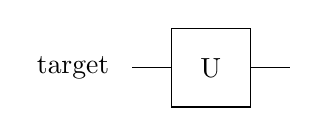
\begin{tikzpicture}[scale=.5] \node[draw=none] at (-3.5, 0) {target}; \draw (-2,0) -- (-1, 0); \draw (1, 0) -- (2, 0); \draw (-1,-1)--(-1,1)--(1,1)--(1,-1)--cycle; \node[draw=none] at (0, 0) {U}; \end{tikzpicture} } \]


\begin{DoxyParams}{Parameters}
\item[\mbox{$\leftrightarrow$} {\em multiQubit}]object representing the set of all qubits \item[\mbox{$\leftarrow$} {\em targetQubit}]qubit to operate on \item[\mbox{$\leftarrow$} {\em alpha}]complex unitary parameter (row 1, column 1) \item[\mbox{$\leftarrow$} {\em beta}]complex unitary parameter (row 2, column 1) \end{DoxyParams}

\begin{DoxyExceptions}{Exceptions}
\item[{\em exitWithError}]if {\ttfamily targetQubit} is outside \mbox{[}0, {\ttfamily multiQubit.numQubits}), or if {\ttfamily alpha}, {\ttfamily beta} don't satisfy $|${\ttfamily alpha$|$$^\wedge$2} + $|${\ttfamily beta$|$$^\wedge$2} = 1. \end{DoxyExceptions}


Definition at line 104 of file qubits\_\-env\_\-local.c.

References MultiQubit::chunkId, chunkIsUpper(), compactUnitaryDistributed(), compactUnitaryLocal(), exchangeStateVectors(), getChunkPairId(), getRotAngle(), halfMatrixBlockFitsInChunk(), MultiQubit::numAmps, MultiQubit::numQubits, MultiQubit::pairStateVec, QuESTAssert(), MultiQubit::stateVec, and validateAlphaBeta().

Referenced by rotateAroundAxis().


\begin{DoxyCode}
105 {
106     QuESTAssert(targetQubit >= 0 && targetQubit < multiQubit.numQubits, 1, __func
      __);
107     QuESTAssert(validateAlphaBeta(alpha, beta), 6, __func__);
108 
109         // all values required to update state vector lie in this rank
110         compactUnitaryLocal(multiQubit, targetQubit, alpha, beta);
111 }
\end{DoxyCode}
\hypertarget{qubits_8h_ab4812953bc457405b3aa05a4c2f64f4a}{
\index{qubits.h@{qubits.h}!controlledCompactUnitary@{controlledCompactUnitary}}
\index{controlledCompactUnitary@{controlledCompactUnitary}!qubits.h@{qubits.h}}
\paragraph[{controlledCompactUnitary}]{\setlength{\rightskip}{0pt plus 5cm}void controlledCompactUnitary ({\bf MultiQubit} {\em multiQubit}, \/  const int {\em controlQubit}, \/  const int {\em targetQubit}, \/  {\bf Complex} {\em alpha}, \/  {\bf Complex} {\em beta})}\hfill}
\label{qubits_8h_ab4812953bc457405b3aa05a4c2f64f4a}


Apply a controlled unitary (single control, single target) parameterised by two given complex scalars. Given valid complex numbers $\alpha$ and $\beta$, applies the two-\/qubit unitary \[ \begin{pmatrix} 1 \\ & 1 \\ & & \alpha & -\beta^* \\ & & \beta & \alpha^* \end{pmatrix} \] to the control and target qubits. Valid $\alpha$, $\beta$ satisfy $|\alpha|^2 + |\beta|^2 = 1$. The target unitary is general up to a global phase factor.

\[ \setlength{\fboxrule}{0.01pt} \fbox{ 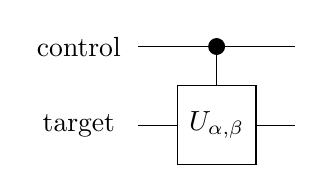
\begin{tikzpicture}[scale=.5] \node[draw=none] at (-3.5, 2) {control}; \node[draw=none] at (-3.5, 0) {target}; \draw (-2, 2) -- (2, 2); \draw[fill=black] (0, 2) circle (.2); \draw (0, 2) -- (0, 1); \draw (-2,0) -- (-1, 0); \draw (1, 0) -- (2, 0); \draw (-1,-1)--(-1,1)--(1,1)--(1,-1)--cycle; \node[draw=none] at (0, 0) {$U_{\alpha, \beta}$}; \end{tikzpicture} } \]


\begin{DoxyParams}{Parameters}
\item[\mbox{$\leftrightarrow$} {\em multiQubit}]object representing the set of all qubits \item[\mbox{$\leftarrow$} {\em controlQubit}]apply the target unitary if this qubit has value 1 \item[\mbox{$\leftarrow$} {\em targetQubit}]qubit on which to apply the target unitary \item[\mbox{$\leftarrow$} {\em alpha}]complex unitary parameter (row 1, column 1) \item[\mbox{$\leftarrow$} {\em beta}]complex unitary parameter (row 2, column 1) \end{DoxyParams}

\begin{DoxyExceptions}{Exceptions}
\item[{\em exitWithError}]if either {\ttfamily controlQubit} or {\ttfamily targetQubit} are outside \mbox{[}0, {\ttfamily multiQubit.numQubits}) or are equal, or if {\ttfamily alpha}, {\ttfamily beta} don't satisfy $|${\ttfamily alpha$|$$^\wedge$2} + $|${\ttfamily beta$|$$^\wedge$2} = 1. \end{DoxyExceptions}


Definition at line 122 of file qubits\_\-env\_\-local.c.

References MultiQubit::chunkId, chunkIsUpper(), controlledCompactUnitaryDistributed(), controlledCompactUnitaryLocal(), exchangeStateVectors(), getChunkPairId(), getRotAngle(), halfMatrixBlockFitsInChunk(), MultiQubit::numAmps, MultiQubit::numQubits, MultiQubit::pairStateVec, QuESTAssert(), MultiQubit::stateVec, and validateAlphaBeta().

Referenced by controlledRotateAroundAxis().


\begin{DoxyCode}
123 {
124     QuESTAssert(targetQubit >= 0 && targetQubit < multiQubit.numQubits, 1, __func
      __);
125     QuESTAssert(controlQubit >= 0 && controlQubit < multiQubit.numQubits, 2, __fu
      nc__);
126     QuESTAssert(controlQubit != targetQubit, 3, __func__);
127     QuESTAssert(validateAlphaBeta(alpha, beta), 6, __func__);
128     
129 
130         controlledCompactUnitaryLocal(multiQubit, controlQubit, targetQubit, alph
      a, beta);
131 }
\end{DoxyCode}
\hypertarget{qubits_8h_a67576895bbc65463481a8ea24d9b1e22}{
\index{qubits.h@{qubits.h}!controlledNot@{controlledNot}}
\index{controlledNot@{controlledNot}!qubits.h@{qubits.h}}
\paragraph[{controlledNot}]{\setlength{\rightskip}{0pt plus 5cm}void controlledNot ({\bf MultiQubit} {\em multiQubit}, \/  const int {\em controlQubit}, \/  const int {\em targetQubit})}\hfill}
\label{qubits_8h_a67576895bbc65463481a8ea24d9b1e22}


Apply the controlled not (single control, single target) gate, also known as the c-\/X, c-\/sigma-\/X, c-\/Pauli-\/X and c-\/bit-\/flip gate. This applies sigmaX to the target qubit if the control qubit has value 1. This effects the two-\/qubit unitary \[ \begin{pmatrix} 1 \\ & 1 \\\ & & & 1 \\ & & 1 \end{pmatrix} \] on the control and target qubits.

\[ \setlength{\fboxrule}{0.01pt} \fbox{ 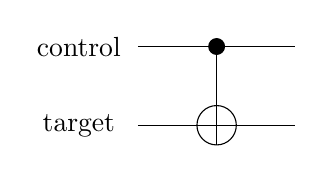
\begin{tikzpicture}[scale=.5] \node[draw=none] at (-3.5, 2) {control}; \node[draw=none] at (-3.5, 0) {target}; \draw (-2, 2) -- (2, 2); \draw[fill=black] (0, 2) circle (.2); \draw (0, 2) -- (0, -.5); \draw (-2,0) -- (2, 0); \draw (0, 0) circle (.5); \end{tikzpicture} } \]


\begin{DoxyParams}{Parameters}
\item[\mbox{$\leftrightarrow$} {\em multiQubit}]object representing the set of all qubits \item[\mbox{$\leftarrow$} {\em controlQubit}]nots the target if this qubit is 1 \item[\mbox{$\leftarrow$} {\em targetQubit}]qubit to not \end{DoxyParams}

\begin{DoxyExceptions}{Exceptions}
\item[{\em exitWithError}]if either {\ttfamily controlQubit} or {\ttfamily targetQubit} are outside \mbox{[}0, {\ttfamily multiQubit.numQubits}), or are equal. \end{DoxyExceptions}


Definition at line 181 of file qubits\_\-env\_\-local.c.

References MultiQubit::chunkId, chunkIsUpper(), controlledNotDistributed(), controlledNotLocal(), exchangeStateVectors(), getChunkPairId(), halfMatrixBlockFitsInChunk(), MultiQubit::numAmps, MultiQubit::numQubits, MultiQubit::pairStateVec, QuESTAssert(), and MultiQubit::stateVec.


\begin{DoxyCode}
182 {
183     QuESTAssert(targetQubit >= 0 && targetQubit < multiQubit.numQubits, 1, __func
      __);
184     QuESTAssert(controlQubit >= 0 && controlQubit < multiQubit.numQubits, 2, __fu
      nc__);
185     QuESTAssert(controlQubit != targetQubit, 3, __func__);
186         controlledNotLocal(multiQubit, controlQubit, targetQubit);
187 }
\end{DoxyCode}
\hypertarget{qubits_8h_a11a96159191cbf1b01a1080e7f045aac}{
\index{qubits.h@{qubits.h}!controlledPhaseGate@{controlledPhaseGate}}
\index{controlledPhaseGate@{controlledPhaseGate}!qubits.h@{qubits.h}}
\paragraph[{controlledPhaseGate}]{\setlength{\rightskip}{0pt plus 5cm}void controlledPhaseGate ({\bf MultiQubit} {\em multiQubit}, \/  const int {\em idQubit1}, \/  const int {\em idQubit2})}\hfill}
\label{qubits_8h_a11a96159191cbf1b01a1080e7f045aac}


Apply the (two-\/qubit) controlled phase gate, also known as the controlled sigmaZ gate. For each state, if both input qubits have value one, multiply the amplitude of that state by -\/1. This applies the two-\/qubit unitary: \[ \begin{pmatrix} 1 \\ & 1 \\\ & & 1 \\ & & & -1 \end{pmatrix} \]

\[ \setlength{\fboxrule}{0.01pt} \fbox{ 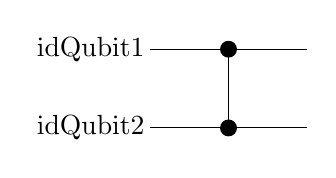
\begin{tikzpicture}[scale=.5] \node[draw=none] at (-3.5, 2) {idQubit1}; \node[draw=none] at (-3.5, 0) {idQubit2}; \draw (-2, 2) -- (2, 2); \draw[fill=black] (0, 2) circle (.2); \draw (0, 2) -- (0, 0); \draw (-2,0) -- (2, 0); \draw[fill=black] (0, 0) circle (.2); \end{tikzpicture} } \]


\begin{DoxyParams}{Parameters}
\item[\mbox{$\leftrightarrow$} {\em multiQubit}]object representing the set of all qubits \item[\mbox{$\leftarrow$} {\em idQubit1,idQubit2}]qubits to operate upon \end{DoxyParams}

\begin{DoxyExceptions}{Exceptions}
\item[{\em exitWithError}]if {\ttfamily idQubit1} or {\ttfamily idQubit2} are outside \mbox{[}0, {\ttfamily multiQubit.numQubits}), or are equal \end{DoxyExceptions}


Definition at line 1729 of file qubits.c.

References MultiQubit::chunkId, extractBit(), ComplexArray::imag, MultiQubit::numAmps, MultiQubit::numQubits, QuESTAssert(), ComplexArray::real, REAL, and MultiQubit::stateVec.


\begin{DoxyCode}
1730 {
1731         long long int index;
1732         long long int stateVecSize;
1733         int bit1, bit2;
1734 
1735         const long long int chunkSize=multiQubit.numAmps;
1736         const long long int chunkId=multiQubit.chunkId;
1737 
1738     QuESTAssert(idQubit1 >= 0 && idQubit1 < multiQubit.numQubits, 2, __func__);
1739     QuESTAssert(idQubit2 >= 0 && idQubit2 < multiQubit.numQubits, 1, __func__);
1740     QuESTAssert(idQubit1 != idQubit2, 3, __func__);
1741 
1742         // dimension of the state vector
1743         stateVecSize = multiQubit.numAmps;
1744         REAL *stateVecReal = multiQubit.stateVec.real;
1745         REAL *stateVecImag = multiQubit.stateVec.imag;
1746 
1747 # ifdef _OPENMP
1748 # pragma omp parallel for \
1749         default  (none)                      \
1750         shared   (stateVecSize, stateVecReal,stateVecImag ) \
1751         private  (index,bit1,bit2)                     \
1752         schedule (static)
1753 # endif
1754         for (index=0; index<stateVecSize; index++) {
1755                 bit1 = extractBit (idQubit1, index+chunkId*chunkSize);
1756                 bit2 = extractBit (idQubit2, index+chunkId*chunkSize);
1757                 if (bit1 && bit2) {
1758                         stateVecReal [index] = - stateVecReal [index];
1759                         stateVecImag [index] = - stateVecImag [index];
1760                 }
1761         }
1762 }
\end{DoxyCode}
\hypertarget{qubits_8h_ad41f82b41149393a642391b67b3a287e}{
\index{qubits.h@{qubits.h}!controlledRotateAroundAxis@{controlledRotateAroundAxis}}
\index{controlledRotateAroundAxis@{controlledRotateAroundAxis}!qubits.h@{qubits.h}}
\paragraph[{controlledRotateAroundAxis}]{\setlength{\rightskip}{0pt plus 5cm}void controlledRotateAroundAxis ({\bf MultiQubit} {\em multiQubit}, \/  const int {\em controlQubit}, \/  const int {\em targetQubit}, \/  REAL {\em angle}, \/  {\bf Vector} {\em axis})}\hfill}
\label{qubits_8h_ad41f82b41149393a642391b67b3a287e}


Applies a controlled rotation by a given angle around a given vector on the Bloch-\/sphere. The vector must not be zero (else an error is thrown), but needn't be unit magnitude.

For angle $\theta$ and axis vector $\vec{n}$, applies $R_{\hat{n}} = \exp \left(- i \frac{\theta}{2} \hat{n} \cdot \vec{\sigma} \right) $ to states where the target qubit is 1 ($\vec{\sigma}$ is the vector of Pauli matrices).

\[ \setlength{\fboxrule}{0.01pt} \fbox{ 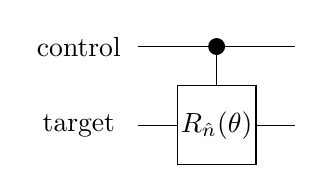
\begin{tikzpicture}[scale=.5] \node[draw=none] at (-3.5, 2) {control}; \node[draw=none] at (-3.5, 0) {target}; \draw (-2, 2) -- (2, 2); \draw[fill=black] (0, 2) circle (.2); \draw (0, 2) -- (0, 1); \draw (-2,0) -- (-1, 0); \draw (1, 0) -- (2, 0); \draw (-1,-1)--(-1,1)--(1,1)--(1,-1)--cycle; \node[draw=none] at (0, 0) {$R_{\hat{n}}(\theta)$}; \end{tikzpicture} } \]


\begin{DoxyParams}{Parameters}
\item[\mbox{$\leftrightarrow$} {\em multiQubit}]object representing the set of all qubits \item[\mbox{$\leftarrow$} {\em controlQubit}]qubit with value 1 in the rotated states \item[\mbox{$\leftarrow$} {\em targetQubit}]qubit to rotate \item[\mbox{$\leftarrow$} {\em angle}]angle by which to rotate in radians \item[\mbox{$\leftarrow$} {\em axis}]vector around which to rotate (can be non-\/unit; will be normalised) \end{DoxyParams}

\begin{DoxyExceptions}{Exceptions}
\item[{\em exitWithError}]if either {\ttfamily controlQubit} or {\ttfamily targetQubit} are outside \mbox{[}0, {\ttfamily multiQubit.numQubits}) or are equal or if {\ttfamily axis} is the zero vector \end{DoxyExceptions}


Definition at line 682 of file qubits.h.

References controlledCompactUnitary(), Complex::imag, Complex::real, Vector::x, Vector::y, and Vector::z.


\begin{DoxyCode}
682                                                                                  
                                                   {
683         
684         double mag = sqrt(pow(axis.x,2) + pow(axis.y,2) + pow(axis.z,2));
685         Vector unitAxis = {axis.x/mag, axis.y/mag, axis.z/mag};
686         
687         Complex alpha, beta;
688         alpha.real = cos(angle/2.0);
689         alpha.imag = -sin(angle/2.0)*unitAxis.z;        
690         beta.real = sin(angle/2.0)*unitAxis.y;
691         beta.imag = -sin(angle/2.0)*unitAxis.x;
692         controlledCompactUnitary(multiQubit, controlQubit, targetQubit, alpha, be
      ta);
693 }
\end{DoxyCode}
\hypertarget{qubits_8h_ac6923ac57e67d9a21096e06f6a9012f6}{
\index{qubits.h@{qubits.h}!controlledRotateX@{controlledRotateX}}
\index{controlledRotateX@{controlledRotateX}!qubits.h@{qubits.h}}
\paragraph[{controlledRotateX}]{\setlength{\rightskip}{0pt plus 5cm}void controlledRotateX ({\bf MultiQubit} {\em multiQubit}, \/  const int {\em controlQubit}, \/  const int {\em targetQubit}, \/  REAL {\em angle})}\hfill}
\label{qubits_8h_ac6923ac57e67d9a21096e06f6a9012f6}


Applies a controlled rotation by a given angle around the X-\/axis of the Bloch-\/sphere. The target qubit is rotated in states where the control qubit has value 1.

\[ \setlength{\fboxrule}{0.01pt} \fbox{ 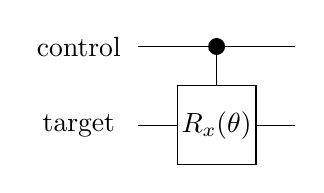
\begin{tikzpicture}[scale=.5] \node[draw=none] at (-3.5, 2) {control}; \node[draw=none] at (-3.5, 0) {target}; \draw (-2, 2) -- (2, 2); \draw[fill=black] (0, 2) circle (.2); \draw (0, 2) -- (0, 1); \draw (-2,0) -- (-1, 0); \draw (1, 0) -- (2, 0); \draw (-1,-1)--(-1,1)--(1,1)--(1,-1)--cycle; \node[draw=none] at (0, 0) {$R_x(\theta)$}; \end{tikzpicture} } \]


\begin{DoxyParams}{Parameters}
\item[\mbox{$\leftrightarrow$} {\em multiQubit}]object representing the set of all qubits \item[\mbox{$\leftarrow$} {\em controlQubit}]qubit which has value 1 in the rotated states \item[\mbox{$\leftarrow$} {\em tagretQubit}]qubit to rotate \item[\mbox{$\leftarrow$} {\em angle}]angle by which to rotate the target qubit in radians \end{DoxyParams}

\begin{DoxyExceptions}{Exceptions}
\item[{\em exitWithError}]if either {\ttfamily controlQubit} or {\ttfamily targetQubit} are outside \mbox{[}0, {\ttfamily multiQubit.numQubits}) or are equal. \end{DoxyExceptions}


Definition at line 572 of file qubits.h.

References controlledRotateAroundAxis().


\begin{DoxyCode}
572                                                                                  
                             {
573 
574         Vector unitAxis = {1, 0, 0};
575         controlledRotateAroundAxis(multiQubit, controlQubit, targetQubit, angle, 
      unitAxis);
576 }
\end{DoxyCode}
\hypertarget{qubits_8h_a71e90a2f7292116338c062934f9d1202}{
\index{qubits.h@{qubits.h}!controlledRotateY@{controlledRotateY}}
\index{controlledRotateY@{controlledRotateY}!qubits.h@{qubits.h}}
\paragraph[{controlledRotateY}]{\setlength{\rightskip}{0pt plus 5cm}void controlledRotateY ({\bf MultiQubit} {\em multiQubit}, \/  const int {\em controlQubit}, \/  const int {\em targetQubit}, \/  REAL {\em angle})}\hfill}
\label{qubits_8h_a71e90a2f7292116338c062934f9d1202}


Applies a controlled rotation by a given angle around the Y-\/axis of the Bloch-\/sphere. The target qubit is rotated in states where the control qubit has value 1.

\[ \setlength{\fboxrule}{0.01pt} \fbox{ 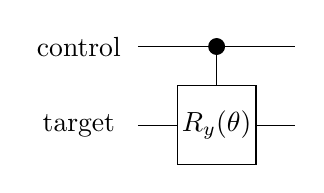
\begin{tikzpicture}[scale=.5] \node[draw=none] at (-3.5, 2) {control}; \node[draw=none] at (-3.5, 0) {target}; \draw (-2, 2) -- (2, 2); \draw[fill=black] (0, 2) circle (.2); \draw (0, 2) -- (0, 1); \draw (-2,0) -- (-1, 0); \draw (1, 0) -- (2, 0); \draw (-1,-1)--(-1,1)--(1,1)--(1,-1)--cycle; \node[draw=none] at (0, 0) {$R_y(\theta)$}; \end{tikzpicture} } \]


\begin{DoxyParams}{Parameters}
\item[\mbox{$\leftrightarrow$} {\em multiQubit}]object representing the set of all qubits \item[\mbox{$\leftarrow$} {\em controlQubit}]qubit which has value 1 in the rotated states \item[\mbox{$\leftarrow$} {\em tagretQubit}]qubit to rotate \item[\mbox{$\leftarrow$} {\em angle}]angle by which to rotate the target qubit in radians \end{DoxyParams}

\begin{DoxyExceptions}{Exceptions}
\item[{\em exitWithError}]if either {\ttfamily controlQubit} or {\ttfamily targetQubit} are outside \mbox{[}0, {\ttfamily multiQubit.numQubits}) or are equal. \end{DoxyExceptions}


Definition at line 607 of file qubits.h.

References controlledRotateAroundAxis().


\begin{DoxyCode}
607                                                                                  
                             {
608 
609         Vector unitAxis = {0, 1, 0};
610         controlledRotateAroundAxis(multiQubit, controlQubit, targetQubit, angle, 
      unitAxis);
611 }
\end{DoxyCode}
\hypertarget{qubits_8h_a668e5d2634b02e98bc73675ccb11d61c}{
\index{qubits.h@{qubits.h}!controlledRotateZ@{controlledRotateZ}}
\index{controlledRotateZ@{controlledRotateZ}!qubits.h@{qubits.h}}
\paragraph[{controlledRotateZ}]{\setlength{\rightskip}{0pt plus 5cm}void controlledRotateZ ({\bf MultiQubit} {\em multiQubit}, \/  const int {\em controlQubit}, \/  const int {\em targetQubit}, \/  REAL {\em angle})}\hfill}
\label{qubits_8h_a668e5d2634b02e98bc73675ccb11d61c}


Applies a controlled rotation by a given angle around the Z-\/axis of the Bloch-\/sphere. The target qubit is rotated in states where the control qubit has value 1.

\[ \setlength{\fboxrule}{0.01pt} \fbox{ 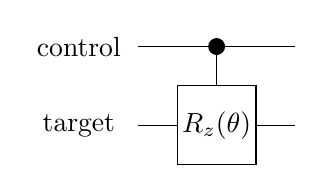
\begin{tikzpicture}[scale=.5] \node[draw=none] at (-3.5, 2) {control}; \node[draw=none] at (-3.5, 0) {target}; \draw (-2, 2) -- (2, 2); \draw[fill=black] (0, 2) circle (.2); \draw (0, 2) -- (0, 1); \draw (-2,0) -- (-1, 0); \draw (1, 0) -- (2, 0); \draw (-1,-1)--(-1,1)--(1,1)--(1,-1)--cycle; \node[draw=none] at (0, 0) {$R_z(\theta)$}; \end{tikzpicture} } \]


\begin{DoxyParams}{Parameters}
\item[\mbox{$\leftrightarrow$} {\em multiQubit}]object representing the set of all qubits \item[\mbox{$\leftarrow$} {\em controlQubit}]qubit which has value 1 in the rotated states \item[\mbox{$\leftarrow$} {\em tagretQubit}]qubit to rotate \item[\mbox{$\leftarrow$} {\em angle}]angle by which to rotate the target qubit in radians \end{DoxyParams}

\begin{DoxyExceptions}{Exceptions}
\item[{\em exitWithError}]if either {\ttfamily controlQubit} or {\ttfamily targetQubit} are outside \mbox{[}0, {\ttfamily multiQubit.numQubits}) or are equal. \end{DoxyExceptions}


Definition at line 642 of file qubits.h.

References controlledRotateAroundAxis().


\begin{DoxyCode}
642                                                                                  
                             {
643 
644         Vector unitAxis = {0, 0, 1};
645         controlledRotateAroundAxis(multiQubit, controlQubit, targetQubit, angle, 
      unitAxis);
646 }
\end{DoxyCode}
\hypertarget{qubits_8h_a8a701526263392599aa21d0d0f05d9d8}{
\index{qubits.h@{qubits.h}!controlledUnitary@{controlledUnitary}}
\index{controlledUnitary@{controlledUnitary}!qubits.h@{qubits.h}}
\paragraph[{controlledUnitary}]{\setlength{\rightskip}{0pt plus 5cm}void controlledUnitary ({\bf MultiQubit} {\em multiQubit}, \/  const int {\em controlQubit}, \/  const int {\em targetQubit}, \/  {\bf ComplexMatrix2} {\em u})}\hfill}
\label{qubits_8h_a8a701526263392599aa21d0d0f05d9d8}


Apply a general controlled unitary (single control, single target), which can include a global phase factor. The given unitary is applied to the target qubit if the control qubit has value 1, effecting the two-\/qubit unitary \[ \begin{pmatrix} 1 \\ & 1 \\ & & u_{00} & u_{01}\\ & & u_{10} & u_{11} \end{pmatrix} \] on the control and target qubits.

\[ \setlength{\fboxrule}{0.01pt} \fbox{ 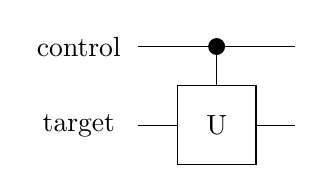
\begin{tikzpicture}[scale=.5] \node[draw=none] at (-3.5, 2) {control}; \node[draw=none] at (-3.5, 0) {target}; \draw (-2, 2) -- (2, 2); \draw[fill=black] (0, 2) circle (.2); \draw (0, 2) -- (0, 1); \draw (-2,0) -- (-1, 0); \draw (1, 0) -- (2, 0); \draw (-1,-1)--(-1,1)--(1,1)--(1,-1)--cycle; \node[draw=none] at (0, 0) {U}; \end{tikzpicture} } \]


\begin{DoxyParams}{Parameters}
\item[\mbox{$\leftrightarrow$} {\em multiQubit}]object representing the set of all qubits \item[\mbox{$\leftarrow$} {\em controlQubit}]apply unitary if this qubit is 1 \item[\mbox{$\leftarrow$} {\em targetQubit}]qubit to operate on \item[\mbox{$\leftarrow$} {\em u}]single-\/qubit unitary matrix to apply \end{DoxyParams}

\begin{DoxyExceptions}{Exceptions}
\item[{\em exitWithError}]if either {\ttfamily controlQubit} or {\ttfamily targetQubit} are outside \mbox{[}0, {\ttfamily multiQubit.numQubits}) or are equal, or if {\ttfamily u} is not unitary. \end{DoxyExceptions}


Definition at line 133 of file qubits\_\-env\_\-local.c.

References MultiQubit::chunkId, chunkIsUpper(), controlledUnitaryDistributed(), controlledUnitaryLocal(), exchangeStateVectors(), getChunkPairId(), getRotAngleFromUnitaryMatrix(), halfMatrixBlockFitsInChunk(), MultiQubit::numAmps, MultiQubit::numQubits, MultiQubit::pairStateVec, QuESTAssert(), MultiQubit::stateVec, and validateMatrixIsUnitary().


\begin{DoxyCode}
134 {
135     QuESTAssert(targetQubit >= 0 && targetQubit < multiQubit.numQubits, 1, __func
      __);
136     QuESTAssert(controlQubit >= 0 && controlQubit < multiQubit.numQubits, 2, __fu
      nc__);
137     QuESTAssert(controlQubit != targetQubit, 3, __func__);
138     QuESTAssert(validateMatrixIsUnitary(u), 5, __func__);
139    
140         controlledUnitaryLocal(multiQubit, controlQubit, targetQubit, u);
141 }
\end{DoxyCode}
\hypertarget{qubits_8h_a9c02591bc64c2918503afa231d90d83f}{
\index{qubits.h@{qubits.h}!createMultiQubit@{createMultiQubit}}
\index{createMultiQubit@{createMultiQubit}!qubits.h@{qubits.h}}
\paragraph[{createMultiQubit}]{\setlength{\rightskip}{0pt plus 5cm}void createMultiQubit ({\bf MultiQubit} $\ast$ {\em multiQubit}, \/  int {\em numQubits}, \/  {\bf QuESTEnv} {\em env})}\hfill}
\label{qubits_8h_a9c02591bc64c2918503afa231d90d83f}


Create a \hyperlink{structMultiQubit}{MultiQubit} object representing a set of qubits. Allocate space for state vector of probability amplitudes, including space for temporary values to be copied from one other chunk if running the distributed version. Define properties related to the size of the set of qubits. initStateZero should be called after this to initialise the qubits to the zero state.


\begin{DoxyParams}{Parameters}
\item[\mbox{$\leftrightarrow$} {\em multiQubit}]a pointer to an object representing the set of qubits \item[\mbox{$\leftarrow$} {\em numQubits}]number of qubits in the system \item[\mbox{$\leftarrow$} {\em env}]object representing the execution environment (local, multinode etc) \end{DoxyParams}

\begin{DoxyExceptions}{Exceptions}
\item[{\em exitWithError}]if {\ttfamily numQubits} $<$= 0 \end{DoxyExceptions}


Definition at line 39 of file qubits.c.

References MultiQubit::chunkId, ComplexArray::imag, MultiQubit::numAmps, MultiQubit::numChunks, MultiQubit::numQubits, QuESTEnv::numRanks, MultiQubit::pairStateVec, QuESTAssert(), QuESTEnv::rank, ComplexArray::real, and MultiQubit::stateVec.


\begin{DoxyCode}
40 {
41     QuESTAssert(numQubits>0, 9, __func__);
42         long long int numAmps = 1L << numQubits;
43         long long int numAmpsPerRank = numAmps/env.numRanks;
44 
45         multiQubit->stateVec.real = malloc(numAmpsPerRank * sizeof(*(multiQubit->
      stateVec.real)));
46         multiQubit->stateVec.imag = malloc(numAmpsPerRank * sizeof(*(multiQubit->
      stateVec.imag)));
47         if (env.numRanks>1){
48                 multiQubit->pairStateVec.real = malloc(numAmpsPerRank * sizeof(*(
      multiQubit->pairStateVec.real)));
49                 multiQubit->pairStateVec.imag = malloc(numAmpsPerRank * sizeof(*(
      multiQubit->pairStateVec.imag)));
50         }
51 
52         if ( (!(multiQubit->stateVec.real) || !(multiQubit->stateVec.imag))
53                  && numAmpsPerRank ) {
54                 printf("Could not allocate memory!");
55                 exit (EXIT_FAILURE);
56         }
57 
58         if ( env.numRanks>1 && (!(multiQubit->pairStateVec.real) || !(multiQubit-
      >pairStateVec.imag))
59                  && numAmpsPerRank ) {
60                 printf("Could not allocate memory!");
61                 exit (EXIT_FAILURE);
62         }
63 
64         multiQubit->numQubits = numQubits;
65         multiQubit->numAmps = numAmpsPerRank;
66         multiQubit->chunkId = env.rank;
67         multiQubit->numChunks = env.numRanks;
68 
69 }
\end{DoxyCode}
\hypertarget{qubits_8h_ae5d6acc322314d7a3d8a2eccf00d3b19}{
\index{qubits.h@{qubits.h}!destroyMultiQubit@{destroyMultiQubit}}
\index{destroyMultiQubit@{destroyMultiQubit}!qubits.h@{qubits.h}}
\paragraph[{destroyMultiQubit}]{\setlength{\rightskip}{0pt plus 5cm}void destroyMultiQubit ({\bf MultiQubit} {\em multiQubit}, \/  {\bf QuESTEnv} {\em env})}\hfill}
\label{qubits_8h_ae5d6acc322314d7a3d8a2eccf00d3b19}


Deallocate a \hyperlink{structMultiQubit}{MultiQubit} object representing a set of qubits. Free memory allocated to state vector of probability amplitudes, including temporary vector for values copied from another chunk if running the distributed version.


\begin{DoxyParams}{Parameters}
\item[\mbox{$\leftrightarrow$} {\em multiQubit}]object to be deallocated \item[\mbox{$\leftarrow$} {\em env}]object representing the execution environment (local, multinode etc) \end{DoxyParams}


Definition at line 71 of file qubits.c.

References ComplexArray::imag, QuESTEnv::numRanks, MultiQubit::pairStateVec, ComplexArray::real, and MultiQubit::stateVec.


\begin{DoxyCode}
71                                                            {
72         free(multiQubit.stateVec.real);
73         free(multiQubit.stateVec.imag);
74         if (env.numRanks>1){
75                 free(multiQubit.pairStateVec.real);
76                 free(multiQubit.pairStateVec.imag);
77         }
78 }
\end{DoxyCode}
\hypertarget{qubits_8h_ad315c941a51bc053d39ebfa2040fd32e}{
\index{qubits.h@{qubits.h}!findProbabilityOfOutcome@{findProbabilityOfOutcome}}
\index{findProbabilityOfOutcome@{findProbabilityOfOutcome}!qubits.h@{qubits.h}}
\paragraph[{findProbabilityOfOutcome}]{\setlength{\rightskip}{0pt plus 5cm}REAL findProbabilityOfOutcome ({\bf MultiQubit} {\em multiQubit}, \/  const int {\em measureQubit}, \/  int {\em outcome})}\hfill}
\label{qubits_8h_ad315c941a51bc053d39ebfa2040fd32e}


Gives the probability of a specified qubit being measured in the given outcome (0 or 1). This performs no actual measurement and does not change the state of the qubits.


\begin{DoxyParams}{Parameters}
\item[\mbox{$\leftarrow$} {\em multiQubit}]object representing the set of all qubits \item[\mbox{$\leftarrow$} {\em measureQubit}]qubit to study \item[\mbox{$\leftarrow$} {\em outcome}]for which to find the probability of the qubit being measured in \end{DoxyParams}
\begin{DoxyReturn}{Returns}
probability of qubit measureQubit being measured in the given outcome 
\end{DoxyReturn}

\begin{DoxyExceptions}{Exceptions}
\item[{\em exitWithError}]if {\ttfamily measureQubit} is outside \mbox{[}0, {\ttfamily multiQubit.numQubits}), or if {\ttfamily outcome} is not in \{0, 1\}. \end{DoxyExceptions}


Definition at line 189 of file qubits\_\-env\_\-local.c.

References MultiQubit::chunkId, findProbabilityOfZeroDistributed(), findProbabilityOfZeroLocal(), halfMatrixBlockFitsInChunk(), isChunkToSkipInFindPZero(), MPI\_\-QuEST\_\-REAL, MultiQubit::numAmps, MultiQubit::numQubits, QuESTAssert(), and REAL.

Referenced by collapseToOutcome(), and measureWithStats().


\begin{DoxyCode}
190 {
191     QuESTAssert(measureQubit >= 0 && measureQubit < multiQubit.numQubits, 2, __fu
      nc__);
192         REAL stateProb=0;
193         stateProb = findProbabilityOfZeroLocal(multiQubit, measureQubit);
194         if (outcome==1) stateProb = 1.0 - stateProb;
195         return stateProb;
196 }
\end{DoxyCode}
\hypertarget{qubits_8h_a8f10aabf9f607f19093aee54630caa21}{
\index{qubits.h@{qubits.h}!getEnvironmentString@{getEnvironmentString}}
\index{getEnvironmentString@{getEnvironmentString}!qubits.h@{qubits.h}}
\paragraph[{getEnvironmentString}]{\setlength{\rightskip}{0pt plus 5cm}void getEnvironmentString ({\bf QuESTEnv} {\em env}, \/  {\bf MultiQubit} {\em multiQubit}, \/  char {\em str}\mbox{[}200\mbox{]})}\hfill}
\label{qubits_8h_a8f10aabf9f607f19093aee54630caa21}


Definition at line 131 of file qubits.c.

References MultiQubit::numQubits, and QuESTEnv::numRanks.


\begin{DoxyCode}
131                                                                              {
132         int numThreads=1;
133 # ifdef _OPENMP
134         numThreads=omp_get_max_threads(); 
135 # endif
136         sprintf(str, "%dqubits_CPU_%dranksx%dthreads", multiQubit.numQubits, env.
      numRanks, numThreads);
137 }
\end{DoxyCode}
\hypertarget{qubits_8h_a3615f76fd5f57008d9b74bbd10533dd0}{
\index{qubits.h@{qubits.h}!getImagAmpEl@{getImagAmpEl}}
\index{getImagAmpEl@{getImagAmpEl}!qubits.h@{qubits.h}}
\paragraph[{getImagAmpEl}]{\setlength{\rightskip}{0pt plus 5cm}REAL getImagAmpEl ({\bf MultiQubit} {\em multiQubit}, \/  long long int {\em index})}\hfill}
\label{qubits_8h_a3615f76fd5f57008d9b74bbd10533dd0}


Get the imaginary component of the complex probability amplitude at an index in the state vector. For debugging purposes.


\begin{DoxyParams}{Parameters}
\item[\mbox{$\leftarrow$} {\em multiQubit}]object representing a set of qubits \item[\mbox{$\leftarrow$} {\em index}]index in state vector of probability amplitudes \end{DoxyParams}
\begin{DoxyReturn}{Returns}
imaginary component at that index 
\end{DoxyReturn}

\begin{DoxyExceptions}{Exceptions}
\item[{\em exitWithError}]if {\ttfamily index} is outside \mbox{[}0, $2^{N}$) where $N = $ {\ttfamily multiQubit.numQubits} \end{DoxyExceptions}


Definition at line 100 of file qubits\_\-env\_\-local.c.

References MultiQubit::chunkId, getChunkIdFromIndex(), ComplexArray::imag, MPI\_\-QuEST\_\-REAL, MultiQubit::numAmps, REAL, and MultiQubit::stateVec.

Referenced by getProbEl().


\begin{DoxyCode}
100                                                              {
101         return multiQubit.stateVec.imag[index];
102 }
\end{DoxyCode}
\hypertarget{qubits_8h_a799b10447d6dbdaf960a4d3eedd22014}{
\index{qubits.h@{qubits.h}!getProbEl@{getProbEl}}
\index{getProbEl@{getProbEl}!qubits.h@{qubits.h}}
\paragraph[{getProbEl}]{\setlength{\rightskip}{0pt plus 5cm}REAL getProbEl ({\bf MultiQubit} {\em multiQubit}, \/  long long int {\em index})}\hfill}
\label{qubits_8h_a799b10447d6dbdaf960a4d3eedd22014}


Get the probability of the state at an index in the full state vector. 
\begin{DoxyParams}{Parameters}
\item[\mbox{$\leftarrow$} {\em multiQubit}]object representing a set of qubits \item[\mbox{$\leftarrow$} {\em index}]index in state vector of probability amplitudes \end{DoxyParams}
\begin{DoxyReturn}{Returns}
realEl$\ast$realEl + imagEl$\ast$imagEl 
\end{DoxyReturn}

\begin{DoxyExceptions}{Exceptions}
\item[{\em exitWithError}]if {\ttfamily index} is outside \mbox{[}0, $2^{N}$) where $N = $ {\ttfamily multiQubit.numQubits} \end{DoxyExceptions}


Definition at line 1971 of file qubits.c.

References getImagAmpEl(), getRealAmpEl(), and REAL.


\begin{DoxyCode}
1971                                                           {
1972         REAL real;
1973         REAL imag;
1974         real = getRealAmpEl(multiQubit, index);
1975         imag = getImagAmpEl(multiQubit, index);
1976         return real*real + imag*imag;
1977 }
\end{DoxyCode}
\hypertarget{qubits_8h_a317b786f577fa6bc136ea7f0ee7330a7}{
\index{qubits.h@{qubits.h}!getRealAmpEl@{getRealAmpEl}}
\index{getRealAmpEl@{getRealAmpEl}!qubits.h@{qubits.h}}
\paragraph[{getRealAmpEl}]{\setlength{\rightskip}{0pt plus 5cm}REAL getRealAmpEl ({\bf MultiQubit} {\em multiQubit}, \/  long long int {\em index})}\hfill}
\label{qubits_8h_a317b786f577fa6bc136ea7f0ee7330a7}


Get the real component of the complex probability amplitude at an index in the state vector. For debugging purposes.


\begin{DoxyParams}{Parameters}
\item[\mbox{$\leftarrow$} {\em multiQubit}]object representing a set of qubits \item[\mbox{$\leftarrow$} {\em index}]index in state vector of probability amplitudes \end{DoxyParams}
\begin{DoxyReturn}{Returns}
real component at that index 
\end{DoxyReturn}

\begin{DoxyExceptions}{Exceptions}
\item[{\em exitWithError}]if {\ttfamily index} is outside \mbox{[}0, $2^{N}$) where $N = $ {\ttfamily multiQubit.numQubits} \end{DoxyExceptions}


Definition at line 96 of file qubits\_\-env\_\-local.c.

References MultiQubit::chunkId, getChunkIdFromIndex(), MPI\_\-QuEST\_\-REAL, MultiQubit::numAmps, REAL, ComplexArray::real, and MultiQubit::stateVec.

Referenced by getProbEl().


\begin{DoxyCode}
96                                                              {
97         return multiQubit.stateVec.real[index];
98 }
\end{DoxyCode}
\hypertarget{qubits_8h_aa09b5dd93de6df1384b8f2c0041749ab}{
\index{qubits.h@{qubits.h}!hadamard@{hadamard}}
\index{hadamard@{hadamard}!qubits.h@{qubits.h}}
\paragraph[{hadamard}]{\setlength{\rightskip}{0pt plus 5cm}void hadamard ({\bf MultiQubit} {\em multiQubit}, \/  const int {\em targetQubit})}\hfill}
\label{qubits_8h_aa09b5dd93de6df1384b8f2c0041749ab}


Apply the single-\/qubit Hadamard gate. This takes $|0\rangle$ to $|+\rangle$ and $|1\rangle$ to $|-\rangle$, and is equivalent to a rotation of $\pi$ around the x-\/axis then $\pi/2$ about the y-\/axis on the Bloch-\/sphere. I.e. \[ \frac{1}{\sqrt{2}} \begin{pmatrix} 1 & 1 \\ 1 & -1 \end{pmatrix} \]

\[ \setlength{\fboxrule}{0.01pt} \fbox{ 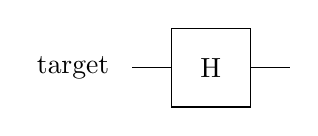
\begin{tikzpicture}[scale=.5] \node[draw=none] at (-3.5, 0) {target}; \draw (-2,0) -- (-1, 0); \draw (1, 0) -- (2, 0); \draw (-1,-1)--(-1,1)--(1,1)--(1,-1)--cycle; \node[draw=none] at (0, 0) {H}; \end{tikzpicture} } \]


\begin{DoxyParams}{Parameters}
\item[\mbox{$\leftrightarrow$} {\em multiQubit}]object representing the set of all qubits \item[\mbox{$\leftarrow$} {\em targetQubit}]qubit to operate on \end{DoxyParams}

\begin{DoxyExceptions}{Exceptions}
\item[{\em exitWithError}]if {\ttfamily targetQubit} is outside \mbox{[}0, {\ttfamily multiQubit.numQubits}). \end{DoxyExceptions}


Definition at line 175 of file qubits\_\-env\_\-local.c.

References MultiQubit::chunkId, chunkIsUpper(), exchangeStateVectors(), getChunkPairId(), hadamardDistributed(), hadamardLocal(), halfMatrixBlockFitsInChunk(), MultiQubit::numAmps, MultiQubit::numQubits, MultiQubit::pairStateVec, QuESTAssert(), and MultiQubit::stateVec.


\begin{DoxyCode}
176 {
177     QuESTAssert(targetQubit >= 0 && targetQubit < multiQubit.numQubits, 1, __func
      __);
178         hadamardLocal(multiQubit, targetQubit);
179 }
\end{DoxyCode}
\hypertarget{qubits_8h_ad84a3ce68d1ca02b4e3f741ea45b6054}{
\index{qubits.h@{qubits.h}!initQuESTEnv@{initQuESTEnv}}
\index{initQuESTEnv@{initQuESTEnv}!qubits.h@{qubits.h}}
\paragraph[{initQuESTEnv}]{\setlength{\rightskip}{0pt plus 5cm}void initQuESTEnv ({\bf QuESTEnv} $\ast$ {\em env})}\hfill}
\label{qubits_8h_ad84a3ce68d1ca02b4e3f741ea45b6054}


Initialize the QuEST environment. If something needs to be done to set up the execution environment, such as initializing MPI when running in distributed mode, it is handled here


\begin{DoxyParams}{Parameters}
\item[\mbox{$\leftrightarrow$} {\em env}]object representing the execution environment. A single instance is used for each program \end{DoxyParams}


Definition at line 22 of file qubits\_\-env\_\-local.c.

References DEBUG, init\_\-by\_\-array(), QuESTEnv::numRanks, and QuESTEnv::rank.


\begin{DoxyCode}
22                                 {
23         // init MPI environment
24         env->rank=0;
25         env->numRanks=1;
26 
27     // init MT random number generator with two keys -- time and pid
28     unsigned long int secs = time(NULL);
29     unsigned long int pid = getpid();
30     unsigned long int key[2];
31     key[0] = secs; key[1] = pid;
32     init_by_array(key, 2);
33 }
\end{DoxyCode}
\hypertarget{qubits_8h_a43bcb279fc9717fbd06a19cdef48b9d8}{
\index{qubits.h@{qubits.h}!initStatePlus@{initStatePlus}}
\index{initStatePlus@{initStatePlus}!qubits.h@{qubits.h}}
\paragraph[{initStatePlus}]{\setlength{\rightskip}{0pt plus 5cm}void initStatePlus ({\bf MultiQubit} $\ast$ {\em multiQubit})}\hfill}
\label{qubits_8h_a43bcb279fc9717fbd06a19cdef48b9d8}


Initialise a set of $ N $ qubits to the plus state $ {| + \rangle}^{\otimes N} = \frac{1}{\sqrt{2^N}} (| 0 \rangle + | 1 \rangle)^{\otimes N} $. This is the product state of $N$ qubits where every classical state is uniformly populated with real coefficient $\frac{1}{\sqrt{2^N}}$. This is equivalent to applying a Hadamard to every qubit in the zero state: $ \hat{H}^{\otimes N} {|0\rangle}^{\otimes N} $


\begin{DoxyParams}{Parameters}
\item[\mbox{$\leftrightarrow$} {\em multiQubit}]a pointer to the object representing the set of qubits to be initialised \end{DoxyParams}


Definition at line 177 of file qubits.c.

References DEBUG, ComplexArray::imag, MultiQubit::numAmps, MultiQubit::numChunks, ComplexArray::real, REAL, and MultiQubit::stateVec.


\begin{DoxyCode}
178 {
179         long long int chunkSize, stateVecSize;
180         long long int index;
181 
182         // dimension of the state vector
183         chunkSize = multiQubit->numAmps;
184         stateVecSize = chunkSize*multiQubit->numChunks;
185         REAL normFactor = 1.0/sqrt((REAL)stateVecSize);
186 
187         // Can't use multiQubit->stateVec as a private OMP var
188         REAL *stateVecReal = multiQubit->stateVec.real;
189         REAL *stateVecImag = multiQubit->stateVec.imag;
190 
191         // initialise the state to |0000..0000>
192 # ifdef _OPENMP
193 # pragma omp parallel \
194         default  (none) \
195         shared   (chunkSize, stateVecReal, stateVecImag, normFactor) \
196         private  (index) 
197 # endif
198         {
199 # ifdef _OPENMP
200                 # pragma omp for schedule (static)
201 # endif
202                 for (index=0; index<chunkSize; index++) {
203                         stateVecReal[index] = normFactor;
204                         stateVecImag[index] = 0.0;
205                 }
206         }
207         if (DEBUG) printf("COMPLETED INIT\n");
208 }
\end{DoxyCode}
\hypertarget{qubits_8h_acb5b2eff794339090004d29f02a70d9a}{
\index{qubits.h@{qubits.h}!initStateZero@{initStateZero}}
\index{initStateZero@{initStateZero}!qubits.h@{qubits.h}}
\paragraph[{initStateZero}]{\setlength{\rightskip}{0pt plus 5cm}void initStateZero ({\bf MultiQubit} $\ast$ {\em multiQubit})}\hfill}
\label{qubits_8h_acb5b2eff794339090004d29f02a70d9a}


Initialise a set of $ N $ qubits to the classical zero state $ {| 0 \rangle}^{\otimes N} $. 
\begin{DoxyParams}{Parameters}
\item[\mbox{$\leftrightarrow$} {\em multiQubit}]a pointer to the object representing the set of all qubits to initialise \end{DoxyParams}


Definition at line 139 of file qubits.c.

References MultiQubit::chunkId, DEBUG, ComplexArray::imag, MultiQubit::numAmps, ComplexArray::real, REAL, and MultiQubit::stateVec.


\begin{DoxyCode}
140 {
141         long long int stateVecSize;
142         long long int index;
143 
144         // dimension of the state vector
145         stateVecSize = multiQubit->numAmps;
146 
147         // Can't use multiQubit->stateVec as a private OMP var
148         REAL *stateVecReal = multiQubit->stateVec.real;
149         REAL *stateVecImag = multiQubit->stateVec.imag;
150 
151         // initialise the state to |0000..0000>
152 # ifdef _OPENMP
153 # pragma omp parallel \
154         default  (none) \
155         shared   (stateVecSize, stateVecReal, stateVecImag) \
156         private  (index) 
157 # endif
158         {
159 # ifdef _OPENMP
160                 # pragma omp for schedule (static)
161 # endif
162                 for (index=0; index<stateVecSize; index++) {
163                         stateVecReal[index] = 0.0;
164                         stateVecImag[index] = 0.0;
165                 }
166         }
167 
168         if (multiQubit->chunkId==0){
169                 // zero state |0000..0000> has probability 1
170                 stateVecReal[0] = 1.0;
171                 stateVecImag[0] = 0.0;
172         }
173 
174         if (DEBUG) printf("COMPLETED INIT\n");
175 }
\end{DoxyCode}
\hypertarget{qubits_8h_ad5774247d836267175c664cd0e451bcb}{
\index{qubits.h@{qubits.h}!measure@{measure}}
\index{measure@{measure}!qubits.h@{qubits.h}}
\paragraph[{measure}]{\setlength{\rightskip}{0pt plus 5cm}int measure ({\bf MultiQubit} {\em multiQubit}, \/  int {\em measureQubit})}\hfill}
\label{qubits_8h_ad5774247d836267175c664cd0e451bcb}


Measures a single qubit, collapsing it randomly to 0 or 1. Outcome probabilities are weighted by the state vector, which is irreversibly changed after collapse to be consistent with the outcome.


\begin{DoxyParams}{Parameters}
\item[\mbox{$\leftrightarrow$} {\em multiQubit}]object representing the set of all qubits \item[\mbox{$\leftarrow$} {\em measureQubit}]qubit to measure \end{DoxyParams}
\begin{DoxyReturn}{Returns}
the measurement outcome, 0 or 1 
\end{DoxyReturn}

\begin{DoxyExceptions}{Exceptions}
\item[{\em exitWithError}]if {\ttfamily measureQubit} is outside \mbox{[}0, {\ttfamily multiQubit.numQubits}) \end{DoxyExceptions}


Definition at line 209 of file qubits\_\-env\_\-local.c.

References measureWithStats(), MultiQubit::numQubits, QuESTAssert(), and REAL.


\begin{DoxyCode}
209                                                     {
210     QuESTAssert(measureQubit >= 0 && measureQubit < multiQubit.numQubits, 2, __fu
      nc__);
211     REAL stateProb;
212     return measureWithStats(multiQubit, measureQubit, &stateProb);
213 }
\end{DoxyCode}
\hypertarget{qubits_8h_a2ac46e470c750bf93c754e06c64b0a7a}{
\index{qubits.h@{qubits.h}!measureWithStats@{measureWithStats}}
\index{measureWithStats@{measureWithStats}!qubits.h@{qubits.h}}
\paragraph[{measureWithStats}]{\setlength{\rightskip}{0pt plus 5cm}int measureWithStats ({\bf MultiQubit} {\em multiQubit}, \/  int {\em measureQubit}, \/  REAL $\ast$ {\em stateProb})}\hfill}
\label{qubits_8h_a2ac46e470c750bf93c754e06c64b0a7a}


Measures a single qubit, collapsing it randomly to 0 or 1, and additionally gives the probability of that outcome. Outcome probabilities are weighted by the state vector, which is irreversibly changed after collapse to be consistent with the outcome.


\begin{DoxyParams}{Parameters}
\item[\mbox{$\leftrightarrow$} {\em multiQubit}]object representing the set of all qubits \item[\mbox{$\leftarrow$} {\em measureQubit}]qubit to measure \item[\mbox{$\rightarrow$} {\em stateProb}]a pointer to a REAL which is set to the probability of the occurred outcome \end{DoxyParams}
\begin{DoxyReturn}{Returns}
the measurement outcome, 0 or 1 
\end{DoxyReturn}

\begin{DoxyExceptions}{Exceptions}
\item[{\em exitWithError}]if {\ttfamily measureQubit} is outside \mbox{[}0, {\ttfamily multiQubit.numQubits}) \end{DoxyExceptions}


Definition at line 215 of file qubits\_\-env\_\-local.c.

References MultiQubit::chunkId, collapseToOutcomeDistributedRenorm(), collapseToOutcomeDistributedSetZero(), collapseToOutcomeLocal(), findProbabilityOfOutcome(), genrand\_\-real1(), halfMatrixBlockFitsInChunk(), isChunkToSkipInFindPZero(), MultiQubit::numAmps, MultiQubit::numQubits, QuESTAssert(), REAL, and REAL\_\-EPS.

Referenced by measure().


\begin{DoxyCode}
215                                                                               {
216     QuESTAssert(measureQubit >= 0 && measureQubit < multiQubit.numQubits, 2, __fu
      nc__);
217 
218     int outcome;
219     // find probability of qubit being in state 1
220         REAL stateProbInternal = findProbabilityOfOutcome(multiQubit, measureQubi
      t, 1);
221 
222     // we can't collapse to a state that has a probability too close to zero
223     if (stateProbInternal<REAL_EPS) outcome=0;
224     else if (1-stateProbInternal<REAL_EPS) outcome=1;
225     else {
226         // ok. both P(0) and P(1) are large enough to resolve
227         // generate random float on [0,1]
228         float randNum = genrand_real1();
229         if (randNum<=stateProbInternal) outcome = 1;
230         else outcome = 0;
231     } 
232     if (outcome==0) stateProbInternal = 1-stateProbInternal;
233     collapseToOutcomeLocal(multiQubit, measureQubit, stateProbInternal, outcome);
      
234     *stateProb = stateProbInternal;
235     return outcome;
236 }
\end{DoxyCode}
\hypertarget{qubits_8h_afc1835c6b43b6e59ce7df7b13f274fc7}{
\index{qubits.h@{qubits.h}!multiControlledPhaseGate@{multiControlledPhaseGate}}
\index{multiControlledPhaseGate@{multiControlledPhaseGate}!qubits.h@{qubits.h}}
\paragraph[{multiControlledPhaseGate}]{\setlength{\rightskip}{0pt plus 5cm}void multiControlledPhaseGate ({\bf MultiQubit} {\em multiQubit}, \/  int $\ast$ {\em controlQubits}, \/  int {\em numControlQubits})}\hfill}
\label{qubits_8h_afc1835c6b43b6e59ce7df7b13f274fc7}


Apply the multiple-\/qubit controlled phase gate, also known as the multiple-\/qubit controlled sigmaZ gate. For each state, if all control qubits have value one, multiply the amplitude of that state by -\/1. This applies the many-\/qubit unitary: \[ \begin{pmatrix} 1 \\ & 1 \\\ & & \ddots \\ & & & 1 \\ & & & & -1 \end{pmatrix} \] on the control qubits.

\[ \setlength{\fboxrule}{0.01pt} \fbox{ \begin{tikzpicture}[scale=.5] \node[draw=none] at (-3.5, 2) {controls}; \node[draw=none] at (0, 6) {$\vdots$}; \draw (0, 5) -- (0, 4); \draw (-2, 4) -- (2, 4); \draw[fill=black] (0, 4) circle (.2); \draw (0, 4) -- (0, 2); \draw (-2, 2) -- (2, 2); \draw[fill=black] (0, 2) circle (.2); \draw (0, 2) -- (0, 0); \draw (-2,0) -- (2, 0); \draw[fill=black] (0, 0) circle (.2); \end{tikzpicture} } \]


\begin{DoxyParams}{Parameters}
\item[\mbox{$\leftrightarrow$} {\em multiQubit}]object representing the set of all qubits \item[\mbox{$\leftarrow$} {\em controlQubits}]array of input qubits \item[\mbox{$\leftarrow$} {\em numControlQubits}]number of input qubits \end{DoxyParams}

\begin{DoxyExceptions}{Exceptions}
\item[{\em exitWithError}]if {\ttfamily numControlQubits} is outside \mbox{[}1, {\ttfamily multiQubit.numQubits}) \end{DoxyExceptions}


Definition at line 1764 of file qubits.c.

References MultiQubit::chunkId, ComplexArray::imag, MultiQubit::numAmps, MultiQubit::numQubits, QuESTAssert(), ComplexArray::real, REAL, and MultiQubit::stateVec.


\begin{DoxyCode}
1765 {
1766         long long int index;
1767         long long int stateVecSize;
1768         
1769         const long long int chunkSize=multiQubit.numAmps;
1770         const long long int chunkId=multiQubit.chunkId;
1771 
1772     QuESTAssert(numControlQubits > 0 && numControlQubits <= multiQubit.numQubits,
       4, __func__);
1773     long long int mask=0;
1774     for (int i=0; i<numControlQubits; i++) mask = mask | (1LL<<controlQubits[i]);
      
1775     QuESTAssert(mask >=0 && mask <= (1LL<<multiQubit.numQubits)-1, 2, __func__);
1776 
1777         stateVecSize = multiQubit.numAmps;
1778         REAL *stateVecReal = multiQubit.stateVec.real;
1779         REAL *stateVecImag = multiQubit.stateVec.imag;
1780 
1781 # ifdef _OPENMP
1782 # pragma omp parallel \
1783         default  (none)                      \
1784         shared   (stateVecSize, stateVecReal,stateVecImag, mask ) \
1785         private  (index)
1786 # endif
1787         {
1788 # ifdef _OPENMP
1789                 # pragma omp for schedule (static)
1790 # endif
1791                 for (index=0; index<stateVecSize; index++) {
1792                         if (mask == (mask & (index+chunkId*chunkSize)) ){
1793                                 stateVecReal [index] = - stateVecReal [index];
1794                                 stateVecImag [index] = - stateVecImag [index];
1795                         }
1796                 }
1797         }
1798 }
\end{DoxyCode}
\hypertarget{qubits_8h_ae395a79690283ed81106afadd7a8cd8a}{
\index{qubits.h@{qubits.h}!multiControlledUnitary@{multiControlledUnitary}}
\index{multiControlledUnitary@{multiControlledUnitary}!qubits.h@{qubits.h}}
\paragraph[{multiControlledUnitary}]{\setlength{\rightskip}{0pt plus 5cm}void multiControlledUnitary ({\bf MultiQubit} {\em multiQubit}, \/  int $\ast$ {\em controlQubits}, \/  const int {\em numControlQubits}, \/  const int {\em targetQubit}, \/  {\bf ComplexMatrix2} {\em u})}\hfill}
\label{qubits_8h_ae395a79690283ed81106afadd7a8cd8a}


Apply a general multiple-\/control single-\/target unitary, which can include a global phase factor. Any number of control qubits can be specified, and if all have value 1, the given unitary is applied to the target qubit. This effects the many-\/qubit unitary \[ \begin{pmatrix} 1 \\ & 1 \\\ & & \ddots \\ & & & u_{00} & u_{01}\\ & & & u_{10} & u_{11} \end{pmatrix} \] on the control and target qubits. The given 2x2 ComplexMatrix must be unitary, otherwise an error is thrown.

\[ \setlength{\fboxrule}{0.01pt} \fbox{ 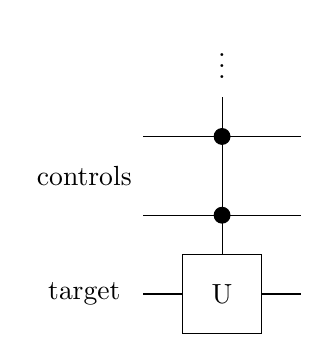
\begin{tikzpicture}[scale=.5] \node[draw=none] at (-3.5, 3) {controls}; \node[draw=none] at (-3.5, 0) {target}; \node[draw=none] at (0, 6) {$\vdots$}; \draw (0, 5) -- (0, 4); \draw (-2, 4) -- (2, 4); \draw[fill=black] (0, 4) circle (.2); \draw (0, 4) -- (0, 2); \draw (-2, 2) -- (2, 2); \draw[fill=black] (0, 2) circle (.2); \draw (0, 2) -- (0, 1); \draw (-2,0) -- (-1, 0); \draw (1, 0) -- (2, 0); \draw (-1,-1)--(-1,1)--(1,1)--(1,-1)--cycle; \node[draw=none] at (0, 0) {U}; \end{tikzpicture} } \]


\begin{DoxyParams}{Parameters}
\item[\mbox{$\leftrightarrow$} {\em multiQubit}]object representing the set of all qubits \item[\mbox{$\leftarrow$} {\em controlQubits}]applies unitary if all qubits in this array equal 1 \item[\mbox{$\leftarrow$} {\em numControlQubits}]number of control qubits \item[\mbox{$\leftarrow$} {\em targetQubit}]qubit to operate on \item[\mbox{$\leftarrow$} {\em u}]single-\/qubit unitary matrix to apply \end{DoxyParams}

\begin{DoxyExceptions}{Exceptions}
\item[{\em exitWithError}]if {\ttfamily numControlQubits} is outside \mbox{[}1, {\ttfamily multiQubit.numQubits}\mbox{]}), or if any qubit index ({\ttfamily targetQubit} or one in {\ttfamily controlQubits}) is outside \mbox{[}0, {\ttfamily multiQubit.numQubits}\mbox{]}), or if {\ttfamily controlQubits} contains {\ttfamily targetQubit}, or if {\ttfamily u} is not unitary. \end{DoxyExceptions}


Definition at line 143 of file qubits\_\-env\_\-local.c.

References MultiQubit::chunkId, chunkIsUpper(), exchangeStateVectors(), getChunkPairId(), getRotAngleFromUnitaryMatrix(), halfMatrixBlockFitsInChunk(), multiControlledUnitaryDistributed(), multiControlledUnitaryLocal(), MultiQubit::numAmps, MultiQubit::numQubits, MultiQubit::pairStateVec, QuESTAssert(), MultiQubit::stateVec, and validateMatrixIsUnitary().


\begin{DoxyCode}
144 {
145     QuESTAssert(targetQubit >= 0 && targetQubit < multiQubit.numQubits, 1, __func
      __);
146     QuESTAssert(numControlQubits > 0 && numControlQubits <= multiQubit.numQubits,
       4, __func__);
147     QuESTAssert(validateMatrixIsUnitary(u), 5, __func__);
148 
149     long long int mask=0; 
150     for (int i=0; i<numControlQubits; i++) mask = mask | (1LL<<controlQubits[i]);
      
151     QuESTAssert(mask >=0 && mask <= (1LL<<multiQubit.numQubits)-1, 2, __func__);
152     QuESTAssert((mask & (1LL<<targetQubit)) != (1LL<<targetQubit), 3, __func__);
153         
154     multiControlledUnitaryLocal(multiQubit, targetQubit, mask, u);
155 }
\end{DoxyCode}
\hypertarget{qubits_8h_aa5e77e0e64f3a4a3d3f5cc7382bffcd9}{
\index{qubits.h@{qubits.h}!reportMultiQubitParams@{reportMultiQubitParams}}
\index{reportMultiQubitParams@{reportMultiQubitParams}!qubits.h@{qubits.h}}
\paragraph[{reportMultiQubitParams}]{\setlength{\rightskip}{0pt plus 5cm}void reportMultiQubitParams ({\bf MultiQubit} {\em multiQubit})}\hfill}
\label{qubits_8h_aa5e77e0e64f3a4a3d3f5cc7382bffcd9}


Report metainformation about a set of qubits: number of qubits, number of probability amplitudes. 
\begin{DoxyParams}{Parameters}
\item[\mbox{$\leftrightarrow$} {\em multiQubit}]object representing the set of qubits \item[\mbox{$\leftarrow$} {\em env}]object representing the execution environment (local, multinode etc) \end{DoxyParams}


Definition at line 120 of file qubits.c.

References MultiQubit::chunkId, MultiQubit::numChunks, and MultiQubit::numQubits.


\begin{DoxyCode}
120                                                   {
121         long long int numAmps = 1L << multiQubit.numQubits;
122         long long int numAmpsPerRank = numAmps/multiQubit.numChunks;
123         if (multiQubit.chunkId==0){
124                 printf("QUBITS:\n");
125                 printf("Number of qubits is %d.\n", multiQubit.numQubits);
126                 printf("Number of amps is %lld.\n", numAmps);
127                 printf("Number of amps per rank is %lld.\n", numAmpsPerRank);
128         }
129 }
\end{DoxyCode}
\hypertarget{qubits_8h_af8a14ae79c3fb2c0b5f6255cc37bebf9}{
\index{qubits.h@{qubits.h}!reportQuESTEnv@{reportQuESTEnv}}
\index{reportQuESTEnv@{reportQuESTEnv}!qubits.h@{qubits.h}}
\paragraph[{reportQuESTEnv}]{\setlength{\rightskip}{0pt plus 5cm}void reportQuESTEnv ({\bf QuESTEnv} {\em env})}\hfill}
\label{qubits_8h_af8a14ae79c3fb2c0b5f6255cc37bebf9}


Report information about the QuEST environment. 
\begin{DoxyParams}{Parameters}
\item[\mbox{$\leftarrow$} {\em env}]object representing the execution environment. A single instance is used for each program \end{DoxyParams}


Definition at line 47 of file qubits\_\-env\_\-local.c.

References QuESTEnv::numRanks, QuESTEnv::rank, and REAL.


\begin{DoxyCode}
47                                  {
48         printf("EXECUTION ENVIRONMENT:\n");
49         printf("Running locally on one node\n");
50         printf("Number of ranks is %d\n", env.numRanks);
51 # ifdef _OPENMP
52         printf("OpenMP enabled\n");
53         printf("Number of threads available is %d\n", omp_get_max_threads());
54 # else
55         printf("OpenMP disabled\n");
56 # endif
57         printf("Precision: size of REAL is %ld bytes\n", sizeof(REAL));
58 }
\end{DoxyCode}
\hypertarget{qubits_8h_a96f4de9ce7fefc7680a44d601fc3d894}{
\index{qubits.h@{qubits.h}!reportState@{reportState}}
\index{reportState@{reportState}!qubits.h@{qubits.h}}
\paragraph[{reportState}]{\setlength{\rightskip}{0pt plus 5cm}void reportState ({\bf MultiQubit} {\em multiQubit})}\hfill}
\label{qubits_8h_a96f4de9ce7fefc7680a44d601fc3d894}


Print the current state vector of probability amplitudes for a set of qubits to file. File format: \begin{DoxyVerb}
real, imag
realComponent1, imagComponent1
realComponent2, imagComponent2
...
realComponentN, imagComponentN
\end{DoxyVerb}


File naming convention:

For each node that the program runs on, a file 'state\_\-rank\_\-\mbox{[}node\_\-rank\mbox{]}.csv' is generated. If there is more than one node, ranks after the first do not include the header \begin{DoxyVerb}
real, imag
\end{DoxyVerb}
 so that files are easier to combine.


\begin{DoxyParams}{Parameters}
\item[\mbox{$\leftrightarrow$} {\em multiQubit}]object representing the set of qubits \end{DoxyParams}


Definition at line 81 of file qubits.c.

References MultiQubit::chunkId, ComplexArray::imag, MultiQubit::numAmps, ComplexArray::real, REAL\_\-STRING\_\-FORMAT, and MultiQubit::stateVec.


\begin{DoxyCode}
81                                        {
82         FILE *state;
83         char filename[100];
84         long long int index;
85         sprintf(filename, "state_rank_%d.csv", multiQubit.chunkId);
86         state = fopen(filename, "w");
87         if (multiQubit.chunkId==0) fprintf(state, "real, imag\n");
88 
89         for(index=0; index<multiQubit.numAmps; index++){
90                 fprintf(state, REAL_STRING_FORMAT "," REAL_STRING_FORMAT "\n", mu
      ltiQubit.stateVec.real[index], multiQubit.stateVec.imag[index]);
91         }
92         fclose(state);
93 }
\end{DoxyCode}
\hypertarget{qubits_8h_a842d6884e063a5865a2232cba56b65ac}{
\index{qubits.h@{qubits.h}!reportStateToScreen@{reportStateToScreen}}
\index{reportStateToScreen@{reportStateToScreen}!qubits.h@{qubits.h}}
\paragraph[{reportStateToScreen}]{\setlength{\rightskip}{0pt plus 5cm}void reportStateToScreen ({\bf MultiQubit} {\em multiQubit}, \/  {\bf QuESTEnv} {\em env}, \/  int {\em reportRank})}\hfill}
\label{qubits_8h_a842d6884e063a5865a2232cba56b65ac}


Print the current state vector of probability amplitudes for a set of qubits to standard out. For debugging purposes. Each rank should print output serially. Only print output for systems $<$= 5 qubits 

Definition at line 95 of file qubits.c.

References MultiQubit::chunkId, ComplexArray::imag, MultiQubit::numAmps, MultiQubit::numChunks, MultiQubit::numQubits, ComplexArray::real, REAL\_\-STRING\_\-FORMAT, MultiQubit::stateVec, and syncQuESTEnv().


\begin{DoxyCode}
95                                                                              {
96         long long int index;
97         int rank;
98         if (multiQubit.numQubits<=5){
99                 for (rank=0; rank<multiQubit.numChunks; rank++){
100                         if (multiQubit.chunkId==rank){
101                                 if (reportRank) {
102                                         printf("Reporting state from rank %d [\n"
      , multiQubit.chunkId);
103                                         //printf("\trank, index, real, imag\n");
104                                         printf("real, imag\n");
105                                 } else if (rank==0) {
106                                         printf("Reporting state [\n");
107                                         printf("real, imag\n");
108                                 }
109 
110                                 for(index=0; index<multiQubit.numAmps; index++){
111                                         printf(REAL_STRING_FORMAT ", " 
      REAL_STRING_FORMAT "\n", multiQubit.stateVec.real[index], multiQubit.stateVec.
      imag[index]);
112                                 }
113                                 if (reportRank || rank==multiQubit.numChunks-1) p
      rintf("]\n");
114                         }
115                         syncQuESTEnv(env);
116                 }
117         } else printf("Error: reportStateToScreen will not print output for syste
      ms of more than 5 qubits.\n");
118 }
\end{DoxyCode}
\hypertarget{qubits_8h_a8810423457803005fecd415f4299f40d}{
\index{qubits.h@{qubits.h}!rotateAroundAxis@{rotateAroundAxis}}
\index{rotateAroundAxis@{rotateAroundAxis}!qubits.h@{qubits.h}}
\paragraph[{rotateAroundAxis}]{\setlength{\rightskip}{0pt plus 5cm}void rotateAroundAxis ({\bf MultiQubit} {\em multiQubit}, \/  const int {\em rotQubit}, \/  REAL {\em angle}, \/  {\bf Vector} {\em axis})}\hfill}
\label{qubits_8h_a8810423457803005fecd415f4299f40d}


Rotate a single qubit by a given angle around a given vector on the Bloch-\/sphere. The vector must not be zero (else an error is thrown), but needn't be unit magnitude.

For angle $\theta$ and axis vector $\vec{n}$, applies $R_{\hat{n}} = \exp \left(- i \frac{\theta}{2} \hat{n} \cdot \vec{\sigma} \right) $ where $\vec{\sigma}$ is the vector of Pauli matrices.


\begin{DoxyParams}{Parameters}
\item[\mbox{$\leftrightarrow$} {\em multiQubit}]object representing the set of all qubits \item[\mbox{$\leftarrow$} {\em rotQubit}]qubit to rotate \item[\mbox{$\leftarrow$} {\em angle}]angle by which to rotate in radians \item[\mbox{$\leftarrow$} {\em axis}]vector around which to rotate (can be non-\/unit; will be normalised) \end{DoxyParams}

\begin{DoxyExceptions}{Exceptions}
\item[{\em exitWithError}]if {\ttfamily rotQubit} is outside \mbox{[}0, {\ttfamily multiQubit.numQubits}), or if {\ttfamily axis} is the zero vector \end{DoxyExceptions}


Definition at line 382 of file qubits.c.

References compactUnitary(), Complex::imag, Complex::real, Vector::x, Vector::y, and Vector::z.

Referenced by rotateX(), rotateY(), and rotateZ().


\begin{DoxyCode}
382                                                                                  
              {
383         
384         double mag = sqrt(pow(axis.x,2) + pow(axis.y,2) + pow(axis.z,2));
385         Vector unitAxis = {axis.x/mag, axis.y/mag, axis.z/mag};
386         
387         Complex alpha, beta;
388         alpha.real = cos(angle/2.0);
389         alpha.imag = -sin(angle/2.0)*unitAxis.z;        
390         beta.real = sin(angle/2.0)*unitAxis.y;
391         beta.imag = -sin(angle/2.0)*unitAxis.x;
392         compactUnitary(multiQubit, rotQubit, alpha, beta);
393 }
\end{DoxyCode}
\hypertarget{qubits_8h_a6cc7fa705a2f2e6b486b49c5589d5df5}{
\index{qubits.h@{qubits.h}!rotateX@{rotateX}}
\index{rotateX@{rotateX}!qubits.h@{qubits.h}}
\paragraph[{rotateX}]{\setlength{\rightskip}{0pt plus 5cm}void rotateX ({\bf MultiQubit} {\em multiQubit}, \/  const int {\em rotQubit}, \/  REAL {\em angle})}\hfill}
\label{qubits_8h_a6cc7fa705a2f2e6b486b49c5589d5df5}


Rotate a single qubit by a given angle around the X-\/axis of the Bloch-\/sphere. For angle $\theta$, applies \[ \begin{pmatrix} \cos\theta/2 & -i \sin \theta/2\\ -i \sin \theta/2 & \cos \theta/2 \end{pmatrix} \]

\[ \setlength{\fboxrule}{0.01pt} \fbox{ 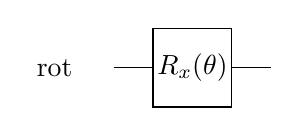
\begin{tikzpicture}[scale=.5] \node[draw=none] at (-3.5, 0) {rot}; \draw (-2,0) -- (-1, 0); \draw (1, 0) -- (2, 0); \draw (-1,-1)--(-1,1)--(1,1)--(1,-1)--cycle; \node[draw=none] at (0, 0) {$R_x(\theta)$}; \end{tikzpicture} } \]


\begin{DoxyParams}{Parameters}
\item[\mbox{$\leftrightarrow$} {\em multiQubit}]object representing the set of all qubits \item[\mbox{$\leftarrow$} {\em rotQubit}]qubit to rotate \item[\mbox{$\leftarrow$} {\em angle}]angle by which to rotate in radians \end{DoxyParams}

\begin{DoxyExceptions}{Exceptions}
\item[{\em exitWithError}]if {\ttfamily rotQubit} is outside \mbox{[}0, {\ttfamily multiQubit.numQubits}). \end{DoxyExceptions}


Definition at line 395 of file qubits.c.

References rotateAroundAxis().


\begin{DoxyCode}
395                                                                    {
396 
397         Vector unitAxis = {1, 0, 0};
398         rotateAroundAxis(multiQubit, rotQubit, angle, unitAxis);
399 }
\end{DoxyCode}
\hypertarget{qubits_8h_ace0d3592d38a990e81a434c4e9681500}{
\index{qubits.h@{qubits.h}!rotateY@{rotateY}}
\index{rotateY@{rotateY}!qubits.h@{qubits.h}}
\paragraph[{rotateY}]{\setlength{\rightskip}{0pt plus 5cm}void rotateY ({\bf MultiQubit} {\em multiQubit}, \/  const int {\em rotQubit}, \/  REAL {\em angle})}\hfill}
\label{qubits_8h_ace0d3592d38a990e81a434c4e9681500}


Rotate a single qubit by a given angle around the Y-\/axis of the Bloch-\/sphere. For angle $\theta$, applies \[ \begin{pmatrix} \cos\theta/2 & - \sin \theta/2\\ \sin \theta/2 & \cos \theta/2 \end{pmatrix} \]

\[ \setlength{\fboxrule}{0.01pt} \fbox{ 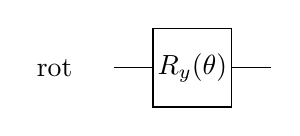
\begin{tikzpicture}[scale=.5] \node[draw=none] at (-3.5, 0) {rot}; \draw (-2,0) -- (-1, 0); \draw (1, 0) -- (2, 0); \draw (-1,-1)--(-1,1)--(1,1)--(1,-1)--cycle; \node[draw=none] at (0, 0) {$R_y(\theta)$}; \end{tikzpicture} } \]


\begin{DoxyParams}{Parameters}
\item[\mbox{$\leftrightarrow$} {\em multiQubit}]object representing the set of all qubits \item[\mbox{$\leftarrow$} {\em rotQubit}]qubit to rotate \item[\mbox{$\leftarrow$} {\em angle}]angle by which to rotate in radians \end{DoxyParams}

\begin{DoxyExceptions}{Exceptions}
\item[{\em exitWithError}]if {\ttfamily rotQubit} is outside \mbox{[}0, {\ttfamily multiQubit.numQubits}). \end{DoxyExceptions}


Definition at line 401 of file qubits.c.

References rotateAroundAxis().


\begin{DoxyCode}
401                                                                    {
402         
403         Vector unitAxis = {0, 1, 0};
404         rotateAroundAxis(multiQubit, rotQubit, angle, unitAxis);
405 }
\end{DoxyCode}
\hypertarget{qubits_8h_abd621412ad30c1b034f4ce153c4afe10}{
\index{qubits.h@{qubits.h}!rotateZ@{rotateZ}}
\index{rotateZ@{rotateZ}!qubits.h@{qubits.h}}
\paragraph[{rotateZ}]{\setlength{\rightskip}{0pt plus 5cm}void rotateZ ({\bf MultiQubit} {\em multiQubit}, \/  const int {\em rotQubit}, \/  REAL {\em angle})}\hfill}
\label{qubits_8h_abd621412ad30c1b034f4ce153c4afe10}


Rotate a single qubit by a given angle around the Z-\/axis of the Bloch-\/sphere (also known as a phase shift gate). For angle $\theta$, applies \[ \begin{pmatrix} \exp(-i \theta/2) & 0 \\ 0 & \exp(i \theta/2) \end{pmatrix} \]

\[ \setlength{\fboxrule}{0.01pt} \fbox{ 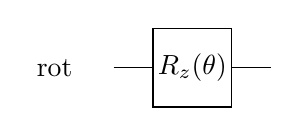
\begin{tikzpicture}[scale=.5] \node[draw=none] at (-3.5, 0) {rot}; \draw (-2,0) -- (-1, 0); \draw (1, 0) -- (2, 0); \draw (-1,-1)--(-1,1)--(1,1)--(1,-1)--cycle; \node[draw=none] at (0, 0) {$R_z(\theta)$}; \end{tikzpicture} } \]


\begin{DoxyParams}{Parameters}
\item[\mbox{$\leftrightarrow$} {\em multiQubit}]object representing the set of all qubits \item[\mbox{$\leftarrow$} {\em rotQubit}]qubit to rotate \item[\mbox{$\leftarrow$} {\em angle}]angle by which to rotate in radians \end{DoxyParams}

\begin{DoxyExceptions}{Exceptions}
\item[{\em exitWithError}]if {\ttfamily rotQubit} is outside \mbox{[}0, {\ttfamily multiQubit.numQubits}). \end{DoxyExceptions}


Definition at line 407 of file qubits.c.

References rotateAroundAxis().


\begin{DoxyCode}
407                                                                    {
408         
409         Vector unitAxis = {0, 0, 1};
410         rotateAroundAxis(multiQubit, rotQubit, angle, unitAxis);
411 }
\end{DoxyCode}
\hypertarget{qubits_8h_adda6c47876a7676488ed0565a19eaa65}{
\index{qubits.h@{qubits.h}!sGate@{sGate}}
\index{sGate@{sGate}!qubits.h@{qubits.h}}
\paragraph[{sGate}]{\setlength{\rightskip}{0pt plus 5cm}void sGate ({\bf MultiQubit} {\em multiQubit}, \/  const int {\em targetQubit})}\hfill}
\label{qubits_8h_adda6c47876a7676488ed0565a19eaa65}


Apply the single-\/qubit S gate. This is a rotation of $\pi/2$ around the Z-\/axis on the Bloch sphere, or the unitary: \[ \begin{pmatrix} 1 & 0 \\ 0 & i \end{pmatrix} \]

\[ \setlength{\fboxrule}{0.01pt} \fbox{ 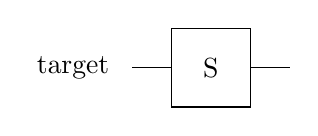
\begin{tikzpicture}[scale=.5] \node[draw=none] at (-3.5, 0) {target}; \draw (-2,0) -- (-1, 0); \draw (1, 0) -- (2, 0); \draw (-1,-1)--(-1,1)--(1,1)--(1,-1)--cycle; \node[draw=none] at (0, 0) {S}; \end{tikzpicture} } \]


\begin{DoxyParams}{Parameters}
\item[\mbox{$\leftrightarrow$} {\em multiQubit}]object representing the set of all qubits \item[\mbox{$\leftarrow$} {\em targetQubit}]qubit to operate upon \end{DoxyParams}

\begin{DoxyExceptions}{Exceptions}
\item[{\em exitWithError}]if {\ttfamily targetQubit} is outside \mbox{[}0, {\ttfamily multiQubit.numQubits}) \end{DoxyExceptions}


Definition at line 1580 of file qubits.c.

References phaseGate(), and S\_\-GATE.


\begin{DoxyCode}
1581 {
1582                 phaseGate(multiQubit, targetQubit, S_GATE);
1583 } 
\end{DoxyCode}
\hypertarget{qubits_8h_a86e396e06b7d527cac20ba0108872423}{
\index{qubits.h@{qubits.h}!sigmaX@{sigmaX}}
\index{sigmaX@{sigmaX}!qubits.h@{qubits.h}}
\paragraph[{sigmaX}]{\setlength{\rightskip}{0pt plus 5cm}void sigmaX ({\bf MultiQubit} {\em multiQubit}, \/  const int {\em targetQubit})}\hfill}
\label{qubits_8h_a86e396e06b7d527cac20ba0108872423}


Apply the single-\/qubit sigma-\/X (also known as the X, Pauli-\/X, NOT or bit-\/flip) gate. This is a rotation of $\pi$ around the x-\/axis on the Bloch sphere. I.e. \[ \begin{pmatrix} 0 & 1 \\ 1 & 0 \end{pmatrix} \]

\[ \setlength{\fboxrule}{0.01pt} \fbox{ 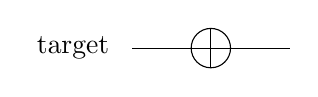
\begin{tikzpicture}[scale=.5] \node[draw=none] at (-3.5, 0) {target}; \draw (-2,0) -- (2, 0); \draw (0, 0) circle (.5); \draw (0, .5) -- (0, -.5); \end{tikzpicture} } \]


\begin{DoxyParams}{Parameters}
\item[\mbox{$\leftrightarrow$} {\em multiQubit}]object representing the set of all qubits \item[\mbox{$\leftarrow$} {\em targetQubit}]qubit to operate on \end{DoxyParams}

\begin{DoxyExceptions}{Exceptions}
\item[{\em exitWithError}]if {\ttfamily targetQubit} is outside \mbox{[}0, {\ttfamily multiQubit.numQubits}). \end{DoxyExceptions}


Definition at line 157 of file qubits\_\-env\_\-local.c.

References MultiQubit::chunkId, chunkIsUpper(), exchangeStateVectors(), getChunkPairId(), halfMatrixBlockFitsInChunk(), MultiQubit::numAmps, MultiQubit::numQubits, MultiQubit::pairStateVec, QuESTAssert(), sigmaXDistributed(), sigmaXLocal(), and MultiQubit::stateVec.


\begin{DoxyCode}
158 {
159     QuESTAssert(targetQubit >= 0 && targetQubit < multiQubit.numQubits, 1, __func
      __);
160         sigmaXLocal(multiQubit, targetQubit);
161 }
\end{DoxyCode}
\hypertarget{qubits_8h_a1f54d70a42403f7e1c2e2c2007332f61}{
\index{qubits.h@{qubits.h}!sigmaY@{sigmaY}}
\index{sigmaY@{sigmaY}!qubits.h@{qubits.h}}
\paragraph[{sigmaY}]{\setlength{\rightskip}{0pt plus 5cm}void sigmaY ({\bf MultiQubit} {\em multiQubit}, \/  const int {\em targetQubit})}\hfill}
\label{qubits_8h_a1f54d70a42403f7e1c2e2c2007332f61}


Apply the single-\/qubit sigma-\/Y (also known as the Y or Pauli-\/Y) gate. This is a rotation of $\pi$ around the Y-\/axis on the Bloch sphere. I.e. \[ \begin{pmatrix} 0 & -i \\ i & 0 \end{pmatrix} \]

\[ \setlength{\fboxrule}{0.01pt} \fbox{ 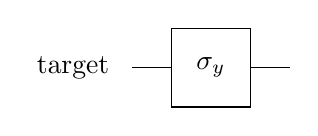
\begin{tikzpicture}[scale=.5] \node[draw=none] at (-3.5, 0) {target}; \draw (-2,0) -- (-1, 0); \draw (1, 0) -- (2, 0); \draw (-1,-1)--(-1,1)--(1,1)--(1,-1)--cycle; \node[draw=none] at (0, 0) {$\sigma_y$}; \end{tikzpicture} } \]


\begin{DoxyParams}{Parameters}
\item[\mbox{$\leftrightarrow$} {\em multiQubit}]object representing the set of all qubits \item[\mbox{$\leftarrow$} {\em targetQubit}]qubit to operate on \end{DoxyParams}

\begin{DoxyExceptions}{Exceptions}
\item[{\em exitWithError}]if {\ttfamily targetQubit} is outside \mbox{[}0, {\ttfamily multiQubit.numQubits}). \end{DoxyExceptions}


fix -\/-\/ put duplicate code (sigmaX, sigmaY) in seperate function 

Definition at line 163 of file qubits\_\-env\_\-local.c.

References MultiQubit::chunkId, chunkIsUpper(), exchangeStateVectors(), getChunkPairId(), halfMatrixBlockFitsInChunk(), MultiQubit::numAmps, MultiQubit::numQubits, MultiQubit::pairStateVec, QuESTAssert(), sigmaYDistributed(), sigmaYLocal(), and MultiQubit::stateVec.


\begin{DoxyCode}
164 {
165     QuESTAssert(targetQubit >= 0 && targetQubit < multiQubit.numQubits, 1, __func
      __);
166         sigmaYLocal(multiQubit, targetQubit);
167 }
\end{DoxyCode}
\hypertarget{qubits_8h_aebaab86326779de55d335cfea3efde8f}{
\index{qubits.h@{qubits.h}!sigmaZ@{sigmaZ}}
\index{sigmaZ@{sigmaZ}!qubits.h@{qubits.h}}
\paragraph[{sigmaZ}]{\setlength{\rightskip}{0pt plus 5cm}void sigmaZ ({\bf MultiQubit} {\em multiQubit}, \/  const int {\em targetQubit})}\hfill}
\label{qubits_8h_aebaab86326779de55d335cfea3efde8f}


Apply the single-\/qubit sigma-\/Z (also known as the Z, Pauli-\/Z or phase-\/flip) gate. This is a rotation of $\pi$ around the Z-\/axis (a phase shift) on the Bloch sphere. I.e. \[ \begin{pmatrix} 1 & 0 \\ 0 & -1 \end{pmatrix} \]

\[ \setlength{\fboxrule}{0.01pt} \fbox{ 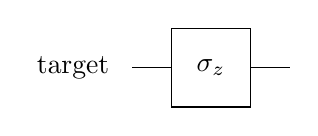
\begin{tikzpicture}[scale=.5] \node[draw=none] at (-3.5, 0) {target}; \draw (-2,0) -- (-1, 0); \draw (1, 0) -- (2, 0); \draw (-1,-1)--(-1,1)--(1,1)--(1,-1)--cycle; \node[draw=none] at (0, 0) {$\sigma_z$}; \end{tikzpicture} } \]


\begin{DoxyParams}{Parameters}
\item[\mbox{$\leftrightarrow$} {\em multiQubit}]object representing the set of all qubits \item[\mbox{$\leftarrow$} {\em targetQubit}]qubit to operate on \end{DoxyParams}

\begin{DoxyExceptions}{Exceptions}
\item[{\em exitWithError}]if {\ttfamily targetQubit} is outside \mbox{[}0, {\ttfamily multiQubit.numQubits}). \end{DoxyExceptions}


Definition at line 1575 of file qubits.c.

References phaseGate(), and SIGMA\_\-Z.


\begin{DoxyCode}
1576 {
1577                 phaseGate(multiQubit, targetQubit, SIGMA_Z);
1578 }
\end{DoxyCode}
\hypertarget{qubits_8h_a8d31fe2d1ad4d01e2a1f5f6b8bc15b77}{
\index{qubits.h@{qubits.h}!syncQuESTEnv@{syncQuESTEnv}}
\index{syncQuESTEnv@{syncQuESTEnv}!qubits.h@{qubits.h}}
\paragraph[{syncQuESTEnv}]{\setlength{\rightskip}{0pt plus 5cm}void syncQuESTEnv ({\bf QuESTEnv} {\em env})}\hfill}
\label{qubits_8h_a8d31fe2d1ad4d01e2a1f5f6b8bc15b77}


Guarantees that all code up to the given point has been executed on all nodes (if running in distributed mode). 
\begin{DoxyParams}{Parameters}
\item[\mbox{$\leftarrow$} {\em env}]object representing the execution environment. A single instance is used for each program \end{DoxyParams}


Definition at line 35 of file qubits\_\-env\_\-local.c.

Referenced by initializeStateFromSingleFile(), and reportStateToScreen().


\begin{DoxyCode}
35                                {
36         // MPI Barrier goes here in MPI version. 
37 } 
\end{DoxyCode}
\hypertarget{qubits_8h_ac7e38d768a1bd79019f88cc1e6295092}{
\index{qubits.h@{qubits.h}!syncQuESTSuccess@{syncQuESTSuccess}}
\index{syncQuESTSuccess@{syncQuESTSuccess}!qubits.h@{qubits.h}}
\paragraph[{syncQuESTSuccess}]{\setlength{\rightskip}{0pt plus 5cm}int syncQuESTSuccess (int {\em successCode})}\hfill}
\label{qubits_8h_ac7e38d768a1bd79019f88cc1e6295092}


Performs a logical AND on all successCodes held by all processes. If any one process has a zero successCode all processes will return a zero success code.


\begin{DoxyParams}{Parameters}
\item[\mbox{$\leftarrow$} {\em env}]object representing the execution environment. A single instance is used for each program \item[\mbox{$\leftarrow$} {\em successCode}]1 if process task succeeded, 0 if process task failed \end{DoxyParams}
\begin{DoxyReturn}{Returns}
1 if all processes succeeded, 0 if any one process failed 
\end{DoxyReturn}


Definition at line 39 of file qubits\_\-env\_\-local.c.


\begin{DoxyCode}
39                                      {
40         return successCode;
41 }
\end{DoxyCode}
\hypertarget{qubits_8h_af764ea63a2e870098f4e1ce08562942e}{
\index{qubits.h@{qubits.h}!tGate@{tGate}}
\index{tGate@{tGate}!qubits.h@{qubits.h}}
\paragraph[{tGate}]{\setlength{\rightskip}{0pt plus 5cm}void tGate ({\bf MultiQubit} {\em multiQubit}, \/  const int {\em targetQubit})}\hfill}
\label{qubits_8h_af764ea63a2e870098f4e1ce08562942e}


Apply the single-\/qubit T gate. This is a rotation of $\pi/4$ around the Z-\/axis on the Bloch sphere, or the unitary: \[ \begin{pmatrix} 1 & 0 \\ 0 & \exp\left(i \frac{\pi}{4}\right) \end{pmatrix} \]

\[ \setlength{\fboxrule}{0.01pt} \fbox{ 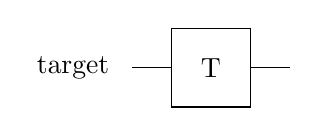
\begin{tikzpicture}[scale=.5] \node[draw=none] at (-3.5, 0) {target}; \draw (-2,0) -- (-1, 0); \draw (1, 0) -- (2, 0); \draw (-1,-1)--(-1,1)--(1,1)--(1,-1)--cycle; \node[draw=none] at (0, 0) {T}; \end{tikzpicture} } \]


\begin{DoxyParams}{Parameters}
\item[\mbox{$\leftrightarrow$} {\em multiQubit}]object representing the set of all qubits \item[\mbox{$\leftarrow$} {\em targetQubit}]qubit to operate upon \end{DoxyParams}

\begin{DoxyExceptions}{Exceptions}
\item[{\em exitWithError}]if {\ttfamily targetQubit} is outside \mbox{[}0, {\ttfamily multiQubit.numQubits}) \end{DoxyExceptions}


Definition at line 1585 of file qubits.c.

References phaseGate(), and T\_\-GATE.


\begin{DoxyCode}
1586 {
1587                 phaseGate(multiQubit, targetQubit, T_GATE);
1588 }
\end{DoxyCode}
\hypertarget{qubits_8h_a7a0877e33700f6bad48adb51b7b3fb67}{
\index{qubits.h@{qubits.h}!unitary@{unitary}}
\index{unitary@{unitary}!qubits.h@{qubits.h}}
\paragraph[{unitary}]{\setlength{\rightskip}{0pt plus 5cm}void unitary ({\bf MultiQubit} {\em multiQubit}, \/  const int {\em targetQubit}, \/  {\bf ComplexMatrix2} {\em u})}\hfill}
\label{qubits_8h_a7a0877e33700f6bad48adb51b7b3fb67}


Apply a general single-\/qubit unitary (including a global phase factor). The passed 2x2 ComplexMatrix must be unitary, otherwise an error is thrown.

\[ \setlength{\fboxrule}{0.01pt} \fbox{ 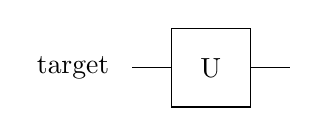
\begin{tikzpicture}[scale=.5] \node[draw=none] at (-3.5, 0) {target}; \draw (-2,0) -- (-1, 0); \draw (1, 0) -- (2, 0); \draw (-1,-1)--(-1,1)--(1,1)--(1,-1)--cycle; \node[draw=none] at (0, 0) {U}; \end{tikzpicture} } \]


\begin{DoxyParams}{Parameters}
\item[\mbox{$\leftrightarrow$} {\em multiQubit}]object representing the set of all qubits \item[\mbox{$\leftarrow$} {\em targetQubit}]qubit to operate on \item[\mbox{$\leftarrow$} {\em u}]unitary matrix to apply \end{DoxyParams}

\begin{DoxyExceptions}{Exceptions}
\item[{\em exitWithError}]if {\ttfamily targetQubit} is outside \mbox{[}0, {\ttfamily multiQubit.numQubits}), or matrix {\ttfamily u} is not unitary. \end{DoxyExceptions}


Definition at line 113 of file qubits\_\-env\_\-local.c.

References MultiQubit::chunkId, chunkIsUpper(), exchangeStateVectors(), getChunkPairId(), getRotAngleFromUnitaryMatrix(), halfMatrixBlockFitsInChunk(), MultiQubit::numAmps, MultiQubit::numQubits, MultiQubit::pairStateVec, QuESTAssert(), MultiQubit::stateVec, unitaryDistributed(), unitaryLocal(), and validateMatrixIsUnitary().


\begin{DoxyCode}
114 {
115     QuESTAssert(targetQubit >= 0 && targetQubit < multiQubit.numQubits, 1, __func
      __);
116     QuESTAssert(validateMatrixIsUnitary(u), 5, __func__);
117 
118         // all values required to update state vector lie in this rank
119         unitaryLocal(multiQubit, targetQubit, u);
120 }
\end{DoxyCode}

\hypertarget{qubits__debug_8h}{
\subsection{qubits\_\-debug.h File Reference}
\label{qubits__debug_8h}\index{qubits\_\-debug.h@{qubits\_\-debug.h}}
}


Developer functions used for unit testing and debugging.  
{\ttfamily \#include \char`\"{}precision.h\char`\"{}}\par
\subsubsection*{Functions}
\begin{DoxyCompactItemize}
\item 
void \hyperlink{qubits__debug_8h_a7169fd0442cbc3418f3fac4d13363ca2}{initStateOfSingleQubit} (\hyperlink{structMultiQubit}{MultiQubit} $\ast$multiQubit, int qubitId, int outcome)
\begin{DoxyCompactList}\small\item\em Initialise the state vector of probability amplitudes such that one qubit is set to 'outcome' and all other qubits are in an equal superposition of zero and one. \item\end{DoxyCompactList}\item 
void \hyperlink{qubits__debug_8h_a03b3577a891731d505bc4b879fcca9d3}{initStateDebug} (\hyperlink{structMultiQubit}{MultiQubit} $\ast$multiQubit)
\begin{DoxyCompactList}\small\item\em Initialise the state vector of probability amplitudes to an (unphysical) state with each component of each probability amplitude a unique floating point value. \item\end{DoxyCompactList}\item 
void \hyperlink{qubits__debug_8h_a433876ee9f3bcc54af346300f571fc3c}{initializeStateFromSingleFile} (\hyperlink{structMultiQubit}{MultiQubit} $\ast$multiQubit, char filename\mbox{[}200\mbox{]}, \hyperlink{structQuESTEnv}{QuESTEnv} env)
\item 
int \hyperlink{qubits__debug_8h_a793584932ae384c82e7e42db7d35d18d}{compareStates} (\hyperlink{structMultiQubit}{MultiQubit} mq1, \hyperlink{structMultiQubit}{MultiQubit} mq2, REAL precision)
\item 
void \hyperlink{qubits__debug_8h_a62da5b58d8ce84e6f4d24be1b872294e}{reportNodeList} (\hyperlink{structQuESTEnv}{QuESTEnv} env)
\begin{DoxyCompactList}\small\item\em Report a list of CPU hostnames and the rank that is running on each if running with MPI enabled and an error message otherwise. \item\end{DoxyCompactList}\end{DoxyCompactItemize}


\subsubsection{Detailed Description}
Developer functions used for unit testing and debugging. Not part of the public API. May contain functions that are incomplete or untested. 

Definition in file \hyperlink{qubits__debug_8h_source}{qubits\_\-debug.h}.

\subsubsection{Function Documentation}
\hypertarget{qubits__debug_8h_a793584932ae384c82e7e42db7d35d18d}{
\index{qubits\_\-debug.h@{qubits\_\-debug.h}!compareStates@{compareStates}}
\index{compareStates@{compareStates}!qubits_debug.h@{qubits\_\-debug.h}}
\paragraph[{compareStates}]{\setlength{\rightskip}{0pt plus 5cm}int compareStates ({\bf MultiQubit} {\em mq1}, \/  {\bf MultiQubit} {\em mq2}, \/  REAL {\em precision})}\hfill}
\label{qubits__debug_8h_a793584932ae384c82e7e42db7d35d18d}


Definition at line 327 of file qubits.c.

References ComplexArray::imag, MultiQubit::numAmps, ComplexArray::real, REAL, and MultiQubit::stateVec.


\begin{DoxyCode}
327                                                                  {
328         REAL diff;
329         int chunkSize = mq1.numAmps;
330         for (int i=0; i<chunkSize; i++){
331                 diff = mq1.stateVec.real[i] - mq2.stateVec.real[i];
332                 if (diff<0) diff *= -1;
333                 if (diff>precision) return 0;
334                 diff = mq1.stateVec.imag[i] - mq2.stateVec.imag[i];
335                 if (diff<0) diff *= -1;
336                 if (diff>precision) return 0;
337         }
338         return 1;
339 }
\end{DoxyCode}
\hypertarget{qubits__debug_8h_a433876ee9f3bcc54af346300f571fc3c}{
\index{qubits\_\-debug.h@{qubits\_\-debug.h}!initializeStateFromSingleFile@{initializeStateFromSingleFile}}
\index{initializeStateFromSingleFile@{initializeStateFromSingleFile}!qubits_debug.h@{qubits\_\-debug.h}}
\paragraph[{initializeStateFromSingleFile}]{\setlength{\rightskip}{0pt plus 5cm}void initializeStateFromSingleFile ({\bf MultiQubit} $\ast$ {\em multiQubit}, \/  char {\em filename}\mbox{[}200\mbox{]}, \/  {\bf QuESTEnv} {\em env})}\hfill}
\label{qubits__debug_8h_a433876ee9f3bcc54af346300f571fc3c}


fix -\/-\/ format needs to work for single precision values 

Definition at line 292 of file qubits.c.

References MultiQubit::chunkId, ComplexArray::imag, MultiQubit::numAmps, MultiQubit::numChunks, ComplexArray::real, REAL, MultiQubit::stateVec, and syncQuESTEnv().


\begin{DoxyCode}
292                                                                                  
                 {
293         long long int chunkSize, stateVecSize;
294         long long int indexInChunk, totalIndex;
295 
296         chunkSize = multiQubit->numAmps;
297         stateVecSize = chunkSize*multiQubit->numChunks;
298 
299         REAL *stateVecReal = multiQubit->stateVec.real;
300         REAL *stateVecImag = multiQubit->stateVec.imag;
301         
302         FILE *fp;
303         char line[200];
304 
305         for (int rank=0; rank<(multiQubit->numChunks); rank++){
306                 if (rank==multiQubit->chunkId){
307                         fp = fopen(filename, "r");
308                         indexInChunk = 0; totalIndex = 0;
309                         while (fgets(line, sizeof(char)*200, fp) != NULL && total
      Index<stateVecSize){
310                                 if (line[0]!='#'){
311                                         int chunkId = totalIndex/chunkSize;
312                                         if (chunkId==multiQubit->chunkId){
314                                                 sscanf(line, "%lf, %lf", &(stateV
      ecReal[indexInChunk]), 
315                                                                 &(stateVecImag[in
      dexInChunk]));
316                                                 indexInChunk += 1;
317                                         }
318                                         totalIndex += 1;
319                                 }
320                         }       
321                         fclose(fp);
322                 }
323                 syncQuESTEnv(env);
324         }
325 }
\end{DoxyCode}
\hypertarget{qubits__debug_8h_a03b3577a891731d505bc4b879fcca9d3}{
\index{qubits\_\-debug.h@{qubits\_\-debug.h}!initStateDebug@{initStateDebug}}
\index{initStateDebug@{initStateDebug}!qubits_debug.h@{qubits\_\-debug.h}}
\paragraph[{initStateDebug}]{\setlength{\rightskip}{0pt plus 5cm}void initStateDebug ({\bf MultiQubit} $\ast$ {\em multiQubit})}\hfill}
\label{qubits__debug_8h_a03b3577a891731d505bc4b879fcca9d3}


Initialise the state vector of probability amplitudes to an (unphysical) state with each component of each probability amplitude a unique floating point value. For debugging processes 
\begin{DoxyParams}{Parameters}
\item[\mbox{$\leftrightarrow$} {\em multiQubit}]object representing the set of qubits to be initialised \end{DoxyParams}


Definition at line 260 of file qubits.c.

References MultiQubit::chunkId, ComplexArray::imag, MultiQubit::numAmps, ComplexArray::real, REAL, and MultiQubit::stateVec.


\begin{DoxyCode}
261 {
262         long long int chunkSize;
263         long long int index;
264 
265         // dimension of the state vector
266         chunkSize = multiQubit->numAmps;
267 
268         // Can't use multiQubit->stateVec as a private OMP var
269         REAL *stateVecReal = multiQubit->stateVec.real;
270         REAL *stateVecImag = multiQubit->stateVec.imag;
271 
272         REAL chunkOffset = (2.0*chunkSize*multiQubit->chunkId)/10.0;
273 
274         // initialise the state to |0000..0000>
275 # ifdef _OPENMP
276 # pragma omp parallel \
277         default  (none) \
278         shared   (chunkSize, stateVecReal, stateVecImag, chunkOffset) \
279         private  (index) 
280 # endif
281         {
282 # ifdef _OPENMP
283                 # pragma omp for schedule (static)
284 # endif
285                 for (index=0; index<chunkSize; index++) {
286                         stateVecReal[index] = chunkOffset + (index*2.0)/10.0;
287                         stateVecImag[index] = chunkOffset + (index*2.0+1.0)/10.0;
      
288                 }
289         }
290 }
\end{DoxyCode}
\hypertarget{qubits__debug_8h_a7169fd0442cbc3418f3fac4d13363ca2}{
\index{qubits\_\-debug.h@{qubits\_\-debug.h}!initStateOfSingleQubit@{initStateOfSingleQubit}}
\index{initStateOfSingleQubit@{initStateOfSingleQubit}!qubits_debug.h@{qubits\_\-debug.h}}
\paragraph[{initStateOfSingleQubit}]{\setlength{\rightskip}{0pt plus 5cm}void initStateOfSingleQubit ({\bf MultiQubit} $\ast$ {\em multiQubit}, \/  int {\em qubitId}, \/  int {\em outcome})}\hfill}
\label{qubits__debug_8h_a7169fd0442cbc3418f3fac4d13363ca2}


Initialise the state vector of probability amplitudes such that one qubit is set to 'outcome' and all other qubits are in an equal superposition of zero and one. 
\begin{DoxyParams}{Parameters}
\item[\mbox{$\leftrightarrow$} {\em multiQubit}]object representing the set of qubits to be initialised \item[\mbox{$\leftarrow$} {\em qubitId}]id of qubit to set to state 'outcome' \item[\mbox{$\leftarrow$} {\em value}]of qubit 'qubitId' \end{DoxyParams}


Definition at line 213 of file qubits.c.

References MultiQubit::chunkId, DEBUG, extractBit(), ComplexArray::imag, MultiQubit::numAmps, MultiQubit::numChunks, ComplexArray::real, REAL, and MultiQubit::stateVec.


\begin{DoxyCode}
214 {
215         long long int chunkSize, stateVecSize;
216         long long int index;
217         int bit;
218         const long long int chunkId=multiQubit->chunkId;
219 
220         // dimension of the state vector
221         chunkSize = multiQubit->numAmps;
222         stateVecSize = chunkSize*multiQubit->numChunks;
223         REAL normFactor = 1.0/sqrt((REAL)stateVecSize/2.0);
224 
225         // Can't use multiQubit->stateVec as a private OMP var
226         REAL *stateVecReal = multiQubit->stateVec.real;
227         REAL *stateVecImag = multiQubit->stateVec.imag;
228 
229         // initialise the state to |0000..0000>
230 # ifdef _OPENMP
231 # pragma omp parallel \
232         default  (none) \
233         shared   (chunkSize, stateVecReal, stateVecImag, normFactor, qubitId, out
      come) \
234         private  (index, bit) 
235 # endif
236         {
237 # ifdef _OPENMP
238                 # pragma omp for schedule (static)
239 # endif
240                 for (index=0; index<chunkSize; index++) {
241                         bit = extractBit(qubitId, index+chunkId*chunkSize);
242                         if (bit==outcome) {
243                                 stateVecReal[index] = normFactor;
244                                 stateVecImag[index] = 0.0;
245                         } else {
246                                 stateVecReal[index] = 0.0;
247                                 stateVecImag[index] = 0.0;
248                         }
249                 }
250         }
251         if (DEBUG) printf("COMPLETED INIT\n");
252 }
\end{DoxyCode}
\hypertarget{qubits__debug_8h_a62da5b58d8ce84e6f4d24be1b872294e}{
\index{qubits\_\-debug.h@{qubits\_\-debug.h}!reportNodeList@{reportNodeList}}
\index{reportNodeList@{reportNodeList}!qubits_debug.h@{qubits\_\-debug.h}}
\paragraph[{reportNodeList}]{\setlength{\rightskip}{0pt plus 5cm}void reportNodeList ({\bf QuESTEnv} {\em env})}\hfill}
\label{qubits__debug_8h_a62da5b58d8ce84e6f4d24be1b872294e}


Report a list of CPU hostnames and the rank that is running on each if running with MPI enabled and an error message otherwise. For debugging purposes. 
\begin{DoxyParams}{Parameters}
\item[\mbox{$\leftarrow$} {\em env}]object representing the execution environment. A single instance is used for each program \end{DoxyParams}


Definition at line 57 of file qubits\_\-env\_\-local.c.

References QuESTEnv::rank.


\begin{DoxyCode}
57                                  {
58         printf("Hostname unknown: running locally\n");
59 }
\end{DoxyCode}

\hypertarget{qubits__env__local_8c}{}\subsection{qubits\+\_\+env\+\_\+local.\+c File Reference}
\label{qubits__env__local_8c}\index{qubits\+\_\+env\+\_\+local.\+c@{qubits\+\_\+env\+\_\+local.\+c}}


An implementation of the A\+PI in \hyperlink{qubits_8h}{qubits.\+h} for a local (non-\/\+M\+PI) environment.  


{\ttfamily \#include $<$stdlib.\+h$>$}\\*
{\ttfamily \#include \char`\"{}qubits.\+h\char`\"{}}\\*
{\ttfamily \#include \char`\"{}qubits\+\_\+internal.\+h\char`\"{}}\\*
\subsubsection*{Functions}
\begin{DoxyCompactItemize}
\item 
void \hyperlink{qubits__env__local_8c_a652d8c53f8f1cfb096133791de2b219d}{init\+Q\+U\+E\+S\+T\+Env} (\hyperlink{structQUESTEnv}{Q\+U\+E\+S\+T\+Env} $\ast$env)
\begin{DoxyCompactList}\small\item\em Initialize Q\+U\+E\+ST environment. \end{DoxyCompactList}\item 
void \hyperlink{qubits__env__local_8c_a83dffc500bf5b4e41dd63ba1ea9422ae}{sync\+Q\+U\+E\+S\+T\+Env} (\hyperlink{structQUESTEnv}{Q\+U\+E\+S\+T\+Env} env)
\begin{DoxyCompactList}\small\item\em Guarantees that all code up to the given point has been executed on all nodes. \end{DoxyCompactList}\item 
void \hyperlink{qubits__env__local_8c_ad7494473d827399d7fd9c327ea3a23e6}{close\+Q\+U\+E\+S\+T\+Env} (\hyperlink{structQUESTEnv}{Q\+U\+E\+S\+T\+Env} env)
\begin{DoxyCompactList}\small\item\em Close Q\+U\+E\+ST environment. \end{DoxyCompactList}\item 
void \hyperlink{qubits__env__local_8c_aa5d0566a6ef6519ff7b5241915fbf170}{report\+Q\+U\+E\+S\+T\+Env} (\hyperlink{structQUESTEnv}{Q\+U\+E\+S\+T\+Env} env)
\begin{DoxyCompactList}\small\item\em Report information about the Q\+U\+E\+ST environment. \end{DoxyCompactList}\item 
double \hyperlink{qubits__env__local_8c_a2205c8fde15213df52040dc3df233090}{calc\+Total\+Probability} (\hyperlink{structMultiQubit}{Multi\+Qubit} multi\+Qubit)
\begin{DoxyCompactList}\small\item\em Calculate the probability of being in any state by taking the norm of the entire state vector. \end{DoxyCompactList}\item 
void \hyperlink{qubits__env__local_8c_a4ba468aa69f812efd1f964e10a45ca2f}{rotate\+Qubit} (\hyperlink{structMultiQubit}{Multi\+Qubit} multi\+Qubit, const int rot\+Qubit, \hyperlink{structComplex}{Complex} alpha, \hyperlink{structComplex}{Complex} beta)
\begin{DoxyCompactList}\small\item\em Rotate a single qubit in the state vector of probability amplitudes, given the angle rotation arguments. \end{DoxyCompactList}\item 
double \hyperlink{qubits__env__local_8c_af31016680d01044cee9321d4cae32703}{find\+Probability\+Of\+Zero} (\hyperlink{structMultiQubit}{Multi\+Qubit} multi\+Qubit, const int measure\+Qubit)
\begin{DoxyCompactList}\small\item\em Measure the probability of a specified qubit being in the zero state. \end{DoxyCompactList}\end{DoxyCompactItemize}


\subsubsection{Detailed Description}
An implementation of the A\+PI in \hyperlink{qubits_8h}{qubits.\+h} for a local (non-\/\+M\+PI) environment. 



\subsubsection{Function Documentation}
\index{qubits\+\_\+env\+\_\+local.\+c@{qubits\+\_\+env\+\_\+local.\+c}!calc\+Total\+Probability@{calc\+Total\+Probability}}
\index{calc\+Total\+Probability@{calc\+Total\+Probability}!qubits\+\_\+env\+\_\+local.\+c@{qubits\+\_\+env\+\_\+local.\+c}}
\paragraph[{\texorpdfstring{calc\+Total\+Probability(\+Multi\+Qubit multi\+Qubit)}{calcTotalProbability(MultiQubit multiQubit)}}]{\setlength{\rightskip}{0pt plus 5cm}double calc\+Total\+Probability (
\begin{DoxyParamCaption}
\item[{{\bf Multi\+Qubit}}]{multi\+Qubit}
\end{DoxyParamCaption}
)}\hypertarget{qubits__env__local_8c_a2205c8fde15213df52040dc3df233090}{}\label{qubits__env__local_8c_a2205c8fde15213df52040dc3df233090}


Calculate the probability of being in any state by taking the norm of the entire state vector. 

Should be equal to 1. 
\begin{DoxyParams}[1]{Parameters}
\mbox{\tt in}  & {\em multi\+Qubit} & object representing a set of qubits \\
\hline
\end{DoxyParams}
\begin{DoxyReturn}{Returns}
total probability 
\end{DoxyReturn}


Definition at line 36 of file qubits\+\_\+env\+\_\+local.\+c.



References Complex\+Array\+::imag, Multi\+Qubit\+::num\+Amps, Complex\+Array\+::real, and Multi\+Qubit\+::state\+Vec.


\begin{DoxyCode}
36                                                   \{
37         \textcolor{keywordtype}{double} pTotal=0; 
38         \textcolor{keywordtype}{long} \textcolor{keywordtype}{long} \textcolor{keywordtype}{int} index;
39         \textcolor{keywordtype}{long} \textcolor{keywordtype}{long} \textcolor{keywordtype}{int} numAmpsPerRank = multiQubit.\hyperlink{structMultiQubit_ae16f47d8b725c914fb7f66b6498d79db}{numAmps};
40         \textcolor{keywordflow}{for} (index=0; index<numAmpsPerRank; index++)\{ 
41                 pTotal+=multiQubit.\hyperlink{structMultiQubit_a45483190d6b01ef6b2f98f2bec9ab94f}{stateVec}.\hyperlink{structComplexArray_a1cf9fd31d6dce5ef618d2bcf3e4f8b69}{real}[index]*multiQubit.
      \hyperlink{structMultiQubit_a45483190d6b01ef6b2f98f2bec9ab94f}{stateVec}.\hyperlink{structComplexArray_a1cf9fd31d6dce5ef618d2bcf3e4f8b69}{real}[index];      
42                 pTotal+=multiQubit.\hyperlink{structMultiQubit_a45483190d6b01ef6b2f98f2bec9ab94f}{stateVec}.\hyperlink{structComplexArray_aa409fd14e1ff3e1fdcc53cc4eb77a7a8}{imag}[index]*multiQubit.
      \hyperlink{structMultiQubit_a45483190d6b01ef6b2f98f2bec9ab94f}{stateVec}.\hyperlink{structComplexArray_aa409fd14e1ff3e1fdcc53cc4eb77a7a8}{imag}[index];      
43         \} 
44         \textcolor{keywordflow}{return} pTotal;
45 \}
\end{DoxyCode}
\index{qubits\+\_\+env\+\_\+local.\+c@{qubits\+\_\+env\+\_\+local.\+c}!close\+Q\+U\+E\+S\+T\+Env@{close\+Q\+U\+E\+S\+T\+Env}}
\index{close\+Q\+U\+E\+S\+T\+Env@{close\+Q\+U\+E\+S\+T\+Env}!qubits\+\_\+env\+\_\+local.\+c@{qubits\+\_\+env\+\_\+local.\+c}}
\paragraph[{\texorpdfstring{close\+Q\+U\+E\+S\+T\+Env(\+Q\+U\+E\+S\+T\+Env env)}{closeQUESTEnv(QUESTEnv env)}}]{\setlength{\rightskip}{0pt plus 5cm}void close\+Q\+U\+E\+S\+T\+Env (
\begin{DoxyParamCaption}
\item[{{\bf Q\+U\+E\+S\+T\+Env}}]{env}
\end{DoxyParamCaption}
)}\hypertarget{qubits__env__local_8c_ad7494473d827399d7fd9c327ea3a23e6}{}\label{qubits__env__local_8c_ad7494473d827399d7fd9c327ea3a23e6}


Close Q\+U\+E\+ST environment. 

If something needs to be done to clean up the execution environment, such as finalizing M\+PI when running in distributed mode, it is handled here 
\begin{DoxyParams}[1]{Parameters}
\mbox{\tt in}  & {\em env} & object representing the execution environment. A single instance is used for each program \\
\hline
\end{DoxyParams}


Definition at line 20 of file qubits\+\_\+env\+\_\+local.\+c.


\begin{DoxyCode}
20                                 \{
21         \textcolor{comment}{// MPI finalize goes here in MPI version. Call this function anyway for consistency}
22 \}
\end{DoxyCode}
\index{qubits\+\_\+env\+\_\+local.\+c@{qubits\+\_\+env\+\_\+local.\+c}!find\+Probability\+Of\+Zero@{find\+Probability\+Of\+Zero}}
\index{find\+Probability\+Of\+Zero@{find\+Probability\+Of\+Zero}!qubits\+\_\+env\+\_\+local.\+c@{qubits\+\_\+env\+\_\+local.\+c}}
\paragraph[{\texorpdfstring{find\+Probability\+Of\+Zero(\+Multi\+Qubit multi\+Qubit, const int measure\+Qubit)}{findProbabilityOfZero(MultiQubit multiQubit, const int measureQubit)}}]{\setlength{\rightskip}{0pt plus 5cm}double find\+Probability\+Of\+Zero (
\begin{DoxyParamCaption}
\item[{{\bf Multi\+Qubit}}]{multi\+Qubit, }
\item[{const int}]{measure\+Qubit}
\end{DoxyParamCaption}
)}\hypertarget{qubits__env__local_8c_af31016680d01044cee9321d4cae32703}{}\label{qubits__env__local_8c_af31016680d01044cee9321d4cae32703}


Measure the probability of a specified qubit being in the zero state. 


\begin{DoxyParams}[1]{Parameters}
\mbox{\tt in}  & {\em multi\+Qubit} & object representing the set of qubits to be initialised \\
\hline
\mbox{\tt in}  & {\em measure\+Qubit} & qubit to measure \\
\hline
\end{DoxyParams}
\begin{DoxyReturn}{Returns}
probability of qubit measure\+Qubit being zero 
\end{DoxyReturn}


Definition at line 54 of file qubits\+\_\+env\+\_\+local.\+c.



References find\+Probability\+Of\+Zero\+Local().


\begin{DoxyCode}
56 \{
57         \textcolor{keywordtype}{double} stateProb=0;
58         stateProb = \hyperlink{qubits_8c_a1c0a25823add0bd9f925a9164dc21870}{findProbabilityOfZeroLocal}(multiQubit, measureQubit);
59         \textcolor{keywordflow}{return} stateProb;
60 \}
\end{DoxyCode}
\index{qubits\+\_\+env\+\_\+local.\+c@{qubits\+\_\+env\+\_\+local.\+c}!init\+Q\+U\+E\+S\+T\+Env@{init\+Q\+U\+E\+S\+T\+Env}}
\index{init\+Q\+U\+E\+S\+T\+Env@{init\+Q\+U\+E\+S\+T\+Env}!qubits\+\_\+env\+\_\+local.\+c@{qubits\+\_\+env\+\_\+local.\+c}}
\paragraph[{\texorpdfstring{init\+Q\+U\+E\+S\+T\+Env(\+Q\+U\+E\+S\+T\+Env $\ast$env)}{initQUESTEnv(QUESTEnv *env)}}]{\setlength{\rightskip}{0pt plus 5cm}void init\+Q\+U\+E\+S\+T\+Env (
\begin{DoxyParamCaption}
\item[{{\bf Q\+U\+E\+S\+T\+Env} $\ast$}]{env}
\end{DoxyParamCaption}
)}\hypertarget{qubits__env__local_8c_a652d8c53f8f1cfb096133791de2b219d}{}\label{qubits__env__local_8c_a652d8c53f8f1cfb096133791de2b219d}


Initialize Q\+U\+E\+ST environment. 

If something needs to be done to set up the execution environment, such as initializing M\+PI when running in distributed mode, it is handled here 
\begin{DoxyParams}[1]{Parameters}
\mbox{\tt in,out}  & {\em env} & object representing the execution environment. A single instance is used for each program \\
\hline
\end{DoxyParams}


Definition at line 9 of file qubits\+\_\+env\+\_\+local.\+c.



References Q\+U\+E\+S\+T\+Env\+::num\+Ranks, and Q\+U\+E\+S\+T\+Env\+::rank.


\begin{DoxyCode}
9                                 \{
10         \textcolor{comment}{// init MPI environment}
11         \textcolor{keywordtype}{int} rank, numRanks;
12         env->\hyperlink{structQUESTEnv_a1bdb6d425a2ce6a468f93929c0b26d73}{rank}=0;
13         env->\hyperlink{structQUESTEnv_ab9d9ce82e2d5f1b39aa9efc3accb3742}{numRanks}=1;
14 \}
\end{DoxyCode}
\index{qubits\+\_\+env\+\_\+local.\+c@{qubits\+\_\+env\+\_\+local.\+c}!report\+Q\+U\+E\+S\+T\+Env@{report\+Q\+U\+E\+S\+T\+Env}}
\index{report\+Q\+U\+E\+S\+T\+Env@{report\+Q\+U\+E\+S\+T\+Env}!qubits\+\_\+env\+\_\+local.\+c@{qubits\+\_\+env\+\_\+local.\+c}}
\paragraph[{\texorpdfstring{report\+Q\+U\+E\+S\+T\+Env(\+Q\+U\+E\+S\+T\+Env env)}{reportQUESTEnv(QUESTEnv env)}}]{\setlength{\rightskip}{0pt plus 5cm}void report\+Q\+U\+E\+S\+T\+Env (
\begin{DoxyParamCaption}
\item[{{\bf Q\+U\+E\+S\+T\+Env}}]{env}
\end{DoxyParamCaption}
)}\hypertarget{qubits__env__local_8c_aa5d0566a6ef6519ff7b5241915fbf170}{}\label{qubits__env__local_8c_aa5d0566a6ef6519ff7b5241915fbf170}


Report information about the Q\+U\+E\+ST environment. 



Definition at line 24 of file qubits\+\_\+env\+\_\+local.\+c.



References Q\+U\+E\+S\+T\+Env\+::num\+Ranks.


\begin{DoxyCode}
24                                  \{
25         printf(\textcolor{stringliteral}{"EXECUTION ENVIRONMENT:\(\backslash\)n"});
26         printf(\textcolor{stringliteral}{"Running locally on one node\(\backslash\)n"});
27         printf(\textcolor{stringliteral}{"Number of ranks is %d\(\backslash\)n"}, env.\hyperlink{structQUESTEnv_ab9d9ce82e2d5f1b39aa9efc3accb3742}{numRanks});
28 \textcolor{preprocessor}{# ifdef \_OPENMP}
29         printf(\textcolor{stringliteral}{"OpenMP enabled\(\backslash\)n"});
30         printf(\textcolor{stringliteral}{"Number of threads available is %d\(\backslash\)n"}, omp\_get\_max\_threads());
31 \textcolor{preprocessor}{# else}
32         printf(\textcolor{stringliteral}{"OpenMP disabled\(\backslash\)n"});
33 \textcolor{preprocessor}{# endif}
34 \}
\end{DoxyCode}
\index{qubits\+\_\+env\+\_\+local.\+c@{qubits\+\_\+env\+\_\+local.\+c}!rotate\+Qubit@{rotate\+Qubit}}
\index{rotate\+Qubit@{rotate\+Qubit}!qubits\+\_\+env\+\_\+local.\+c@{qubits\+\_\+env\+\_\+local.\+c}}
\paragraph[{\texorpdfstring{rotate\+Qubit(\+Multi\+Qubit multi\+Qubit, const int rot\+Qubit, Complex alpha, Complex beta)}{rotateQubit(MultiQubit multiQubit, const int rotQubit, Complex alpha, Complex beta)}}]{\setlength{\rightskip}{0pt plus 5cm}void rotate\+Qubit (
\begin{DoxyParamCaption}
\item[{{\bf Multi\+Qubit}}]{multi\+Qubit, }
\item[{const int}]{rot\+Qubit, }
\item[{{\bf Complex}}]{alpha, }
\item[{{\bf Complex}}]{beta}
\end{DoxyParamCaption}
)}\hypertarget{qubits__env__local_8c_a4ba468aa69f812efd1f964e10a45ca2f}{}\label{qubits__env__local_8c_a4ba468aa69f812efd1f964e10a45ca2f}


Rotate a single qubit in the state vector of probability amplitudes, given the angle rotation arguments. 

alpha\+Re = cos(angle1) $\ast$ cos(angle2) ~\newline
alpha\+Im = cos(angle1) $\ast$ sin(angle2) ~\newline
 beta\+Re = sin(angle1) $\ast$ cos(angle3) ~\newline
 beta\+Im = sin(angle1) $\ast$ sin(angle3) ~\newline


\begin{DoxyRemark}{Remarks}
Qubits are zero-\/based and the the first qubit is the rightmost
\end{DoxyRemark}

\begin{DoxyParams}[1]{Parameters}
\mbox{\tt in,out}  & {\em multi\+Qubit} & object representing the set of qubits to be initialised \\
\hline
\mbox{\tt in}  & {\em rot\+Qubit} & qubit to rotate \\
\hline
\mbox{\tt in}  & {\em alpha} & rotation angle \\
\hline
\mbox{\tt in}  & {\em beta} & rotation angle \\
\hline
\end{DoxyParams}


Definition at line 47 of file qubits\+\_\+env\+\_\+local.\+c.



References rotate\+Qubit\+Local().


\begin{DoxyCode}
49 \{
50         \textcolor{comment}{// all values required to update state vector lie in this rank}
51         \hyperlink{qubits_8c_acb059cbcb8c7910a5fc43d21da4f5dea}{rotateQubitLocal}(multiQubit, rotQubit, alpha, beta);
52 \}
\end{DoxyCode}
\index{qubits\+\_\+env\+\_\+local.\+c@{qubits\+\_\+env\+\_\+local.\+c}!sync\+Q\+U\+E\+S\+T\+Env@{sync\+Q\+U\+E\+S\+T\+Env}}
\index{sync\+Q\+U\+E\+S\+T\+Env@{sync\+Q\+U\+E\+S\+T\+Env}!qubits\+\_\+env\+\_\+local.\+c@{qubits\+\_\+env\+\_\+local.\+c}}
\paragraph[{\texorpdfstring{sync\+Q\+U\+E\+S\+T\+Env(\+Q\+U\+E\+S\+T\+Env env)}{syncQUESTEnv(QUESTEnv env)}}]{\setlength{\rightskip}{0pt plus 5cm}void sync\+Q\+U\+E\+S\+T\+Env (
\begin{DoxyParamCaption}
\item[{{\bf Q\+U\+E\+S\+T\+Env}}]{env}
\end{DoxyParamCaption}
)}\hypertarget{qubits__env__local_8c_a83dffc500bf5b4e41dd63ba1ea9422ae}{}\label{qubits__env__local_8c_a83dffc500bf5b4e41dd63ba1ea9422ae}


Guarantees that all code up to the given point has been executed on all nodes. 



Definition at line 16 of file qubits\+\_\+env\+\_\+local.\+c.


\begin{DoxyCode}
16                                \{
17         \textcolor{comment}{// MPI Barrier goes here in MPI version. }
18 \} 
\end{DoxyCode}

\hypertarget{qubits__env__mpi_8c}{}\subsection{qubits\+\_\+env\+\_\+mpi.\+c File Reference}
\label{qubits__env__mpi_8c}\index{qubits\+\_\+env\+\_\+mpi.\+c@{qubits\+\_\+env\+\_\+mpi.\+c}}


An implementation of the A\+PI in \hyperlink{qubits_8h}{qubits.\+h} for an M\+PI environment.  


{\ttfamily \#include $<$mpi.\+h$>$}\newline
{\ttfamily \#include $<$stdlib.\+h$>$}\newline
{\ttfamily \#include $<$stdio.\+h$>$}\newline
{\ttfamily \#include $<$omp.\+h$>$}\newline
{\ttfamily \#include \char`\"{}qubits.\+h\char`\"{}}\newline
{\ttfamily \#include \char`\"{}qubits\+\_\+internal.\+h\char`\"{}}\newline
\subsubsection*{Macros}
\begin{DoxyCompactItemize}
\item 
\#define \hyperlink{qubits__env__mpi_8c_ad72dbcf6d0153db1b8d8a58001feed83}{D\+E\+B\+UG}~0
\end{DoxyCompactItemize}
\subsubsection*{Functions}
\begin{DoxyCompactItemize}
\item 
static int \hyperlink{qubits__env__mpi_8c_a7cad4a087e3fc919efeb9d22ec451481}{is\+Chunk\+To\+Skip\+In\+Find\+P\+Zero} (int chunk\+Id, int chunk\+Size, int measure\+Qubit)
\begin{DoxyCompactList}\small\item\em Find chunks to skip when calculating probability of qubit being zero. \end{DoxyCompactList}\item 
static int \hyperlink{qubits__env__mpi_8c_ac6f2d948c6afc21ecd934a9794f27271}{chunk\+Is\+Upper} (int chunk\+Id, int chunk\+Size, int rot\+Qubit)
\begin{DoxyCompactList}\small\item\em Returns whether a given chunk in position chunk\+Id is in the upper or lower half of a block. \end{DoxyCompactList}\item 
static void \hyperlink{qubits__env__mpi_8c_adb4b0373425b282abed27742d0ce0872}{get\+Rot\+Angle} (int \hyperlink{qubits__env__mpi_8c_ac6f2d948c6afc21ecd934a9794f27271}{chunk\+Is\+Upper}, \hyperlink{structComplex}{Complex} $\ast$rot1, \hyperlink{structComplex}{Complex} $\ast$rot2, \hyperlink{structComplex}{Complex} alpha, \hyperlink{structComplex}{Complex} beta)
\begin{DoxyCompactList}\small\item\em Get rotation values for a given chunk. \end{DoxyCompactList}\item 
static int \hyperlink{qubits__env__mpi_8c_af639d6bba9782cb708fb7f9bc406f28b}{get\+Chunk\+Pair\+Id} (int \hyperlink{qubits__env__mpi_8c_ac6f2d948c6afc21ecd934a9794f27271}{chunk\+Is\+Upper}, int chunk\+Id, int chunk\+Size, int rot\+Qubit)
\begin{DoxyCompactList}\small\item\em get position of corresponding chunk, holding values required to update values in my chunk (with chunk\+Id) when rotating rot\+Qubit. \end{DoxyCompactList}\item 
static int \hyperlink{qubits__env__mpi_8c_acb89022e532cdb58441d5e2254a08dfb}{half\+Matrix\+Block\+Fits\+In\+Chunk} (int chunk\+Size, int rot\+Qubit)
\begin{DoxyCompactList}\small\item\em return whether the current qubit rotation will use blocks that fit within a single chunk. \end{DoxyCompactList}\item 
void \hyperlink{qubits__env__mpi_8c_a652d8c53f8f1cfb096133791de2b219d}{init\+Q\+U\+E\+S\+T\+Env} (\hyperlink{structQUESTEnv}{Q\+U\+E\+S\+T\+Env} $\ast$env)
\begin{DoxyCompactList}\small\item\em Initialize Q\+U\+E\+ST environment. \end{DoxyCompactList}\item 
void \hyperlink{qubits__env__mpi_8c_a83dffc500bf5b4e41dd63ba1ea9422ae}{sync\+Q\+U\+E\+S\+T\+Env} (\hyperlink{structQUESTEnv}{Q\+U\+E\+S\+T\+Env} env)
\begin{DoxyCompactList}\small\item\em Guarantees that all code up to the given point has been executed on all nodes. \end{DoxyCompactList}\item 
void \hyperlink{qubits__env__mpi_8c_ad7494473d827399d7fd9c327ea3a23e6}{close\+Q\+U\+E\+S\+T\+Env} (\hyperlink{structQUESTEnv}{Q\+U\+E\+S\+T\+Env} env)
\begin{DoxyCompactList}\small\item\em Close Q\+U\+E\+ST environment. \end{DoxyCompactList}\item 
void \hyperlink{qubits__env__mpi_8c_aa5d0566a6ef6519ff7b5241915fbf170}{report\+Q\+U\+E\+S\+T\+Env} (\hyperlink{structQUESTEnv}{Q\+U\+E\+S\+T\+Env} env)
\begin{DoxyCompactList}\small\item\em Report information about the Q\+U\+E\+ST environment. \end{DoxyCompactList}\item 
double \hyperlink{qubits__env__mpi_8c_a2205c8fde15213df52040dc3df233090}{calc\+Total\+Probability} (\hyperlink{structMultiQubit}{Multi\+Qubit} multi\+Qubit)
\begin{DoxyCompactList}\small\item\em Calculate the probability of being in any state by taking the norm of the entire state vector. \end{DoxyCompactList}\item 
void \hyperlink{qubits__env__mpi_8c_a4ba468aa69f812efd1f964e10a45ca2f}{rotate\+Qubit} (\hyperlink{structMultiQubit}{Multi\+Qubit} multi\+Qubit, const int rot\+Qubit, \hyperlink{structComplex}{Complex} alpha, \hyperlink{structComplex}{Complex} beta)
\begin{DoxyCompactList}\small\item\em Rotate a single qubit in the state vector of probability amplitudes, given the angle rotation arguments. \end{DoxyCompactList}\item 
double \hyperlink{qubits__env__mpi_8c_af31016680d01044cee9321d4cae32703}{find\+Probability\+Of\+Zero} (\hyperlink{structMultiQubit}{Multi\+Qubit} multi\+Qubit, const int measure\+Qubit)
\begin{DoxyCompactList}\small\item\em Measure the probability of a specified qubit being in the zero state. \end{DoxyCompactList}\item 
double \hyperlink{qubits__env__mpi_8c_a766a8279a2d5c44fc7b98b412cea9858}{measure\+In\+Zero} (\hyperlink{structMultiQubit}{Multi\+Qubit} multi\+Qubit, const int measure\+Qubit)
\begin{DoxyCompactList}\small\item\em Update the state vector to be consistent with measuring measure\+Qubit=0. \end{DoxyCompactList}\item 
double \hyperlink{qubits__env__mpi_8c_a87e1ab604b0a2a3661d56f65b6d7cfdf}{filter\+Out111} (\hyperlink{structMultiQubit}{Multi\+Qubit} multi\+Qubit, const int id\+Qubit1, const int id\+Qubit2, const int id\+Qubit3)
\begin{DoxyCompactList}\small\item\em Updates the state according to this scenario\+: we ask \char`\"{}are these 3 qubits in 111\char`\"{} and the answer is \char`\"{}no\char`\"{}. \end{DoxyCompactList}\item 
double \hyperlink{qubits__env__mpi_8c_aa8d131d4bb4c696feb14107dad9e0611}{prob\+Of\+Filter\+Out111} (\hyperlink{structMultiQubit}{Multi\+Qubit} multi\+Qubit, const int id\+Qubit1, const int id\+Qubit2, const int id\+Qubit3)
\begin{DoxyCompactList}\small\item\em Evaluates the state according to this scenario\+: we ask \char`\"{}are these 3 qubits in 111\char`\"{} and the answer is \char`\"{}no\char`\"{}. \end{DoxyCompactList}\end{DoxyCompactItemize}


\subsubsection{Detailed Description}
An implementation of the A\+PI in \hyperlink{qubits_8h}{qubits.\+h} for an M\+PI environment. 



\subsubsection{Macro Definition Documentation}
\mbox{\Hypertarget{qubits__env__mpi_8c_ad72dbcf6d0153db1b8d8a58001feed83}\label{qubits__env__mpi_8c_ad72dbcf6d0153db1b8d8a58001feed83}} 
\index{qubits\+\_\+env\+\_\+mpi.\+c@{qubits\+\_\+env\+\_\+mpi.\+c}!D\+E\+B\+UG@{D\+E\+B\+UG}}
\index{D\+E\+B\+UG@{D\+E\+B\+UG}!qubits\+\_\+env\+\_\+mpi.\+c@{qubits\+\_\+env\+\_\+mpi.\+c}}
\paragraph{\texorpdfstring{D\+E\+B\+UG}{DEBUG}}
{\footnotesize\ttfamily \#define D\+E\+B\+UG~0}



Definition at line 11 of file qubits\+\_\+env\+\_\+mpi.\+c.



Referenced by calc\+Total\+Probability(), and init\+Q\+U\+E\+S\+T\+Env().



\subsubsection{Function Documentation}
\mbox{\Hypertarget{qubits__env__mpi_8c_a2205c8fde15213df52040dc3df233090}\label{qubits__env__mpi_8c_a2205c8fde15213df52040dc3df233090}} 
\index{qubits\+\_\+env\+\_\+mpi.\+c@{qubits\+\_\+env\+\_\+mpi.\+c}!calc\+Total\+Probability@{calc\+Total\+Probability}}
\index{calc\+Total\+Probability@{calc\+Total\+Probability}!qubits\+\_\+env\+\_\+mpi.\+c@{qubits\+\_\+env\+\_\+mpi.\+c}}
\paragraph{\texorpdfstring{calc\+Total\+Probability()}{calcTotalProbability()}}
{\footnotesize\ttfamily double calc\+Total\+Probability (\begin{DoxyParamCaption}\item[{\hyperlink{structMultiQubit}{Multi\+Qubit}}]{multi\+Qubit }\end{DoxyParamCaption})}



Calculate the probability of being in any state by taking the norm of the entire state vector. 

Should be equal to 1. 
\begin{DoxyParams}[1]{Parameters}
\mbox{\tt in}  & {\em multi\+Qubit} & object representing a set of qubits \\
\hline
\end{DoxyParams}
\begin{DoxyReturn}{Returns}
total probability 
\end{DoxyReturn}


Definition at line 65 of file qubits\+\_\+env\+\_\+mpi.\+c.



References D\+E\+B\+UG, Complex\+Array\+::imag, Multi\+Qubit\+::num\+Amps, Multi\+Qubit\+::num\+Chunks, Complex\+Array\+::real, and Multi\+Qubit\+::state\+Vec.



Referenced by main().


\begin{DoxyCode}
65                                                   \{
66         \textcolor{keywordtype}{double} pTotal=0; 
67         \textcolor{keywordtype}{double} allRankTotals=0;
68         \textcolor{keywordtype}{long} \textcolor{keywordtype}{long} \textcolor{keywordtype}{int} index;
69         \textcolor{keywordtype}{long} \textcolor{keywordtype}{long} \textcolor{keywordtype}{int} numAmpsPerRank = multiQubit.\hyperlink{structMultiQubit_ae16f47d8b725c914fb7f66b6498d79db}{numAmps};
70         \textcolor{keywordflow}{for} (index=0; index<numAmpsPerRank; index++)\{ 
71                 pTotal+=multiQubit.\hyperlink{structMultiQubit_a45483190d6b01ef6b2f98f2bec9ab94f}{stateVec}.\hyperlink{structComplexArray_a1cf9fd31d6dce5ef618d2bcf3e4f8b69}{real}[index]*multiQubit.
      \hyperlink{structMultiQubit_a45483190d6b01ef6b2f98f2bec9ab94f}{stateVec}.\hyperlink{structComplexArray_a1cf9fd31d6dce5ef618d2bcf3e4f8b69}{real}[index];      
72                 pTotal+=multiQubit.\hyperlink{structMultiQubit_a45483190d6b01ef6b2f98f2bec9ab94f}{stateVec}.\hyperlink{structComplexArray_aa409fd14e1ff3e1fdcc53cc4eb77a7a8}{imag}[index]*multiQubit.
      \hyperlink{structMultiQubit_a45483190d6b01ef6b2f98f2bec9ab94f}{stateVec}.\hyperlink{structComplexArray_aa409fd14e1ff3e1fdcc53cc4eb77a7a8}{imag}[index];      
73         \} 
74         \textcolor{keywordflow}{if} (\hyperlink{qubits__env__mpi_8c_ad72dbcf6d0153db1b8d8a58001feed83}{DEBUG}) printf(\textcolor{stringliteral}{"before calc prob. %d\(\backslash\)n"}, multiQubit.\hyperlink{structMultiQubit_acd43f2f57991709c9e94f73662c972b2}{numChunks});
75         \textcolor{keywordflow}{if} (multiQubit.\hyperlink{structMultiQubit_acd43f2f57991709c9e94f73662c972b2}{numChunks}>1) MPI\_Allreduce(&pTotal, &allRankTotals, 1, MPI\_DOUBLE, MPI\_SUM,
       MPI\_COMM\_WORLD);
76         \textcolor{keywordflow}{else} allRankTotals=pTotal;
77 
78         \textcolor{keywordflow}{return} allRankTotals;
79 \}
\end{DoxyCode}
\mbox{\Hypertarget{qubits__env__mpi_8c_ac6f2d948c6afc21ecd934a9794f27271}\label{qubits__env__mpi_8c_ac6f2d948c6afc21ecd934a9794f27271}} 
\index{qubits\+\_\+env\+\_\+mpi.\+c@{qubits\+\_\+env\+\_\+mpi.\+c}!chunk\+Is\+Upper@{chunk\+Is\+Upper}}
\index{chunk\+Is\+Upper@{chunk\+Is\+Upper}!qubits\+\_\+env\+\_\+mpi.\+c@{qubits\+\_\+env\+\_\+mpi.\+c}}
\paragraph{\texorpdfstring{chunk\+Is\+Upper()}{chunkIsUpper()}}
{\footnotesize\ttfamily static int chunk\+Is\+Upper (\begin{DoxyParamCaption}\item[{int}]{chunk\+Id,  }\item[{int}]{chunk\+Size,  }\item[{int}]{rot\+Qubit }\end{DoxyParamCaption})\hspace{0.3cm}{\ttfamily [static]}}



Returns whether a given chunk in position chunk\+Id is in the upper or lower half of a block. 


\begin{DoxyParams}[1]{Parameters}
\mbox{\tt in}  & {\em chunk\+Id} & id of chunk in state vector \\
\hline
\mbox{\tt in}  & {\em chunk\+Size} & number of amps in chunk \\
\hline
\mbox{\tt in}  & {\em rot\+Qubit} & qubit being rotated \\
\hline
\end{DoxyParams}
\begin{DoxyReturn}{Returns}
1\+: chunk is in upper half of block, 0\+: chunk is in lower half of block 
\end{DoxyReturn}


Definition at line 90 of file qubits\+\_\+env\+\_\+mpi.\+c.



Referenced by rotate\+Qubit().


\begin{DoxyCode}
91 \{       
92         \textcolor{keywordtype}{long} \textcolor{keywordtype}{long} \textcolor{keywordtype}{int} sizeHalfBlock = 1LL << (rotQubit);
93         \textcolor{keywordtype}{long} \textcolor{keywordtype}{long} \textcolor{keywordtype}{int} sizeBlock = sizeHalfBlock*2;
94         \textcolor{keywordtype}{long} \textcolor{keywordtype}{long} \textcolor{keywordtype}{int} posInBlock = (chunkId*chunkSize) % sizeBlock;
95         \textcolor{keywordflow}{return} posInBlock<sizeHalfBlock;
96 \}
\end{DoxyCode}
\mbox{\Hypertarget{qubits__env__mpi_8c_ad7494473d827399d7fd9c327ea3a23e6}\label{qubits__env__mpi_8c_ad7494473d827399d7fd9c327ea3a23e6}} 
\index{qubits\+\_\+env\+\_\+mpi.\+c@{qubits\+\_\+env\+\_\+mpi.\+c}!close\+Q\+U\+E\+S\+T\+Env@{close\+Q\+U\+E\+S\+T\+Env}}
\index{close\+Q\+U\+E\+S\+T\+Env@{close\+Q\+U\+E\+S\+T\+Env}!qubits\+\_\+env\+\_\+mpi.\+c@{qubits\+\_\+env\+\_\+mpi.\+c}}
\paragraph{\texorpdfstring{close\+Q\+U\+E\+S\+T\+Env()}{closeQUESTEnv()}}
{\footnotesize\ttfamily void close\+Q\+U\+E\+S\+T\+Env (\begin{DoxyParamCaption}\item[{\hyperlink{structQUESTEnv}{Q\+U\+E\+S\+T\+Env}}]{env }\end{DoxyParamCaption})}



Close Q\+U\+E\+ST environment. 

If something needs to be done to clean up the execution environment, such as finalizing M\+PI when running in distributed mode, it is handled here 
\begin{DoxyParams}[1]{Parameters}
\mbox{\tt in}  & {\em env} & object representing the execution environment. A single instance is used for each program \\
\hline
\end{DoxyParams}


Definition at line 42 of file qubits\+\_\+env\+\_\+mpi.\+c.



Referenced by main().


\begin{DoxyCode}
42                                 \{
43         \textcolor{keywordtype}{int} finalized;
44         MPI\_Finalized(&finalized);
45         \textcolor{keywordflow}{if} (!finalized) MPI\_Finalize();
46         \textcolor{keywordflow}{else} printf(\textcolor{stringliteral}{"ERROR: Trying to close QUESTEnv multiple times. Ignoring\(\backslash\)n"});
47 \}
\end{DoxyCode}
\mbox{\Hypertarget{qubits__env__mpi_8c_a87e1ab604b0a2a3661d56f65b6d7cfdf}\label{qubits__env__mpi_8c_a87e1ab604b0a2a3661d56f65b6d7cfdf}} 
\index{qubits\+\_\+env\+\_\+mpi.\+c@{qubits\+\_\+env\+\_\+mpi.\+c}!filter\+Out111@{filter\+Out111}}
\index{filter\+Out111@{filter\+Out111}!qubits\+\_\+env\+\_\+mpi.\+c@{qubits\+\_\+env\+\_\+mpi.\+c}}
\paragraph{\texorpdfstring{filter\+Out111()}{filterOut111()}}
{\footnotesize\ttfamily double filter\+Out111 (\begin{DoxyParamCaption}\item[{\hyperlink{structMultiQubit}{Multi\+Qubit}}]{multi\+Qubit,  }\item[{const int}]{id\+Qubit1,  }\item[{const int}]{id\+Qubit2,  }\item[{const int}]{id\+Qubit3 }\end{DoxyParamCaption})}



Updates the state according to this scenario\+: we ask \char`\"{}are these 3 qubits in 111\char`\"{} and the answer is \char`\"{}no\char`\"{}. 

The function returns the probability of this outcome (if zero, it will exit with error) 
\begin{DoxyParams}[1]{Parameters}
\mbox{\tt in,out}  & {\em multi\+Qubit} & object representing the set of qubits \\
\hline
\mbox{\tt in}  & {\em id\+Qubit1,id\+Qubit2,id\+Qubit3} & specified qubits \\
\hline
\end{DoxyParams}
\begin{DoxyReturn}{Returns}
Total probability that the 3 qubits are not all in the 1 state. 
\end{DoxyReturn}


Definition at line 258 of file qubits\+\_\+env\+\_\+mpi.\+c.



References filter\+Out111\+Local(), and prob\+Of\+Filter\+Out111().


\begin{DoxyCode}
259 \{
260         \textcolor{keywordtype}{double} stateProb=0;
261         stateProb = \hyperlink{qubits__env__mpi_8c_aa8d131d4bb4c696feb14107dad9e0611}{probOfFilterOut111}(multiQubit, idQubit1, idQubit2, idQubit3);
262         \hyperlink{qubits_8c_a035d5fa11bf9c4d7d4aea56fd3ba1153}{filterOut111Local}(multiQubit, idQubit1, idQubit2, idQubit3, stateProb);
263         \textcolor{keywordflow}{return} totalStateProb;
264 \}
\end{DoxyCode}
\mbox{\Hypertarget{qubits__env__mpi_8c_af31016680d01044cee9321d4cae32703}\label{qubits__env__mpi_8c_af31016680d01044cee9321d4cae32703}} 
\index{qubits\+\_\+env\+\_\+mpi.\+c@{qubits\+\_\+env\+\_\+mpi.\+c}!find\+Probability\+Of\+Zero@{find\+Probability\+Of\+Zero}}
\index{find\+Probability\+Of\+Zero@{find\+Probability\+Of\+Zero}!qubits\+\_\+env\+\_\+mpi.\+c@{qubits\+\_\+env\+\_\+mpi.\+c}}
\paragraph{\texorpdfstring{find\+Probability\+Of\+Zero()}{findProbabilityOfZero()}}
{\footnotesize\ttfamily double find\+Probability\+Of\+Zero (\begin{DoxyParamCaption}\item[{\hyperlink{structMultiQubit}{Multi\+Qubit}}]{multi\+Qubit,  }\item[{const int}]{measure\+Qubit }\end{DoxyParamCaption})}



Measure the probability of a specified qubit being in the zero state. 


\begin{DoxyParams}[1]{Parameters}
\mbox{\tt in}  & {\em multi\+Qubit} & object representing the set of qubits \\
\hline
\mbox{\tt in}  & {\em measure\+Qubit} & qubit to measure \\
\hline
\end{DoxyParams}
\begin{DoxyReturn}{Returns}
probability of qubit measure\+Qubit being zero 
\end{DoxyReturn}


Definition at line 226 of file qubits\+\_\+env\+\_\+mpi.\+c.



References Multi\+Qubit\+::chunk\+Id, find\+Probability\+Of\+Zero\+Distributed(), find\+Probability\+Of\+Zero\+Local(), half\+Matrix\+Block\+Fits\+In\+Chunk(), is\+Chunk\+To\+Skip\+In\+Find\+P\+Zero(), and Multi\+Qubit\+::num\+Amps.



Referenced by main(), and measure\+In\+Zero().


\begin{DoxyCode}
227 \{
228         \textcolor{keywordtype}{double} stateProb=0, totalStateProb=0;
229         \textcolor{keywordtype}{int} skipValuesWithinRank = \hyperlink{qubits__env__mpi_8c_acb89022e532cdb58441d5e2254a08dfb}{halfMatrixBlockFitsInChunk}(multiQubit.
      \hyperlink{structMultiQubit_ae16f47d8b725c914fb7f66b6498d79db}{numAmps}, measureQubit);
230         \textcolor{keywordflow}{if} (skipValuesWithinRank) \{
231                 stateProb = \hyperlink{qubits_8c_a1c0a25823add0bd9f925a9164dc21870}{findProbabilityOfZeroLocal}(multiQubit, measureQubit);
232         \} \textcolor{keywordflow}{else} \{
233                 \textcolor{keywordflow}{if} (!\hyperlink{qubits__env__mpi_8c_a7cad4a087e3fc919efeb9d22ec451481}{isChunkToSkipInFindPZero}(multiQubit.
      \hyperlink{structMultiQubit_ab10c88249fa3825d6227ceec01d37e37}{chunkId}, multiQubit.\hyperlink{structMultiQubit_ae16f47d8b725c914fb7f66b6498d79db}{numAmps}, measureQubit))\{
234                         stateProb = \hyperlink{qubits_8c_a2d302738d123129a388edf81b845fd89}{findProbabilityOfZeroDistributed}(
      multiQubit, measureQubit);
235                 \} \textcolor{keywordflow}{else} stateProb = 0;
236         \}
237         MPI\_Allreduce(&stateProb, &totalStateProb, 1, MPI\_DOUBLE, MPI\_SUM, MPI\_COMM\_WORLD);
238         \textcolor{keywordflow}{return} totalStateProb;
239 \}
\end{DoxyCode}
\mbox{\Hypertarget{qubits__env__mpi_8c_af639d6bba9782cb708fb7f9bc406f28b}\label{qubits__env__mpi_8c_af639d6bba9782cb708fb7f9bc406f28b}} 
\index{qubits\+\_\+env\+\_\+mpi.\+c@{qubits\+\_\+env\+\_\+mpi.\+c}!get\+Chunk\+Pair\+Id@{get\+Chunk\+Pair\+Id}}
\index{get\+Chunk\+Pair\+Id@{get\+Chunk\+Pair\+Id}!qubits\+\_\+env\+\_\+mpi.\+c@{qubits\+\_\+env\+\_\+mpi.\+c}}
\paragraph{\texorpdfstring{get\+Chunk\+Pair\+Id()}{getChunkPairId()}}
{\footnotesize\ttfamily static int get\+Chunk\+Pair\+Id (\begin{DoxyParamCaption}\item[{int}]{chunk\+Is\+Upper,  }\item[{int}]{chunk\+Id,  }\item[{int}]{chunk\+Size,  }\item[{int}]{rot\+Qubit }\end{DoxyParamCaption})\hspace{0.3cm}{\ttfamily [static]}}



get position of corresponding chunk, holding values required to update values in my chunk (with chunk\+Id) when rotating rot\+Qubit. 


\begin{DoxyParams}[1]{Parameters}
\mbox{\tt in}  & {\em chunk\+Is\+Upper} & 1\+: chunk is in upper half of block, 0\+: chunk is in lower half \\
\hline
\mbox{\tt in}  & {\em chunk\+Id} & id of chunk in state vector \\
\hline
\mbox{\tt in}  & {\em chunk\+Size} & number of amps in chunk \\
\hline
\mbox{\tt in}  & {\em rot\+Qubit} & qubit being rotated \\
\hline
\end{DoxyParams}
\begin{DoxyReturn}{Returns}
chunk\+Id of chunk required to rotate rot\+Qubit 
\end{DoxyReturn}


Definition at line 132 of file qubits\+\_\+env\+\_\+mpi.\+c.



Referenced by rotate\+Qubit().


\begin{DoxyCode}
133 \{
134         \textcolor{keywordtype}{long} \textcolor{keywordtype}{long} \textcolor{keywordtype}{int} sizeHalfBlock = 1LL << (rotQubit);
135         \textcolor{keywordtype}{int} chunksPerHalfBlock = sizeHalfBlock/chunkSize;
136         \textcolor{keywordflow}{if} (\hyperlink{qubits__env__mpi_8c_ac6f2d948c6afc21ecd934a9794f27271}{chunkIsUpper})\{
137                 \textcolor{keywordflow}{return} chunkId + chunksPerHalfBlock;
138         \} \textcolor{keywordflow}{else} \{
139                 \textcolor{keywordflow}{return} chunkId - chunksPerHalfBlock;
140         \}
141 \}
\end{DoxyCode}
\mbox{\Hypertarget{qubits__env__mpi_8c_adb4b0373425b282abed27742d0ce0872}\label{qubits__env__mpi_8c_adb4b0373425b282abed27742d0ce0872}} 
\index{qubits\+\_\+env\+\_\+mpi.\+c@{qubits\+\_\+env\+\_\+mpi.\+c}!get\+Rot\+Angle@{get\+Rot\+Angle}}
\index{get\+Rot\+Angle@{get\+Rot\+Angle}!qubits\+\_\+env\+\_\+mpi.\+c@{qubits\+\_\+env\+\_\+mpi.\+c}}
\paragraph{\texorpdfstring{get\+Rot\+Angle()}{getRotAngle()}}
{\footnotesize\ttfamily static void get\+Rot\+Angle (\begin{DoxyParamCaption}\item[{int}]{chunk\+Is\+Upper,  }\item[{\hyperlink{structComplex}{Complex} $\ast$}]{rot1,  }\item[{\hyperlink{structComplex}{Complex} $\ast$}]{rot2,  }\item[{\hyperlink{structComplex}{Complex}}]{alpha,  }\item[{\hyperlink{structComplex}{Complex}}]{beta }\end{DoxyParamCaption})\hspace{0.3cm}{\ttfamily [static]}}



Get rotation values for a given chunk. 


\begin{DoxyParams}[1]{Parameters}
\mbox{\tt in}  & {\em chunk\+Is\+Upper} & 1\+: chunk is in upper half of block, 0\+: chunk is in lower half\\
\hline
\mbox{\tt out}  & {\em rot1,rot2} & rotation values to use, allocated for upper/lower such that \begin{DoxyVerb}stateUpper = rot1 * stateUpper + conj(rot2)  * stateLower
\end{DoxyVerb}
 or \begin{DoxyVerb}stateLower = rot1 * stateUpper + conj(rot2)  * stateLower
\end{DoxyVerb}
 \\
\hline
\mbox{\tt in}  & {\em alpha,beta} & initial rotation values \\
\hline
\end{DoxyParams}


Definition at line 111 of file qubits\+\_\+env\+\_\+mpi.\+c.



References Complex\+::imag, and Complex\+::real.



Referenced by rotate\+Qubit().


\begin{DoxyCode}
112 \{
113         \textcolor{keywordflow}{if} (\hyperlink{qubits__env__mpi_8c_ac6f2d948c6afc21ecd934a9794f27271}{chunkIsUpper})\{
114                 *rot1=alpha;
115                 rot2->\hyperlink{structComplex_a0138f5fe2b2c6180b8fcda77a7aa51c5}{real}=-beta.\hyperlink{structComplex_a0138f5fe2b2c6180b8fcda77a7aa51c5}{real};
116                 rot2->\hyperlink{structComplex_a2bb90cc563599c3c8bdec9acf9ea40a6}{imag}=-beta.\hyperlink{structComplex_a2bb90cc563599c3c8bdec9acf9ea40a6}{imag};
117         \} \textcolor{keywordflow}{else} \{
118                 *rot1=beta;
119                 *rot2=alpha;
120         \}
121 \}
\end{DoxyCode}
\mbox{\Hypertarget{qubits__env__mpi_8c_acb89022e532cdb58441d5e2254a08dfb}\label{qubits__env__mpi_8c_acb89022e532cdb58441d5e2254a08dfb}} 
\index{qubits\+\_\+env\+\_\+mpi.\+c@{qubits\+\_\+env\+\_\+mpi.\+c}!half\+Matrix\+Block\+Fits\+In\+Chunk@{half\+Matrix\+Block\+Fits\+In\+Chunk}}
\index{half\+Matrix\+Block\+Fits\+In\+Chunk@{half\+Matrix\+Block\+Fits\+In\+Chunk}!qubits\+\_\+env\+\_\+mpi.\+c@{qubits\+\_\+env\+\_\+mpi.\+c}}
\paragraph{\texorpdfstring{half\+Matrix\+Block\+Fits\+In\+Chunk()}{halfMatrixBlockFitsInChunk()}}
{\footnotesize\ttfamily static int half\+Matrix\+Block\+Fits\+In\+Chunk (\begin{DoxyParamCaption}\item[{int}]{chunk\+Size,  }\item[{int}]{rot\+Qubit }\end{DoxyParamCaption})\hspace{0.3cm}{\ttfamily [static]}}



return whether the current qubit rotation will use blocks that fit within a single chunk. 


\begin{DoxyParams}[1]{Parameters}
\mbox{\tt in}  & {\em chunk\+Size} & number of amps in chunk \\
\hline
\mbox{\tt in}  & {\em rot\+Qubit} & qubit being rotated \\
\hline
\end{DoxyParams}
\begin{DoxyReturn}{Returns}
1\+: one chunk fits in one block 0\+: chunk is larger than block 
\end{DoxyReturn}


Definition at line 151 of file qubits\+\_\+env\+\_\+mpi.\+c.



Referenced by find\+Probability\+Of\+Zero(), measure\+In\+Zero(), and rotate\+Qubit().


\begin{DoxyCode}
152 \{
153         \textcolor{keywordtype}{long} \textcolor{keywordtype}{long} \textcolor{keywordtype}{int} sizeHalfBlock = 1LL << (rotQubit);
154         \textcolor{keywordflow}{if} (chunkSize > sizeHalfBlock) \textcolor{keywordflow}{return} 1;
155         \textcolor{keywordflow}{else} \textcolor{keywordflow}{return} 0;
156 \}
\end{DoxyCode}
\mbox{\Hypertarget{qubits__env__mpi_8c_a652d8c53f8f1cfb096133791de2b219d}\label{qubits__env__mpi_8c_a652d8c53f8f1cfb096133791de2b219d}} 
\index{qubits\+\_\+env\+\_\+mpi.\+c@{qubits\+\_\+env\+\_\+mpi.\+c}!init\+Q\+U\+E\+S\+T\+Env@{init\+Q\+U\+E\+S\+T\+Env}}
\index{init\+Q\+U\+E\+S\+T\+Env@{init\+Q\+U\+E\+S\+T\+Env}!qubits\+\_\+env\+\_\+mpi.\+c@{qubits\+\_\+env\+\_\+mpi.\+c}}
\paragraph{\texorpdfstring{init\+Q\+U\+E\+S\+T\+Env()}{initQUESTEnv()}}
{\footnotesize\ttfamily void init\+Q\+U\+E\+S\+T\+Env (\begin{DoxyParamCaption}\item[{\hyperlink{structQUESTEnv}{Q\+U\+E\+S\+T\+Env} $\ast$}]{env }\end{DoxyParamCaption})}



Initialize Q\+U\+E\+ST environment. 

If something needs to be done to set up the execution environment, such as initializing M\+PI when running in distributed mode, it is handled here 
\begin{DoxyParams}[1]{Parameters}
\mbox{\tt in,out}  & {\em env} & object representing the execution environment. A single instance is used for each program \\
\hline
\end{DoxyParams}


Definition at line 18 of file qubits\+\_\+env\+\_\+mpi.\+c.



References D\+E\+B\+UG, Q\+U\+E\+S\+T\+Env\+::num\+Ranks, and Q\+U\+E\+S\+T\+Env\+::rank.



Referenced by main().


\begin{DoxyCode}
18                                 \{
19         \textcolor{comment}{// init MPI environment}
20         \textcolor{keywordtype}{int} rank, numRanks, initialized;
21         MPI\_Initialized(&initialized);
22         \textcolor{keywordflow}{if} (!initialized)\{
23                 MPI\_Init(NULL, NULL);
24                 MPI\_Comm\_size(MPI\_COMM\_WORLD, &numRanks);
25                 MPI\_Comm\_rank(MPI\_COMM\_WORLD, &rank);
26 
27                 \textcolor{keywordflow}{if} (\hyperlink{qubits__env__mpi_8c_ad72dbcf6d0153db1b8d8a58001feed83}{DEBUG}) \{
28                         \textcolor{keywordtype}{char} hostName[256];
29                         \textcolor{keywordtype}{int} hostNameLen;
30                         MPI\_Get\_processor\_name(hostName, &hostNameLen);
31                         printf(\textcolor{stringliteral}{"rank %d on host %s\(\backslash\)n"}, rank, hostName);
32                 \}
33                 env->\hyperlink{structQUESTEnv_a1bdb6d425a2ce6a468f93929c0b26d73}{rank}=rank;
34                 env->\hyperlink{structQUESTEnv_ab9d9ce82e2d5f1b39aa9efc3accb3742}{numRanks}=numRanks;
35         \} \textcolor{keywordflow}{else} printf(\textcolor{stringliteral}{"ERROR: Trying to initialize QUESTEnv multiple times. Ignoring\(\backslash\)n"});
36 \}
\end{DoxyCode}
\mbox{\Hypertarget{qubits__env__mpi_8c_a7cad4a087e3fc919efeb9d22ec451481}\label{qubits__env__mpi_8c_a7cad4a087e3fc919efeb9d22ec451481}} 
\index{qubits\+\_\+env\+\_\+mpi.\+c@{qubits\+\_\+env\+\_\+mpi.\+c}!is\+Chunk\+To\+Skip\+In\+Find\+P\+Zero@{is\+Chunk\+To\+Skip\+In\+Find\+P\+Zero}}
\index{is\+Chunk\+To\+Skip\+In\+Find\+P\+Zero@{is\+Chunk\+To\+Skip\+In\+Find\+P\+Zero}!qubits\+\_\+env\+\_\+mpi.\+c@{qubits\+\_\+env\+\_\+mpi.\+c}}
\paragraph{\texorpdfstring{is\+Chunk\+To\+Skip\+In\+Find\+P\+Zero()}{isChunkToSkipInFindPZero()}}
{\footnotesize\ttfamily static int is\+Chunk\+To\+Skip\+In\+Find\+P\+Zero (\begin{DoxyParamCaption}\item[{int}]{chunk\+Id,  }\item[{int}]{chunk\+Size,  }\item[{int}]{measure\+Qubit }\end{DoxyParamCaption})\hspace{0.3cm}{\ttfamily [static]}}



Find chunks to skip when calculating probability of qubit being zero. 

When calculating probability of a bit q being zero, sum up 2$^\wedge$q values, then skip 2$^\wedge$q values, etc. This function finds if an entire chunk is in the range of values to be skipped


\begin{DoxyParams}[1]{Parameters}
\mbox{\tt in}  & {\em chunk\+Id} & id of chunk in state vector \\
\hline
\mbox{\tt in}  & {\em chunk\+Size} & number of amps in chunk \\
\hline
\mbox{\tt in}  & {\em measure\+Qubi} & qubit being measured \\
\hline
\end{DoxyParams}
\begin{DoxyReturn}{Returns}
int -- 1\+: skip, 0\+: don\textquotesingle{}t skip 
\end{DoxyReturn}


Definition at line 217 of file qubits\+\_\+env\+\_\+mpi.\+c.



Referenced by find\+Probability\+Of\+Zero(), and measure\+In\+Zero().


\begin{DoxyCode}
218 \{
219         \textcolor{keywordtype}{long} \textcolor{keywordtype}{long} \textcolor{keywordtype}{int} sizeHalfBlock = 1LL << (measureQubit);
220         \textcolor{keywordtype}{int} numChunksToSkip = sizeHalfBlock/chunkSize;
221         \textcolor{comment}{// calculate probability by summing over numChunksToSkip, then skipping numChunksToSkip, etc}
222         \textcolor{keywordtype}{int} bitToCheck = chunkId & numChunksToSkip;
223         \textcolor{keywordflow}{return} bitToCheck;
224 \}
\end{DoxyCode}
\mbox{\Hypertarget{qubits__env__mpi_8c_a766a8279a2d5c44fc7b98b412cea9858}\label{qubits__env__mpi_8c_a766a8279a2d5c44fc7b98b412cea9858}} 
\index{qubits\+\_\+env\+\_\+mpi.\+c@{qubits\+\_\+env\+\_\+mpi.\+c}!measure\+In\+Zero@{measure\+In\+Zero}}
\index{measure\+In\+Zero@{measure\+In\+Zero}!qubits\+\_\+env\+\_\+mpi.\+c@{qubits\+\_\+env\+\_\+mpi.\+c}}
\paragraph{\texorpdfstring{measure\+In\+Zero()}{measureInZero()}}
{\footnotesize\ttfamily double measure\+In\+Zero (\begin{DoxyParamCaption}\item[{\hyperlink{structMultiQubit}{Multi\+Qubit}}]{multi\+Qubit,  }\item[{const int}]{measure\+Qubit }\end{DoxyParamCaption})}



Update the state vector to be consistent with measuring measure\+Qubit=0. 

Measure in Zero performs an irreversible change to the state vector\+: it updates the vector according to the event that a zero have been measured on the qubit indicated by measure\+Qubit (where his label starts from 0, of course). It achieves this by setting all inconsistent amplitudes to 0 and then renormalising based on the total probability of measuring measure\+Qubit=0. It then returns the probability of making this measurement.


\begin{DoxyParams}[1]{Parameters}
\mbox{\tt in,out}  & {\em multi\+Qubit} & object representing the set of qubits \\
\hline
\mbox{\tt in}  & {\em measure\+Qubit} & qubit to measure \\
\hline
\end{DoxyParams}
\begin{DoxyReturn}{Returns}
probability of qubit measure\+Qubit being zero 
\end{DoxyReturn}


Definition at line 242 of file qubits\+\_\+env\+\_\+mpi.\+c.



References Multi\+Qubit\+::chunk\+Id, find\+Probability\+Of\+Zero(), half\+Matrix\+Block\+Fits\+In\+Chunk(), is\+Chunk\+To\+Skip\+In\+Find\+P\+Zero(), measure\+In\+Zero\+Distributed\+Renorm(), measure\+In\+Zero\+Distributed\+Set\+Zero(), measure\+In\+Zero\+Local(), and Multi\+Qubit\+::num\+Amps.



Referenced by main().


\begin{DoxyCode}
243 \{
244         \textcolor{keywordtype}{double} totalStateProb=\hyperlink{qubits__env__mpi_8c_af31016680d01044cee9321d4cae32703}{findProbabilityOfZero}(multiQubit, measureQubit);
245         \textcolor{keywordtype}{int} skipValuesWithinRank = \hyperlink{qubits__env__mpi_8c_acb89022e532cdb58441d5e2254a08dfb}{halfMatrixBlockFitsInChunk}(multiQubit.
      \hyperlink{structMultiQubit_ae16f47d8b725c914fb7f66b6498d79db}{numAmps}, measureQubit);
246         \textcolor{keywordflow}{if} (skipValuesWithinRank) \{
247                 \hyperlink{qubits_8c_af77bdfeac8c0f5311e46fb523cbade7e}{measureInZeroLocal}(multiQubit, measureQubit, totalStateProb);
248         \} \textcolor{keywordflow}{else} \{
249                 \textcolor{keywordflow}{if} (!\hyperlink{qubits__env__mpi_8c_a7cad4a087e3fc919efeb9d22ec451481}{isChunkToSkipInFindPZero}(multiQubit.
      \hyperlink{structMultiQubit_ab10c88249fa3825d6227ceec01d37e37}{chunkId}, multiQubit.\hyperlink{structMultiQubit_ae16f47d8b725c914fb7f66b6498d79db}{numAmps}, measureQubit))\{
250                         \hyperlink{qubits_8c_a7ca30c5cfa104241549514f607371859}{measureInZeroDistributedRenorm}(multiQubit, 
      measureQubit, totalStateProb);
251                 \} \textcolor{keywordflow}{else} \{
252                         \hyperlink{qubits_8c_a5b6e47e9a9b9324c9412b13d1e4a4f9b}{measureInZeroDistributedSetZero}(multiQubit, 
      measureQubit);
253                 \}
254         \}
255         \textcolor{keywordflow}{return} totalStateProb;
256 \}
\end{DoxyCode}
\mbox{\Hypertarget{qubits__env__mpi_8c_aa8d131d4bb4c696feb14107dad9e0611}\label{qubits__env__mpi_8c_aa8d131d4bb4c696feb14107dad9e0611}} 
\index{qubits\+\_\+env\+\_\+mpi.\+c@{qubits\+\_\+env\+\_\+mpi.\+c}!prob\+Of\+Filter\+Out111@{prob\+Of\+Filter\+Out111}}
\index{prob\+Of\+Filter\+Out111@{prob\+Of\+Filter\+Out111}!qubits\+\_\+env\+\_\+mpi.\+c@{qubits\+\_\+env\+\_\+mpi.\+c}}
\paragraph{\texorpdfstring{prob\+Of\+Filter\+Out111()}{probOfFilterOut111()}}
{\footnotesize\ttfamily double prob\+Of\+Filter\+Out111 (\begin{DoxyParamCaption}\item[{\hyperlink{structMultiQubit}{Multi\+Qubit}}]{multi\+Qubit,  }\item[{const int}]{id\+Qubit1,  }\item[{const int}]{id\+Qubit2,  }\item[{const int}]{id\+Qubit3 }\end{DoxyParamCaption})}



Evaluates the state according to this scenario\+: we ask \char`\"{}are these 3 qubits in 111\char`\"{} and the answer is \char`\"{}no\char`\"{}. 

The function returns the probability of this outcome (if zero, it will exit with error) 
\begin{DoxyParams}[1]{Parameters}
\mbox{\tt in,out}  & {\em multi\+Qubit} & object representing the set of qubits \\
\hline
\mbox{\tt in}  & {\em id\+Qubit1,id\+Qubit2,id\+Qubit3} & specified qubits \\
\hline
\end{DoxyParams}
\begin{DoxyReturn}{Returns}
Total probability that the 3 qubits are not all in the 1 state. 
\end{DoxyReturn}


Definition at line 266 of file qubits\+\_\+env\+\_\+mpi.\+c.



References prob\+Of\+Filter\+Out111\+Local().



Referenced by filter\+Out111().


\begin{DoxyCode}
267 \{
268         \textcolor{keywordtype}{double} stateProb=0, totalStateProb=0;
269         stateProb = \hyperlink{qubits_8c_a9a91a155770436fcf14487cd1a45585d}{probOfFilterOut111Local}(multiQubit, idQubit1, idQubit2, idQubit3
      );
270         MPI\_Allreduce(&stateProb, &totalStateProb, 1, MPI\_DOUBLE, MPI\_SUM, MPI\_COMM\_WORLD);
271         \textcolor{keywordflow}{return} totalStateProb;
272 \}
\end{DoxyCode}
\mbox{\Hypertarget{qubits__env__mpi_8c_aa5d0566a6ef6519ff7b5241915fbf170}\label{qubits__env__mpi_8c_aa5d0566a6ef6519ff7b5241915fbf170}} 
\index{qubits\+\_\+env\+\_\+mpi.\+c@{qubits\+\_\+env\+\_\+mpi.\+c}!report\+Q\+U\+E\+S\+T\+Env@{report\+Q\+U\+E\+S\+T\+Env}}
\index{report\+Q\+U\+E\+S\+T\+Env@{report\+Q\+U\+E\+S\+T\+Env}!qubits\+\_\+env\+\_\+mpi.\+c@{qubits\+\_\+env\+\_\+mpi.\+c}}
\paragraph{\texorpdfstring{report\+Q\+U\+E\+S\+T\+Env()}{reportQUESTEnv()}}
{\footnotesize\ttfamily void report\+Q\+U\+E\+S\+T\+Env (\begin{DoxyParamCaption}\item[{\hyperlink{structQUESTEnv}{Q\+U\+E\+S\+T\+Env}}]{env }\end{DoxyParamCaption})}



Report information about the Q\+U\+E\+ST environment. 


\begin{DoxyParams}[1]{Parameters}
\mbox{\tt in}  & {\em env} & object representing the execution environment. A single instance is used for each program \\
\hline
\end{DoxyParams}


Definition at line 49 of file qubits\+\_\+env\+\_\+mpi.\+c.



References Q\+U\+E\+S\+T\+Env\+::num\+Ranks, and Q\+U\+E\+S\+T\+Env\+::rank.



Referenced by main().


\begin{DoxyCode}
49                                  \{
50         \textcolor{keywordflow}{if} (env.\hyperlink{structQUESTEnv_a1bdb6d425a2ce6a468f93929c0b26d73}{rank}==0)\{
51                 printf(\textcolor{stringliteral}{"EXECUTION ENVIRONMENT:\(\backslash\)n"}); 
52                 printf(\textcolor{stringliteral}{"Running distributed (MPI) version\(\backslash\)n"});
53                 printf(\textcolor{stringliteral}{"Number of ranks is %d\(\backslash\)n"}, env.\hyperlink{structQUESTEnv_ab9d9ce82e2d5f1b39aa9efc3accb3742}{numRanks});
54 \textcolor{preprocessor}{# ifdef \_OPENMP}
55                 printf(\textcolor{stringliteral}{"OpenMP enabled\(\backslash\)n"});
56                 printf(\textcolor{stringliteral}{"Number of threads available is %d\(\backslash\)n"}, omp\_get\_max\_threads());
57 \textcolor{preprocessor}{# else}
58                 printf(\textcolor{stringliteral}{"OpenMP disabled\(\backslash\)n"});
59 \textcolor{preprocessor}{# endif }
60         \}
61 \}
\end{DoxyCode}
\mbox{\Hypertarget{qubits__env__mpi_8c_a4ba468aa69f812efd1f964e10a45ca2f}\label{qubits__env__mpi_8c_a4ba468aa69f812efd1f964e10a45ca2f}} 
\index{qubits\+\_\+env\+\_\+mpi.\+c@{qubits\+\_\+env\+\_\+mpi.\+c}!rotate\+Qubit@{rotate\+Qubit}}
\index{rotate\+Qubit@{rotate\+Qubit}!qubits\+\_\+env\+\_\+mpi.\+c@{qubits\+\_\+env\+\_\+mpi.\+c}}
\paragraph{\texorpdfstring{rotate\+Qubit()}{rotateQubit()}}
{\footnotesize\ttfamily void rotate\+Qubit (\begin{DoxyParamCaption}\item[{\hyperlink{structMultiQubit}{Multi\+Qubit}}]{multi\+Qubit,  }\item[{const int}]{rot\+Qubit,  }\item[{\hyperlink{structComplex}{Complex}}]{alpha,  }\item[{\hyperlink{structComplex}{Complex}}]{beta }\end{DoxyParamCaption})}



Rotate a single qubit in the state vector of probability amplitudes, given the angle rotation arguments. 

alpha\+Re = cos(angle1) $\ast$ cos(angle2) ~\newline
alpha\+Im = cos(angle1) $\ast$ sin(angle2) ~\newline
 beta\+Re = sin(angle1) $\ast$ cos(angle3) ~\newline
 beta\+Im = sin(angle1) $\ast$ sin(angle3) ~\newline


\begin{DoxyRemark}{Remarks}
Qubits are zero-\/based and the the first qubit is the rightmost
\end{DoxyRemark}

\begin{DoxyParams}[1]{Parameters}
\mbox{\tt in,out}  & {\em multi\+Qubit} & object representing the set of qubits \\
\hline
\mbox{\tt in}  & {\em rot\+Qubit} & qubit to rotate \\
\hline
\mbox{\tt in}  & {\em alpha} & rotation angle \\
\hline
\mbox{\tt in}  & {\em beta} & rotation angle \\
\hline
\end{DoxyParams}


Definition at line 158 of file qubits\+\_\+env\+\_\+mpi.\+c.



References Multi\+Qubit\+::chunk\+Id, chunk\+Is\+Upper(), get\+Chunk\+Pair\+Id(), get\+Rot\+Angle(), half\+Matrix\+Block\+Fits\+In\+Chunk(), Complex\+Array\+::imag, Multi\+Qubit\+::num\+Amps, Multi\+Qubit\+::pair\+State\+Vec, Complex\+Array\+::real, rotate\+Qubit\+Distributed(), rotate\+Qubit\+Local(), and Multi\+Qubit\+::state\+Vec.



Referenced by main().


\begin{DoxyCode}
160 \{
161         \textcolor{comment}{// flag to require memory exchange. 1: an entire block fits on one rank, 0: at most half a block
       fits on one rank}
162         \textcolor{keywordtype}{int} useLocalDataOnly = \hyperlink{qubits__env__mpi_8c_acb89022e532cdb58441d5e2254a08dfb}{halfMatrixBlockFitsInChunk}(multiQubit.
      \hyperlink{structMultiQubit_ae16f47d8b725c914fb7f66b6498d79db}{numAmps}, rotQubit);
163         \hyperlink{structComplex}{Complex} rot1, rot2;
164 
165         \textcolor{comment}{// rank's chunk is in upper half of block }
166         \textcolor{keywordtype}{int} rankIsUpper;
167         \textcolor{keywordtype}{int} pairRank; \textcolor{comment}{// rank of corresponding chunk}
168 
169         \textcolor{comment}{// MPI send/receive vars}
170         \textcolor{keywordtype}{int} TAG=100;
171         MPI\_Status status;
172 
173         \textcolor{keywordflow}{if} (useLocalDataOnly)\{
174                 \textcolor{comment}{// all values required to update state vector lie in this rank}
175                 \hyperlink{qubits_8c_acb059cbcb8c7910a5fc43d21da4f5dea}{rotateQubitLocal}(multiQubit, rotQubit, alpha, beta);
176         \} \textcolor{keywordflow}{else} \{
177                 \textcolor{comment}{// need to get corresponding chunk of state vector from other rank}
178                 rankIsUpper = \hyperlink{qubits__env__mpi_8c_ac6f2d948c6afc21ecd934a9794f27271}{chunkIsUpper}(multiQubit.\hyperlink{structMultiQubit_ab10c88249fa3825d6227ceec01d37e37}{chunkId}, multiQubit.
      \hyperlink{structMultiQubit_ae16f47d8b725c914fb7f66b6498d79db}{numAmps}, rotQubit);
179                 \hyperlink{qubits__env__mpi_8c_adb4b0373425b282abed27742d0ce0872}{getRotAngle}(rankIsUpper, &rot1, &rot2, alpha, beta);
180                 pairRank = \hyperlink{qubits__env__mpi_8c_af639d6bba9782cb708fb7f9bc406f28b}{getChunkPairId}(rankIsUpper, multiQubit.
      \hyperlink{structMultiQubit_ab10c88249fa3825d6227ceec01d37e37}{chunkId}, multiQubit.\hyperlink{structMultiQubit_ae16f47d8b725c914fb7f66b6498d79db}{numAmps}, rotQubit);
181                 \textcolor{comment}{//printf("%d rank has pair rank: %d\(\backslash\)n", multiQubit.rank, pairRank);}
182                 \textcolor{comment}{// get corresponding values from my pair}
183                 MPI\_Sendrecv(multiQubit.\hyperlink{structMultiQubit_a45483190d6b01ef6b2f98f2bec9ab94f}{stateVec}.\hyperlink{structComplexArray_a1cf9fd31d6dce5ef618d2bcf3e4f8b69}{real}, multiQubit.
      \hyperlink{structMultiQubit_ae16f47d8b725c914fb7f66b6498d79db}{numAmps}, MPI\_DOUBLE, pairRank, TAG,
184                                  multiQubit.\hyperlink{structMultiQubit_a76f7db4eab52d2b30f58f973ada809c5}{pairStateVec}.\hyperlink{structComplexArray_a1cf9fd31d6dce5ef618d2bcf3e4f8b69}{real}, multiQubit.
      \hyperlink{structMultiQubit_ae16f47d8b725c914fb7f66b6498d79db}{numAmps}, MPI\_DOUBLE, pairRank, TAG,
185                                  MPI\_COMM\_WORLD, &status);
186                 \textcolor{comment}{//printf("rank: %d err: %d\(\backslash\)n", multiQubit.rank, err);}
187                 MPI\_Sendrecv(multiQubit.\hyperlink{structMultiQubit_a45483190d6b01ef6b2f98f2bec9ab94f}{stateVec}.\hyperlink{structComplexArray_aa409fd14e1ff3e1fdcc53cc4eb77a7a8}{imag}, multiQubit.
      \hyperlink{structMultiQubit_ae16f47d8b725c914fb7f66b6498d79db}{numAmps}, MPI\_DOUBLE, pairRank, TAG,
188                                 multiQubit.\hyperlink{structMultiQubit_a76f7db4eab52d2b30f58f973ada809c5}{pairStateVec}.\hyperlink{structComplexArray_aa409fd14e1ff3e1fdcc53cc4eb77a7a8}{imag}, multiQubit.
      \hyperlink{structMultiQubit_ae16f47d8b725c914fb7f66b6498d79db}{numAmps}, MPI\_DOUBLE, pairRank, TAG,
189                                 MPI\_COMM\_WORLD, &status);
190                 \textcolor{comment}{// this rank's values are either in the upper of lower half of the block. send values to
       rotateQubitDistributed}
191                 \textcolor{comment}{// in the correct order}
192                 \textcolor{keywordflow}{if} (rankIsUpper)\{
193                         \hyperlink{qubits_8c_a6ff67d25363f39fd57a4e76621a4bfd5}{rotateQubitDistributed}(multiQubit,rotQubit,rot1,rot2,
194                                 multiQubit.\hyperlink{structMultiQubit_a45483190d6b01ef6b2f98f2bec9ab94f}{stateVec}, \textcolor{comment}{//upper}
195                                 multiQubit.\hyperlink{structMultiQubit_a76f7db4eab52d2b30f58f973ada809c5}{pairStateVec}, \textcolor{comment}{//lower}
196                                 multiQubit.\hyperlink{structMultiQubit_a45483190d6b01ef6b2f98f2bec9ab94f}{stateVec}); \textcolor{comment}{//output}
197                 \} \textcolor{keywordflow}{else} \{
198                         \hyperlink{qubits_8c_a6ff67d25363f39fd57a4e76621a4bfd5}{rotateQubitDistributed}(multiQubit,rotQubit,rot1,rot2,
199                                 multiQubit.\hyperlink{structMultiQubit_a76f7db4eab52d2b30f58f973ada809c5}{pairStateVec}, \textcolor{comment}{//upper}
200                                 multiQubit.\hyperlink{structMultiQubit_a45483190d6b01ef6b2f98f2bec9ab94f}{stateVec}, \textcolor{comment}{//lower}
201                                 multiQubit.\hyperlink{structMultiQubit_a45483190d6b01ef6b2f98f2bec9ab94f}{stateVec}); \textcolor{comment}{//output}
202                 \}
203         \}
204 \}
\end{DoxyCode}
\mbox{\Hypertarget{qubits__env__mpi_8c_a83dffc500bf5b4e41dd63ba1ea9422ae}\label{qubits__env__mpi_8c_a83dffc500bf5b4e41dd63ba1ea9422ae}} 
\index{qubits\+\_\+env\+\_\+mpi.\+c@{qubits\+\_\+env\+\_\+mpi.\+c}!sync\+Q\+U\+E\+S\+T\+Env@{sync\+Q\+U\+E\+S\+T\+Env}}
\index{sync\+Q\+U\+E\+S\+T\+Env@{sync\+Q\+U\+E\+S\+T\+Env}!qubits\+\_\+env\+\_\+mpi.\+c@{qubits\+\_\+env\+\_\+mpi.\+c}}
\paragraph{\texorpdfstring{sync\+Q\+U\+E\+S\+T\+Env()}{syncQUESTEnv()}}
{\footnotesize\ttfamily void sync\+Q\+U\+E\+S\+T\+Env (\begin{DoxyParamCaption}\item[{\hyperlink{structQUESTEnv}{Q\+U\+E\+S\+T\+Env}}]{env }\end{DoxyParamCaption})}



Guarantees that all code up to the given point has been executed on all nodes. 


\begin{DoxyParams}[1]{Parameters}
\mbox{\tt in}  & {\em env} & object representing the execution environment. A single instance is used for each program \\
\hline
\end{DoxyParams}


Definition at line 38 of file qubits\+\_\+env\+\_\+mpi.\+c.


\begin{DoxyCode}
38                                \{
39         MPI\_Barrier(MPI\_COMM\_WORLD);
40 \}
\end{DoxyCode}

\hypertarget{qubits__internal_8h}{
\subsection{qubits\_\-internal.h File Reference}
\label{qubits__internal_8h}\index{qubits\_\-internal.h@{qubits\_\-internal.h}}
}


Internal functions used to implement the public facing API in \hyperlink{qubits_8h}{qubits.h}.  
{\ttfamily \#include \char`\"{}precision.h\char`\"{}}\par
\subsubsection*{Functions}
\begin{DoxyCompactItemize}
\item 
void \hyperlink{qubits__internal_8h_a9cee2d8716667a3318420a3b672f5b92}{compactUnitaryLocal} (\hyperlink{structMultiQubit}{MultiQubit} multiQubit, const int targetQubit, \hyperlink{structComplex}{Complex} alpha, \hyperlink{structComplex}{Complex} beta)
\item 
void \hyperlink{qubits__internal_8h_a20ee1878a63ae6112e8845f4a8787592}{compactUnitaryDistributed} (\hyperlink{structMultiQubit}{MultiQubit} multiQubit, const int targetQubit, \hyperlink{structComplex}{Complex} rot1, \hyperlink{structComplex}{Complex} rot2, \hyperlink{structComplexArray}{ComplexArray} stateVecUp, \hyperlink{structComplexArray}{ComplexArray} stateVecLo, \hyperlink{structComplexArray}{ComplexArray} stateVecOut)
\begin{DoxyCompactList}\small\item\em Rotate a single qubit in the state vector of probability amplitudes, given two complex numbers alpha and beta, and a subset of the state vector with upper and lower block values stored seperately. \item\end{DoxyCompactList}\item 
void \hyperlink{qubits__internal_8h_ac134fb45b0a7248c5d15e16eb7139a35}{unitaryLocal} (\hyperlink{structMultiQubit}{MultiQubit} multiQubit, const int targetQubit, \hyperlink{structComplexMatrix2}{ComplexMatrix2} u)
\item 
void \hyperlink{qubits__internal_8h_a2343b7240118e89aa615e2c9140b770b}{unitaryDistributed} (\hyperlink{structMultiQubit}{MultiQubit} multiQubit, const int targetQubit, \hyperlink{structComplex}{Complex} rot1, \hyperlink{structComplex}{Complex} rot2, \hyperlink{structComplexArray}{ComplexArray} stateVecUp, \hyperlink{structComplexArray}{ComplexArray} stateVecLo, \hyperlink{structComplexArray}{ComplexArray} stateVecOut)
\begin{DoxyCompactList}\small\item\em Apply a unitary operation to a single qubit given a subset of the state vector with upper and lower block values stored seperately. \item\end{DoxyCompactList}\item 
void \hyperlink{qubits__internal_8h_afc77657651d52c47403b44b923a098a8}{controlledCompactUnitaryLocal} (\hyperlink{structMultiQubit}{MultiQubit} multiQubit, const int controlQubit, const int targetQubit, \hyperlink{structComplex}{Complex} alpha, \hyperlink{structComplex}{Complex} beta)
\item 
void \hyperlink{qubits__internal_8h_a717855e835e3161e08c18cdc15325d27}{controlledCompactUnitaryDistributed} (\hyperlink{structMultiQubit}{MultiQubit} multiQubit, const int controlQubit, const int targetQubit, \hyperlink{structComplex}{Complex} rot1, \hyperlink{structComplex}{Complex} rot2, \hyperlink{structComplexArray}{ComplexArray} stateVecUp, \hyperlink{structComplexArray}{ComplexArray} stateVecLo, \hyperlink{structComplexArray}{ComplexArray} stateVecOut)
\begin{DoxyCompactList}\small\item\em Rotate a single qubit in the state vector of probability amplitudes, given two complex numbers alpha and beta and a subset of the state vector with upper and lower block values stored seperately. \item\end{DoxyCompactList}\item 
void \hyperlink{qubits__internal_8h_a8a4afcff70195a306c082b8ed8d4e09a}{controlledUnitaryLocal} (\hyperlink{structMultiQubit}{MultiQubit} multiQubit, const int controlQubit, const int targetQubit, \hyperlink{structComplexMatrix2}{ComplexMatrix2} u)
\item 
void \hyperlink{qubits__internal_8h_a642093063a1f889f61a1311f6d6f2d3f}{controlledUnitaryDistributed} (\hyperlink{structMultiQubit}{MultiQubit} multiQubit, const int controlQubit, const int targetQubit, \hyperlink{structComplex}{Complex} rot1, \hyperlink{structComplex}{Complex} rot2, \hyperlink{structComplexArray}{ComplexArray} stateVecUp, \hyperlink{structComplexArray}{ComplexArray} stateVecLo, \hyperlink{structComplexArray}{ComplexArray} stateVecOut)
\begin{DoxyCompactList}\small\item\em Rotate a single qubit in the state vector of probability amplitudes, given two complex numbers alpha and beta and a subset of the state vector with upper and lower block values stored seperately. \item\end{DoxyCompactList}\item 
void \hyperlink{qubits__internal_8h_a1309eabcba3cb97fbc3cd2e606d17766}{multiControlledUnitaryLocal} (\hyperlink{structMultiQubit}{MultiQubit} multiQubit, const int targetQubit, long long int mask, \hyperlink{structComplexMatrix2}{ComplexMatrix2} u)
\item 
void \hyperlink{qubits__internal_8h_a9dbf856ebeea0cf0a3ee5aae6782f2d2}{multiControlledUnitaryDistributed} (\hyperlink{structMultiQubit}{MultiQubit} multiQubit, const int targetQubit, long long int mask, \hyperlink{structComplex}{Complex} rot1, \hyperlink{structComplex}{Complex} rot2, \hyperlink{structComplexArray}{ComplexArray} stateVecUp, \hyperlink{structComplexArray}{ComplexArray} stateVecLo, \hyperlink{structComplexArray}{ComplexArray} stateVecOut)
\begin{DoxyCompactList}\small\item\em Apply a unitary operation to a single qubit in the state vector of probability amplitudes, given a subset of the state vector with upper and lower block values stored seperately. \item\end{DoxyCompactList}\item 
void \hyperlink{qubits__internal_8h_a74822fd86bb5d81766e6e8dbdcd62df1}{sigmaXLocal} (\hyperlink{structMultiQubit}{MultiQubit} multiQubit, const int targetQubit)
\item 
void \hyperlink{qubits__internal_8h_a2275fff50824fe47485890ff5a857785}{sigmaXDistributed} (\hyperlink{structMultiQubit}{MultiQubit} multiQubit, const int targetQubit, \hyperlink{structComplexArray}{ComplexArray} stateVecIn, \hyperlink{structComplexArray}{ComplexArray} stateVecOut)
\begin{DoxyCompactList}\small\item\em Rotate a single qubit by \{\{0,1\},\{1,0\}. \item\end{DoxyCompactList}\item 
void \hyperlink{qubits__internal_8h_a81fbfaed65a742a7dfd622e17652245e}{sigmaYLocal} (\hyperlink{structMultiQubit}{MultiQubit} multiQubit, const int targetQubit)
\item 
void \hyperlink{qubits__internal_8h_af5ef5166f00c0572354b4ac53dcf40cf}{sigmaYDistributed} (\hyperlink{structMultiQubit}{MultiQubit} multiQubit, const int targetQubit, \hyperlink{structComplexArray}{ComplexArray} stateVecIn, \hyperlink{structComplexArray}{ComplexArray} stateVecOut, int updateUpper)
\begin{DoxyCompactList}\small\item\em Rotate a single qubit by \{\{0,-\/i\},\{i,0\}. \item\end{DoxyCompactList}\item 
void \hyperlink{qubits__internal_8h_aa9f0718b4dd794a3e1b143e3b153bfc5}{hadamardLocal} (\hyperlink{structMultiQubit}{MultiQubit} multiQubit, const int targetQubit)
\item 
void \hyperlink{qubits__internal_8h_ae6a897066979fc52d977007d959ca09d}{hadamardDistributed} (\hyperlink{structMultiQubit}{MultiQubit} multiQubit, const int targetQubit, \hyperlink{structComplexArray}{ComplexArray} stateVecUp, \hyperlink{structComplexArray}{ComplexArray} stateVecLo, \hyperlink{structComplexArray}{ComplexArray} stateVecOut, int updateUpper)
\begin{DoxyCompactList}\small\item\em Rotate a single qubit by \{\{1,1\},\{1,-\/1\}\}/sqrt2. \item\end{DoxyCompactList}\item 
void \hyperlink{qubits__internal_8h_a3a54566b73ac84c312d7da4f56ffbc3b}{phaseGateLocal} (\hyperlink{structMultiQubit}{MultiQubit} multiQubit, const int targetQubit, enum \hyperlink{qubits_8h_a5739021c733cecc49647956b2f7338ea}{phaseGateType} type)
\item 
void \hyperlink{qubits__internal_8h_af832ed00b02a0597b7fe0b714032c54a}{phaseGateDistributed} (\hyperlink{structMultiQubit}{MultiQubit} multiQubit, const int targetQubit, enum \hyperlink{qubits_8h_a5739021c733cecc49647956b2f7338ea}{phaseGateType} type)
\item 
void \hyperlink{qubits__internal_8h_ad357a43e80e3baf013975b1b70942f4c}{controlledNotLocal} (\hyperlink{structMultiQubit}{MultiQubit} multiQubit, const int controlQubit, const int targetQubit)
\item 
void \hyperlink{qubits__internal_8h_a05875a70b539a3efb28d027823403f34}{controlledNotDistributed} (\hyperlink{structMultiQubit}{MultiQubit} multiQubit, const int controlQubit, const int targetQubit, \hyperlink{structComplexArray}{ComplexArray} stateVecIn, \hyperlink{structComplexArray}{ComplexArray} stateVecOut)
\begin{DoxyCompactList}\small\item\em Rotate a single qubit by \{\{0,1\},\{1,0\}. \item\end{DoxyCompactList}\item 
REAL \hyperlink{qubits__internal_8h_a7c02cd0e1b4eac19771a0525f023249e}{findProbabilityOfZeroLocal} (\hyperlink{structMultiQubit}{MultiQubit} multiQubit, const int measureQubit)
\begin{DoxyCompactList}\small\item\em Measure the total probability of a specified qubit being in the zero state across all amplitudes in this chunk. \item\end{DoxyCompactList}\item 
REAL \hyperlink{qubits__internal_8h_a9ac9bb717a889f09d307eda9f0b65957}{findProbabilityOfZeroDistributed} (\hyperlink{structMultiQubit}{MultiQubit} multiQubit, const int measureQubit)
\begin{DoxyCompactList}\small\item\em Measure the probability of a specified qubit being in the zero state across all amplitudes held in this chunk. \item\end{DoxyCompactList}\item 
void \hyperlink{qubits__internal_8h_a01d9a8b7ff0e09ec399e158389783aa9}{collapseToOutcomeLocal} (\hyperlink{structMultiQubit}{MultiQubit} multiQubit, int measureQubit, REAL totalProbability, int outcome)
\begin{DoxyCompactList}\small\item\em Update the state vector to be consistent with measuring measureQubit=0 if outcome=0 and measureQubit=1 if outcome=1. \item\end{DoxyCompactList}\item 
REAL \hyperlink{qubits__internal_8h_a7a1f63ec3c42d9ad72f1f01c14a885db}{collapseToOutcomeDistributedRenorm} (\hyperlink{structMultiQubit}{MultiQubit} multiQubit, const int measureQubit, const REAL totalProbability)
\begin{DoxyCompactList}\small\item\em Renormalise parts of the state vector where measureQubit=0 or 1, based on the total probability of that qubit being in state 0 or 1. \item\end{DoxyCompactList}\item 
void \hyperlink{qubits__internal_8h_a78908fe8e75a21fd4f7fa7dff05d6be1}{collapseToOutcomeDistributedSetZero} (\hyperlink{structMultiQubit}{MultiQubit} multiQubit, const int measureQubit)
\begin{DoxyCompactList}\small\item\em Set all amplitudes in one chunk to 0. \item\end{DoxyCompactList}\item 
int \hyperlink{qubits__internal_8h_ae4fea133d1a8f09ff8da03038100adb2}{validateMatrixIsUnitary} (\hyperlink{structComplexMatrix2}{ComplexMatrix2} u)
\item 
int \hyperlink{qubits__internal_8h_ae2b2c14a07dd7d50ff86032a3ca101d7}{validateAlphaBeta} (\hyperlink{structComplex}{Complex} alpha, \hyperlink{structComplex}{Complex} beta)
\item 
int \hyperlink{qubits__internal_8h_a71c14976f63cfcda70026fa20ee531fe}{validateUnitVector} (REAL ux, REAL uy, REAL uz)
\item 
void \hyperlink{qubits__internal_8h_aae7a8a7f1ccbddb7f76b6c52b746bb43}{phaseGate} (\hyperlink{structMultiQubit}{MultiQubit} multiQubit, const int targetQubit, enum \hyperlink{qubits_8h_a5739021c733cecc49647956b2f7338ea}{phaseGateType} type)
\item 
void \hyperlink{qubits__internal_8h_ae5f9019826f35e8b51b1716cfe397b45}{exitWithError} (int errorCode, const char $\ast$func)
\item 
void \hyperlink{qubits__internal_8h_a3587b9d533e633ccf1abf9ad2ce45d8d}{QuESTAssert} (int isValid, int errorCode, const char $\ast$func)
\end{DoxyCompactItemize}
\subsubsection*{Variables}
\begin{DoxyCompactItemize}
\item 
const char $\ast$ \hyperlink{qubits__internal_8h_aac1637696885c75b73a1ecf381cea713}{errorCodes} \mbox{[}$\,$\mbox{]}
\end{DoxyCompactItemize}


\subsubsection{Detailed Description}
Internal functions used to implement the public facing API in \hyperlink{qubits_8h}{qubits.h}. Do not call these functions directly. In general, \hyperlink{qubits__env__local_8c}{qubits\_\-env\_\-local.c} and \hyperlink{qubits__env__mpi_8c}{qubits\_\-env\_\-mpi.c} will implement the public API by choosing the correct function or combination of functions to use from those included here. 

Definition in file \hyperlink{qubits__internal_8h_source}{qubits\_\-internal.h}.

\subsubsection{Function Documentation}
\hypertarget{qubits__internal_8h_a7a1f63ec3c42d9ad72f1f01c14a885db}{
\index{qubits\_\-internal.h@{qubits\_\-internal.h}!collapseToOutcomeDistributedRenorm@{collapseToOutcomeDistributedRenorm}}
\index{collapseToOutcomeDistributedRenorm@{collapseToOutcomeDistributedRenorm}!qubits_internal.h@{qubits\_\-internal.h}}
\paragraph[{collapseToOutcomeDistributedRenorm}]{\setlength{\rightskip}{0pt plus 5cm}REAL collapseToOutcomeDistributedRenorm ({\bf MultiQubit} {\em multiQubit}, \/  const int {\em measureQubit}, \/  const REAL {\em totalProbability})}\hfill}
\label{qubits__internal_8h_a7a1f63ec3c42d9ad72f1f01c14a885db}


Renormalise parts of the state vector where measureQubit=0 or 1, based on the total probability of that qubit being in state 0 or 1. Measure in Zero performs an irreversible change to the state vector: it updates the vector according to the event that the value 'outcome' has been measured on the qubit indicated by measureQubit (where this label starts from 0, of course). It achieves this by setting all inconsistent amplitudes to 0 and then renormalising based on the total probability of measuring measureQubit=0 if outcome=0 and measureQubit=1 if outcome=1. In the distributed version, one block (with measureQubit=0 in the first half of the block and measureQubit=1 in the second half of the block) is spread over multiple chunks, meaning that each chunks performs only renormalisation or only setting amplitudes to 0. This function handles the renormalisation.


\begin{DoxyParams}{Parameters}
\item[\mbox{$\leftrightarrow$} {\em multiQubit}]object representing the set of qubits \item[\mbox{$\leftarrow$} {\em measureQubit}]qubit to measure \item[\mbox{$\leftarrow$} {\em totalProbability}]probability of qubit measureQubit being zero \end{DoxyParams}


Definition at line 1898 of file qubits.c.

References ComplexArray::imag, MultiQubit::numAmps, ComplexArray::real, REAL, and MultiQubit::stateVec.

Referenced by collapseToOutcome(), and measureWithStats().


\begin{DoxyCode}
1899 {
1900         // ----- temp variables
1901         long long int thisTask;                                   // task based a
      pproach for expose loop with small granularity
1902         long long int numTasks=multiQubit.numAmps;
1903         // (good for shared memory parallelism)
1904 
1905         REAL renorm=1/sqrt(totalProbability);
1906         
1907         REAL *stateVecReal = multiQubit.stateVec.real;
1908         REAL *stateVecImag = multiQubit.stateVec.imag;
1909 
1910 # ifdef _OPENMP
1911 # pragma omp parallel \
1912         shared    (numTasks,stateVecReal,stateVecImag) \
1913         private   (thisTask)
1914 # endif
1915         {
1916 # ifdef _OPENMP
1917                 # pragma omp for schedule  (static)
1918 # endif
1919                 for (thisTask=0; thisTask<numTasks; thisTask++) {
1920                         // summation -- simple implementation
1921                         stateVecReal[thisTask] = stateVecReal[thisTask]*renorm;
1922                         stateVecImag[thisTask] = stateVecImag[thisTask]*renorm;
1923                 }
1924         }
1925         return totalProbability;
1926 }
\end{DoxyCode}
\hypertarget{qubits__internal_8h_a78908fe8e75a21fd4f7fa7dff05d6be1}{
\index{qubits\_\-internal.h@{qubits\_\-internal.h}!collapseToOutcomeDistributedSetZero@{collapseToOutcomeDistributedSetZero}}
\index{collapseToOutcomeDistributedSetZero@{collapseToOutcomeDistributedSetZero}!qubits_internal.h@{qubits\_\-internal.h}}
\paragraph[{collapseToOutcomeDistributedSetZero}]{\setlength{\rightskip}{0pt plus 5cm}void collapseToOutcomeDistributedSetZero ({\bf MultiQubit} {\em multiQubit}, \/  const int {\em measureQubit})}\hfill}
\label{qubits__internal_8h_a78908fe8e75a21fd4f7fa7dff05d6be1}


Set all amplitudes in one chunk to 0. Measure in Zero performs an irreversible change to the state vector: it updates the vector according to the event that a zero have been measured on the qubit indicated by measureQubit (where this label starts from 0, of course). It achieves this by setting all inconsistent amplitudes to 0 and then renormalising based on the total probability of measuring measureQubit=0 or 1. In the distributed version, one block (with measureQubit=0 in the first half of the block and measureQubit=1 in the second half of the block) is spread over multiple chunks, meaning that each chunks performs only renormalisation or only setting amplitudes to 0. This function handles setting amplitudes to 0.


\begin{DoxyParams}{Parameters}
\item[\mbox{$\leftrightarrow$} {\em multiQubit}]object representing the set of qubits \item[\mbox{$\leftarrow$} {\em measureQubit}]qubit to measure \end{DoxyParams}


Definition at line 1940 of file qubits.c.

References ComplexArray::imag, MultiQubit::numAmps, ComplexArray::real, REAL, and MultiQubit::stateVec.

Referenced by collapseToOutcome(), and measureWithStats().


\begin{DoxyCode}
1941 {
1942         // ----- temp variables
1943         long long int thisTask;                                   // task based a
      pproach for expose loop with small granularity
1944         long long int numTasks=multiQubit.numAmps;
1945         // (good for shared memory parallelism)
1946 
1947         // ---------------------------------------------------------------- //
1948         //            find probability                                      //
1949         // ---------------------------------------------------------------- //
1950 
1951         REAL *stateVecReal = multiQubit.stateVec.real;
1952         REAL *stateVecImag = multiQubit.stateVec.imag;
1953 
1954 # ifdef _OPENMP
1955 # pragma omp parallel \
1956         shared    (numTasks,stateVecReal,stateVecImag) \
1957         private   (thisTask)
1958 # endif
1959         {
1960 # ifdef _OPENMP
1961                 # pragma omp for schedule  (static)
1962 # endif
1963                 for (thisTask=0; thisTask<numTasks; thisTask++) {
1964                         // summation -- simple implementation
1965                         stateVecReal[thisTask] = 0;
1966                         stateVecImag[thisTask] = 0;
1967                 }
1968         }
1969 }
\end{DoxyCode}
\hypertarget{qubits__internal_8h_a01d9a8b7ff0e09ec399e158389783aa9}{
\index{qubits\_\-internal.h@{qubits\_\-internal.h}!collapseToOutcomeLocal@{collapseToOutcomeLocal}}
\index{collapseToOutcomeLocal@{collapseToOutcomeLocal}!qubits_internal.h@{qubits\_\-internal.h}}
\paragraph[{collapseToOutcomeLocal}]{\setlength{\rightskip}{0pt plus 5cm}void collapseToOutcomeLocal ({\bf MultiQubit} {\em multiQubit}, \/  int {\em measureQubit}, \/  REAL {\em totalProbability}, \/  int {\em outcome})}\hfill}
\label{qubits__internal_8h_a01d9a8b7ff0e09ec399e158389783aa9}


Update the state vector to be consistent with measuring measureQubit=0 if outcome=0 and measureQubit=1 if outcome=1. Performs an irreversible change to the state vector: it updates the vector according to the event that an outcome have been measured on the qubit indicated by measureQubit (where this label starts from 0, of course). It achieves this by setting all inconsistent amplitudes to 0 and then renormalising based on the total probability of measuring measureQubit=0 or 1 according to the value of outcome. In the local version, one or more blocks (with measureQubit=0 in the first half of the block and measureQubit=1 in the second half of the block) fit entirely into one chunk.


\begin{DoxyParams}{Parameters}
\item[\mbox{$\leftrightarrow$} {\em multiQubit}]object representing the set of qubits \item[\mbox{$\leftarrow$} {\em measureQubit}]qubit to measure \item[\mbox{$\leftarrow$} {\em totalProbability}]probability of qubit measureQubit being either zero or one \item[\mbox{$\leftarrow$} {\em outcome}]to measure the probability of and set the state to -\/-\/ either zero or one \end{DoxyParams}


Definition at line 1816 of file qubits.c.

References ComplexArray::imag, MultiQubit::numAmps, ComplexArray::real, REAL, and MultiQubit::stateVec.

Referenced by collapseToOutcome(), and measureWithStats().


\begin{DoxyCode}
1817 {
1818         // ----- sizes
1819         long long int sizeBlock,                                           // siz
      e of blocks
1820         sizeHalfBlock;                                       // size of blocks ha
      lved
1821         // ----- indices
1822         long long int thisBlock,                                           // cur
      rent block
1823              index;                                               // current inde
      x for first half block
1824         // ----- measured probability
1825         REAL   renorm;                                    // probability (returne
      d) value
1826         // ----- temp variables
1827         long long int thisTask;                                   // task based a
      pproach for expose loop with small granularity
1828         // (good for shared memory parallelism)
1829         long long int numTasks=multiQubit.numAmps>>1;
1830 
1831         // ---------------------------------------------------------------- //
1832         //            dimensions                                            //
1833         // ---------------------------------------------------------------- //
1834         sizeHalfBlock = 1LL << (measureQubit);                       // number of
       state vector elements to sum,
1835         // and then the number to skip
1836         sizeBlock     = 2LL * sizeHalfBlock;                           // size of
       blocks (pairs of measure and skip entries)
1837         
1838         renorm=1/sqrt(totalProbability);
1839         REAL *stateVecReal = multiQubit.stateVec.real;
1840         REAL *stateVecImag = multiQubit.stateVec.imag;
1841 
1842 
1843 # ifdef _OPENMP
1844 # pragma omp parallel \
1845         default (none) \
1846         shared    (numTasks,sizeBlock,sizeHalfBlock, stateVecReal,stateVecImag,re
      norm,outcome) \
1847         private   (thisTask,thisBlock,index)
1848 # endif
1849         {
1850                 if (outcome==0){
1851                         // measure qubit is 0
1852 # ifdef _OPENMP
1853                         # pragma omp for schedule  (static)
1854 # endif
1855                         for (thisTask=0; thisTask<numTasks; thisTask++) {
1856                                 thisBlock = thisTask / sizeHalfBlock;
1857                                 index     = thisBlock*sizeBlock + thisTask%sizeHa
      lfBlock;
1858                                 stateVecReal[index]=stateVecReal[index]*renorm;
1859                                 stateVecImag[index]=stateVecImag[index]*renorm;
1860 
1861                                 stateVecReal[index+sizeHalfBlock]=0;
1862                                 stateVecImag[index+sizeHalfBlock]=0;
1863                         }
1864                 } else {
1865                         // measure qubit is 1
1866 # ifdef _OPENMP
1867                         # pragma omp for schedule  (static)
1868 # endif
1869                         for (thisTask=0; thisTask<numTasks; thisTask++) {
1870                                 thisBlock = thisTask / sizeHalfBlock;
1871                                 index     = thisBlock*sizeBlock + thisTask%sizeHa
      lfBlock;
1872                                 stateVecReal[index]=0;
1873                                 stateVecImag[index]=0;
1874 
1875                                 stateVecReal[index+sizeHalfBlock]=stateVecReal[in
      dex+sizeHalfBlock]*renorm;
1876                                 stateVecImag[index+sizeHalfBlock]=stateVecImag[in
      dex+sizeHalfBlock]*renorm;
1877                         }
1878                 }
1879         }
1880 
1881 }
\end{DoxyCode}
\hypertarget{qubits__internal_8h_a20ee1878a63ae6112e8845f4a8787592}{
\index{qubits\_\-internal.h@{qubits\_\-internal.h}!compactUnitaryDistributed@{compactUnitaryDistributed}}
\index{compactUnitaryDistributed@{compactUnitaryDistributed}!qubits_internal.h@{qubits\_\-internal.h}}
\paragraph[{compactUnitaryDistributed}]{\setlength{\rightskip}{0pt plus 5cm}void compactUnitaryDistributed ({\bf MultiQubit} {\em multiQubit}, \/  const int {\em targetQubit}, \/  {\bf Complex} {\em rot1}, \/  {\bf Complex} {\em rot2}, \/  {\bf ComplexArray} {\em stateVecUp}, \/  {\bf ComplexArray} {\em stateVecLo}, \/  {\bf ComplexArray} {\em stateVecOut})}\hfill}
\label{qubits__internal_8h_a20ee1878a63ae6112e8845f4a8787592}


Rotate a single qubit in the state vector of probability amplitudes, given two complex numbers alpha and beta, and a subset of the state vector with upper and lower block values stored seperately. 
\begin{DoxyParams}{Parameters}
\item[\mbox{$\leftrightarrow$} {\em multiQubit}]object representing the set of qubits \item[\mbox{$\leftarrow$} {\em targetQubit}]qubit to rotate \item[\mbox{$\leftarrow$} {\em rot1}]rotation angle \item[\mbox{$\leftarrow$} {\em rot2}]rotation angle \item[\mbox{$\leftarrow$} {\em stateVecUp}]probability amplitudes in upper half of a block \item[\mbox{$\leftarrow$} {\em stateVecLo}]probability amplitudes in lower half of a block \item[\mbox{$\rightarrow$} {\em stateVecOut}]array section to update (will correspond to either the lower or upper half of a block) \end{DoxyParams}


Definition at line 573 of file qubits.c.

References ComplexArray::imag, Complex::imag, MultiQubit::numAmps, ComplexArray::real, Complex::real, and REAL.

Referenced by compactUnitary().


\begin{DoxyCode}
578 {
579 
580         REAL   stateRealUp,stateRealLo,stateImagUp,stateImagLo;
581         long long int thisTask;  
582         const long long int numTasks=multiQubit.numAmps;
583 
584         REAL rot1Real=rot1.real, rot1Imag=rot1.imag;
585         REAL rot2Real=rot2.real, rot2Imag=rot2.imag;
586         REAL *stateVecRealUp=stateVecUp.real, *stateVecImagUp=stateVecUp.imag;
587         REAL *stateVecRealLo=stateVecLo.real, *stateVecImagLo=stateVecLo.imag;
588         REAL *stateVecRealOut=stateVecOut.real, *stateVecImagOut=stateVecOut.
      imag;
589 
590 # ifdef _OPENMP
591 # pragma omp parallel \
592         default  (none) \
593         shared   (stateVecRealUp,stateVecImagUp,stateVecRealLo,stateVecImagLo,sta
      teVecRealOut,stateVecImagOut, \
594                         rot1Real,rot1Imag, rot2Real,rot2Imag) \
595         private  (thisTask,stateRealUp,stateImagUp,stateRealLo,stateImagLo)
596 # endif
597         {
598 # ifdef _OPENMP
599                 # pragma omp for schedule (static)
600 # endif
601                 for (thisTask=0; thisTask<numTasks; thisTask++) {
602                         // store current state vector values in temp variables
603                         stateRealUp = stateVecRealUp[thisTask];
604                         stateImagUp = stateVecImagUp[thisTask];
605 
606                         stateRealLo = stateVecRealLo[thisTask];
607                         stateImagLo = stateVecImagLo[thisTask];
608 
609                         // state[indexUp] = alpha * state[indexUp] - conj(beta)  
      * state[indexLo]
610                         stateVecRealOut[thisTask] = rot1Real*stateRealUp - rot1Im
      ag*stateImagUp + rot2Real*stateRealLo + rot2Imag*stateImagLo;
611                         stateVecImagOut[thisTask] = rot1Real*stateImagUp + rot1Im
      ag*stateRealUp + rot2Real*stateImagLo - rot2Imag*stateRealLo;
612                 }
613         }
614 }
\end{DoxyCode}
\hypertarget{qubits__internal_8h_a9cee2d8716667a3318420a3b672f5b92}{
\index{qubits\_\-internal.h@{qubits\_\-internal.h}!compactUnitaryLocal@{compactUnitaryLocal}}
\index{compactUnitaryLocal@{compactUnitaryLocal}!qubits_internal.h@{qubits\_\-internal.h}}
\paragraph[{compactUnitaryLocal}]{\setlength{\rightskip}{0pt plus 5cm}void compactUnitaryLocal ({\bf MultiQubit} {\em multiQubit}, \/  const int {\em targetQubit}, \/  {\bf Complex} {\em alpha}, \/  {\bf Complex} {\em beta})}\hfill}
\label{qubits__internal_8h_a9cee2d8716667a3318420a3b672f5b92}


Definition at line 444 of file qubits.c.

References Complex::imag, ComplexArray::imag, MultiQubit::numAmps, Complex::real, ComplexArray::real, REAL, and MultiQubit::stateVec.

Referenced by compactUnitary().


\begin{DoxyCode}
445 {
446         long long int sizeBlock, sizeHalfBlock;
447         long long int thisBlock, // current block
448              indexUp,indexLo;    // current index and corresponding index in lowe
      r half block
449 
450         REAL stateRealUp,stateRealLo,stateImagUp,stateImagLo;
451         long long int thisTask;         
452         const long long int numTasks=multiQubit.numAmps>>1;
453 
454         // set dimensions
455         sizeHalfBlock = 1LL << targetQubit;  
456         sizeBlock     = 2LL * sizeHalfBlock; 
457 
458         // Can't use multiQubit.stateVec as a private OMP var
459         REAL *stateVecReal = multiQubit.stateVec.real;
460         REAL *stateVecImag = multiQubit.stateVec.imag;
461         REAL alphaImag=alpha.imag, alphaReal=alpha.real;
462         REAL betaImag=beta.imag, betaReal=beta.real;
463 
464 # ifdef _OPENMP
465 # pragma omp parallel \
466         default  (none) \
467         shared   (sizeBlock,sizeHalfBlock, stateVecReal,stateVecImag, alphaReal,a
      lphaImag, betaReal,betaImag) \
468         private  (thisTask,thisBlock ,indexUp,indexLo, stateRealUp,stateImagUp,st
      ateRealLo,stateImagLo) 
469 # endif
470         {
471 # ifdef _OPENMP
472                 # pragma omp for schedule (static)
473 # endif
474                 for (thisTask=0; thisTask<numTasks; thisTask++) {
475 
476                         thisBlock   = thisTask / sizeHalfBlock;
477                         indexUp     = thisBlock*sizeBlock + thisTask%sizeHalfBloc
      k;
478                         indexLo     = indexUp + sizeHalfBlock;
479 
480                         // store current state vector values in temp variables
481                         stateRealUp = stateVecReal[indexUp];
482                         stateImagUp = stateVecImag[indexUp];
483 
484                         stateRealLo = stateVecReal[indexLo];
485                         stateImagLo = stateVecImag[indexLo];
486 
487                         // state[indexUp] = alpha * state[indexUp] - conj(beta)  
      * state[indexLo]
488                         stateVecReal[indexUp] = alphaReal*stateRealUp - alphaImag
      *stateImagUp 
489                                 - betaReal*stateRealLo - betaImag*stateImagLo;
490                         stateVecImag[indexUp] = alphaReal*stateImagUp + alphaImag
      *stateRealUp 
491                                 - betaReal*stateImagLo + betaImag*stateRealLo;
492 
493                         // state[indexLo] = beta  * state[indexUp] + conj(alpha) 
      * state[indexLo]
494                         stateVecReal[indexLo] = betaReal*stateRealUp - betaImag*s
      tateImagUp 
495                                 + alphaReal*stateRealLo + alphaImag*stateImagLo;
496                         stateVecImag[indexLo] = betaReal*stateImagUp + betaImag*s
      tateRealUp 
497                                 + alphaReal*stateImagLo - alphaImag*stateRealLo;
498                 } 
499         }
500 
501 } 
\end{DoxyCode}
\hypertarget{qubits__internal_8h_a717855e835e3161e08c18cdc15325d27}{
\index{qubits\_\-internal.h@{qubits\_\-internal.h}!controlledCompactUnitaryDistributed@{controlledCompactUnitaryDistributed}}
\index{controlledCompactUnitaryDistributed@{controlledCompactUnitaryDistributed}!qubits_internal.h@{qubits\_\-internal.h}}
\paragraph[{controlledCompactUnitaryDistributed}]{\setlength{\rightskip}{0pt plus 5cm}void controlledCompactUnitaryDistributed ({\bf MultiQubit} {\em multiQubit}, \/  const int {\em controlQubit}, \/  const int {\em targetQubit}, \/  {\bf Complex} {\em rot1}, \/  {\bf Complex} {\em rot2}, \/  {\bf ComplexArray} {\em stateVecUp}, \/  {\bf ComplexArray} {\em stateVecLo}, \/  {\bf ComplexArray} {\em stateVecOut})}\hfill}
\label{qubits__internal_8h_a717855e835e3161e08c18cdc15325d27}


Rotate a single qubit in the state vector of probability amplitudes, given two complex numbers alpha and beta and a subset of the state vector with upper and lower block values stored seperately. Only perform the rotation where the control qubit is one.


\begin{DoxyParams}{Parameters}
\item[\mbox{$\leftrightarrow$} {\em multiQubit}]object representing the set of qubits \item[\mbox{$\leftarrow$} {\em targetQubit}]qubit to rotate \item[\mbox{$\leftarrow$} {\em controlQubit}]qubit to determine whether or not to perform a rotation \item[\mbox{$\leftarrow$} {\em rot1}]rotation angle \item[\mbox{$\leftarrow$} {\em rot2}]rotation angle \item[\mbox{$\leftarrow$} {\em stateVecUp}]probability amplitudes in upper half of a block \item[\mbox{$\leftarrow$} {\em stateVecLo}]probability amplitudes in lower half of a block \item[\mbox{$\rightarrow$} {\em stateVecOut}]array section to update (will correspond to either the lower or upper half of a block) \end{DoxyParams}


Definition at line 883 of file qubits.c.

References MultiQubit::chunkId, extractBit(), ComplexArray::imag, Complex::imag, MultiQubit::numAmps, ComplexArray::real, Complex::real, and REAL.

Referenced by controlledCompactUnitary().


\begin{DoxyCode}
888 {
889 
890         REAL   stateRealUp,stateRealLo,stateImagUp,stateImagLo;
891         long long int thisTask;  
892         const long long int numTasks=multiQubit.numAmps;
893         const long long int chunkSize=multiQubit.numAmps;
894         const long long int chunkId=multiQubit.chunkId;
895 
896         int controlBit;
897 
898     REAL rot1Real=rot1.real, rot1Imag=rot1.imag;
899         REAL rot2Real=rot2.real, rot2Imag=rot2.imag;
900         REAL *stateVecRealUp=stateVecUp.real, *stateVecImagUp=stateVecUp.imag;
901         REAL *stateVecRealLo=stateVecLo.real, *stateVecImagLo=stateVecLo.imag;
902         REAL *stateVecRealOut=stateVecOut.real, *stateVecImagOut=stateVecOut.
      imag;
903 
904 # ifdef _OPENMP
905 # pragma omp parallel \
906         default  (none) \
907         shared   (stateVecRealUp,stateVecImagUp,stateVecRealLo,stateVecImagLo,sta
      teVecRealOut,stateVecImagOut, \
908                         rot1Real,rot1Imag, rot2Real,rot2Imag) \
909         private  (thisTask,stateRealUp,stateImagUp,stateRealLo,stateImagLo,contro
      lBit)
910 # endif
911         {
912 # ifdef _OPENMP
913                 # pragma omp for schedule (static)
914 # endif
915                 for (thisTask=0; thisTask<numTasks; thisTask++) {
916                         controlBit = extractBit (controlQubit, thisTask+chunkId*c
      hunkSize);
917                         if (controlBit){
918                                 // store current state vector values in temp vari
      ables
919                                 stateRealUp = stateVecRealUp[thisTask];
920                                 stateImagUp = stateVecImagUp[thisTask];
921 
922                                 stateRealLo = stateVecRealLo[thisTask];
923                                 stateImagLo = stateVecImagLo[thisTask];
924 
925                                 // state[indexUp] = alpha * state[indexUp] - conj
      (beta)  * state[indexLo]
926                                 stateVecRealOut[thisTask] = rot1Real*stateRealUp 
      - rot1Imag*stateImagUp + rot2Real*stateRealLo + rot2Imag*stateImagLo;
927                                 stateVecImagOut[thisTask] = rot1Real*stateImagUp 
      + rot1Imag*stateRealUp + rot2Real*stateImagLo - rot2Imag*stateRealLo;
928                         }
929                 }
930         }
931 }
\end{DoxyCode}
\hypertarget{qubits__internal_8h_afc77657651d52c47403b44b923a098a8}{
\index{qubits\_\-internal.h@{qubits\_\-internal.h}!controlledCompactUnitaryLocal@{controlledCompactUnitaryLocal}}
\index{controlledCompactUnitaryLocal@{controlledCompactUnitaryLocal}!qubits_internal.h@{qubits\_\-internal.h}}
\paragraph[{controlledCompactUnitaryLocal}]{\setlength{\rightskip}{0pt plus 5cm}void controlledCompactUnitaryLocal ({\bf MultiQubit} {\em multiQubit}, \/  const int {\em controlQubit}, \/  const int {\em targetQubit}, \/  {\bf Complex} {\em alpha}, \/  {\bf Complex} {\em beta})}\hfill}
\label{qubits__internal_8h_afc77657651d52c47403b44b923a098a8}


Definition at line 674 of file qubits.c.

References MultiQubit::chunkId, extractBit(), Complex::imag, ComplexArray::imag, MultiQubit::numAmps, Complex::real, ComplexArray::real, REAL, and MultiQubit::stateVec.

Referenced by controlledCompactUnitary().


\begin{DoxyCode}
676 {
677         long long int sizeBlock, sizeHalfBlock;
678         long long int thisBlock, // current block
679              indexUp,indexLo;    // current index and corresponding index in lowe
      r half block
680 
681         REAL stateRealUp,stateRealLo,stateImagUp,stateImagLo;
682         long long int thisTask;         
683         const long long int numTasks=multiQubit.numAmps>>1;
684         const long long int chunkSize=multiQubit.numAmps;
685         const long long int chunkId=multiQubit.chunkId;
686 
687         int controlBit;
688 
689     // set dimensions
690         sizeHalfBlock = 1LL << targetQubit;  
691         sizeBlock     = 2LL * sizeHalfBlock; 
692 
693         // Can't use multiQubit.stateVec as a private OMP var
694         REAL *stateVecReal = multiQubit.stateVec.real;
695         REAL *stateVecImag = multiQubit.stateVec.imag;
696         REAL alphaImag=alpha.imag, alphaReal=alpha.real;
697         REAL betaImag=beta.imag, betaReal=beta.real;
698 
699 # ifdef _OPENMP
700 # pragma omp parallel \
701         default  (none) \
702         shared   (sizeBlock,sizeHalfBlock, stateVecReal,stateVecImag, alphaReal,a
      lphaImag, betaReal,betaImag) \
703         private  (thisTask,thisBlock ,indexUp,indexLo, stateRealUp,stateImagUp,st
      ateRealLo,stateImagLo,controlBit) 
704 # endif
705         {
706 # ifdef _OPENMP
707                 # pragma omp for schedule (static)
708 # endif
709                 for (thisTask=0; thisTask<numTasks; thisTask++) {
710 
711                         thisBlock   = thisTask / sizeHalfBlock;
712                         indexUp     = thisBlock*sizeBlock + thisTask%sizeHalfBloc
      k;
713                         indexLo     = indexUp + sizeHalfBlock;
714 
715                         controlBit = extractBit (controlQubit, indexUp+chunkId*ch
      unkSize);
716                         if (controlBit){
717                                 // store current state vector values in temp vari
      ables
718                                 stateRealUp = stateVecReal[indexUp];
719                                 stateImagUp = stateVecImag[indexUp];
720 
721                                 stateRealLo = stateVecReal[indexLo];
722                                 stateImagLo = stateVecImag[indexLo];
723 
724                                 // state[indexUp] = alpha * state[indexUp] - conj
      (beta)  * state[indexLo]
725                                 stateVecReal[indexUp] = alphaReal*stateRealUp - a
      lphaImag*stateImagUp 
726                                         - betaReal*stateRealLo - betaImag*stateIm
      agLo;
727                                 stateVecImag[indexUp] = alphaReal*stateImagUp + a
      lphaImag*stateRealUp 
728                                         - betaReal*stateImagLo + betaImag*stateRe
      alLo;
729 
730                                 // state[indexLo] = beta  * state[indexUp] + conj
      (alpha) * state[indexLo]
731                                 stateVecReal[indexLo] = betaReal*stateRealUp - be
      taImag*stateImagUp 
732                                         + alphaReal*stateRealLo + alphaImag*state
      ImagLo;
733                                 stateVecImag[indexLo] = betaReal*stateImagUp + be
      taImag*stateRealUp 
734                                         + alphaReal*stateImagLo - alphaImag*state
      RealLo;
735                         }
736                 } 
737         }
738 
739 } 
\end{DoxyCode}
\hypertarget{qubits__internal_8h_a05875a70b539a3efb28d027823403f34}{
\index{qubits\_\-internal.h@{qubits\_\-internal.h}!controlledNotDistributed@{controlledNotDistributed}}
\index{controlledNotDistributed@{controlledNotDistributed}!qubits_internal.h@{qubits\_\-internal.h}}
\paragraph[{controlledNotDistributed}]{\setlength{\rightskip}{0pt plus 5cm}void controlledNotDistributed ({\bf MultiQubit} {\em multiQubit}, \/  const int {\em controlQubit}, \/  const int {\em targetQubit}, \/  {\bf ComplexArray} {\em stateVecIn}, \/  {\bf ComplexArray} {\em stateVecOut})}\hfill}
\label{qubits__internal_8h_a05875a70b539a3efb28d027823403f34}


Rotate a single qubit by \{\{0,1\},\{1,0\}. Operate on a subset of the state vector with upper and lower block values stored seperately. This rotation is just swapping upper and lower values, and stateVecIn must already be the correct section for this chunk. Only perform the rotation for elements where controlQubit is one.


\begin{DoxyParams}{Parameters}
\item[\mbox{$\leftrightarrow$} {\em multiQubit}]object representing the set of qubits \item[\mbox{$\leftarrow$} {\em targetQubit}]qubit to rotate \item[\mbox{$\leftarrow$} {\em stateVecIn}]probability amplitudes in lower or upper half of a block depending on chunkId \item[\mbox{$\rightarrow$} {\em stateVecOut}]array section to update (will correspond to either the lower or upper half of a block) \end{DoxyParams}


Definition at line 1212 of file qubits.c.

References MultiQubit::chunkId, extractBit(), ComplexArray::imag, MultiQubit::numAmps, ComplexArray::real, and REAL.

Referenced by controlledNot().


\begin{DoxyCode}
1215 {
1216 
1217         long long int thisTask;  
1218         const long long int numTasks=multiQubit.numAmps;
1219         const long long int chunkSize=multiQubit.numAmps;
1220         const long long int chunkId=multiQubit.chunkId;
1221 
1222         int controlBit;
1223 
1224         REAL *stateVecRealIn=stateVecIn.real, *stateVecImagIn=stateVecIn.imag;
1225         REAL *stateVecRealOut=stateVecOut.real, *stateVecImagOut=stateVecOut.
      imag;
1226 
1227 # ifdef _OPENMP
1228 # pragma omp parallel \
1229         default  (none) \
1230         shared   (stateVecRealIn,stateVecImagIn,stateVecRealOut,stateVecImagOut) 
      \
1231         private  (thisTask,controlBit)
1232 # endif
1233         {
1234 # ifdef _OPENMP
1235                 # pragma omp for schedule (static)
1236 # endif
1237                 for (thisTask=0; thisTask<numTasks; thisTask++) {
1238                         controlBit = extractBit (controlQubit, thisTask+chunkId*c
      hunkSize);
1239                         if (controlBit){
1240                                 stateVecRealOut[thisTask] = stateVecRealIn[thisTa
      sk];
1241                                 stateVecImagOut[thisTask] = stateVecImagIn[thisTa
      sk];
1242                         }
1243                 }
1244         }
1245 } 
\end{DoxyCode}
\hypertarget{qubits__internal_8h_ad357a43e80e3baf013975b1b70942f4c}{
\index{qubits\_\-internal.h@{qubits\_\-internal.h}!controlledNotLocal@{controlledNotLocal}}
\index{controlledNotLocal@{controlledNotLocal}!qubits_internal.h@{qubits\_\-internal.h}}
\paragraph[{controlledNotLocal}]{\setlength{\rightskip}{0pt plus 5cm}void controlledNotLocal ({\bf MultiQubit} {\em multiQubit}, \/  const int {\em controlQubit}, \/  const int {\em targetQubit})}\hfill}
\label{qubits__internal_8h_ad357a43e80e3baf013975b1b70942f4c}


Definition at line 1147 of file qubits.c.

References MultiQubit::chunkId, extractBit(), ComplexArray::imag, MultiQubit::numAmps, ComplexArray::real, REAL, and MultiQubit::stateVec.

Referenced by controlledNot().


\begin{DoxyCode}
1148 {
1149         long long int sizeBlock, sizeHalfBlock;
1150         long long int thisBlock, // current block
1151              indexUp,indexLo;    // current index and corresponding index in lowe
      r half block
1152 
1153         REAL stateRealUp,stateImagUp;
1154         long long int thisTask;         
1155         const long long int numTasks=multiQubit.numAmps>>1;
1156         const long long int chunkSize=multiQubit.numAmps;
1157         const long long int chunkId=multiQubit.chunkId;
1158 
1159         int controlBit;
1160 
1161         // set dimensions
1162         sizeHalfBlock = 1LL << targetQubit;  
1163         sizeBlock     = 2LL * sizeHalfBlock; 
1164 
1165 
1166         // Can't use multiQubit.stateVec as a private OMP var
1167         REAL *stateVecReal = multiQubit.stateVec.real;
1168         REAL *stateVecImag = multiQubit.stateVec.imag;
1169 
1170 # ifdef _OPENMP
1171 # pragma omp parallel \
1172         default  (none) \
1173         shared   (sizeBlock,sizeHalfBlock, stateVecReal,stateVecImag) \
1174         private  (thisTask,thisBlock ,indexUp,indexLo, stateRealUp,stateImagUp,co
      ntrolBit) 
1175 # endif
1176         {
1177 # ifdef _OPENMP
1178                 # pragma omp for schedule (static)
1179 # endif
1180                 for (thisTask=0; thisTask<numTasks; thisTask++) {
1181                         thisBlock   = thisTask / sizeHalfBlock;
1182                         indexUp     = thisBlock*sizeBlock + thisTask%sizeHalfBloc
      k;
1183                         indexLo     = indexUp + sizeHalfBlock;
1184 
1185                         controlBit = extractBit(controlQubit, indexUp+chunkId*chu
      nkSize);
1186                         if (controlBit){
1187                                 stateRealUp = stateVecReal[indexUp];
1188                                 stateImagUp = stateVecImag[indexUp];
1189 
1190                                 stateVecReal[indexUp] = stateVecReal[indexLo];
1191                                 stateVecImag[indexUp] = stateVecImag[indexLo];
1192 
1193                                 stateVecReal[indexLo] = stateRealUp;
1194                                 stateVecImag[indexLo] = stateImagUp;
1195                         }
1196                 } 
1197         }
1198 
1199 }
\end{DoxyCode}
\hypertarget{qubits__internal_8h_a642093063a1f889f61a1311f6d6f2d3f}{
\index{qubits\_\-internal.h@{qubits\_\-internal.h}!controlledUnitaryDistributed@{controlledUnitaryDistributed}}
\index{controlledUnitaryDistributed@{controlledUnitaryDistributed}!qubits_internal.h@{qubits\_\-internal.h}}
\paragraph[{controlledUnitaryDistributed}]{\setlength{\rightskip}{0pt plus 5cm}void controlledUnitaryDistributed ({\bf MultiQubit} {\em multiQubit}, \/  const int {\em controlQubit}, \/  const int {\em targetQubit}, \/  {\bf Complex} {\em rot1}, \/  {\bf Complex} {\em rot2}, \/  {\bf ComplexArray} {\em stateVecUp}, \/  {\bf ComplexArray} {\em stateVecLo}, \/  {\bf ComplexArray} {\em stateVecOut})}\hfill}
\label{qubits__internal_8h_a642093063a1f889f61a1311f6d6f2d3f}


Rotate a single qubit in the state vector of probability amplitudes, given two complex numbers alpha and beta and a subset of the state vector with upper and lower block values stored seperately. Only perform the rotation where the control qubit is one.


\begin{DoxyParams}{Parameters}
\item[\mbox{$\leftrightarrow$} {\em multiQubit}]object representing the set of qubits \item[\mbox{$\leftarrow$} {\em targetQubit}]qubit to rotate \item[\mbox{$\leftarrow$} {\em controlQubit}]qubit to determine whether or not to perform a rotation \item[\mbox{$\leftarrow$} {\em rot1}]rotation angle \item[\mbox{$\leftarrow$} {\em rot2}]rotation angle \item[\mbox{$\leftarrow$} {\em stateVecUp}]probability amplitudes in upper half of a block \item[\mbox{$\leftarrow$} {\em stateVecLo}]probability amplitudes in lower half of a block \item[\mbox{$\rightarrow$} {\em stateVecOut}]array section to update (will correspond to either the lower or upper half of a block) \end{DoxyParams}


Definition at line 946 of file qubits.c.

References MultiQubit::chunkId, extractBit(), ComplexArray::imag, Complex::imag, MultiQubit::numAmps, ComplexArray::real, Complex::real, and REAL.

Referenced by controlledUnitary().


\begin{DoxyCode}
951 {
952 
953         REAL   stateRealUp,stateRealLo,stateImagUp,stateImagLo;
954         long long int thisTask;  
955         const long long int numTasks=multiQubit.numAmps;
956         const long long int chunkSize=multiQubit.numAmps;
957         const long long int chunkId=multiQubit.chunkId;
958 
959         int controlBit;
960 
961         REAL rot1Real=rot1.real, rot1Imag=rot1.imag;
962         REAL rot2Real=rot2.real, rot2Imag=rot2.imag;
963         REAL *stateVecRealUp=stateVecUp.real, *stateVecImagUp=stateVecUp.imag;
964         REAL *stateVecRealLo=stateVecLo.real, *stateVecImagLo=stateVecLo.imag;
965         REAL *stateVecRealOut=stateVecOut.real, *stateVecImagOut=stateVecOut.
      imag;
966 
967 # ifdef _OPENMP
968 # pragma omp parallel \
969         default  (none) \
970         shared   (stateVecRealUp,stateVecImagUp,stateVecRealLo,stateVecImagLo,sta
      teVecRealOut,stateVecImagOut, \
971                         rot1Real,rot1Imag, rot2Real,rot2Imag) \
972         private  (thisTask,stateRealUp,stateImagUp,stateRealLo,stateImagLo,contro
      lBit)
973 # endif
974         {
975 # ifdef _OPENMP
976                 # pragma omp for schedule (static)
977 # endif
978                 for (thisTask=0; thisTask<numTasks; thisTask++) {
979                         controlBit = extractBit (controlQubit, thisTask+chunkId*c
      hunkSize);
980                         if (controlBit){
981                                 // store current state vector values in temp vari
      ables
982                                 stateRealUp = stateVecRealUp[thisTask];
983                                 stateImagUp = stateVecImagUp[thisTask];
984 
985                                 stateRealLo = stateVecRealLo[thisTask];
986                                 stateImagLo = stateVecImagLo[thisTask];
987 
988                 stateVecRealOut[thisTask] = rot1Real*stateRealUp - rot1Imag*state
      ImagUp 
989                     + rot2Real*stateRealLo - rot2Imag*stateImagLo;
990                 stateVecImagOut[thisTask] = rot1Real*stateImagUp + rot1Imag*state
      RealUp 
991                     + rot2Real*stateImagLo + rot2Imag*stateRealLo;
992                         }
993                 }
994         }
995 }
\end{DoxyCode}
\hypertarget{qubits__internal_8h_a8a4afcff70195a306c082b8ed8d4e09a}{
\index{qubits\_\-internal.h@{qubits\_\-internal.h}!controlledUnitaryLocal@{controlledUnitaryLocal}}
\index{controlledUnitaryLocal@{controlledUnitaryLocal}!qubits_internal.h@{qubits\_\-internal.h}}
\paragraph[{controlledUnitaryLocal}]{\setlength{\rightskip}{0pt plus 5cm}void controlledUnitaryLocal ({\bf MultiQubit} {\em multiQubit}, \/  const int {\em controlQubit}, \/  const int {\em targetQubit}, \/  {\bf ComplexMatrix2} {\em u})}\hfill}
\label{qubits__internal_8h_a8a4afcff70195a306c082b8ed8d4e09a}


Definition at line 804 of file qubits.c.

References MultiQubit::chunkId, extractBit(), Complex::imag, ComplexArray::imag, MultiQubit::numAmps, ComplexMatrix2::r0c0, ComplexMatrix2::r0c1, ComplexMatrix2::r1c0, ComplexMatrix2::r1c1, Complex::real, ComplexArray::real, REAL, and MultiQubit::stateVec.

Referenced by controlledUnitary().


\begin{DoxyCode}
806 {
807         long long int sizeBlock, sizeHalfBlock;
808         long long int thisBlock, // current block
809              indexUp,indexLo;    // current index and corresponding index in lowe
      r half block
810 
811         REAL stateRealUp,stateRealLo,stateImagUp,stateImagLo;
812         long long int thisTask;         
813         const long long int numTasks=multiQubit.numAmps>>1;
814         const long long int chunkSize=multiQubit.numAmps;
815         const long long int chunkId=multiQubit.chunkId;
816 
817         int controlBit;
818 
819     // set dimensions
820         sizeHalfBlock = 1LL << targetQubit;  
821         sizeBlock     = 2LL * sizeHalfBlock; 
822 
823         // Can't use multiQubit.stateVec as a private OMP var
824         REAL *stateVecReal = multiQubit.stateVec.real;
825         REAL *stateVecImag = multiQubit.stateVec.imag;
826 
827 # ifdef _OPENMP
828 # pragma omp parallel \
829         default  (none) \
830         shared   (sizeBlock,sizeHalfBlock, stateVecReal,stateVecImag, u) \
831         private  (thisTask,thisBlock ,indexUp,indexLo, stateRealUp,stateImagUp,st
      ateRealLo,stateImagLo,controlBit) 
832 # endif
833         {
834 # ifdef _OPENMP
835                 # pragma omp for schedule (static)
836 # endif
837                 for (thisTask=0; thisTask<numTasks; thisTask++) {
838 
839                         thisBlock   = thisTask / sizeHalfBlock;
840                         indexUp     = thisBlock*sizeBlock + thisTask%sizeHalfBloc
      k;
841                         indexLo     = indexUp + sizeHalfBlock;
842 
843                         controlBit = extractBit (controlQubit, indexUp+chunkId*ch
      unkSize);
844                         if (controlBit){
845                                 // store current state vector values in temp vari
      ables
846                                 stateRealUp = stateVecReal[indexUp];
847                                 stateImagUp = stateVecImag[indexUp];
848 
849                                 stateRealLo = stateVecReal[indexLo];
850                                 stateImagLo = stateVecImag[indexLo];
851 
852 
853                                 // state[indexUp] = u00 * state[indexUp] + u01 * 
      state[indexLo]
854                                 stateVecReal[indexUp] = u.r0c0.real*stateRealUp -
       u.r0c0.imag*stateImagUp 
855                                         + u.r0c1.real*stateRealLo - u.r0c1.imag*s
      tateImagLo;
856                                 stateVecImag[indexUp] = u.r0c0.real*stateImagUp +
       u.r0c0.imag*stateRealUp 
857                                         + u.r0c1.real*stateImagLo + u.r0c1.imag*s
      tateRealLo;
858 
859                                 // state[indexLo] = u10  * state[indexUp] + u11 *
       state[indexLo]
860                                 stateVecReal[indexLo] = u.r1c0.real*stateRealUp  
      - u.r1c0.imag*stateImagUp 
861                                         + u.r1c1.real*stateRealLo  -  u.r1c1.
      imag*stateImagLo;
862                                 stateVecImag[indexLo] = u.r1c0.real*stateImagUp +
       u.r1c0.imag*stateRealUp 
863                                         + u.r1c1.real*stateImagLo + u.r1c1.imag*s
      tateRealLo;
864                         }
865                 } 
866         }
867 
868 }
\end{DoxyCode}
\hypertarget{qubits__internal_8h_ae5f9019826f35e8b51b1716cfe397b45}{
\index{qubits\_\-internal.h@{qubits\_\-internal.h}!exitWithError@{exitWithError}}
\index{exitWithError@{exitWithError}!qubits_internal.h@{qubits\_\-internal.h}}
\paragraph[{exitWithError}]{\setlength{\rightskip}{0pt plus 5cm}void exitWithError (int {\em errorCode}, \/  const char $\ast$ {\em func})}\hfill}
\label{qubits__internal_8h_ae5f9019826f35e8b51b1716cfe397b45}


Definition at line 238 of file qubits\_\-env\_\-local.c.

References errorCodes.

Referenced by QuESTAssert().


\begin{DoxyCode}
238                                                    {
239     printf("!!!\n");
240     printf("QuEST Error in function %s: %s\n", func, errorCodes[errorCode]);
241     printf("!!!\n");
242     printf("exiting..\n");
243     exit(errorCode);
244 }
\end{DoxyCode}
\hypertarget{qubits__internal_8h_a9ac9bb717a889f09d307eda9f0b65957}{
\index{qubits\_\-internal.h@{qubits\_\-internal.h}!findProbabilityOfZeroDistributed@{findProbabilityOfZeroDistributed}}
\index{findProbabilityOfZeroDistributed@{findProbabilityOfZeroDistributed}!qubits_internal.h@{qubits\_\-internal.h}}
\paragraph[{findProbabilityOfZeroDistributed}]{\setlength{\rightskip}{0pt plus 5cm}REAL findProbabilityOfZeroDistributed ({\bf MultiQubit} {\em multiQubit}, \/  const int {\em measureQubit})}\hfill}
\label{qubits__internal_8h_a9ac9bb717a889f09d307eda9f0b65957}


Measure the probability of a specified qubit being in the zero state across all amplitudes held in this chunk. Size of regions to skip is a multiple of chunkSize.


\begin{DoxyParams}{Parameters}
\item[\mbox{$\leftarrow$} {\em multiQubit}]object representing the set of qubits \item[\mbox{$\leftarrow$} {\em measureQubit}]qubit to measure \end{DoxyParams}
\begin{DoxyReturn}{Returns}
probability of qubit measureQubit being zero 
\end{DoxyReturn}


Definition at line 1669 of file qubits.c.

References ComplexArray::imag, MultiQubit::numAmps, ComplexArray::real, REAL, and MultiQubit::stateVec.

Referenced by findProbabilityOfOutcome().


\begin{DoxyCode}
1671 {
1672         // ----- measured probability
1673         REAL   totalProbability;                                    // probabilit
      y (returned) value
1674         // ----- temp variables
1675         long long int thisTask;                                   // task based a
      pproach for expose loop with small granularity
1676         long long int numTasks=multiQubit.numAmps;
1677 
1678         // ---------------------------------------------------------------- //
1679         //            find probability                                      //
1680         // ---------------------------------------------------------------- //
1681 
1682         // initialise returned value
1683         totalProbability = 0.0;
1684 
1685         REAL *stateVecReal = multiQubit.stateVec.real;
1686         REAL *stateVecImag = multiQubit.stateVec.imag;
1687 
1688 # ifdef _OPENMP
1689 # pragma omp parallel \
1690         shared    (numTasks,stateVecReal,stateVecImag) \
1691         private   (thisTask) \
1692         reduction ( +:totalProbability )
1693 # endif
1694         {
1695 # ifdef _OPENMP
1696                 # pragma omp for schedule  (static)
1697 # endif
1698                 for (thisTask=0; thisTask<numTasks; thisTask++) {
1699                         // summation -- simple implementation
1700                         totalProbability += stateVecReal[thisTask]*stateVecReal[t
      hisTask]
1701                                 + stateVecImag[thisTask]*stateVecImag[thisTask];
1702 
1703                         /*
1704                         // summation -- kahan correction
1705                         y = stateVecReal[thisTask]*stateVecReal[thisTask]
1706                         + stateVecImag[thisTask]*stateVecImag[thisTask] - c;
1707                         t = totalProbability + y;
1708                         c = (t - totalProbability) - y;
1709                         totalProbability = t;
1710                         */
1711 
1712                 }
1713         }
1714 
1715         return totalProbability;
1716 }
\end{DoxyCode}
\hypertarget{qubits__internal_8h_a7c02cd0e1b4eac19771a0525f023249e}{
\index{qubits\_\-internal.h@{qubits\_\-internal.h}!findProbabilityOfZeroLocal@{findProbabilityOfZeroLocal}}
\index{findProbabilityOfZeroLocal@{findProbabilityOfZeroLocal}!qubits_internal.h@{qubits\_\-internal.h}}
\paragraph[{findProbabilityOfZeroLocal}]{\setlength{\rightskip}{0pt plus 5cm}REAL findProbabilityOfZeroLocal ({\bf MultiQubit} {\em multiQubit}, \/  const int {\em measureQubit})}\hfill}
\label{qubits__internal_8h_a7c02cd0e1b4eac19771a0525f023249e}


Measure the total probability of a specified qubit being in the zero state across all amplitudes in this chunk. Size of regions to skip is less than the size of one chunk.


\begin{DoxyParams}{Parameters}
\item[\mbox{$\leftarrow$} {\em multiQubit}]object representing the set of qubits \item[\mbox{$\leftarrow$} {\em measureQubit}]qubit to measure \end{DoxyParams}
\begin{DoxyReturn}{Returns}
probability of qubit measureQubit being zero 
\end{DoxyReturn}


Definition at line 1597 of file qubits.c.

References DEBUG, ComplexArray::imag, MultiQubit::numAmps, ComplexArray::real, REAL, and MultiQubit::stateVec.

Referenced by findProbabilityOfOutcome().


\begin{DoxyCode}
1599 {
1600         // ----- sizes
1601         long long int sizeBlock,                                           // siz
      e of blocks
1602         sizeHalfBlock;                                       // size of blocks ha
      lved
1603         // ----- indices
1604         long long int thisBlock,                                           // cur
      rent block
1605              index;                                               // current inde
      x for first half block
1606         // ----- measured probability
1607         REAL   totalProbability;                                    // probabilit
      y (returned) value
1608         // ----- temp variables
1609         long long int thisTask;                                   // task based a
      pproach for expose loop with small granularity
1610         long long int numTasks=multiQubit.numAmps>>1;
1611 
1612         // ---------------------------------------------------------------- //
1613         //            dimensions                                            //
1614         // ---------------------------------------------------------------- //
1615         sizeHalfBlock = 1LL << (measureQubit);                       // number of
       state vector elements to sum,
1616         // and then the number to skip
1617         sizeBlock     = 2LL * sizeHalfBlock;                           // size of
       blocks (pairs of measure and skip entries)
1618 
1619         // initialise returned value
1620         totalProbability = 0.0;
1621 
1622         // initialise correction for kahan summation
1623         if (DEBUG) printf("sizeHalfBlock=%Ld sizeBlock=%Ld numTasks=%Ld\n",sizeHa
      lfBlock,sizeBlock,numTasks);
1624 
1625         REAL *stateVecReal = multiQubit.stateVec.real;
1626         REAL *stateVecImag = multiQubit.stateVec.imag;
1627 
1628 # ifdef _OPENMP
1629 # pragma omp parallel \
1630         shared    (numTasks,sizeBlock,sizeHalfBlock, stateVecReal,stateVecImag) \
      
1631         private   (thisTask,thisBlock,index) \
1632         reduction ( +:totalProbability )
1633 # endif 
1634         {
1635 # ifdef _OPENMP
1636                 # pragma omp for schedule  (static)
1637 # endif
1638                 for (thisTask=0; thisTask<numTasks; thisTask++) {
1639                         thisBlock = thisTask / sizeHalfBlock;
1640                         index     = thisBlock*sizeBlock + thisTask%sizeHalfBlock;
      
1641 
1642                         if (index<0){ printf("ABORTING as index=%Ld with thisBloc
      k = %Ld  thisTask=%Ld \n", index,thisBlock,thisTask); exit(1);}
1643 
1644                         // summation -- simple implementation
1645                         totalProbability += stateVecReal[index]*stateVecReal[inde
      x]
1646                                 + stateVecImag[index]*stateVecImag[index];
1647 
1648                         /*
1649                         // summation -- kahan correction
1650                         y = stateVecReal[index]*stateVecReal[index]
1651                         + stateVecImag[index]*stateVecImag[index] - c;
1652                         t = totalProbability + y;
1653                         c = (t - totalProbability) - y;
1654                         totalProbability = t;
1655                         */
1656 
1657                 }
1658         }
1659         return totalProbability;
1660 }
\end{DoxyCode}
\hypertarget{qubits__internal_8h_ae6a897066979fc52d977007d959ca09d}{
\index{qubits\_\-internal.h@{qubits\_\-internal.h}!hadamardDistributed@{hadamardDistributed}}
\index{hadamardDistributed@{hadamardDistributed}!qubits_internal.h@{qubits\_\-internal.h}}
\paragraph[{hadamardDistributed}]{\setlength{\rightskip}{0pt plus 5cm}void hadamardDistributed ({\bf MultiQubit} {\em multiQubit}, \/  const int {\em targetQubit}, \/  {\bf ComplexArray} {\em stateVecUp}, \/  {\bf ComplexArray} {\em stateVecLo}, \/  {\bf ComplexArray} {\em stateVecOut}, \/  int {\em updateUpper})}\hfill}
\label{qubits__internal_8h_ae6a897066979fc52d977007d959ca09d}


Rotate a single qubit by \{\{1,1\},\{1,-\/1\}\}/sqrt2. Operate on a subset of the state vector with upper and lower block values stored seperately. This rotation is just swapping upper and lower values, and stateVecIn must already be the correct section for this chunk


\begin{DoxyParams}{Parameters}
\item[\mbox{$\leftrightarrow$} {\em multiQubit}]object representing the set of qubits \item[\mbox{$\leftarrow$} {\em targetQubit}]qubit to rotate \item[\mbox{$\leftarrow$} {\em stateVecIn}]probability amplitudes in lower or upper half of a block depending on chunkId \item[\mbox{$\leftarrow$} {\em updateUpper}]flag, 1: updating upper values, 0: updating lower values in block \item[\mbox{$\rightarrow$} {\em stateVecOut}]array section to update (will correspond to either the lower or upper half of a block) \end{DoxyParams}


Definition at line 1400 of file qubits.c.

References ComplexArray::imag, MultiQubit::numAmps, ComplexArray::real, and REAL.

Referenced by hadamard().


\begin{DoxyCode}
1405 {
1406 
1407         REAL   stateRealUp,stateRealLo,stateImagUp,stateImagLo;
1408         long long int thisTask;  
1409         const long long int numTasks=multiQubit.numAmps;
1410 
1411         int sign;
1412         if (updateUpper) sign=1;
1413         else sign=-1;
1414 
1415         REAL recRoot2 = 1.0/sqrt(2);
1416 
1417         REAL *stateVecRealUp=stateVecUp.real, *stateVecImagUp=stateVecUp.imag;
1418         REAL *stateVecRealLo=stateVecLo.real, *stateVecImagLo=stateVecLo.imag;
1419         REAL *stateVecRealOut=stateVecOut.real, *stateVecImagOut=stateVecOut.
      imag;
1420 
1421 # ifdef _OPENMP
1422 # pragma omp parallel \
1423         default  (none) \
1424         shared   (stateVecRealUp,stateVecImagUp,stateVecRealLo,stateVecImagLo,sta
      teVecRealOut,stateVecImagOut, \
1425                         recRoot2, sign) \
1426         private  (thisTask,stateRealUp,stateImagUp,stateRealLo,stateImagLo)
1427 # endif
1428         {
1429 # ifdef _OPENMP
1430                 # pragma omp for schedule (static)
1431 # endif
1432                 for (thisTask=0; thisTask<numTasks; thisTask++) {
1433                         // store current state vector values in temp variables
1434                         stateRealUp = stateVecRealUp[thisTask];
1435                         stateImagUp = stateVecImagUp[thisTask];
1436 
1437                         stateRealLo = stateVecRealLo[thisTask];
1438                         stateImagLo = stateVecImagLo[thisTask];
1439 
1440                         stateVecRealOut[thisTask] = recRoot2*(stateRealUp + sign*
      stateRealLo);
1441                         stateVecImagOut[thisTask] = recRoot2*(stateImagUp + sign*
      stateImagLo);
1442                 }
1443         }
1444 }
\end{DoxyCode}
\hypertarget{qubits__internal_8h_aa9f0718b4dd794a3e1b143e3b153bfc5}{
\index{qubits\_\-internal.h@{qubits\_\-internal.h}!hadamardLocal@{hadamardLocal}}
\index{hadamardLocal@{hadamardLocal}!qubits_internal.h@{qubits\_\-internal.h}}
\paragraph[{hadamardLocal}]{\setlength{\rightskip}{0pt plus 5cm}void hadamardLocal ({\bf MultiQubit} {\em multiQubit}, \/  const int {\em targetQubit})}\hfill}
\label{qubits__internal_8h_aa9f0718b4dd794a3e1b143e3b153bfc5}


Definition at line 1339 of file qubits.c.

References ComplexArray::imag, MultiQubit::numAmps, ComplexArray::real, REAL, and MultiQubit::stateVec.

Referenced by hadamard().


\begin{DoxyCode}
1340 {
1341         long long int sizeBlock, sizeHalfBlock;
1342         long long int thisBlock, // current block
1343              indexUp,indexLo;    // current index and corresponding index in lowe
      r half block
1344 
1345         REAL stateRealUp,stateRealLo,stateImagUp,stateImagLo;
1346         long long int thisTask;         
1347         const long long int numTasks=multiQubit.numAmps>>1;
1348 
1349         // set dimensions
1350         sizeHalfBlock = 1LL << targetQubit;  
1351         sizeBlock     = 2LL * sizeHalfBlock; 
1352 
1353         // Can't use multiQubit.stateVec as a private OMP var
1354         REAL *stateVecReal = multiQubit.stateVec.real;
1355         REAL *stateVecImag = multiQubit.stateVec.imag;
1356 
1357         REAL recRoot2 = 1.0/sqrt(2);
1358 
1359 # ifdef _OPENMP
1360 # pragma omp parallel \
1361         default  (none) \
1362         shared   (sizeBlock,sizeHalfBlock, stateVecReal,stateVecImag, recRoot2) \
      
1363         private  (thisTask,thisBlock ,indexUp,indexLo, stateRealUp,stateImagUp,st
      ateRealLo,stateImagLo) 
1364 # endif
1365         {
1366 # ifdef _OPENMP
1367                 # pragma omp for schedule (static)
1368 # endif
1369                 for (thisTask=0; thisTask<numTasks; thisTask++) {
1370                         thisBlock   = thisTask / sizeHalfBlock;
1371                         indexUp     = thisBlock*sizeBlock + thisTask%sizeHalfBloc
      k;
1372                         indexLo     = indexUp + sizeHalfBlock;
1373 
1374                         stateRealUp = stateVecReal[indexUp];
1375                         stateImagUp = stateVecImag[indexUp];
1376 
1377                         stateRealLo = stateVecReal[indexLo];
1378                         stateImagLo = stateVecImag[indexLo];
1379 
1380                         stateVecReal[indexUp] = recRoot2*(stateRealUp + stateReal
      Lo);
1381                         stateVecImag[indexUp] = recRoot2*(stateImagUp + stateImag
      Lo);
1382 
1383                         stateVecReal[indexLo] = recRoot2*(stateRealUp - stateReal
      Lo);
1384                         stateVecImag[indexLo] = recRoot2*(stateImagUp - stateImag
      Lo);
1385                 } 
1386         }
1387 }
\end{DoxyCode}
\hypertarget{qubits__internal_8h_a9dbf856ebeea0cf0a3ee5aae6782f2d2}{
\index{qubits\_\-internal.h@{qubits\_\-internal.h}!multiControlledUnitaryDistributed@{multiControlledUnitaryDistributed}}
\index{multiControlledUnitaryDistributed@{multiControlledUnitaryDistributed}!qubits_internal.h@{qubits\_\-internal.h}}
\paragraph[{multiControlledUnitaryDistributed}]{\setlength{\rightskip}{0pt plus 5cm}void multiControlledUnitaryDistributed ({\bf MultiQubit} {\em multiQubit}, \/  const int {\em targetQubit}, \/  long long int {\em mask}, \/  {\bf Complex} {\em rot1}, \/  {\bf Complex} {\em rot2}, \/  {\bf ComplexArray} {\em stateVecUp}, \/  {\bf ComplexArray} {\em stateVecLo}, \/  {\bf ComplexArray} {\em stateVecOut})}\hfill}
\label{qubits__internal_8h_a9dbf856ebeea0cf0a3ee5aae6782f2d2}


Apply a unitary operation to a single qubit in the state vector of probability amplitudes, given a subset of the state vector with upper and lower block values stored seperately. Only perform the rotation where all the control qubits are 1.


\begin{DoxyParams}{Parameters}
\item[\mbox{$\leftrightarrow$} {\em multiQubit}]object representing the set of qubits \item[\mbox{$\leftarrow$} {\em targetQubit}]qubit to rotate \item[\mbox{$\leftarrow$} {\em controlQubit}]qubit to determine whether or not to perform a rotation \item[\mbox{$\leftarrow$} {\em rot1}]rotation angle \item[\mbox{$\leftarrow$} {\em rot2}]rotation angle \item[\mbox{$\leftarrow$} {\em stateVecUp}]probability amplitudes in upper half of a block \item[\mbox{$\leftarrow$} {\em stateVecLo}]probability amplitudes in lower half of a block \item[\mbox{$\rightarrow$} {\em stateVecOut}]array section to update (will correspond to either the lower or upper half of a block) \end{DoxyParams}


Definition at line 1010 of file qubits.c.

References MultiQubit::chunkId, ComplexArray::imag, Complex::imag, MultiQubit::numAmps, ComplexArray::real, Complex::real, and REAL.

Referenced by multiControlledUnitary().


\begin{DoxyCode}
1017 {
1018 
1019         REAL   stateRealUp,stateRealLo,stateImagUp,stateImagLo;
1020         long long int thisTask;  
1021         const long long int numTasks=multiQubit.numAmps;
1022         const long long int chunkSize=multiQubit.numAmps;
1023         const long long int chunkId=multiQubit.chunkId;
1024 
1025         REAL rot1Real=rot1.real, rot1Imag=rot1.imag;
1026         REAL rot2Real=rot2.real, rot2Imag=rot2.imag;
1027         REAL *stateVecRealUp=stateVecUp.real, *stateVecImagUp=stateVecUp.imag;
1028         REAL *stateVecRealLo=stateVecLo.real, *stateVecImagLo=stateVecLo.imag;
1029         REAL *stateVecRealOut=stateVecOut.real, *stateVecImagOut=stateVecOut.
      imag;
1030 
1031 # ifdef _OPENMP
1032 # pragma omp parallel \
1033         default  (none) \
1034         shared   (stateVecRealUp,stateVecImagUp,stateVecRealLo,stateVecImagLo,sta
      teVecRealOut,stateVecImagOut, \
1035                         rot1Real,rot1Imag, rot2Real,rot2Imag, mask) \
1036         private  (thisTask,stateRealUp,stateImagUp,stateRealLo,stateImagLo)
1037 # endif
1038         {
1039 # ifdef _OPENMP
1040                 # pragma omp for schedule (static)
1041 # endif
1042                 for (thisTask=0; thisTask<numTasks; thisTask++) {
1043                         if (mask == (mask & (thisTask+chunkId*chunkSize)) ){
1044                                 // store current state vector values in temp vari
      ables
1045                                 stateRealUp = stateVecRealUp[thisTask];
1046                                 stateImagUp = stateVecImagUp[thisTask];
1047 
1048                                 stateRealLo = stateVecRealLo[thisTask];
1049                                 stateImagLo = stateVecImagLo[thisTask];
1050 
1051                 stateVecRealOut[thisTask] = rot1Real*stateRealUp - rot1Imag*state
      ImagUp 
1052                     + rot2Real*stateRealLo - rot2Imag*stateImagLo;
1053                 stateVecImagOut[thisTask] = rot1Real*stateImagUp + rot1Imag*state
      RealUp 
1054                     + rot2Real*stateImagLo + rot2Imag*stateRealLo;
1055                         }
1056                 }
1057         }
1058 }
\end{DoxyCode}
\hypertarget{qubits__internal_8h_a1309eabcba3cb97fbc3cd2e606d17766}{
\index{qubits\_\-internal.h@{qubits\_\-internal.h}!multiControlledUnitaryLocal@{multiControlledUnitaryLocal}}
\index{multiControlledUnitaryLocal@{multiControlledUnitaryLocal}!qubits_internal.h@{qubits\_\-internal.h}}
\paragraph[{multiControlledUnitaryLocal}]{\setlength{\rightskip}{0pt plus 5cm}void multiControlledUnitaryLocal ({\bf MultiQubit} {\em multiQubit}, \/  const int {\em targetQubit}, \/  long long int {\em mask}, \/  {\bf ComplexMatrix2} {\em u})}\hfill}
\label{qubits__internal_8h_a1309eabcba3cb97fbc3cd2e606d17766}


Definition at line 741 of file qubits.c.

References MultiQubit::chunkId, Complex::imag, ComplexArray::imag, MultiQubit::numAmps, ComplexMatrix2::r0c0, ComplexMatrix2::r0c1, ComplexMatrix2::r1c0, ComplexMatrix2::r1c1, Complex::real, ComplexArray::real, REAL, and MultiQubit::stateVec.

Referenced by multiControlledUnitary().


\begin{DoxyCode}
743 {
744         long long int sizeBlock, sizeHalfBlock;
745         long long int thisBlock, // current block
746              indexUp,indexLo;    // current index and corresponding index in lowe
      r half block
747 
748         REAL stateRealUp,stateRealLo,stateImagUp,stateImagLo;
749         long long int thisTask;         
750         const long long int numTasks=multiQubit.numAmps>>1;
751         const long long int chunkSize=multiQubit.numAmps;
752         const long long int chunkId=multiQubit.chunkId;
753 
754         // set dimensions
755         sizeHalfBlock = 1LL << targetQubit;  
756         sizeBlock     = 2LL * sizeHalfBlock; 
757 
758         // Can't use multiQubit.stateVec as a private OMP var
759         REAL *stateVecReal = multiQubit.stateVec.real;
760         REAL *stateVecImag = multiQubit.stateVec.imag;
761 
762 # ifdef _OPENMP
763 # pragma omp parallel \
764         default  (none) \
765         shared   (sizeBlock,sizeHalfBlock, stateVecReal,stateVecImag, u, mask) \
766         private  (thisTask,thisBlock ,indexUp,indexLo, stateRealUp,stateImagUp,st
      ateRealLo,stateImagLo) 
767 # endif
768         {
769 # ifdef _OPENMP
770                 # pragma omp for schedule (static)
771 # endif
772                 for (thisTask=0; thisTask<numTasks; thisTask++) {
773 
774                         thisBlock   = thisTask / sizeHalfBlock;
775                         indexUp     = thisBlock*sizeBlock + thisTask%sizeHalfBloc
      k;
776                         indexLo     = indexUp + sizeHalfBlock;
777 
778                         if (mask == (mask & (indexUp+chunkId*chunkSize)) ){
779                                 // store current state vector values in temp vari
      ables
780                                 stateRealUp = stateVecReal[indexUp];
781                                 stateImagUp = stateVecImag[indexUp];
782 
783                                 stateRealLo = stateVecReal[indexLo];
784                                 stateImagLo = stateVecImag[indexLo];
785 
786 
787                                 // state[indexUp] = u00 * state[indexUp] + u01 * 
      state[indexLo]
788                                 stateVecReal[indexUp] = u.r0c0.real*stateRealUp -
       u.r0c0.imag*stateImagUp 
789                                         + u.r0c1.real*stateRealLo - u.r0c1.imag*s
      tateImagLo;
790                                 stateVecImag[indexUp] = u.r0c0.real*stateImagUp +
       u.r0c0.imag*stateRealUp 
791                                         + u.r0c1.real*stateImagLo + u.r0c1.imag*s
      tateRealLo;
792 
793                                 // state[indexLo] = u10  * state[indexUp] + u11 *
       state[indexLo]
794                                 stateVecReal[indexLo] = u.r1c0.real*stateRealUp  
      - u.r1c0.imag*stateImagUp 
795                                         + u.r1c1.real*stateRealLo  -  u.r1c1.
      imag*stateImagLo;
796                                 stateVecImag[indexLo] = u.r1c0.real*stateImagUp +
       u.r1c0.imag*stateRealUp 
797                                         + u.r1c1.real*stateImagLo + u.r1c1.imag*s
      tateRealLo;
798                         }
799                 } 
800         }
801 
802 }
\end{DoxyCode}
\hypertarget{qubits__internal_8h_aae7a8a7f1ccbddb7f76b6c52b746bb43}{
\index{qubits\_\-internal.h@{qubits\_\-internal.h}!phaseGate@{phaseGate}}
\index{phaseGate@{phaseGate}!qubits_internal.h@{qubits\_\-internal.h}}
\paragraph[{phaseGate}]{\setlength{\rightskip}{0pt plus 5cm}void phaseGate ({\bf MultiQubit} {\em multiQubit}, \/  const int {\em targetQubit}, \/  enum {\bf phaseGateType} {\em type})}\hfill}
\label{qubits__internal_8h_aae7a8a7f1ccbddb7f76b6c52b746bb43}


Definition at line 169 of file qubits\_\-env\_\-local.c.

References MultiQubit::chunkId, chunkIsUpper(), halfMatrixBlockFitsInChunk(), MultiQubit::numAmps, MultiQubit::numQubits, phaseGateDistributed(), phaseGateLocal(), and QuESTAssert().

Referenced by sGate(), sigmaZ(), and tGate().


\begin{DoxyCode}
170 {
171     QuESTAssert(targetQubit >= 0 && targetQubit < multiQubit.numQubits, 1, __func
      __);
172         phaseGateLocal(multiQubit, targetQubit, type);
173 }
\end{DoxyCode}
\hypertarget{qubits__internal_8h_af832ed00b02a0597b7fe0b714032c54a}{
\index{qubits\_\-internal.h@{qubits\_\-internal.h}!phaseGateDistributed@{phaseGateDistributed}}
\index{phaseGateDistributed@{phaseGateDistributed}!qubits_internal.h@{qubits\_\-internal.h}}
\paragraph[{phaseGateDistributed}]{\setlength{\rightskip}{0pt plus 5cm}void phaseGateDistributed ({\bf MultiQubit} {\em multiQubit}, \/  const int {\em targetQubit}, \/  enum {\bf phaseGateType} {\em type})}\hfill}
\label{qubits__internal_8h_af832ed00b02a0597b7fe0b714032c54a}


Definition at line 1522 of file qubits.c.

References ComplexArray::imag, MultiQubit::numAmps, ComplexArray::real, REAL, S\_\-GATE, SIGMA\_\-Z, MultiQubit::stateVec, and T\_\-GATE.

Referenced by phaseGate().


\begin{DoxyCode}
1523 {
1524         REAL stateRealLo,stateImagLo;
1525         long long int thisTask;         
1526         const long long int numTasks=multiQubit.numAmps;
1527 
1528         // Can't use multiQubit.stateVec as a private OMP var
1529         REAL *stateVecReal = multiQubit.stateVec.real;
1530         REAL *stateVecImag = multiQubit.stateVec.imag;
1531 
1532         REAL recRoot2 = 1.0/sqrt(2);
1533 
1534 # ifdef _OPENMP
1535 # pragma omp parallel \
1536         default  (none) \
1537         shared   (stateVecReal,stateVecImag, recRoot2, type) \
1538         private  (thisTask,stateRealLo,stateImagLo) 
1539 # endif
1540         {
1541                 if (type==SIGMA_Z){
1542 # ifdef _OPENMP
1543                         # pragma omp for schedule (static)
1544 # endif
1545                         for (thisTask=0; thisTask<numTasks; thisTask++) {
1546                                 stateVecReal[thisTask] = -stateVecReal[thisTask];
      
1547                                 stateVecImag[thisTask] = -stateVecImag[thisTask];
      
1548                         } 
1549                 } else if (type==S_GATE){
1550 # ifdef _OPENMP
1551                         # pragma omp for schedule (static)
1552 # endif
1553                         for (thisTask=0; thisTask<numTasks; thisTask++) {
1554                                 stateRealLo = stateVecReal[thisTask];
1555                                 stateImagLo = stateVecImag[thisTask];
1556 
1557                                 stateVecReal[thisTask] = -stateImagLo;
1558                                 stateVecImag[thisTask] = stateRealLo;
1559                         } 
1560                 } else if (type==T_GATE){
1561 # ifdef _OPENMP
1562                         # pragma omp for schedule (static)
1563 # endif
1564                         for (thisTask=0; thisTask<numTasks; thisTask++) {
1565                                 stateRealLo = stateVecReal[thisTask];
1566                                 stateImagLo = stateVecImag[thisTask];
1567 
1568                                 stateVecReal[thisTask] = recRoot2 * (stateRealLo 
      - stateImagLo);
1569                                 stateVecImag[thisTask] = recRoot2 * (stateRealLo 
      + stateImagLo);
1570                         } 
1571                 } else printf("Type %d is an invalid phase gate\n", type);
1572         }
1573 }
\end{DoxyCode}
\hypertarget{qubits__internal_8h_a3a54566b73ac84c312d7da4f56ffbc3b}{
\index{qubits\_\-internal.h@{qubits\_\-internal.h}!phaseGateLocal@{phaseGateLocal}}
\index{phaseGateLocal@{phaseGateLocal}!qubits_internal.h@{qubits\_\-internal.h}}
\paragraph[{phaseGateLocal}]{\setlength{\rightskip}{0pt plus 5cm}void phaseGateLocal ({\bf MultiQubit} {\em multiQubit}, \/  const int {\em targetQubit}, \/  enum {\bf phaseGateType} {\em type})}\hfill}
\label{qubits__internal_8h_a3a54566b73ac84c312d7da4f56ffbc3b}


fix -\/-\/ can i rewrite this to not use mod?

fix -\/-\/ can i rewrite this to not use mod?

fix -\/-\/ can i rewrite this to not use mod? 

Definition at line 1446 of file qubits.c.

References ComplexArray::imag, MultiQubit::numAmps, ComplexArray::real, REAL, S\_\-GATE, SIGMA\_\-Z, MultiQubit::stateVec, and T\_\-GATE.

Referenced by phaseGate().


\begin{DoxyCode}
1447 {
1448         long long int sizeBlock, sizeHalfBlock;
1449         long long int thisBlock, // current block
1450              indexUp,indexLo;    // current index and corresponding index in lowe
      r half block
1451 
1452         REAL stateRealLo,stateImagLo;
1453         long long int thisTask;         
1454         const long long int numTasks=multiQubit.numAmps>>1;
1455 
1456         // set dimensions
1457         sizeHalfBlock = 1LL << targetQubit;  
1458         sizeBlock     = 2LL * sizeHalfBlock; 
1459 
1460         // Can't use multiQubit.stateVec as a private OMP var
1461         REAL *stateVecReal = multiQubit.stateVec.real;
1462         REAL *stateVecImag = multiQubit.stateVec.imag;
1463 
1464         REAL recRoot2 = 1.0/sqrt(2);
1465 
1466 # ifdef _OPENMP
1467 # pragma omp parallel \
1468         default  (none) \
1469         shared   (sizeBlock,sizeHalfBlock,stateVecReal,stateVecImag,recRoot2,type
      ) \
1470         private  (thisTask,thisBlock,indexUp,indexLo,stateRealLo,stateImagLo) 
1471 # endif
1472         {
1473                 if (type==SIGMA_Z){
1474 # ifdef _OPENMP
1475                         # pragma omp for schedule (static)
1476 # endif
1477                         for (thisTask=0; thisTask<numTasks; thisTask++) {
1479                                 thisBlock   = thisTask / sizeHalfBlock;
1480                                 indexUp     = thisBlock*sizeBlock + thisTask%size
      HalfBlock;
1481                                 indexLo     = indexUp + sizeHalfBlock;
1482 
1483                                 stateVecReal[indexLo] = -stateVecReal[indexLo];
1484                                 stateVecImag[indexLo] = -stateVecImag[indexLo];
1485                         } 
1486                 } 
1487                 
1488                 else if (type==S_GATE){
1489 # ifdef _OPENMP
1490                         # pragma omp for schedule (static)
1491 # endif
1492                         for (thisTask=0; thisTask<numTasks; thisTask++) {
1494                                 thisBlock   = thisTask / sizeHalfBlock;
1495                                 indexUp     = thisBlock*sizeBlock + thisTask%size
      HalfBlock;
1496                                 indexLo     = indexUp + sizeHalfBlock;
1497                                 stateRealLo = stateVecReal[indexLo];
1498                                 stateImagLo = stateVecImag[indexLo];
1499 
1500                                 stateVecReal[indexLo] = -stateImagLo;
1501                                 stateVecImag[indexLo] = stateRealLo;
1502                         } 
1503                 } else if (type==T_GATE){
1504 # ifdef _OPENMP
1505                         # pragma omp for schedule (static)
1506 # endif
1507                         for (thisTask=0; thisTask<numTasks; thisTask++) {
1509                                 thisBlock   = thisTask / sizeHalfBlock;
1510                                 indexUp     = thisBlock*sizeBlock + thisTask%size
      HalfBlock;
1511                                 indexLo     = indexUp + sizeHalfBlock;
1512                                 stateRealLo = stateVecReal[indexLo];
1513                                 stateImagLo = stateVecImag[indexLo];
1514 
1515                                 stateVecReal[indexLo] = recRoot2 * (stateRealLo -
       stateImagLo);
1516                                 stateVecImag[indexLo] = recRoot2 * (stateRealLo +
       stateImagLo);
1517                         } 
1518                 } else printf("Type %d is an invalid phase gate\n", type);
1519         }
1520 }
\end{DoxyCode}
\hypertarget{qubits__internal_8h_a3587b9d533e633ccf1abf9ad2ce45d8d}{
\index{qubits\_\-internal.h@{qubits\_\-internal.h}!QuESTAssert@{QuESTAssert}}
\index{QuESTAssert@{QuESTAssert}!qubits_internal.h@{qubits\_\-internal.h}}
\paragraph[{QuESTAssert}]{\setlength{\rightskip}{0pt plus 5cm}void QuESTAssert (int {\em isValid}, \/  int {\em errorCode}, \/  const char $\ast$ {\em func})}\hfill}
\label{qubits__internal_8h_a3587b9d533e633ccf1abf9ad2ce45d8d}


Definition at line 246 of file qubits\_\-env\_\-local.c.

References exitWithError().

Referenced by collapseToOutcome(), compactUnitary(), controlledCompactUnitary(), controlledNot(), controlledPhaseGate(), controlledUnitary(), createMultiQubit(), findProbabilityOfOutcome(), hadamard(), measure(), measureWithStats(), multiControlledPhaseGate(), multiControlledUnitary(), phaseGate(), sigmaX(), sigmaY(), and unitary().


\begin{DoxyCode}
246                                                               {
247     if (!isValid) exitWithError(errorCode, func);
248 }
\end{DoxyCode}
\hypertarget{qubits__internal_8h_a2275fff50824fe47485890ff5a857785}{
\index{qubits\_\-internal.h@{qubits\_\-internal.h}!sigmaXDistributed@{sigmaXDistributed}}
\index{sigmaXDistributed@{sigmaXDistributed}!qubits_internal.h@{qubits\_\-internal.h}}
\paragraph[{sigmaXDistributed}]{\setlength{\rightskip}{0pt plus 5cm}void sigmaXDistributed ({\bf MultiQubit} {\em multiQubit}, \/  const int {\em targetQubit}, \/  {\bf ComplexArray} {\em stateVecIn}, \/  {\bf ComplexArray} {\em stateVecOut})}\hfill}
\label{qubits__internal_8h_a2275fff50824fe47485890ff5a857785}


Rotate a single qubit by \{\{0,1\},\{1,0\}. Operate on a subset of the state vector with upper and lower block values stored seperately. This rotation is just swapping upper and lower values, and stateVecIn must already be the correct section for this chunk

\begin{DoxyRemark}{Remarks}
Qubits are zero-\/based and the the first qubit is the rightmost
\end{DoxyRemark}

\begin{DoxyParams}{Parameters}
\item[\mbox{$\leftrightarrow$} {\em multiQubit}]object representing the set of qubits \item[\mbox{$\leftarrow$} {\em targetQubit}]qubit to rotate \item[\mbox{$\leftarrow$} {\em stateVecIn}]probability amplitudes in lower or upper half of a block depending on chunkId \item[\mbox{$\rightarrow$} {\em stateVecOut}]array section to update (will correspond to either the lower or upper half of a block) \end{DoxyParams}


Definition at line 1119 of file qubits.c.

References ComplexArray::imag, MultiQubit::numAmps, ComplexArray::real, and REAL.

Referenced by sigmaX().


\begin{DoxyCode}
1122 {
1123 
1124         long long int thisTask;  
1125         const long long int numTasks=multiQubit.numAmps;
1126 
1127         REAL *stateVecRealIn=stateVecIn.real, *stateVecImagIn=stateVecIn.imag;
1128         REAL *stateVecRealOut=stateVecOut.real, *stateVecImagOut=stateVecOut.
      imag;
1129 
1130 # ifdef _OPENMP
1131 # pragma omp parallel \
1132         default  (none) \
1133         shared   (stateVecRealIn,stateVecImagIn,stateVecRealOut,stateVecImagOut) 
      \
1134         private  (thisTask)
1135 # endif
1136         {
1137 # ifdef _OPENMP
1138                 # pragma omp for schedule (static)
1139 # endif
1140                 for (thisTask=0; thisTask<numTasks; thisTask++) {
1141                         stateVecRealOut[thisTask] = stateVecRealIn[thisTask];
1142                         stateVecImagOut[thisTask] = stateVecImagIn[thisTask];
1143                 }
1144         }
1145 } 
\end{DoxyCode}
\hypertarget{qubits__internal_8h_a74822fd86bb5d81766e6e8dbdcd62df1}{
\index{qubits\_\-internal.h@{qubits\_\-internal.h}!sigmaXLocal@{sigmaXLocal}}
\index{sigmaXLocal@{sigmaXLocal}!qubits_internal.h@{qubits\_\-internal.h}}
\paragraph[{sigmaXLocal}]{\setlength{\rightskip}{0pt plus 5cm}void sigmaXLocal ({\bf MultiQubit} {\em multiQubit}, \/  const int {\em targetQubit})}\hfill}
\label{qubits__internal_8h_a74822fd86bb5d81766e6e8dbdcd62df1}


Definition at line 1060 of file qubits.c.

References ComplexArray::imag, MultiQubit::numAmps, ComplexArray::real, REAL, and MultiQubit::stateVec.

Referenced by sigmaX().


\begin{DoxyCode}
1061 {
1062         long long int sizeBlock, sizeHalfBlock;
1063         long long int thisBlock, // current block
1064              indexUp,indexLo;    // current index and corresponding index in lowe
      r half block
1065 
1066         REAL stateRealUp,stateImagUp;
1067         long long int thisTask;         
1068         const long long int numTasks=multiQubit.numAmps>>1;
1069 
1070         // set dimensions
1071         sizeHalfBlock = 1LL << targetQubit;  
1072         sizeBlock     = 2LL * sizeHalfBlock; 
1073 
1074         // Can't use multiQubit.stateVec as a private OMP var
1075         REAL *stateVecReal = multiQubit.stateVec.real;
1076         REAL *stateVecImag = multiQubit.stateVec.imag;
1077 
1078 # ifdef _OPENMP
1079 # pragma omp parallel \
1080         default  (none) \
1081         shared   (sizeBlock,sizeHalfBlock, stateVecReal,stateVecImag) \
1082         private  (thisTask,thisBlock ,indexUp,indexLo, stateRealUp,stateImagUp) 
1083 # endif
1084         {
1085 # ifdef _OPENMP
1086                 # pragma omp for schedule (static)
1087 # endif
1088                 for (thisTask=0; thisTask<numTasks; thisTask++) {
1089                         thisBlock   = thisTask / sizeHalfBlock;
1090                         indexUp     = thisBlock*sizeBlock + thisTask%sizeHalfBloc
      k;
1091                         indexLo     = indexUp + sizeHalfBlock;
1092 
1093                         stateRealUp = stateVecReal[indexUp];
1094                         stateImagUp = stateVecImag[indexUp];
1095 
1096                         stateVecReal[indexUp] = stateVecReal[indexLo];
1097                         stateVecImag[indexUp] = stateVecImag[indexLo];
1098 
1099                         stateVecReal[indexLo] = stateRealUp;
1100                         stateVecImag[indexLo] = stateImagUp;
1101                 } 
1102         }
1103 
1104 }
\end{DoxyCode}
\hypertarget{qubits__internal_8h_af5ef5166f00c0572354b4ac53dcf40cf}{
\index{qubits\_\-internal.h@{qubits\_\-internal.h}!sigmaYDistributed@{sigmaYDistributed}}
\index{sigmaYDistributed@{sigmaYDistributed}!qubits_internal.h@{qubits\_\-internal.h}}
\paragraph[{sigmaYDistributed}]{\setlength{\rightskip}{0pt plus 5cm}void sigmaYDistributed ({\bf MultiQubit} {\em multiQubit}, \/  const int {\em targetQubit}, \/  {\bf ComplexArray} {\em stateVecIn}, \/  {\bf ComplexArray} {\em stateVecOut}, \/  int {\em updateUpper})}\hfill}
\label{qubits__internal_8h_af5ef5166f00c0572354b4ac53dcf40cf}


Rotate a single qubit by \{\{0,-\/i\},\{i,0\}. Operate on a subset of the state vector with upper and lower block values stored seperately. This rotation is just swapping upper and lower values, and stateVecIn must already be the correct section for this chunk

\begin{DoxyRemark}{Remarks}
Qubits are zero-\/based and the the first qubit is the rightmost
\end{DoxyRemark}

\begin{DoxyParams}{Parameters}
\item[\mbox{$\leftrightarrow$} {\em multiQubit}]object representing the set of qubits \item[\mbox{$\leftarrow$} {\em targetQubit}]qubit to rotate \item[\mbox{$\leftarrow$} {\em stateVecIn}]probability amplitudes in lower or upper half of a block depending on chunkId \item[\mbox{$\leftarrow$} {\em updateUpper}]flag, 1: updating upper values, 0: updating lower values in block \item[\mbox{$\rightarrow$} {\em stateVecOut}]array section to update (will correspond to either the lower or upper half of a block) \end{DoxyParams}


Definition at line 1306 of file qubits.c.

References ComplexArray::imag, MultiQubit::numAmps, ComplexArray::real, and REAL.

Referenced by sigmaY().


\begin{DoxyCode}
1310 {
1311 
1312         long long int thisTask;  
1313         const long long int numTasks=multiQubit.numAmps;
1314 
1315         REAL *stateVecRealIn=stateVecIn.real, *stateVecImagIn=stateVecIn.imag;
1316         REAL *stateVecRealOut=stateVecOut.real, *stateVecImagOut=stateVecOut.
      imag;
1317 
1318         int realSign=1, imagSign=1;
1319         if (updateUpper) imagSign=-1;
1320         else realSign = -1;
1321 
1322 # ifdef _OPENMP
1323 # pragma omp parallel \
1324         default  (none) \
1325         shared   (stateVecRealIn,stateVecImagIn,stateVecRealOut,stateVecImagOut,r
      ealSign,imagSign) \
1326         private  (thisTask)
1327 # endif
1328         {
1329 # ifdef _OPENMP
1330                 # pragma omp for schedule (static)
1331 # endif
1332                 for (thisTask=0; thisTask<numTasks; thisTask++) {
1333                         stateVecRealOut[thisTask] = realSign*stateVecImagIn[thisT
      ask];
1334                         stateVecImagOut[thisTask] = imagSign*stateVecRealIn[thisT
      ask];
1335                 }
1336         }
1337 } 
\end{DoxyCode}
\hypertarget{qubits__internal_8h_a81fbfaed65a742a7dfd622e17652245e}{
\index{qubits\_\-internal.h@{qubits\_\-internal.h}!sigmaYLocal@{sigmaYLocal}}
\index{sigmaYLocal@{sigmaYLocal}!qubits_internal.h@{qubits\_\-internal.h}}
\paragraph[{sigmaYLocal}]{\setlength{\rightskip}{0pt plus 5cm}void sigmaYLocal ({\bf MultiQubit} {\em multiQubit}, \/  const int {\em targetQubit})}\hfill}
\label{qubits__internal_8h_a81fbfaed65a742a7dfd622e17652245e}


Definition at line 1247 of file qubits.c.

References ComplexArray::imag, MultiQubit::numAmps, ComplexArray::real, REAL, and MultiQubit::stateVec.

Referenced by sigmaY().


\begin{DoxyCode}
1248 {
1249         long long int sizeBlock, sizeHalfBlock;
1250         long long int thisBlock, // current block
1251              indexUp,indexLo;    // current index and corresponding index in lowe
      r half block
1252 
1253         REAL stateRealUp,stateImagUp;
1254         long long int thisTask;         
1255         const long long int numTasks=multiQubit.numAmps>>1;
1256 
1257         // set dimensions
1258         sizeHalfBlock = 1LL << targetQubit;  
1259         sizeBlock     = 2LL * sizeHalfBlock; 
1260 
1261         // Can't use multiQubit.stateVec as a private OMP var
1262         REAL *stateVecReal = multiQubit.stateVec.real;
1263         REAL *stateVecImag = multiQubit.stateVec.imag;
1264 
1265 # ifdef _OPENMP
1266 # pragma omp parallel \
1267         default  (none) \
1268         shared   (sizeBlock,sizeHalfBlock, stateVecReal,stateVecImag) \
1269         private  (thisTask,thisBlock ,indexUp,indexLo, stateRealUp,stateImagUp) 
1270 # endif
1271         {
1272 # ifdef _OPENMP
1273                 # pragma omp for schedule (static)
1274 # endif
1275                 for (thisTask=0; thisTask<numTasks; thisTask++) {
1276                         thisBlock   = thisTask / sizeHalfBlock;
1277                         indexUp     = thisBlock*sizeBlock + thisTask%sizeHalfBloc
      k;
1278                         indexLo     = indexUp + sizeHalfBlock;
1279 
1280                         stateRealUp = stateVecReal[indexUp];
1281                         stateImagUp = stateVecImag[indexUp];
1282 
1283                         stateVecReal[indexUp] = stateVecImag[indexLo];
1284                         stateVecImag[indexUp] = -stateVecReal[indexLo];
1285 
1286                         stateVecReal[indexLo] = -stateImagUp;
1287                         stateVecImag[indexLo] = stateRealUp;
1288                 } 
1289         }
1290 }
\end{DoxyCode}
\hypertarget{qubits__internal_8h_a2343b7240118e89aa615e2c9140b770b}{
\index{qubits\_\-internal.h@{qubits\_\-internal.h}!unitaryDistributed@{unitaryDistributed}}
\index{unitaryDistributed@{unitaryDistributed}!qubits_internal.h@{qubits\_\-internal.h}}
\paragraph[{unitaryDistributed}]{\setlength{\rightskip}{0pt plus 5cm}void unitaryDistributed ({\bf MultiQubit} {\em multiQubit}, \/  const int {\em targetQubit}, \/  {\bf Complex} {\em rot1}, \/  {\bf Complex} {\em rot2}, \/  {\bf ComplexArray} {\em stateVecUp}, \/  {\bf ComplexArray} {\em stateVecLo}, \/  {\bf ComplexArray} {\em stateVecOut})}\hfill}
\label{qubits__internal_8h_a2343b7240118e89aa615e2c9140b770b}


Apply a unitary operation to a single qubit given a subset of the state vector with upper and lower block values stored seperately. \begin{DoxyRemark}{Remarks}
Qubits are zero-\/based and the first qubit is the rightmost
\end{DoxyRemark}

\begin{DoxyParams}{Parameters}
\item[\mbox{$\leftrightarrow$} {\em multiQubit}]object representing the set of qubits \item[\mbox{$\leftarrow$} {\em targetQubit}]qubit to rotate \item[\mbox{$\leftarrow$} {\em u}]unitary matrix to apply \item[\mbox{$\leftarrow$} {\em stateVecUp}]probability amplitudes in upper half of a block \item[\mbox{$\leftarrow$} {\em stateVecLo}]probability amplitudes in lower half of a block \item[\mbox{$\rightarrow$} {\em stateVecOut}]array section to update (will correspond to either the lower or upper half of a block) \end{DoxyParams}


Definition at line 629 of file qubits.c.

References ComplexArray::imag, Complex::imag, MultiQubit::numAmps, ComplexArray::real, Complex::real, and REAL.

Referenced by unitary().


\begin{DoxyCode}
634 {
635 
636         REAL   stateRealUp,stateRealLo,stateImagUp,stateImagLo;
637         long long int thisTask;  
638         const long long int numTasks=multiQubit.numAmps;
639 
640         REAL rot1Real=rot1.real, rot1Imag=rot1.imag;
641         REAL rot2Real=rot2.real, rot2Imag=rot2.imag;
642         REAL *stateVecRealUp=stateVecUp.real, *stateVecImagUp=stateVecUp.imag;
643         REAL *stateVecRealLo=stateVecLo.real, *stateVecImagLo=stateVecLo.imag;
644         REAL *stateVecRealOut=stateVecOut.real, *stateVecImagOut=stateVecOut.
      imag;
645 
646 
647 # ifdef _OPENMP
648 # pragma omp parallel \
649         default  (none) \
650         shared   (stateVecRealUp,stateVecImagUp,stateVecRealLo,stateVecImagLo,sta
      teVecRealOut,stateVecImagOut, \
651                         rot1Real, rot1Imag, rot2Real, rot2Imag) \
652         private  (thisTask,stateRealUp,stateImagUp,stateRealLo,stateImagLo)
653 # endif
654         {
655 # ifdef _OPENMP
656                 # pragma omp for schedule (static)
657 # endif
658                 for (thisTask=0; thisTask<numTasks; thisTask++) {
659                         // store current state vector values in temp variables
660                         stateRealUp = stateVecRealUp[thisTask];
661                         stateImagUp = stateVecImagUp[thisTask];
662 
663                         stateRealLo = stateVecRealLo[thisTask];
664                         stateImagLo = stateVecImagLo[thisTask];
665 
666                         stateVecRealOut[thisTask] = rot1Real*stateRealUp - rot1Im
      ag*stateImagUp 
667                                 + rot2Real*stateRealLo - rot2Imag*stateImagLo;
668                         stateVecImagOut[thisTask] = rot1Real*stateImagUp + rot1Im
      ag*stateRealUp 
669                                 + rot2Real*stateImagLo + rot2Imag*stateRealLo;
670                 }
671         }
672 }
\end{DoxyCode}
\hypertarget{qubits__internal_8h_ac134fb45b0a7248c5d15e16eb7139a35}{
\index{qubits\_\-internal.h@{qubits\_\-internal.h}!unitaryLocal@{unitaryLocal}}
\index{unitaryLocal@{unitaryLocal}!qubits_internal.h@{qubits\_\-internal.h}}
\paragraph[{unitaryLocal}]{\setlength{\rightskip}{0pt plus 5cm}void unitaryLocal ({\bf MultiQubit} {\em multiQubit}, \/  const int {\em targetQubit}, \/  {\bf ComplexMatrix2} {\em u})}\hfill}
\label{qubits__internal_8h_ac134fb45b0a7248c5d15e16eb7139a35}


Definition at line 503 of file qubits.c.

References Complex::imag, ComplexArray::imag, MultiQubit::numAmps, ComplexMatrix2::r0c0, ComplexMatrix2::r0c1, ComplexMatrix2::r1c0, ComplexMatrix2::r1c1, Complex::real, ComplexArray::real, REAL, and MultiQubit::stateVec.

Referenced by unitary().


\begin{DoxyCode}
504 {
505         long long int sizeBlock, sizeHalfBlock;
506         long long int thisBlock, // current block
507              indexUp,indexLo;    // current index and corresponding index in lowe
      r half block
508 
509         REAL stateRealUp,stateRealLo,stateImagUp,stateImagLo;
510         long long int thisTask;         
511         const long long int numTasks=multiQubit.numAmps>>1;
512 
513         // set dimensions
514         sizeHalfBlock = 1LL << targetQubit;  
515         sizeBlock     = 2LL * sizeHalfBlock; 
516 
517         // Can't use multiQubit.stateVec as a private OMP var
518         REAL *stateVecReal = multiQubit.stateVec.real;
519         REAL *stateVecImag = multiQubit.stateVec.imag;
520 
521 # ifdef _OPENMP
522 # pragma omp parallel \
523         default  (none) \
524         shared   (sizeBlock,sizeHalfBlock, stateVecReal,stateVecImag, u) \
525         private  (thisTask,thisBlock ,indexUp,indexLo, stateRealUp,stateImagUp,st
      ateRealLo,stateImagLo) 
526 # endif
527         {
528 # ifdef _OPENMP
529                 # pragma omp for schedule (static)
530 # endif
531                 for (thisTask=0; thisTask<numTasks; thisTask++) {
532 
533                         thisBlock   = thisTask / sizeHalfBlock;
534                         indexUp     = thisBlock*sizeBlock + thisTask%sizeHalfBloc
      k;
535                         indexLo     = indexUp + sizeHalfBlock;
536 
537                         // store current state vector values in temp variables
538                         stateRealUp = stateVecReal[indexUp];
539                         stateImagUp = stateVecImag[indexUp];
540 
541                         stateRealLo = stateVecReal[indexLo];
542                         stateImagLo = stateVecImag[indexLo];
543 
544 
545                         // state[indexUp] = u00 * state[indexUp] + u01 * state[in
      dexLo]
546                         stateVecReal[indexUp] = u.r0c0.real*stateRealUp - u.r0c0.
      imag*stateImagUp 
547                                 + u.r0c1.real*stateRealLo - u.r0c1.imag*stateImag
      Lo;
548                         stateVecImag[indexUp] = u.r0c0.real*stateImagUp + u.r0c0.
      imag*stateRealUp 
549                                 + u.r0c1.real*stateImagLo + u.r0c1.imag*stateReal
      Lo;
550 
551                         // state[indexLo] = u10  * state[indexUp] + u11 * state[i
      ndexLo]
552                         stateVecReal[indexLo] = u.r1c0.real*stateRealUp  - u.
      r1c0.imag*stateImagUp 
553                                 + u.r1c1.real*stateRealLo  -  u.r1c1.imag*stateIm
      agLo;
554                         stateVecImag[indexLo] = u.r1c0.real*stateImagUp + u.r1c0.
      imag*stateRealUp 
555                                 + u.r1c1.real*stateImagLo + u.r1c1.imag*stateReal
      Lo;
556 
557                 } 
558         }
559 } 
\end{DoxyCode}
\hypertarget{qubits__internal_8h_ae2b2c14a07dd7d50ff86032a3ca101d7}{
\index{qubits\_\-internal.h@{qubits\_\-internal.h}!validateAlphaBeta@{validateAlphaBeta}}
\index{validateAlphaBeta@{validateAlphaBeta}!qubits_internal.h@{qubits\_\-internal.h}}
\paragraph[{validateAlphaBeta}]{\setlength{\rightskip}{0pt plus 5cm}int validateAlphaBeta ({\bf Complex} {\em alpha}, \/  {\bf Complex} {\em beta})}\hfill}
\label{qubits__internal_8h_ae2b2c14a07dd7d50ff86032a3ca101d7}


Definition at line 369 of file qubits.c.

References Complex::imag, Complex::real, and REAL\_\-EPS.

Referenced by compactUnitary(), and controlledCompactUnitary().


\begin{DoxyCode}
369                                                   {
370         if ( fabs(alpha.real*alpha.real 
371                 + alpha.imag*alpha.imag
372                 + beta.real*beta.real 
373                 + beta.imag*beta.imag - 1) > REAL_EPS ) return 0;
374         else return 1;
375 }
\end{DoxyCode}
\hypertarget{qubits__internal_8h_ae4fea133d1a8f09ff8da03038100adb2}{
\index{qubits\_\-internal.h@{qubits\_\-internal.h}!validateMatrixIsUnitary@{validateMatrixIsUnitary}}
\index{validateMatrixIsUnitary@{validateMatrixIsUnitary}!qubits_internal.h@{qubits\_\-internal.h}}
\paragraph[{validateMatrixIsUnitary}]{\setlength{\rightskip}{0pt plus 5cm}int validateMatrixIsUnitary ({\bf ComplexMatrix2} {\em u})}\hfill}
\label{qubits__internal_8h_ae4fea133d1a8f09ff8da03038100adb2}


Definition at line 344 of file qubits.c.

References Complex::imag, ComplexMatrix2::r0c0, ComplexMatrix2::r0c1, ComplexMatrix2::r1c0, ComplexMatrix2::r1c1, Complex::real, and REAL\_\-EPS.

Referenced by controlledUnitary(), multiControlledUnitary(), and unitary().


\begin{DoxyCode}
344                                              {
345 
346         if ( fabs(u.r0c0.real*u.r0c0.real 
347                 + u.r0c0.imag*u.r0c0.imag
348                 + u.r1c0.real*u.r1c0.real
349                 + u.r1c0.imag*u.r1c0.imag - 1) > REAL_EPS ) return 0;
350     // check
351         if ( fabs(u.r0c1.real*u.r0c1.real 
352                 + u.r0c1.imag*u.r0c1.imag
353                 + u.r1c1.real*u.r1c1.real
354                 + u.r1c1.imag*u.r1c1.imag - 1) > REAL_EPS ) return 0;
355 
356         if ( fabs(u.r0c0.real*u.r0c1.real 
357                 + u.r0c0.imag*u.r0c1.imag
358                 + u.r1c0.real*u.r1c1.real
359                 + u.r1c0.imag*u.r1c1.imag) > REAL_EPS ) return 0;
360 
361         if ( fabs(u.r0c1.real*u.r0c0.imag
362                 - u.r0c0.real*u.r0c1.imag
363                 + u.r1c1.real*u.r1c0.imag
364                 - u.r1c0.real*u.r1c1.imag) > REAL_EPS ) return 0;
365 
366         return 1;
367 }
\end{DoxyCode}
\hypertarget{qubits__internal_8h_a71c14976f63cfcda70026fa20ee531fe}{
\index{qubits\_\-internal.h@{qubits\_\-internal.h}!validateUnitVector@{validateUnitVector}}
\index{validateUnitVector@{validateUnitVector}!qubits_internal.h@{qubits\_\-internal.h}}
\paragraph[{validateUnitVector}]{\setlength{\rightskip}{0pt plus 5cm}int validateUnitVector (REAL {\em ux}, \/  REAL {\em uy}, \/  REAL {\em uz})}\hfill}
\label{qubits__internal_8h_a71c14976f63cfcda70026fa20ee531fe}


Definition at line 377 of file qubits.c.

References REAL\_\-EPS.


\begin{DoxyCode}
377                                                  {
378         if ( fabs(sqrt(ux*ux + uy*uy + uz*uz) - 1) > REAL_EPS ) return 0;
379         else return 1;
380 }
\end{DoxyCode}


\subsubsection{Variable Documentation}
\hypertarget{qubits__internal_8h_aac1637696885c75b73a1ecf381cea713}{
\index{qubits\_\-internal.h@{qubits\_\-internal.h}!errorCodes@{errorCodes}}
\index{errorCodes@{errorCodes}!qubits_internal.h@{qubits\_\-internal.h}}
\paragraph[{errorCodes}]{\setlength{\rightskip}{0pt plus 5cm}const char$\ast$ {\bf errorCodes}\mbox{[}$\,$\mbox{]}}\hfill}
\label{qubits__internal_8h_aac1637696885c75b73a1ecf381cea713}


Definition at line 20 of file qubits.c.

Referenced by exitWithError().
\hypertarget{README_8md}{
\subsection{README.md File Reference}
\label{README_8md}\index{README.md@{README.md}}
}
\subsubsection*{Functions}
\begin{DoxyCompactItemize}
\item 
\hyperlink{README_8md_a919bff7d5f7b67fde28e771903fff6f1}{controlledNot} (qubits, 0, 1)
\item 
\hyperlink{README_8md_a6f495fc15ce3f43b4c8adbf43cb881ea}{rotateY} (qubits, 0,.1)
\item 
\hyperlink{README_8md_ac4cb8c0825f6c6a74b839bbd4ae22ea4}{rotateAroundAxis} (qubits, 0, 3.14/2, \hyperlink{README_8md_a22eb3b09da74633038e36bd8dfef55c0}{v})
\item 
\hyperlink{README_8md_a22b5a2d7f987c5e030a1d683d9483f49}{unitary} (qubits, 0, \hyperlink{README_8md_a5d1c311241dc8d8ffa4badf059977dc5}{u})
\item 
\hyperlink{README_8md_a25572bc3f038713ed311fea2b40de0e9}{multiControlledUnitary} (qureg, \hyperlink{README_8md_a636f16bb55903420974dfd184205e591}{controls}, 5, 0, \hyperlink{README_8md_a5d1c311241dc8d8ffa4badf059977dc5}{u})
\end{DoxyCompactItemize}
\subsubsection*{Variables}
\begin{DoxyCompactItemize}
\item 
\hyperlink{README_8md_a2d0f5bba181ef1543dc90d4f1ce64c5e}{QuEST} is currently in prerelease and may be unstable Latest \hyperlink{README_8md_a94df19ae37ab2d673ea00c5d31754e61}{version}
\item 
though is flexible C \hyperlink{structVector}{Vector} \hyperlink{README_8md_a22eb3b09da74633038e36bd8dfef55c0}{v}
\item 
\hyperlink{README_8md_a22eb3b09da74633038e36bd8dfef55c0}{v} \hyperlink{README_8md_a6a52a27535805eddc782c67f42c20c69}{x} = 1
\item 
\hyperlink{README_8md_a22eb3b09da74633038e36bd8dfef55c0}{v} \hyperlink{README_8md_a003dc5701d53a819228f5417a8089139}{y} = 0
\item 
\hyperlink{README_8md_a22eb3b09da74633038e36bd8dfef55c0}{v} \hyperlink{README_8md_a0f9f545825a114923b98de8cc33a5f6a}{z} = 0
\item 
and powerful C \hyperlink{structComplexMatrix2}{ComplexMatrix2} \hyperlink{README_8md_a5d1c311241dc8d8ffa4badf059977dc5}{u}
\item 
\hyperlink{README_8md_a5d1c311241dc8d8ffa4badf059977dc5}{u} \hyperlink{README_8md_a28c529de4915322d2a51f2c1a424c672}{r0c0} = (\hyperlink{structComplex}{Complex}) \{.real=.5, .imag= .5\}
\item 
\hyperlink{README_8md_a5d1c311241dc8d8ffa4badf059977dc5}{u} \hyperlink{README_8md_a444db2ee26ed224e9370770814cb4b50}{r0c1} = (\hyperlink{structComplex}{Complex}) \{.real=.5, .imag=-\/.5\}
\item 
\hyperlink{README_8md_a5d1c311241dc8d8ffa4badf059977dc5}{u} \hyperlink{README_8md_a698aa54017453fbfbf429e0e46821ef8}{r1c0} = (\hyperlink{structComplex}{Complex}) \{.real=.5, .imag=-\/.5\}
\item 
\hyperlink{README_8md_a5d1c311241dc8d8ffa4badf059977dc5}{u} \hyperlink{README_8md_aae8b0c0e5cc303f7560cb29107cd0787}{r1c1} = (\hyperlink{structComplex}{Complex}) \{.real=.5, .imag= .5\}
\item 
int\mbox{[}$\,$\mbox{]} \hyperlink{README_8md_a636f16bb55903420974dfd184205e591}{controls} = \{1, 2, 3, 4, 5\}
\item 
\hyperlink{README_8md_a2d0f5bba181ef1543dc90d4f1ce64c5e}{QuEST} is contained entirely in the c and h files in the \hyperlink{README_8md_a2d0f5bba181ef1543dc90d4f1ce64c5e}{QuEST} folder To use \hyperlink{README_8md_a2d0f5bba181ef1543dc90d4f1ce64c5e}{QuEST}
\end{DoxyCompactItemize}


\subsubsection{Function Documentation}
\hypertarget{README_8md_a919bff7d5f7b67fde28e771903fff6f1}{
\index{README.md@{README.md}!controlledNot@{controlledNot}}
\index{controlledNot@{controlledNot}!README.md@{README.md}}
\paragraph[{controlledNot}]{\setlength{\rightskip}{0pt plus 5cm}controlledNot (qubits, \/  0, \/  1)}\hfill}
\label{README_8md_a919bff7d5f7b67fde28e771903fff6f1}
\hypertarget{README_8md_a25572bc3f038713ed311fea2b40de0e9}{
\index{README.md@{README.md}!multiControlledUnitary@{multiControlledUnitary}}
\index{multiControlledUnitary@{multiControlledUnitary}!README.md@{README.md}}
\paragraph[{multiControlledUnitary}]{\setlength{\rightskip}{0pt plus 5cm}multiControlledUnitary (qureg, \/  {\bf controls}, \/  5, \/  0, \/  {\bf u})}\hfill}
\label{README_8md_a25572bc3f038713ed311fea2b40de0e9}
\hypertarget{README_8md_ac4cb8c0825f6c6a74b839bbd4ae22ea4}{
\index{README.md@{README.md}!rotateAroundAxis@{rotateAroundAxis}}
\index{rotateAroundAxis@{rotateAroundAxis}!README.md@{README.md}}
\paragraph[{rotateAroundAxis}]{\setlength{\rightskip}{0pt plus 5cm}rotateAroundAxis (qubits, \/  0, \/  3.14/ {\em 2}, \/  {\bf v})}\hfill}
\label{README_8md_ac4cb8c0825f6c6a74b839bbd4ae22ea4}
\hypertarget{README_8md_a6f495fc15ce3f43b4c8adbf43cb881ea}{
\index{README.md@{README.md}!rotateY@{rotateY}}
\index{rotateY@{rotateY}!README.md@{README.md}}
\paragraph[{rotateY}]{\setlength{\rightskip}{0pt plus 5cm}rotateY (qubits, \/  0, \/  . {\em 1})}\hfill}
\label{README_8md_a6f495fc15ce3f43b4c8adbf43cb881ea}
\hypertarget{README_8md_a22b5a2d7f987c5e030a1d683d9483f49}{
\index{README.md@{README.md}!unitary@{unitary}}
\index{unitary@{unitary}!README.md@{README.md}}
\paragraph[{unitary}]{\setlength{\rightskip}{0pt plus 5cm}unitary (qubits, \/  0, \/  {\bf u})}\hfill}
\label{README_8md_a22b5a2d7f987c5e030a1d683d9483f49}


\subsubsection{Variable Documentation}
\hypertarget{README_8md_a636f16bb55903420974dfd184205e591}{
\index{README.md@{README.md}!controls@{controls}}
\index{controls@{controls}!README.md@{README.md}}
\paragraph[{controls}]{\setlength{\rightskip}{0pt plus 5cm}int \mbox{[}$\,$\mbox{]} {\bf controls} = \{1, 2, 3, 4, 5\}}\hfill}
\label{README_8md_a636f16bb55903420974dfd184205e591}


Definition at line 59 of file README.md.\hypertarget{README_8md_a2d0f5bba181ef1543dc90d4f1ce64c5e}{
\index{README.md@{README.md}!QuEST@{QuEST}}
\index{QuEST@{QuEST}!README.md@{README.md}}
\paragraph[{QuEST}]{\setlength{\rightskip}{0pt plus 5cm}{\bf QuEST} is contained entirely in the c and h files in the {\bf QuEST} folder To use copy these files to your computer and include {\bf QuEST} h in your C code We include make files for compiling {\bf QuEST}}\hfill}
\label{README_8md_a2d0f5bba181ef1543dc90d4f1ce64c5e}


Definition at line 65 of file README.md.\hypertarget{README_8md_a28c529de4915322d2a51f2c1a424c672}{
\index{README.md@{README.md}!r0c0@{r0c0}}
\index{r0c0@{r0c0}!README.md@{README.md}}
\paragraph[{r0c0}]{\setlength{\rightskip}{0pt plus 5cm}{\bf u} {\bf r0c0} = ({\bf Complex}) \{.real=.5, .imag= .5\}}\hfill}
\label{README_8md_a28c529de4915322d2a51f2c1a424c672}


Definition at line 53 of file README.md.\hypertarget{README_8md_a444db2ee26ed224e9370770814cb4b50}{
\index{README.md@{README.md}!r0c1@{r0c1}}
\index{r0c1@{r0c1}!README.md@{README.md}}
\paragraph[{r0c1}]{\setlength{\rightskip}{0pt plus 5cm}{\bf u} {\bf r0c1} = ({\bf Complex}) \{.real=.5, .imag=-\/.5\}}\hfill}
\label{README_8md_a444db2ee26ed224e9370770814cb4b50}


Definition at line 54 of file README.md.\hypertarget{README_8md_a698aa54017453fbfbf429e0e46821ef8}{
\index{README.md@{README.md}!r1c0@{r1c0}}
\index{r1c0@{r1c0}!README.md@{README.md}}
\paragraph[{r1c0}]{\setlength{\rightskip}{0pt plus 5cm}{\bf u} {\bf r1c0} = ({\bf Complex}) \{.real=.5, .imag=-\/.5\}}\hfill}
\label{README_8md_a698aa54017453fbfbf429e0e46821ef8}


Definition at line 55 of file README.md.\hypertarget{README_8md_aae8b0c0e5cc303f7560cb29107cd0787}{
\index{README.md@{README.md}!r1c1@{r1c1}}
\index{r1c1@{r1c1}!README.md@{README.md}}
\paragraph[{r1c1}]{\setlength{\rightskip}{0pt plus 5cm}{\bf u} {\bf r1c1} = ({\bf Complex}) \{.real=.5, .imag= .5\}}\hfill}
\label{README_8md_aae8b0c0e5cc303f7560cb29107cd0787}


Definition at line 56 of file README.md.\hypertarget{README_8md_a5d1c311241dc8d8ffa4badf059977dc5}{
\index{README.md@{README.md}!u@{u}}
\index{u@{u}!README.md@{README.md}}
\paragraph[{u}]{\setlength{\rightskip}{0pt plus 5cm}and powerful C {\bf ComplexMatrix2} {\bf u}}\hfill}
\label{README_8md_a5d1c311241dc8d8ffa4badf059977dc5}


Definition at line 52 of file README.md.

Referenced by main(), test\_\-controlledUnitary(), test\_\-multiControlledUnitary(), and test\_\-unitary().\hypertarget{README_8md_a22eb3b09da74633038e36bd8dfef55c0}{
\index{README.md@{README.md}!v@{v}}
\index{v@{v}!README.md@{README.md}}
\paragraph[{v}]{\setlength{\rightskip}{0pt plus 5cm}though is flexible C {\bf Vector} {\bf v}}\hfill}
\label{README_8md_a22eb3b09da74633038e36bd8dfef55c0}


Definition at line 46 of file README.md.

Referenced by main().\hypertarget{README_8md_a94df19ae37ab2d673ea00c5d31754e61}{
\index{README.md@{README.md}!version@{version}}
\index{version@{version}!README.md@{README.md}}
\paragraph[{version}]{\setlength{\rightskip}{0pt plus 5cm}{\bf QuEST} is currently in prerelease and may be unstable Latest {\bf version}}\hfill}
\label{README_8md_a94df19ae37ab2d673ea00c5d31754e61}


Definition at line 15 of file README.md.\hypertarget{README_8md_a6a52a27535805eddc782c67f42c20c69}{
\index{README.md@{README.md}!x@{x}}
\index{x@{x}!README.md@{README.md}}
\paragraph[{x}]{\setlength{\rightskip}{0pt plus 5cm}{\bf v} {\bf x} = 1}\hfill}
\label{README_8md_a6a52a27535805eddc782c67f42c20c69}


Definition at line 47 of file README.md.\hypertarget{README_8md_a003dc5701d53a819228f5417a8089139}{
\index{README.md@{README.md}!y@{y}}
\index{y@{y}!README.md@{README.md}}
\paragraph[{y}]{\setlength{\rightskip}{0pt plus 5cm}{\bf v} {\bf y} = 0}\hfill}
\label{README_8md_a003dc5701d53a819228f5417a8089139}


Definition at line 47 of file README.md.

Referenced by calcTotalProbability(), and genrand\_\-int32().\hypertarget{README_8md_a0f9f545825a114923b98de8cc33a5f6a}{
\index{README.md@{README.md}!z@{z}}
\index{z@{z}!README.md@{README.md}}
\paragraph[{z}]{\setlength{\rightskip}{0pt plus 5cm}{\bf v} {\bf z} = 0}\hfill}
\label{README_8md_a0f9f545825a114923b98de8cc33a5f6a}


Definition at line 47 of file README.md.
\hypertarget{runTests_8c}{}\subsection{run\+Tests.\+c File Reference}
\label{runTests_8c}\index{run\+Tests.\+c@{run\+Tests.\+c}}
{\ttfamily \#include $<$stdio.\+h$>$}\newline
{\ttfamily \#include $<$stdlib.\+h$>$}\newline
{\ttfamily \#include $<$time.\+h$>$}\newline
{\ttfamily \#include $<$math.\+h$>$}\newline
{\ttfamily \#include $<$unistd.\+h$>$}\newline
{\ttfamily \#include $<$string.\+h$>$}\newline
{\ttfamily \#include \char`\"{}Qu\+E\+S\+T.\+h\char`\"{}}\newline
{\ttfamily \#include \char`\"{}Qu\+E\+S\+T\+\_\+precision.\+h\char`\"{}}\newline
{\ttfamily \#include \char`\"{}Qu\+E\+S\+T\+\_\+debug.\+h\char`\"{}}\newline
\subsubsection*{Macros}
\begin{DoxyCompactItemize}
\item 
\#define \mbox{\hyperlink{runTests_8c_ab6750b3d9bd8ef6616ba0e5acd182a32}{C\+O\+M\+P\+A\+R\+E\+\_\+\+P\+R\+E\+C\+I\+S\+I\+ON}}~10e-\/13
\item 
\#define \mbox{\hyperlink{runTests_8c_a513819cf6a35e11aa0bb36eeb6601dc2}{N\+U\+M\+\_\+\+T\+E\+S\+TS}}~24
\item 
\#define \mbox{\hyperlink{runTests_8c_a62f14505cc795eb5f045ad26bd77e3e1}{P\+A\+T\+H\+\_\+\+T\+O\+\_\+\+T\+E\+S\+TS}}~\char`\"{}unit/\char`\"{}
\item 
\#define \mbox{\hyperlink{runTests_8c_a42f8c497a1968074f38bf5055c650dca}{V\+E\+R\+B\+O\+SE}}~0
\end{DoxyCompactItemize}
\subsubsection*{Functions}
\begin{DoxyCompactItemize}
\item 
int \mbox{\hyperlink{runTests_8c_ac171a0362fb526932484eb64604b10e8}{compare\+Reals}} (\mbox{\hyperlink{QuEST__precision_8h_a4b654506f18b8bfd61ad2a29a7e38c25}{R\+E\+AL}} a, \mbox{\hyperlink{QuEST__precision_8h_a4b654506f18b8bfd61ad2a29a7e38c25}{R\+E\+AL}} b, \mbox{\hyperlink{QuEST__precision_8h_a4b654506f18b8bfd61ad2a29a7e38c25}{R\+E\+AL}} precision)
\item 
int \mbox{\hyperlink{runTests_8c_a0b1907e3d123f469a739aa425bd05574}{main}} (int narg, char $\ast$$\ast$varg)
\item 
void \mbox{\hyperlink{runTests_8c_a18afc51b5830032e23bacc9910c8f0ed}{report\+Test}} (\mbox{\hyperlink{structMultiQubit}{Multi\+Qubit}} multi\+Qubit, char test\+Name\mbox{[}200\mbox{]})
\item 
int \mbox{\hyperlink{runTests_8c_a56bb0a0cbe635fea44ba72fd80dc0013}{test\+\_\+collapse\+To\+Outcome}} (char test\+Name\mbox{[}200\mbox{]})
\item 
int \mbox{\hyperlink{runTests_8c_a129b322313637f91ce85748518acf0a5}{test\+\_\+compact\+Unitary}} (char test\+Name\mbox{[}200\mbox{]})
\item 
int \mbox{\hyperlink{runTests_8c_a3bcaf13c4a090604da14f886cbe85649}{test\+\_\+controlled\+Compact\+Unitary}} (char test\+Name\mbox{[}200\mbox{]})
\item 
int \mbox{\hyperlink{runTests_8c_aa1879f91f42b9d0cffb2e64ba1980702}{test\+\_\+controlled\+Not}} (char test\+Name\mbox{[}200\mbox{]})
\item 
int \mbox{\hyperlink{runTests_8c_a93a0a1e98c376935d13dfa432e88e860}{test\+\_\+controlled\+Phase\+Gate}} (char test\+Name\mbox{[}200\mbox{]})
\item 
int \mbox{\hyperlink{runTests_8c_a9d891f1f1f9591b0c38387b1e6c022e6}{test\+\_\+controlled\+Unitary}} (char test\+Name\mbox{[}200\mbox{]})
\item 
int \mbox{\hyperlink{runTests_8c_aa212e99a60c05c89ea6d9a5518ba425e}{test\+\_\+find\+Probability\+Of\+Outcome}} (char test\+Name\mbox{[}200\mbox{]})
\item 
int \mbox{\hyperlink{runTests_8c_a3c211ed5e4ac7d86fae9dfd174b1d74d}{test\+\_\+get\+Imag\+Amp\+El}} (char test\+Name\mbox{[}200\mbox{]})
\item 
int \mbox{\hyperlink{runTests_8c_ac95b46a6516e3f7f993e483d3d7f573a}{test\+\_\+get\+Prob\+El}} (char test\+Name\mbox{[}200\mbox{]})
\item 
int \mbox{\hyperlink{runTests_8c_adc10103b3ce72daac74e7ca244a616e9}{test\+\_\+get\+Real\+Amp\+El}} (char test\+Name\mbox{[}200\mbox{]})
\item 
int \mbox{\hyperlink{runTests_8c_ab7cf7a4d8821ce1ebddb5fa029008d8c}{test\+\_\+hadamard}} (char test\+Name\mbox{[}200\mbox{]})
\item 
int \mbox{\hyperlink{runTests_8c_ad9a7da9ff0d7b26dd1fa88750c81eebb}{test\+\_\+init\+Classical\+State}} (char test\+Name\mbox{[}200\mbox{]})
\item 
int \mbox{\hyperlink{runTests_8c_ae3432238c18bcd06eec79cfc0922c0bb}{test\+\_\+init\+State\+Plus}} (char test\+Name\mbox{[}200\mbox{]})
\item 
int \mbox{\hyperlink{runTests_8c_a6e9d6632dbac867ffdf28bad20a65e72}{test\+\_\+init\+State\+Zero}} (char test\+Name\mbox{[}200\mbox{]})
\item 
int \mbox{\hyperlink{runTests_8c_a47620b9a78a309a41b01514a3f6f9157}{test\+\_\+measure}} (char test\+Name\mbox{[}200\mbox{]})
\item 
int \mbox{\hyperlink{runTests_8c_a7565fe9a15eeda9a7aa19dd9af6fb3cf}{test\+\_\+measure\+With\+Stats}} (char test\+Name\mbox{[}200\mbox{]})
\item 
int \mbox{\hyperlink{runTests_8c_a26f37a21204975210a038863e9cce56e}{test\+\_\+multi\+Controlled\+Phase\+Gate}} (char test\+Name\mbox{[}200\mbox{]})
\item 
int \mbox{\hyperlink{runTests_8c_adf241c5732dc3f8d4aa025bc231d7472}{test\+\_\+multi\+Controlled\+Unitary}} (char test\+Name\mbox{[}200\mbox{]})
\item 
int \mbox{\hyperlink{runTests_8c_a3b454557cf3c7eaa6cd422a19f7641c9}{test\+\_\+s\+Gate}} (char test\+Name\mbox{[}200\mbox{]})
\item 
int \mbox{\hyperlink{runTests_8c_aa1431f98522afb42a7cbef3055905f91}{test\+\_\+sigmaX}} (char test\+Name\mbox{[}200\mbox{]})
\item 
int \mbox{\hyperlink{runTests_8c_af6fe08f1f307014ef9963197ce35ee47}{test\+\_\+sigmaY}} (char test\+Name\mbox{[}200\mbox{]})
\item 
int \mbox{\hyperlink{runTests_8c_af9f1119848cfc00c9a699ee81f33bb82}{test\+\_\+sigmaZ}} (char test\+Name\mbox{[}200\mbox{]})
\item 
int \mbox{\hyperlink{runTests_8c_aa6be048ce1df1f2b1e72eb3fadaf69ab}{test\+\_\+t\+Gate}} (char test\+Name\mbox{[}200\mbox{]})
\item 
int \mbox{\hyperlink{runTests_8c_a479d17b9b1f58a696ee427de0b4aa395}{test\+\_\+unitary}} (char test\+Name\mbox{[}200\mbox{]})
\end{DoxyCompactItemize}
\subsubsection*{Variables}
\begin{DoxyCompactItemize}
\item 
\mbox{\hyperlink{structQuESTEnv}{Qu\+E\+S\+T\+Env}} \mbox{\hyperlink{runTests_8c_a5fd8ba97fcae3408ae6221dfc3cc1f93}{env}}
\end{DoxyCompactItemize}


\subsubsection{Macro Definition Documentation}
\mbox{\Hypertarget{runTests_8c_ab6750b3d9bd8ef6616ba0e5acd182a32}\label{runTests_8c_ab6750b3d9bd8ef6616ba0e5acd182a32}} 
\index{run\+Tests.\+c@{run\+Tests.\+c}!C\+O\+M\+P\+A\+R\+E\+\_\+\+P\+R\+E\+C\+I\+S\+I\+ON@{C\+O\+M\+P\+A\+R\+E\+\_\+\+P\+R\+E\+C\+I\+S\+I\+ON}}
\index{C\+O\+M\+P\+A\+R\+E\+\_\+\+P\+R\+E\+C\+I\+S\+I\+ON@{C\+O\+M\+P\+A\+R\+E\+\_\+\+P\+R\+E\+C\+I\+S\+I\+ON}!run\+Tests.\+c@{run\+Tests.\+c}}
\paragraph{\texorpdfstring{C\+O\+M\+P\+A\+R\+E\+\_\+\+P\+R\+E\+C\+I\+S\+I\+ON}{COMPARE\_PRECISION}}
{\footnotesize\ttfamily \#define C\+O\+M\+P\+A\+R\+E\+\_\+\+P\+R\+E\+C\+I\+S\+I\+ON~10e-\/13}



Definition at line 13 of file run\+Tests.\+c.



Referenced by test\+\_\+collapse\+To\+Outcome(), test\+\_\+compact\+Unitary(), test\+\_\+controlled\+Compact\+Unitary(), test\+\_\+controlled\+Not(), test\+\_\+controlled\+Phase\+Gate(), test\+\_\+controlled\+Unitary(), test\+\_\+find\+Probability\+Of\+Outcome(), test\+\_\+hadamard(), test\+\_\+init\+State\+Plus(), test\+\_\+init\+State\+Zero(), test\+\_\+measure(), test\+\_\+measure\+With\+Stats(), test\+\_\+multi\+Controlled\+Phase\+Gate(), test\+\_\+multi\+Controlled\+Unitary(), test\+\_\+s\+Gate(), test\+\_\+sigma\+X(), test\+\_\+sigma\+Y(), test\+\_\+sigma\+Z(), test\+\_\+t\+Gate(), and test\+\_\+unitary().

\mbox{\Hypertarget{runTests_8c_a513819cf6a35e11aa0bb36eeb6601dc2}\label{runTests_8c_a513819cf6a35e11aa0bb36eeb6601dc2}} 
\index{run\+Tests.\+c@{run\+Tests.\+c}!N\+U\+M\+\_\+\+T\+E\+S\+TS@{N\+U\+M\+\_\+\+T\+E\+S\+TS}}
\index{N\+U\+M\+\_\+\+T\+E\+S\+TS@{N\+U\+M\+\_\+\+T\+E\+S\+TS}!run\+Tests.\+c@{run\+Tests.\+c}}
\paragraph{\texorpdfstring{N\+U\+M\+\_\+\+T\+E\+S\+TS}{NUM\_TESTS}}
{\footnotesize\ttfamily \#define N\+U\+M\+\_\+\+T\+E\+S\+TS~24}



Definition at line 12 of file run\+Tests.\+c.



Referenced by main().

\mbox{\Hypertarget{runTests_8c_a62f14505cc795eb5f045ad26bd77e3e1}\label{runTests_8c_a62f14505cc795eb5f045ad26bd77e3e1}} 
\index{run\+Tests.\+c@{run\+Tests.\+c}!P\+A\+T\+H\+\_\+\+T\+O\+\_\+\+T\+E\+S\+TS@{P\+A\+T\+H\+\_\+\+T\+O\+\_\+\+T\+E\+S\+TS}}
\index{P\+A\+T\+H\+\_\+\+T\+O\+\_\+\+T\+E\+S\+TS@{P\+A\+T\+H\+\_\+\+T\+O\+\_\+\+T\+E\+S\+TS}!run\+Tests.\+c@{run\+Tests.\+c}}
\paragraph{\texorpdfstring{P\+A\+T\+H\+\_\+\+T\+O\+\_\+\+T\+E\+S\+TS}{PATH\_TO\_TESTS}}
{\footnotesize\ttfamily \#define P\+A\+T\+H\+\_\+\+T\+O\+\_\+\+T\+E\+S\+TS~\char`\"{}unit/\char`\"{}}



Definition at line 14 of file run\+Tests.\+c.



Referenced by test\+\_\+controlled\+Compact\+Unitary(), test\+\_\+controlled\+Not(), test\+\_\+controlled\+Phase\+Gate(), test\+\_\+hadamard(), test\+\_\+init\+State\+Plus(), test\+\_\+init\+State\+Zero(), test\+\_\+multi\+Controlled\+Phase\+Gate(), test\+\_\+multi\+Controlled\+Unitary(), test\+\_\+s\+Gate(), test\+\_\+sigma\+X(), test\+\_\+sigma\+Y(), test\+\_\+sigma\+Z(), and test\+\_\+t\+Gate().

\mbox{\Hypertarget{runTests_8c_a42f8c497a1968074f38bf5055c650dca}\label{runTests_8c_a42f8c497a1968074f38bf5055c650dca}} 
\index{run\+Tests.\+c@{run\+Tests.\+c}!V\+E\+R\+B\+O\+SE@{V\+E\+R\+B\+O\+SE}}
\index{V\+E\+R\+B\+O\+SE@{V\+E\+R\+B\+O\+SE}!run\+Tests.\+c@{run\+Tests.\+c}}
\paragraph{\texorpdfstring{V\+E\+R\+B\+O\+SE}{VERBOSE}}
{\footnotesize\ttfamily \#define V\+E\+R\+B\+O\+SE~0}



Definition at line 15 of file run\+Tests.\+c.



\subsubsection{Function Documentation}
\mbox{\Hypertarget{runTests_8c_ac171a0362fb526932484eb64604b10e8}\label{runTests_8c_ac171a0362fb526932484eb64604b10e8}} 
\index{run\+Tests.\+c@{run\+Tests.\+c}!compare\+Reals@{compare\+Reals}}
\index{compare\+Reals@{compare\+Reals}!run\+Tests.\+c@{run\+Tests.\+c}}
\paragraph{\texorpdfstring{compare\+Reals()}{compareReals()}}
{\footnotesize\ttfamily int compare\+Reals (\begin{DoxyParamCaption}\item[{\mbox{\hyperlink{QuEST__precision_8h_a4b654506f18b8bfd61ad2a29a7e38c25}{R\+E\+AL}}}]{a,  }\item[{\mbox{\hyperlink{QuEST__precision_8h_a4b654506f18b8bfd61ad2a29a7e38c25}{R\+E\+AL}}}]{b,  }\item[{\mbox{\hyperlink{QuEST__precision_8h_a4b654506f18b8bfd61ad2a29a7e38c25}{R\+E\+AL}}}]{precision }\end{DoxyParamCaption})}



Definition at line 24 of file run\+Tests.\+c.



References R\+E\+AL.



Referenced by test\+\_\+collapse\+To\+Outcome(), test\+\_\+compact\+Unitary(), test\+\_\+find\+Probability\+Of\+Outcome(), test\+\_\+measure\+With\+Stats(), and test\+\_\+unitary().


\begin{DoxyCode}
24                                                 \{
25     \mbox{\hyperlink{QuEST__precision_8h_a4b654506f18b8bfd61ad2a29a7e38c25}{REAL}} diff = a-b;
26     \textcolor{keywordflow}{if} (diff<0) diff *= -1;
27     \textcolor{keywordflow}{if} (diff>precision) \textcolor{keywordflow}{return} 0;
28     \textcolor{keywordflow}{else} \textcolor{keywordflow}{return} 1;
29 \}
\end{DoxyCode}
\mbox{\Hypertarget{runTests_8c_a0b1907e3d123f469a739aa425bd05574}\label{runTests_8c_a0b1907e3d123f469a739aa425bd05574}} 
\index{run\+Tests.\+c@{run\+Tests.\+c}!main@{main}}
\index{main@{main}!run\+Tests.\+c@{run\+Tests.\+c}}
\paragraph{\texorpdfstring{main()}{main()}}
{\footnotesize\ttfamily int main (\begin{DoxyParamCaption}\item[{int}]{narg,  }\item[{char $\ast$$\ast$}]{varg }\end{DoxyParamCaption})}



Definition at line 943 of file run\+Tests.\+c.



References close\+Qu\+E\+S\+T\+Env(), env, init\+Qu\+E\+S\+T\+Env(), N\+U\+M\+\_\+\+T\+E\+S\+TS, Qu\+E\+S\+T\+Env\+::rank, report\+Qu\+E\+S\+T\+Env(), sync\+Qu\+E\+S\+T\+Success(), test\+\_\+collapse\+To\+Outcome(), test\+\_\+compact\+Unitary(), test\+\_\+controlled\+Compact\+Unitary(), test\+\_\+controlled\+Not(), test\+\_\+controlled\+Phase\+Gate(), test\+\_\+controlled\+Unitary(), test\+\_\+find\+Probability\+Of\+Outcome(), test\+\_\+get\+Imag\+Amp\+El(), test\+\_\+get\+Prob\+El(), test\+\_\+get\+Real\+Amp\+El(), test\+\_\+hadamard(), test\+\_\+init\+Classical\+State(), test\+\_\+init\+State\+Plus(), test\+\_\+init\+State\+Zero(), test\+\_\+measure(), test\+\_\+measure\+With\+Stats(), test\+\_\+multi\+Controlled\+Phase\+Gate(), test\+\_\+multi\+Controlled\+Unitary(), test\+\_\+s\+Gate(), test\+\_\+sigma\+X(), test\+\_\+sigma\+Y(), test\+\_\+sigma\+Z(), test\+\_\+t\+Gate(), and test\+\_\+unitary().


\begin{DoxyCode}
943                                  \{
944     \mbox{\hyperlink{QuEST__env__local_8c_ad84a3ce68d1ca02b4e3f741ea45b6054}{initQuESTEnv}}(&\mbox{\hyperlink{runTests_8c_a5fd8ba97fcae3408ae6221dfc3cc1f93}{env}});
945     \mbox{\hyperlink{QuEST__env__local_8c_af8a14ae79c3fb2c0b5f6255cc37bebf9}{reportQuESTEnv}}(\mbox{\hyperlink{runTests_8c_a5fd8ba97fcae3408ae6221dfc3cc1f93}{env}});
946 
947     int (*tests[\mbox{\hyperlink{runTests_8c_a513819cf6a35e11aa0bb36eeb6601dc2}{NUM\_TESTS}}])(\textcolor{keywordtype}{char}[200]) = \{
948         \mbox{\hyperlink{runTests_8c_aa1879f91f42b9d0cffb2e64ba1980702}{test\_controlledNot}},
949         \mbox{\hyperlink{runTests_8c_a6e9d6632dbac867ffdf28bad20a65e72}{test\_initStateZero}},
950         \mbox{\hyperlink{runTests_8c_ae3432238c18bcd06eec79cfc0922c0bb}{test\_initStatePlus}},
951                 \mbox{\hyperlink{runTests_8c_ad9a7da9ff0d7b26dd1fa88750c81eebb}{test\_initClassicalState}},
952         \mbox{\hyperlink{runTests_8c_aa1431f98522afb42a7cbef3055905f91}{test\_sigmaX}},
953         \mbox{\hyperlink{runTests_8c_af6fe08f1f307014ef9963197ce35ee47}{test\_sigmaY}},
954         \mbox{\hyperlink{runTests_8c_af9f1119848cfc00c9a699ee81f33bb82}{test\_sigmaZ}},
955         \mbox{\hyperlink{runTests_8c_ab7cf7a4d8821ce1ebddb5fa029008d8c}{test\_hadamard}},
956         \mbox{\hyperlink{runTests_8c_a3b454557cf3c7eaa6cd422a19f7641c9}{test\_sGate}},
957         \mbox{\hyperlink{runTests_8c_aa6be048ce1df1f2b1e72eb3fadaf69ab}{test\_tGate}},
958         \mbox{\hyperlink{runTests_8c_a93a0a1e98c376935d13dfa432e88e860}{test\_controlledPhaseGate}},
959         \mbox{\hyperlink{runTests_8c_a26f37a21204975210a038863e9cce56e}{test\_multiControlledPhaseGate}},
960         \mbox{\hyperlink{runTests_8c_a129b322313637f91ce85748518acf0a5}{test\_compactUnitary}},
961         \mbox{\hyperlink{runTests_8c_a479d17b9b1f58a696ee427de0b4aa395}{test\_unitary}},
962         \mbox{\hyperlink{runTests_8c_a3bcaf13c4a090604da14f886cbe85649}{test\_controlledCompactUnitary}},
963         \mbox{\hyperlink{runTests_8c_a9d891f1f1f9591b0c38387b1e6c022e6}{test\_controlledUnitary}},
964         \mbox{\hyperlink{runTests_8c_adf241c5732dc3f8d4aa025bc231d7472}{test\_multiControlledUnitary}},
965         \mbox{\hyperlink{runTests_8c_aa212e99a60c05c89ea6d9a5518ba425e}{test\_findProbabilityOfOutcome}},
966         \mbox{\hyperlink{runTests_8c_a56bb0a0cbe635fea44ba72fd80dc0013}{test\_collapseToOutcome}},
967         \mbox{\hyperlink{runTests_8c_a47620b9a78a309a41b01514a3f6f9157}{test\_measure}},
968         \mbox{\hyperlink{runTests_8c_a7565fe9a15eeda9a7aa19dd9af6fb3cf}{test\_measureWithStats}},
969                 \mbox{\hyperlink{runTests_8c_adc10103b3ce72daac74e7ca244a616e9}{test\_getRealAmpEl}},
970                 \mbox{\hyperlink{runTests_8c_a3c211ed5e4ac7d86fae9dfd174b1d74d}{test\_getImagAmpEl}},
971                 \mbox{\hyperlink{runTests_8c_ac95b46a6516e3f7f993e483d3d7f573a}{test\_getProbEl}}
972     \};
973 
974     \textcolor{keywordtype}{char} testNames[\mbox{\hyperlink{runTests_8c_a513819cf6a35e11aa0bb36eeb6601dc2}{NUM\_TESTS}}][200] = \{
975         \textcolor{stringliteral}{"controlledNot"},
976         \textcolor{stringliteral}{"initStateZero"},
977         \textcolor{stringliteral}{"initStatePlus"},
978                 \textcolor{stringliteral}{"initClassicalState"},
979         \textcolor{stringliteral}{"sigmaX"},
980         \textcolor{stringliteral}{"sigmaY"},
981         \textcolor{stringliteral}{"sigmaZ"},
982         \textcolor{stringliteral}{"hadamard"},
983         \textcolor{stringliteral}{"sGate"},
984         \textcolor{stringliteral}{"tGate"},
985         \textcolor{stringliteral}{"controlledPhaseGate"},
986         \textcolor{stringliteral}{"multiControlledPhaseGate"},
987         \textcolor{stringliteral}{"compactUnitary"},
988         \textcolor{stringliteral}{"unitary"},
989         \textcolor{stringliteral}{"controlledCompactUnitary"},
990         \textcolor{stringliteral}{"controlledUnitary"},
991         \textcolor{stringliteral}{"multiControlledUnitary"},
992         \textcolor{stringliteral}{"findProbabilityOfOutcome"},
993         \textcolor{stringliteral}{"collapseToOutcome"},
994         \textcolor{stringliteral}{"measure"},
995         \textcolor{stringliteral}{"measureWithStats"},
996                 \textcolor{stringliteral}{"getRealAmpEl"},
997                 \textcolor{stringliteral}{"getImagAmpEl"},
998                 \textcolor{stringliteral}{"getProbEl"}
999     \};
1000     \textcolor{keywordtype}{int} passed=0;
1001     \textcolor{keywordflow}{if} (\mbox{\hyperlink{runTests_8c_a5fd8ba97fcae3408ae6221dfc3cc1f93}{env}}.\mbox{\hyperlink{structQuESTEnv_aa648bb336cf8598467cb62db00b9cee8}{rank}}==0) printf(\textcolor{stringliteral}{"\(\backslash\)nRunning unit tests\(\backslash\)n"});
1002     \textcolor{keywordflow}{for} (\textcolor{keywordtype}{int} i=0; i<\mbox{\hyperlink{runTests_8c_a513819cf6a35e11aa0bb36eeb6601dc2}{NUM\_TESTS}}; i++)\{
1003         passed=(*tests[i])(testNames[i]);       
1004         passed=\mbox{\hyperlink{QuEST__env__local_8c_ac7e38d768a1bd79019f88cc1e6295092}{syncQuESTSuccess}}(passed);
1005         \textcolor{keywordflow}{if} (!passed)\{
1006             \textcolor{keywordflow}{if} (\mbox{\hyperlink{runTests_8c_a5fd8ba97fcae3408ae6221dfc3cc1f93}{env}}.\mbox{\hyperlink{structQuESTEnv_aa648bb336cf8598467cb62db00b9cee8}{rank}}==0) printf(\textcolor{stringliteral}{"!!! FAILED in test %d -- %s\(\backslash\)n"}, i, testNames[i]);
1007             \mbox{\hyperlink{QuEST__env__local_8c_abd4bc926cd3f9b65610bb228d0c59fe0}{closeQuESTEnv}}(\mbox{\hyperlink{runTests_8c_a5fd8ba97fcae3408ae6221dfc3cc1f93}{env}});
1008             \textcolor{keywordflow}{return} 1;
1009         \} \textcolor{keywordflow}{else} \textcolor{keywordflow}{if} (\mbox{\hyperlink{runTests_8c_a5fd8ba97fcae3408ae6221dfc3cc1f93}{env}}.\mbox{\hyperlink{structQuESTEnv_aa648bb336cf8598467cb62db00b9cee8}{rank}}==0) printf(\textcolor{stringliteral}{"Passed test %d -- %s\(\backslash\)n"}, i, testNames[i]);
1010     \}
1011     \mbox{\hyperlink{QuEST__env__local_8c_abd4bc926cd3f9b65610bb228d0c59fe0}{closeQuESTEnv}}(\mbox{\hyperlink{runTests_8c_a5fd8ba97fcae3408ae6221dfc3cc1f93}{env}});
1012 
1013     \textcolor{keywordflow}{return} 0;
1014 \}
\end{DoxyCode}
\mbox{\Hypertarget{runTests_8c_a18afc51b5830032e23bacc9910c8f0ed}\label{runTests_8c_a18afc51b5830032e23bacc9910c8f0ed}} 
\index{run\+Tests.\+c@{run\+Tests.\+c}!report\+Test@{report\+Test}}
\index{report\+Test@{report\+Test}!run\+Tests.\+c@{run\+Tests.\+c}}
\paragraph{\texorpdfstring{report\+Test()}{reportTest()}}
{\footnotesize\ttfamily void report\+Test (\begin{DoxyParamCaption}\item[{\mbox{\hyperlink{structMultiQubit}{Multi\+Qubit}}}]{multi\+Qubit,  }\item[{char}]{test\+Name\mbox{[}200\mbox{]} }\end{DoxyParamCaption})}



Definition at line 19 of file run\+Tests.\+c.



References env, and report\+State\+To\+Screen().


\begin{DoxyCode}
19                                                           \{
20     printf(\textcolor{stringliteral}{"\(\backslash\)nTest: %s\(\backslash\)n"}, testName);
21     \mbox{\hyperlink{QuEST_8c_a842d6884e063a5865a2232cba56b65ac}{reportStateToScreen}}(multiQubit, \mbox{\hyperlink{runTests_8c_a5fd8ba97fcae3408ae6221dfc3cc1f93}{env}}, 0);
22 \}
\end{DoxyCode}
\mbox{\Hypertarget{runTests_8c_a56bb0a0cbe635fea44ba72fd80dc0013}\label{runTests_8c_a56bb0a0cbe635fea44ba72fd80dc0013}} 
\index{run\+Tests.\+c@{run\+Tests.\+c}!test\+\_\+collapse\+To\+Outcome@{test\+\_\+collapse\+To\+Outcome}}
\index{test\+\_\+collapse\+To\+Outcome@{test\+\_\+collapse\+To\+Outcome}!run\+Tests.\+c@{run\+Tests.\+c}}
\paragraph{\texorpdfstring{test\+\_\+collapse\+To\+Outcome()}{test\_collapseToOutcome()}}
{\footnotesize\ttfamily int test\+\_\+collapse\+To\+Outcome (\begin{DoxyParamCaption}\item[{char}]{test\+Name\mbox{[}200\mbox{]} }\end{DoxyParamCaption})}



Definition at line 717 of file run\+Tests.\+c.



References collapse\+To\+Outcome(), C\+O\+M\+P\+A\+R\+E\+\_\+\+P\+R\+E\+C\+I\+S\+I\+ON, compare\+Reals(), compare\+States(), create\+Multi\+Qubit(), destroy\+Multi\+Qubit(), env, init\+State\+Of\+Single\+Qubit(), init\+State\+Plus(), init\+State\+Zero(), and R\+E\+AL.



Referenced by main().


\begin{DoxyCode}
717                                               \{
718     \textcolor{keywordtype}{int} passed=1;
719 
720     \textcolor{keywordtype}{int} numQubits=3;
721     \mbox{\hyperlink{structMultiQubit}{MultiQubit}} mq, mqVerif;
722     \textcolor{keywordtype}{int} qubit;
723     \mbox{\hyperlink{QuEST__precision_8h_a4b654506f18b8bfd61ad2a29a7e38c25}{REAL}} prob;
724 
725     \mbox{\hyperlink{QuEST_8c_a9c02591bc64c2918503afa231d90d83f}{createMultiQubit}}(&mq, numQubits, \mbox{\hyperlink{runTests_8c_a5fd8ba97fcae3408ae6221dfc3cc1f93}{env}});
726     \mbox{\hyperlink{QuEST_8c_a9c02591bc64c2918503afa231d90d83f}{createMultiQubit}}(&mqVerif, numQubits, \mbox{\hyperlink{runTests_8c_a5fd8ba97fcae3408ae6221dfc3cc1f93}{env}});
727 
728     \textcolor{comment}{// test qubit = |0> }
729     \textcolor{keywordflow}{for} (qubit=0; qubit<numQubits; qubit++)\{
730         \mbox{\hyperlink{QuEST_8c_a9ba8171c9ec5c42202b144026527e9ec}{initStateZero}}(mq);
731         \mbox{\hyperlink{QuEST_8c_a9ba8171c9ec5c42202b144026527e9ec}{initStateZero}}(mqVerif);
732         prob = \mbox{\hyperlink{QuEST__env__local_8c_a07418ebac70fd9ae5d051d089961631d}{collapseToOutcome}}(mq, qubit, 0);
733         \textcolor{keywordflow}{if} (passed) passed = \mbox{\hyperlink{runTests_8c_ac171a0362fb526932484eb64604b10e8}{compareReals}}(1, prob, \mbox{\hyperlink{runTests_8c_ab6750b3d9bd8ef6616ba0e5acd182a32}{COMPARE\_PRECISION}});
734         \textcolor{keywordflow}{if} (passed) passed = \mbox{\hyperlink{QuEST_8c_a793584932ae384c82e7e42db7d35d18d}{compareStates}}(mq, mqVerif, 
      \mbox{\hyperlink{runTests_8c_ab6750b3d9bd8ef6616ba0e5acd182a32}{COMPARE\_PRECISION}});
735 
736         \textcolor{comment}{/* uncomment to test error is thrown}
737 \textcolor{comment}{           initStateZero(&mq);}
738 \textcolor{comment}{           initStateZero(&mqVerif);}
739 \textcolor{comment}{           prob = collapseToOutcome(mq, qubit, 1);}
740 \textcolor{comment}{           if (passed) passed = compareReals(0, prob, COMPARE\_PRECISION);}
741 \textcolor{comment}{           if (passed) passed = compareStates(mq, mqVerif, COMPARE\_PRECISION);}
742 \textcolor{comment}{           */}
743     \}
744 
745     \textcolor{comment}{// test qubit = |1> }
746     \textcolor{keywordflow}{for} (qubit=0; qubit<numQubits; qubit++)\{
747         \textcolor{comment}{/* uncomment to test error is thrown}
748 \textcolor{comment}{           initStateOfSingleQubit(&mq, qubit, 1);}
749 \textcolor{comment}{           initStateOfSingleQubit(&mqVerif, qubit, 1);}
750 \textcolor{comment}{           prob = collapseToOutcome(mq, qubit, 0);}
751 \textcolor{comment}{           if (passed) passed = compareReals(0, prob, COMPARE\_PRECISION);}
752 \textcolor{comment}{           if (passed) passed = compareStates(mq, mqVerif, COMPARE\_PRECISION);}
753 \textcolor{comment}{           */}
754 
755         \mbox{\hyperlink{QuEST_8c_a7169fd0442cbc3418f3fac4d13363ca2}{initStateOfSingleQubit}}(&mq, qubit, 1);
756         \mbox{\hyperlink{QuEST_8c_a7169fd0442cbc3418f3fac4d13363ca2}{initStateOfSingleQubit}}(&mqVerif, qubit, 1);
757         prob = \mbox{\hyperlink{QuEST__env__local_8c_a07418ebac70fd9ae5d051d089961631d}{collapseToOutcome}}(mq, qubit, 1);
758         \textcolor{keywordflow}{if} (passed) passed = \mbox{\hyperlink{runTests_8c_ac171a0362fb526932484eb64604b10e8}{compareReals}}(1, prob, \mbox{\hyperlink{runTests_8c_ab6750b3d9bd8ef6616ba0e5acd182a32}{COMPARE\_PRECISION}});
759         \textcolor{keywordflow}{if} (passed) passed = \mbox{\hyperlink{QuEST_8c_a793584932ae384c82e7e42db7d35d18d}{compareStates}}(mq, mqVerif, 
      \mbox{\hyperlink{runTests_8c_ab6750b3d9bd8ef6616ba0e5acd182a32}{COMPARE\_PRECISION}});
760     \}
761 
762     \textcolor{comment}{// test qubit = |+> }
763     \textcolor{keywordflow}{for} (qubit=0; qubit<numQubits; qubit++)\{
764         \mbox{\hyperlink{QuEST_8c_af8a0082e2f695145bbfbb572e4c2e4f1}{initStatePlus}}(mq);
765         \mbox{\hyperlink{QuEST_8c_a7169fd0442cbc3418f3fac4d13363ca2}{initStateOfSingleQubit}}(&mqVerif, qubit, 0);
766         prob = \mbox{\hyperlink{QuEST__env__local_8c_a07418ebac70fd9ae5d051d089961631d}{collapseToOutcome}}(mq, qubit, 0);
767         \textcolor{keywordflow}{if} (passed) passed = \mbox{\hyperlink{runTests_8c_ac171a0362fb526932484eb64604b10e8}{compareReals}}(0.5, prob, 
      \mbox{\hyperlink{runTests_8c_ab6750b3d9bd8ef6616ba0e5acd182a32}{COMPARE\_PRECISION}});
768         \textcolor{keywordflow}{if} (passed) passed = \mbox{\hyperlink{QuEST_8c_a793584932ae384c82e7e42db7d35d18d}{compareStates}}(mq, mqVerif, 
      \mbox{\hyperlink{runTests_8c_ab6750b3d9bd8ef6616ba0e5acd182a32}{COMPARE\_PRECISION}});
769 
770         \mbox{\hyperlink{QuEST_8c_af8a0082e2f695145bbfbb572e4c2e4f1}{initStatePlus}}(mq);
771         \mbox{\hyperlink{QuEST_8c_a7169fd0442cbc3418f3fac4d13363ca2}{initStateOfSingleQubit}}(&mqVerif, qubit, 1);
772         prob = \mbox{\hyperlink{QuEST__env__local_8c_a07418ebac70fd9ae5d051d089961631d}{collapseToOutcome}}(mq, qubit, 1);
773         \textcolor{keywordflow}{if} (passed) passed = \mbox{\hyperlink{runTests_8c_ac171a0362fb526932484eb64604b10e8}{compareReals}}(0.5, prob, 
      \mbox{\hyperlink{runTests_8c_ab6750b3d9bd8ef6616ba0e5acd182a32}{COMPARE\_PRECISION}});
774         \textcolor{keywordflow}{if} (passed) passed = \mbox{\hyperlink{QuEST_8c_a793584932ae384c82e7e42db7d35d18d}{compareStates}}(mq, mqVerif, 
      \mbox{\hyperlink{runTests_8c_ab6750b3d9bd8ef6616ba0e5acd182a32}{COMPARE\_PRECISION}});
775     \}
776     \mbox{\hyperlink{QuEST_8c_ae5d6acc322314d7a3d8a2eccf00d3b19}{destroyMultiQubit}}(mq, \mbox{\hyperlink{runTests_8c_a5fd8ba97fcae3408ae6221dfc3cc1f93}{env}});
777     \mbox{\hyperlink{QuEST_8c_ae5d6acc322314d7a3d8a2eccf00d3b19}{destroyMultiQubit}}(mqVerif, \mbox{\hyperlink{runTests_8c_a5fd8ba97fcae3408ae6221dfc3cc1f93}{env}});
778 
779     \textcolor{keywordflow}{return} passed;
780 \}
\end{DoxyCode}
\mbox{\Hypertarget{runTests_8c_a129b322313637f91ce85748518acf0a5}\label{runTests_8c_a129b322313637f91ce85748518acf0a5}} 
\index{run\+Tests.\+c@{run\+Tests.\+c}!test\+\_\+compact\+Unitary@{test\+\_\+compact\+Unitary}}
\index{test\+\_\+compact\+Unitary@{test\+\_\+compact\+Unitary}!run\+Tests.\+c@{run\+Tests.\+c}}
\paragraph{\texorpdfstring{test\+\_\+compact\+Unitary()}{test\_compactUnitary()}}
{\footnotesize\ttfamily int test\+\_\+compact\+Unitary (\begin{DoxyParamCaption}\item[{char}]{test\+Name\mbox{[}200\mbox{]} }\end{DoxyParamCaption})}



Definition at line 366 of file run\+Tests.\+c.



References calc\+Total\+Probability(), compact\+Unitary(), C\+O\+M\+P\+A\+R\+E\+\_\+\+P\+R\+E\+C\+I\+S\+I\+ON, compare\+Reals(), compare\+States(), create\+Multi\+Qubit(), destroy\+Multi\+Qubit(), env, Complex\+::imag, init\+State\+Debug(), init\+State\+Plus(), R\+E\+AL, and Complex\+::real.



Referenced by main().


\begin{DoxyCode}
366                                            \{
367     \textcolor{keywordtype}{int} passed=1;
368 
369     \textcolor{keywordtype}{int} numQubits=10;
370     \textcolor{keywordtype}{int} rotQubit;
371     \mbox{\hyperlink{structMultiQubit}{MultiQubit}} mq, mqVerif; 
372 
373     \mbox{\hyperlink{QuEST__precision_8h_a4b654506f18b8bfd61ad2a29a7e38c25}{REAL}} angs[3];
374     \mbox{\hyperlink{structComplex}{Complex}} alpha, beta;
375 
376     angs[0]=1.2; angs[1]=-2.4; angs[2]=0.3;
377     alpha.\mbox{\hyperlink{structComplex_a479ad939835457595fcca3ca55c06283}{real}} = cos(angs[0]) * cos(angs[1]);
378     alpha.\mbox{\hyperlink{structComplex_a1151948284b21c0052f203f23ab931d9}{imag}} = cos(angs[0]) * sin(angs[1]);
379     beta.\mbox{\hyperlink{structComplex_a479ad939835457595fcca3ca55c06283}{real}}  = sin(angs[0]) * cos(angs[2]);
380     beta.\mbox{\hyperlink{structComplex_a1151948284b21c0052f203f23ab931d9}{imag}}  = sin(angs[0]) * sin(angs[2]);
381 
382     \mbox{\hyperlink{QuEST_8c_a9c02591bc64c2918503afa231d90d83f}{createMultiQubit}}(&mq, numQubits, \mbox{\hyperlink{runTests_8c_a5fd8ba97fcae3408ae6221dfc3cc1f93}{env}});
383     \mbox{\hyperlink{QuEST_8c_a9c02591bc64c2918503afa231d90d83f}{createMultiQubit}}(&mqVerif, numQubits, \mbox{\hyperlink{runTests_8c_a5fd8ba97fcae3408ae6221dfc3cc1f93}{env}});
384 
385     \mbox{\hyperlink{QuEST_8c_a4b737ff9b4267609ef27e6cb4c42dc68}{initStateDebug}}(mq);
386     \mbox{\hyperlink{QuEST_8c_a4b737ff9b4267609ef27e6cb4c42dc68}{initStateDebug}}(mqVerif);
387     \textcolor{keywordflow}{for} (\textcolor{keywordtype}{int} i=0; i<numQubits; i++)\{
388         rotQubit=i;
389         \mbox{\hyperlink{QuEST__env__local_8c_a03b13dfcabd8c59b50dbdd3af44ba8b2}{compactUnitary}}(mq, rotQubit, alpha, beta);
390     \}
391     \textcolor{comment}{// note -- this is only checking if the state changed at all due to rotation,}
392     \textcolor{comment}{// not that it changed correctly}
393     \textcolor{keywordflow}{if} (passed) passed = !\mbox{\hyperlink{QuEST_8c_a793584932ae384c82e7e42db7d35d18d}{compareStates}}(mq, mqVerif, 
      \mbox{\hyperlink{runTests_8c_ab6750b3d9bd8ef6616ba0e5acd182a32}{COMPARE\_PRECISION}});
394 
395 
396     \textcolor{comment}{// Rotate back the other way and check we arrive back at the initial state}
397     alpha.\mbox{\hyperlink{structComplex_a479ad939835457595fcca3ca55c06283}{real}} = alpha.\mbox{\hyperlink{structComplex_a479ad939835457595fcca3ca55c06283}{real}};
398     alpha.\mbox{\hyperlink{structComplex_a1151948284b21c0052f203f23ab931d9}{imag}} = -alpha.\mbox{\hyperlink{structComplex_a1151948284b21c0052f203f23ab931d9}{imag}};
399     beta.\mbox{\hyperlink{structComplex_a479ad939835457595fcca3ca55c06283}{real}}  = -beta.\mbox{\hyperlink{structComplex_a479ad939835457595fcca3ca55c06283}{real}};
400     beta.\mbox{\hyperlink{structComplex_a1151948284b21c0052f203f23ab931d9}{imag}}  = -beta.\mbox{\hyperlink{structComplex_a1151948284b21c0052f203f23ab931d9}{imag}};
401 
402     \textcolor{keywordflow}{for} (\textcolor{keywordtype}{int} i=numQubits-1; i>=0; i--)\{
403         rotQubit=i;
404         \mbox{\hyperlink{QuEST__env__local_8c_a03b13dfcabd8c59b50dbdd3af44ba8b2}{compactUnitary}}(mq, rotQubit, alpha, beta);
405     \}
406 
407     \textcolor{keywordflow}{if} (passed) passed = \mbox{\hyperlink{QuEST_8c_a793584932ae384c82e7e42db7d35d18d}{compareStates}}(mq, mqVerif, 
      \mbox{\hyperlink{runTests_8c_ab6750b3d9bd8ef6616ba0e5acd182a32}{COMPARE\_PRECISION}});
408 
409     \mbox{\hyperlink{QuEST_8c_ae5d6acc322314d7a3d8a2eccf00d3b19}{destroyMultiQubit}}(mq, \mbox{\hyperlink{runTests_8c_a5fd8ba97fcae3408ae6221dfc3cc1f93}{env}});
410     \mbox{\hyperlink{QuEST_8c_ae5d6acc322314d7a3d8a2eccf00d3b19}{destroyMultiQubit}}(mqVerif, \mbox{\hyperlink{runTests_8c_a5fd8ba97fcae3408ae6221dfc3cc1f93}{env}});
411 
412     \textcolor{comment}{// check for normalisation}
413     numQubits=25;
414     \mbox{\hyperlink{QuEST_8c_a9c02591bc64c2918503afa231d90d83f}{createMultiQubit}}(&mq, numQubits, \mbox{\hyperlink{runTests_8c_a5fd8ba97fcae3408ae6221dfc3cc1f93}{env}});
415     \mbox{\hyperlink{QuEST_8c_af8a0082e2f695145bbfbb572e4c2e4f1}{initStatePlus}}(mq);
416     \textcolor{keywordflow}{for} (\textcolor{keywordtype}{int} i=0; i<numQubits; i++)\{
417         rotQubit=i;
418         \mbox{\hyperlink{QuEST__env__local_8c_a03b13dfcabd8c59b50dbdd3af44ba8b2}{compactUnitary}}(mq, rotQubit, alpha, beta);
419     \}
420     \mbox{\hyperlink{QuEST__precision_8h_a4b654506f18b8bfd61ad2a29a7e38c25}{REAL}} outcome = \mbox{\hyperlink{QuEST__env__local_8c_a818a4c7cd7252d2b10b896b12fa431d3}{calcTotalProbability}}(mq);    
421     \textcolor{keywordflow}{if} (passed) passed = \mbox{\hyperlink{runTests_8c_ac171a0362fb526932484eb64604b10e8}{compareReals}}(1.0, outcome, 
      \mbox{\hyperlink{runTests_8c_ab6750b3d9bd8ef6616ba0e5acd182a32}{COMPARE\_PRECISION}});
422     \mbox{\hyperlink{QuEST_8c_ae5d6acc322314d7a3d8a2eccf00d3b19}{destroyMultiQubit}}(mq, \mbox{\hyperlink{runTests_8c_a5fd8ba97fcae3408ae6221dfc3cc1f93}{env}});
423 
424 
425     \textcolor{keywordflow}{return} passed;
426 \}
\end{DoxyCode}
\mbox{\Hypertarget{runTests_8c_a3bcaf13c4a090604da14f886cbe85649}\label{runTests_8c_a3bcaf13c4a090604da14f886cbe85649}} 
\index{run\+Tests.\+c@{run\+Tests.\+c}!test\+\_\+controlled\+Compact\+Unitary@{test\+\_\+controlled\+Compact\+Unitary}}
\index{test\+\_\+controlled\+Compact\+Unitary@{test\+\_\+controlled\+Compact\+Unitary}!run\+Tests.\+c@{run\+Tests.\+c}}
\paragraph{\texorpdfstring{test\+\_\+controlled\+Compact\+Unitary()}{test\_controlledCompactUnitary()}}
{\footnotesize\ttfamily int test\+\_\+controlled\+Compact\+Unitary (\begin{DoxyParamCaption}\item[{char}]{test\+Name\mbox{[}200\mbox{]} }\end{DoxyParamCaption})}



Definition at line 495 of file run\+Tests.\+c.



References C\+O\+M\+P\+A\+R\+E\+\_\+\+P\+R\+E\+C\+I\+S\+I\+ON, compare\+States(), controlled\+Compact\+Unitary(), create\+Multi\+Qubit(), destroy\+Multi\+Qubit(), env, Complex\+::imag, initialize\+State\+From\+Single\+File(), init\+State\+Debug(), P\+A\+T\+H\+\_\+\+T\+O\+\_\+\+T\+E\+S\+TS, R\+E\+AL, and Complex\+::real.



Referenced by main().


\begin{DoxyCode}
495                                                      \{
496     \textcolor{keywordtype}{char} filename[200];
497     \textcolor{keywordtype}{int} passed=1;
498     \textcolor{keywordtype}{int} count=1;
499 
500     \textcolor{keywordtype}{int} numQubits=3;
501     \textcolor{keywordtype}{int} rotQubit, controlQubit;
502     \mbox{\hyperlink{structMultiQubit}{MultiQubit}} mq, mqVerif; 
503 
504     \textcolor{comment}{// assumes compactUnitary function is correct}
505 
506     \mbox{\hyperlink{QuEST__precision_8h_a4b654506f18b8bfd61ad2a29a7e38c25}{REAL}} ang1, ang2, ang3;
507     ang1 = 1.2320;
508     ang2 = 0.4230;
509     ang3 = -0.65230;
510 
511     \mbox{\hyperlink{structComplex}{Complex}} alpha, beta;
512     alpha.\mbox{\hyperlink{structComplex_a479ad939835457595fcca3ca55c06283}{real}} = cos(ang1) * cos(ang2);
513     alpha.\mbox{\hyperlink{structComplex_a1151948284b21c0052f203f23ab931d9}{imag}} = cos(ang1) * sin(ang2);
514     beta.\mbox{\hyperlink{structComplex_a479ad939835457595fcca3ca55c06283}{real}}  = sin(ang1) * cos(ang3);
515     beta.\mbox{\hyperlink{structComplex_a1151948284b21c0052f203f23ab931d9}{imag}}  = sin(ang1) * sin(ang3);
516 
517     \mbox{\hyperlink{QuEST_8c_a9c02591bc64c2918503afa231d90d83f}{createMultiQubit}}(&mq, numQubits, \mbox{\hyperlink{runTests_8c_a5fd8ba97fcae3408ae6221dfc3cc1f93}{env}});
518     \mbox{\hyperlink{QuEST_8c_a9c02591bc64c2918503afa231d90d83f}{createMultiQubit}}(&mqVerif, numQubits, \mbox{\hyperlink{runTests_8c_a5fd8ba97fcae3408ae6221dfc3cc1f93}{env}});
519 
520     \textcolor{keywordflow}{for} (\textcolor{keywordtype}{int} j=0; j<3; j++)\{
521         controlQubit=j;
522         \textcolor{keywordflow}{for} (\textcolor{keywordtype}{int} i=0; i<3; i++)\{
523             \textcolor{keywordflow}{if} (i==j)\{count++; \textcolor{keywordflow}{continue};\}
524             \mbox{\hyperlink{QuEST_8c_a4b737ff9b4267609ef27e6cb4c42dc68}{initStateDebug}}(mq);
525             rotQubit=i;
526             \mbox{\hyperlink{QuEST__env__local_8c_ab4812953bc457405b3aa05a4c2f64f4a}{controlledCompactUnitary}}(mq, controlQubit, rotQubit, alpha, beta);
527 
528             sprintf(filename, \textcolor{stringliteral}{"%s%s%d.out"}, \mbox{\hyperlink{runTests_8c_a62f14505cc795eb5f045ad26bd77e3e1}{PATH\_TO\_TESTS}}, testName, count++);     
529             \mbox{\hyperlink{QuEST_8c_a433876ee9f3bcc54af346300f571fc3c}{initializeStateFromSingleFile}}(&mqVerif, filename, 
      \mbox{\hyperlink{runTests_8c_a5fd8ba97fcae3408ae6221dfc3cc1f93}{env}});
530 
531             \textcolor{keywordflow}{if} (passed) passed = \mbox{\hyperlink{QuEST_8c_a793584932ae384c82e7e42db7d35d18d}{compareStates}}(mq, mqVerif, 
      \mbox{\hyperlink{runTests_8c_ab6750b3d9bd8ef6616ba0e5acd182a32}{COMPARE\_PRECISION}});
532         \}
533     \}
534     \mbox{\hyperlink{QuEST_8c_ae5d6acc322314d7a3d8a2eccf00d3b19}{destroyMultiQubit}}(mq, \mbox{\hyperlink{runTests_8c_a5fd8ba97fcae3408ae6221dfc3cc1f93}{env}});
535     \mbox{\hyperlink{QuEST_8c_ae5d6acc322314d7a3d8a2eccf00d3b19}{destroyMultiQubit}}(mqVerif, \mbox{\hyperlink{runTests_8c_a5fd8ba97fcae3408ae6221dfc3cc1f93}{env}});
536 
537     \textcolor{keywordflow}{return} passed;
538 \}
\end{DoxyCode}
\mbox{\Hypertarget{runTests_8c_aa1879f91f42b9d0cffb2e64ba1980702}\label{runTests_8c_aa1879f91f42b9d0cffb2e64ba1980702}} 
\index{run\+Tests.\+c@{run\+Tests.\+c}!test\+\_\+controlled\+Not@{test\+\_\+controlled\+Not}}
\index{test\+\_\+controlled\+Not@{test\+\_\+controlled\+Not}!run\+Tests.\+c@{run\+Tests.\+c}}
\paragraph{\texorpdfstring{test\+\_\+controlled\+Not()}{test\_controlledNot()}}
{\footnotesize\ttfamily int test\+\_\+controlled\+Not (\begin{DoxyParamCaption}\item[{char}]{test\+Name\mbox{[}200\mbox{]} }\end{DoxyParamCaption})}



Definition at line 274 of file run\+Tests.\+c.



References C\+O\+M\+P\+A\+R\+E\+\_\+\+P\+R\+E\+C\+I\+S\+I\+ON, compare\+States(), controlled\+Not(), create\+Multi\+Qubit(), destroy\+Multi\+Qubit(), env, initialize\+State\+From\+Single\+File(), init\+State\+Debug(), P\+A\+T\+H\+\_\+\+T\+O\+\_\+\+T\+E\+S\+TS, and sync\+Qu\+E\+S\+T\+Env().



Referenced by main().


\begin{DoxyCode}
274                                           \{
275     \textcolor{keywordtype}{char} filename[200];
276     \textcolor{keywordtype}{int} passed=1;
277     \textcolor{keywordtype}{int} count=1;
278 
279     \textcolor{keywordtype}{int} numQubits=3;
280     \textcolor{keywordtype}{int} rotateQubit, controlQubit;
281     \mbox{\hyperlink{structMultiQubit}{MultiQubit}} mq, mqVerif; 
282 
283     \mbox{\hyperlink{QuEST_8c_a9c02591bc64c2918503afa231d90d83f}{createMultiQubit}}(&mq, numQubits, \mbox{\hyperlink{runTests_8c_a5fd8ba97fcae3408ae6221dfc3cc1f93}{env}});
284     \mbox{\hyperlink{QuEST_8c_a9c02591bc64c2918503afa231d90d83f}{createMultiQubit}}(&mqVerif, numQubits, \mbox{\hyperlink{runTests_8c_a5fd8ba97fcae3408ae6221dfc3cc1f93}{env}});
285 
286     \textcolor{keywordflow}{for} (\textcolor{keywordtype}{int} j=0; j<3; j++)\{
287         controlQubit=j;
288         \textcolor{keywordflow}{for} (\textcolor{keywordtype}{int} i=0; i<3; i++)\{
289             \textcolor{keywordflow}{if} (i==j) \{count++; \textcolor{keywordflow}{continue};\}
290             \mbox{\hyperlink{QuEST__env__local_8c_a8d31fe2d1ad4d01e2a1f5f6b8bc15b77}{syncQuESTEnv}}(\mbox{\hyperlink{runTests_8c_a5fd8ba97fcae3408ae6221dfc3cc1f93}{env}});
291             \mbox{\hyperlink{QuEST_8c_a4b737ff9b4267609ef27e6cb4c42dc68}{initStateDebug}}(mq);
292             rotateQubit=i;
293             \mbox{\hyperlink{QuEST__env__local_8c_a67576895bbc65463481a8ea24d9b1e22}{controlledNot}}(mq, controlQubit, rotateQubit);
294 
295             sprintf(filename, \textcolor{stringliteral}{"%s%s%d.out"}, \mbox{\hyperlink{runTests_8c_a62f14505cc795eb5f045ad26bd77e3e1}{PATH\_TO\_TESTS}}, testName, count++);     
296             \mbox{\hyperlink{QuEST_8c_a433876ee9f3bcc54af346300f571fc3c}{initializeStateFromSingleFile}}(&mqVerif, filename, 
      \mbox{\hyperlink{runTests_8c_a5fd8ba97fcae3408ae6221dfc3cc1f93}{env}});
297 
298             \textcolor{keywordflow}{if} (passed) passed = \mbox{\hyperlink{QuEST_8c_a793584932ae384c82e7e42db7d35d18d}{compareStates}}(mq, mqVerif, 
      \mbox{\hyperlink{runTests_8c_ab6750b3d9bd8ef6616ba0e5acd182a32}{COMPARE\_PRECISION}});
299         \}
300     \}
301 
302     \mbox{\hyperlink{QuEST_8c_ae5d6acc322314d7a3d8a2eccf00d3b19}{destroyMultiQubit}}(mq, \mbox{\hyperlink{runTests_8c_a5fd8ba97fcae3408ae6221dfc3cc1f93}{env}});
303     \mbox{\hyperlink{QuEST_8c_ae5d6acc322314d7a3d8a2eccf00d3b19}{destroyMultiQubit}}(mqVerif, \mbox{\hyperlink{runTests_8c_a5fd8ba97fcae3408ae6221dfc3cc1f93}{env}});
304 
305     \textcolor{keywordflow}{return} passed;
306 \}
\end{DoxyCode}
\mbox{\Hypertarget{runTests_8c_a93a0a1e98c376935d13dfa432e88e860}\label{runTests_8c_a93a0a1e98c376935d13dfa432e88e860}} 
\index{run\+Tests.\+c@{run\+Tests.\+c}!test\+\_\+controlled\+Phase\+Gate@{test\+\_\+controlled\+Phase\+Gate}}
\index{test\+\_\+controlled\+Phase\+Gate@{test\+\_\+controlled\+Phase\+Gate}!run\+Tests.\+c@{run\+Tests.\+c}}
\paragraph{\texorpdfstring{test\+\_\+controlled\+Phase\+Gate()}{test\_controlledPhaseGate()}}
{\footnotesize\ttfamily int test\+\_\+controlled\+Phase\+Gate (\begin{DoxyParamCaption}\item[{char}]{test\+Name\mbox{[}200\mbox{]} }\end{DoxyParamCaption})}



Definition at line 308 of file run\+Tests.\+c.



References C\+O\+M\+P\+A\+R\+E\+\_\+\+P\+R\+E\+C\+I\+S\+I\+ON, compare\+States(), controlled\+Phase\+Gate(), create\+Multi\+Qubit(), destroy\+Multi\+Qubit(), env, initialize\+State\+From\+Single\+File(), init\+State\+Debug(), and P\+A\+T\+H\+\_\+\+T\+O\+\_\+\+T\+E\+S\+TS.



Referenced by main().


\begin{DoxyCode}
308                                                 \{
309     \textcolor{keywordtype}{char} filename[200];
310     \textcolor{keywordtype}{int} passed=1;
311     \textcolor{keywordtype}{int} count=1;
312 
313     \textcolor{keywordtype}{int} numQubits=3;
314     \textcolor{keywordtype}{int} rotateQubit, controlQubit;
315     \mbox{\hyperlink{structMultiQubit}{MultiQubit}} mq, mqVerif; 
316 
317     \mbox{\hyperlink{QuEST_8c_a9c02591bc64c2918503afa231d90d83f}{createMultiQubit}}(&mq, numQubits, \mbox{\hyperlink{runTests_8c_a5fd8ba97fcae3408ae6221dfc3cc1f93}{env}});
318     \mbox{\hyperlink{QuEST_8c_a9c02591bc64c2918503afa231d90d83f}{createMultiQubit}}(&mqVerif, numQubits, \mbox{\hyperlink{runTests_8c_a5fd8ba97fcae3408ae6221dfc3cc1f93}{env}});
319 
320     \textcolor{keywordflow}{for} (\textcolor{keywordtype}{int} j=0; j<3; j++)\{
321         controlQubit=j;
322         \textcolor{keywordflow}{for} (\textcolor{keywordtype}{int} i=0; i<3; i++)\{
323             \textcolor{keywordflow}{if} (i==j) \{count++; \textcolor{keywordflow}{continue};\}
324             \mbox{\hyperlink{QuEST_8c_a4b737ff9b4267609ef27e6cb4c42dc68}{initStateDebug}}(mq);
325             rotateQubit=i;
326             \mbox{\hyperlink{QuEST_8c_a11a96159191cbf1b01a1080e7f045aac}{controlledPhaseGate}}(mq, rotateQubit, controlQubit);
327 
328             sprintf(filename, \textcolor{stringliteral}{"%s%s%d.out"}, \mbox{\hyperlink{runTests_8c_a62f14505cc795eb5f045ad26bd77e3e1}{PATH\_TO\_TESTS}}, testName, count++);     
329             \mbox{\hyperlink{QuEST_8c_a433876ee9f3bcc54af346300f571fc3c}{initializeStateFromSingleFile}}(&mqVerif, filename, 
      \mbox{\hyperlink{runTests_8c_a5fd8ba97fcae3408ae6221dfc3cc1f93}{env}});
330 
331             \textcolor{keywordflow}{if} (passed) passed = \mbox{\hyperlink{QuEST_8c_a793584932ae384c82e7e42db7d35d18d}{compareStates}}(mq, mqVerif, 
      \mbox{\hyperlink{runTests_8c_ab6750b3d9bd8ef6616ba0e5acd182a32}{COMPARE\_PRECISION}});
332         \}
333     \}
334     \mbox{\hyperlink{QuEST_8c_ae5d6acc322314d7a3d8a2eccf00d3b19}{destroyMultiQubit}}(mq, \mbox{\hyperlink{runTests_8c_a5fd8ba97fcae3408ae6221dfc3cc1f93}{env}});
335     \mbox{\hyperlink{QuEST_8c_ae5d6acc322314d7a3d8a2eccf00d3b19}{destroyMultiQubit}}(mqVerif, \mbox{\hyperlink{runTests_8c_a5fd8ba97fcae3408ae6221dfc3cc1f93}{env}});
336 
337     \textcolor{keywordflow}{return} passed;
338 \}
\end{DoxyCode}
\mbox{\Hypertarget{runTests_8c_a9d891f1f1f9591b0c38387b1e6c022e6}\label{runTests_8c_a9d891f1f1f9591b0c38387b1e6c022e6}} 
\index{run\+Tests.\+c@{run\+Tests.\+c}!test\+\_\+controlled\+Unitary@{test\+\_\+controlled\+Unitary}}
\index{test\+\_\+controlled\+Unitary@{test\+\_\+controlled\+Unitary}!run\+Tests.\+c@{run\+Tests.\+c}}
\paragraph{\texorpdfstring{test\+\_\+controlled\+Unitary()}{test\_controlledUnitary()}}
{\footnotesize\ttfamily int test\+\_\+controlled\+Unitary (\begin{DoxyParamCaption}\item[{char}]{test\+Name\mbox{[}200\mbox{]} }\end{DoxyParamCaption})}



Definition at line 540 of file run\+Tests.\+c.



References C\+O\+M\+P\+A\+R\+E\+\_\+\+P\+R\+E\+C\+I\+S\+I\+ON, compare\+States(), controlled\+Compact\+Unitary(), controlled\+Unitary(), create\+Multi\+Qubit(), destroy\+Multi\+Qubit(), env, Complex\+::imag, init\+State\+Debug(), Complex\+Matrix2\+::r0c0, Complex\+Matrix2\+::r0c1, Complex\+Matrix2\+::r1c0, Complex\+Matrix2\+::r1c1, R\+E\+AL, and Complex\+::real.



Referenced by main().


\begin{DoxyCode}
540                                               \{
541     \textcolor{keywordtype}{int} passed=1;
542 
543     \textcolor{keywordtype}{int} numQubits=10;
544     \textcolor{keywordtype}{int} rotQubit, controlQubit;
545 
546     \mbox{\hyperlink{structComplexMatrix2}{ComplexMatrix2}} u;
547     \mbox{\hyperlink{structMultiQubit}{MultiQubit}} mq, mqVerif; 
548 
549     \textcolor{comment}{// assumes controlledCompactUnitary function is correct}
550 
551     \mbox{\hyperlink{QuEST__precision_8h_a4b654506f18b8bfd61ad2a29a7e38c25}{REAL}} ang1, ang2, ang3;
552     ang1 = 1.2320;
553     ang2 = 0.4230;
554     ang3 = -0.65230;
555 
556     \mbox{\hyperlink{structComplex}{Complex}} alpha, beta;
557     alpha.\mbox{\hyperlink{structComplex_a479ad939835457595fcca3ca55c06283}{real}} = cos(ang1) * cos(ang2);
558     alpha.\mbox{\hyperlink{structComplex_a1151948284b21c0052f203f23ab931d9}{imag}} = cos(ang1) * sin(ang2);
559     beta.\mbox{\hyperlink{structComplex_a479ad939835457595fcca3ca55c06283}{real}}  = sin(ang1) * cos(ang3);
560     beta.\mbox{\hyperlink{structComplex_a1151948284b21c0052f203f23ab931d9}{imag}}  = sin(ang1) * sin(ang3);
561 
562     u.\mbox{\hyperlink{structComplexMatrix2_ae72b4458233b077a636beee1892e81ff}{r0c0}} = (\mbox{\hyperlink{QuEST_8h_ad59c9e471673c07782e6c403277ffd8d}{Complex}}) \{.\mbox{\hyperlink{structComplex_a479ad939835457595fcca3ca55c06283}{real}}=alpha.\mbox{\hyperlink{structComplex_a479ad939835457595fcca3ca55c06283}{real}}, .imag=alpha.\mbox{\hyperlink{structComplex_a1151948284b21c0052f203f23ab931d9}{imag}}\};
563     u.\mbox{\hyperlink{structComplexMatrix2_a0f3932f055a8b05cef361bce25d51172}{r0c1}} = (\mbox{\hyperlink{QuEST_8h_ad59c9e471673c07782e6c403277ffd8d}{Complex}}) \{.\mbox{\hyperlink{structComplex_a479ad939835457595fcca3ca55c06283}{real}}=-beta.\mbox{\hyperlink{structComplex_a479ad939835457595fcca3ca55c06283}{real}}, .imag=beta.\mbox{\hyperlink{structComplex_a1151948284b21c0052f203f23ab931d9}{imag}}\}; 
564     u.\mbox{\hyperlink{structComplexMatrix2_ab98282015ed2065e53fbc9638e2583ab}{r1c0}} = (\mbox{\hyperlink{QuEST_8h_ad59c9e471673c07782e6c403277ffd8d}{Complex}}) \{.\mbox{\hyperlink{structComplex_a479ad939835457595fcca3ca55c06283}{real}}=beta.\mbox{\hyperlink{structComplex_a479ad939835457595fcca3ca55c06283}{real}}, .imag=beta.\mbox{\hyperlink{structComplex_a1151948284b21c0052f203f23ab931d9}{imag}}\};
565     u.\mbox{\hyperlink{structComplexMatrix2_a763007c3070802373549ba0350f83c8a}{r1c1}} = (\mbox{\hyperlink{QuEST_8h_ad59c9e471673c07782e6c403277ffd8d}{Complex}}) \{.\mbox{\hyperlink{structComplex_a479ad939835457595fcca3ca55c06283}{real}}=alpha.\mbox{\hyperlink{structComplex_a479ad939835457595fcca3ca55c06283}{real}}, .imag=-alpha.\mbox{\hyperlink{structComplex_a1151948284b21c0052f203f23ab931d9}{imag}}\};
566 
567     \mbox{\hyperlink{QuEST_8c_a9c02591bc64c2918503afa231d90d83f}{createMultiQubit}}(&mq, numQubits, \mbox{\hyperlink{runTests_8c_a5fd8ba97fcae3408ae6221dfc3cc1f93}{env}});
568     \mbox{\hyperlink{QuEST_8c_a9c02591bc64c2918503afa231d90d83f}{createMultiQubit}}(&mqVerif, numQubits, \mbox{\hyperlink{runTests_8c_a5fd8ba97fcae3408ae6221dfc3cc1f93}{env}});
569 
570     \textcolor{keywordflow}{for} (\textcolor{keywordtype}{int} j=0; j<numQubits; j++)\{
571         controlQubit=j;
572         \textcolor{keywordflow}{for} (\textcolor{keywordtype}{int} i=0; i<numQubits; i++)\{
573             \textcolor{keywordflow}{if} (j==i) \textcolor{keywordflow}{continue};
574             \mbox{\hyperlink{QuEST_8c_a4b737ff9b4267609ef27e6cb4c42dc68}{initStateDebug}}(mq);
575             \mbox{\hyperlink{QuEST_8c_a4b737ff9b4267609ef27e6cb4c42dc68}{initStateDebug}}(mqVerif);
576             rotQubit=i;
577             \mbox{\hyperlink{QuEST__env__local_8c_ab4812953bc457405b3aa05a4c2f64f4a}{controlledCompactUnitary}}(mqVerif, controlQubit, rotQubit, alpha, beta);
578             \mbox{\hyperlink{QuEST__env__local_8c_a8a701526263392599aa21d0d0f05d9d8}{controlledUnitary}}(mq, controlQubit, rotQubit, u);
579 
580             \textcolor{keywordflow}{if} (passed) passed = \mbox{\hyperlink{QuEST_8c_a793584932ae384c82e7e42db7d35d18d}{compareStates}}(mq, mqVerif, 
      \mbox{\hyperlink{runTests_8c_ab6750b3d9bd8ef6616ba0e5acd182a32}{COMPARE\_PRECISION}});
581         \}
582     \}
583 
584     \mbox{\hyperlink{QuEST_8c_ae5d6acc322314d7a3d8a2eccf00d3b19}{destroyMultiQubit}}(mq, \mbox{\hyperlink{runTests_8c_a5fd8ba97fcae3408ae6221dfc3cc1f93}{env}});
585     \mbox{\hyperlink{QuEST_8c_ae5d6acc322314d7a3d8a2eccf00d3b19}{destroyMultiQubit}}(mqVerif, \mbox{\hyperlink{runTests_8c_a5fd8ba97fcae3408ae6221dfc3cc1f93}{env}});
586 
587     \textcolor{keywordflow}{return} passed;
588 \}
\end{DoxyCode}
\mbox{\Hypertarget{runTests_8c_aa212e99a60c05c89ea6d9a5518ba425e}\label{runTests_8c_aa212e99a60c05c89ea6d9a5518ba425e}} 
\index{run\+Tests.\+c@{run\+Tests.\+c}!test\+\_\+find\+Probability\+Of\+Outcome@{test\+\_\+find\+Probability\+Of\+Outcome}}
\index{test\+\_\+find\+Probability\+Of\+Outcome@{test\+\_\+find\+Probability\+Of\+Outcome}!run\+Tests.\+c@{run\+Tests.\+c}}
\paragraph{\texorpdfstring{test\+\_\+find\+Probability\+Of\+Outcome()}{test\_findProbabilityOfOutcome()}}
{\footnotesize\ttfamily int test\+\_\+find\+Probability\+Of\+Outcome (\begin{DoxyParamCaption}\item[{char}]{test\+Name\mbox{[}200\mbox{]} }\end{DoxyParamCaption})}



Definition at line 672 of file run\+Tests.\+c.



References C\+O\+M\+P\+A\+R\+E\+\_\+\+P\+R\+E\+C\+I\+S\+I\+ON, compare\+Reals(), create\+Multi\+Qubit(), destroy\+Multi\+Qubit(), env, find\+Probability\+Of\+Outcome(), init\+State\+Of\+Single\+Qubit(), init\+State\+Plus(), init\+State\+Zero(), and R\+E\+AL.



Referenced by main().


\begin{DoxyCode}
672                                                      \{
673     \textcolor{keywordtype}{int} passed=1;
674 
675     \textcolor{keywordtype}{int} numQubits=12;
676     \mbox{\hyperlink{structMultiQubit}{MultiQubit}} mq; 
677     \textcolor{keywordtype}{int} qubit;
678     \mbox{\hyperlink{QuEST__precision_8h_a4b654506f18b8bfd61ad2a29a7e38c25}{REAL}} outcome;
679 
680     \mbox{\hyperlink{QuEST_8c_a9c02591bc64c2918503afa231d90d83f}{createMultiQubit}}(&mq, numQubits, \mbox{\hyperlink{runTests_8c_a5fd8ba97fcae3408ae6221dfc3cc1f93}{env}});
681 
682     \textcolor{comment}{// test qubit = |0> }
683     \mbox{\hyperlink{QuEST_8c_a9ba8171c9ec5c42202b144026527e9ec}{initStateZero}}(mq);
684     \textcolor{keywordflow}{for} (qubit=0; qubit<numQubits; qubit++)\{
685         outcome = \mbox{\hyperlink{QuEST__env__local_8c_ad315c941a51bc053d39ebfa2040fd32e}{findProbabilityOfOutcome}}(mq, qubit, 0);
686         \textcolor{keywordflow}{if} (passed) passed = \mbox{\hyperlink{runTests_8c_ac171a0362fb526932484eb64604b10e8}{compareReals}}(1, outcome, 
      \mbox{\hyperlink{runTests_8c_ab6750b3d9bd8ef6616ba0e5acd182a32}{COMPARE\_PRECISION}});
687 
688         outcome = \mbox{\hyperlink{QuEST__env__local_8c_ad315c941a51bc053d39ebfa2040fd32e}{findProbabilityOfOutcome}}(mq, qubit, 1);
689         \textcolor{keywordflow}{if} (passed) passed = \mbox{\hyperlink{runTests_8c_ac171a0362fb526932484eb64604b10e8}{compareReals}}(0, outcome, 
      \mbox{\hyperlink{runTests_8c_ab6750b3d9bd8ef6616ba0e5acd182a32}{COMPARE\_PRECISION}});
690     \}
691 
692     \textcolor{comment}{// test qubit = |1> }
693     \textcolor{keywordflow}{for} (qubit=0; qubit<numQubits; qubit++)\{
694         \mbox{\hyperlink{QuEST_8c_a7169fd0442cbc3418f3fac4d13363ca2}{initStateOfSingleQubit}}(&mq, qubit, 1);
695         outcome = \mbox{\hyperlink{QuEST__env__local_8c_ad315c941a51bc053d39ebfa2040fd32e}{findProbabilityOfOutcome}}(mq, qubit, 0);
696         \textcolor{keywordflow}{if} (passed) passed = \mbox{\hyperlink{runTests_8c_ac171a0362fb526932484eb64604b10e8}{compareReals}}(0, outcome, 
      \mbox{\hyperlink{runTests_8c_ab6750b3d9bd8ef6616ba0e5acd182a32}{COMPARE\_PRECISION}});
697 
698         outcome = \mbox{\hyperlink{QuEST__env__local_8c_ad315c941a51bc053d39ebfa2040fd32e}{findProbabilityOfOutcome}}(mq, qubit, 1);
699         \textcolor{keywordflow}{if} (passed) passed = \mbox{\hyperlink{runTests_8c_ac171a0362fb526932484eb64604b10e8}{compareReals}}(1, outcome, 
      \mbox{\hyperlink{runTests_8c_ab6750b3d9bd8ef6616ba0e5acd182a32}{COMPARE\_PRECISION}});
700     \}
701 
702     \textcolor{comment}{// test qubit = |+> }
703     \textcolor{keywordflow}{for} (qubit=0; qubit<numQubits; qubit++)\{
704         \mbox{\hyperlink{QuEST_8c_af8a0082e2f695145bbfbb572e4c2e4f1}{initStatePlus}}(mq);
705         outcome = \mbox{\hyperlink{QuEST__env__local_8c_ad315c941a51bc053d39ebfa2040fd32e}{findProbabilityOfOutcome}}(mq, qubit, 0);
706         \textcolor{keywordflow}{if} (passed) passed = \mbox{\hyperlink{runTests_8c_ac171a0362fb526932484eb64604b10e8}{compareReals}}(0.5, outcome, 
      \mbox{\hyperlink{runTests_8c_ab6750b3d9bd8ef6616ba0e5acd182a32}{COMPARE\_PRECISION}});
707 
708         outcome = \mbox{\hyperlink{QuEST__env__local_8c_ad315c941a51bc053d39ebfa2040fd32e}{findProbabilityOfOutcome}}(mq, qubit, 1);
709         \textcolor{keywordflow}{if} (passed) passed = \mbox{\hyperlink{runTests_8c_ac171a0362fb526932484eb64604b10e8}{compareReals}}(0.5, outcome, 
      \mbox{\hyperlink{runTests_8c_ab6750b3d9bd8ef6616ba0e5acd182a32}{COMPARE\_PRECISION}});
710     \}
711 
712     \mbox{\hyperlink{QuEST_8c_ae5d6acc322314d7a3d8a2eccf00d3b19}{destroyMultiQubit}}(mq, \mbox{\hyperlink{runTests_8c_a5fd8ba97fcae3408ae6221dfc3cc1f93}{env}});
713 
714     \textcolor{keywordflow}{return} passed;
715 \}
\end{DoxyCode}
\mbox{\Hypertarget{runTests_8c_a3c211ed5e4ac7d86fae9dfd174b1d74d}\label{runTests_8c_a3c211ed5e4ac7d86fae9dfd174b1d74d}} 
\index{run\+Tests.\+c@{run\+Tests.\+c}!test\+\_\+get\+Imag\+Amp\+El@{test\+\_\+get\+Imag\+Amp\+El}}
\index{test\+\_\+get\+Imag\+Amp\+El@{test\+\_\+get\+Imag\+Amp\+El}!run\+Tests.\+c@{run\+Tests.\+c}}
\paragraph{\texorpdfstring{test\+\_\+get\+Imag\+Amp\+El()}{test\_getImagAmpEl()}}
{\footnotesize\ttfamily int test\+\_\+get\+Imag\+Amp\+El (\begin{DoxyParamCaption}\item[{char}]{test\+Name\mbox{[}200\mbox{]} }\end{DoxyParamCaption})}



Definition at line 899 of file run\+Tests.\+c.



References create\+Multi\+Qubit(), destroy\+Multi\+Qubit(), env, get\+Imag\+Amp\+El(), get\+Num\+Amps(), init\+State\+Debug(), and R\+E\+AL.



Referenced by main().


\begin{DoxyCode}
899                                          \{
900     \textcolor{keywordtype}{int} passed=1;
901 
902     \textcolor{keywordtype}{int} numQubits=5;
903     \mbox{\hyperlink{QuEST__precision_8h_a4b654506f18b8bfd61ad2a29a7e38c25}{REAL}} ampEl=0, ampElVerif=0;
904 
905     \mbox{\hyperlink{structMultiQubit}{MultiQubit}} mq; 
906     \mbox{\hyperlink{QuEST_8c_a9c02591bc64c2918503afa231d90d83f}{createMultiQubit}}(&mq, numQubits, \mbox{\hyperlink{runTests_8c_a5fd8ba97fcae3408ae6221dfc3cc1f93}{env}});
907 
908     \mbox{\hyperlink{QuEST_8c_a4b737ff9b4267609ef27e6cb4c42dc68}{initStateDebug}}(mq);
909     \textcolor{keywordflow}{for} (\textcolor{keywordtype}{int} i=0; i<\mbox{\hyperlink{QuEST_8c_ac61ecf4fd9ab2ac8453c4eb5b0d34089}{getNumAmps}}(mq); i++)\{
910         ampElVerif = (i*2.0+1)/10.0;
911         ampEl = \mbox{\hyperlink{QuEST__env__local_8c_a3615f76fd5f57008d9b74bbd10533dd0}{getImagAmpEl}}(mq, i);
912         \textcolor{keywordflow}{if} (passed) passed = (ampElVerif==ampEl);
913     \}
914     \mbox{\hyperlink{QuEST_8c_ae5d6acc322314d7a3d8a2eccf00d3b19}{destroyMultiQubit}}(mq, \mbox{\hyperlink{runTests_8c_a5fd8ba97fcae3408ae6221dfc3cc1f93}{env}});
915 
916     \textcolor{keywordflow}{return} passed;
917 \}
\end{DoxyCode}
\mbox{\Hypertarget{runTests_8c_ac95b46a6516e3f7f993e483d3d7f573a}\label{runTests_8c_ac95b46a6516e3f7f993e483d3d7f573a}} 
\index{run\+Tests.\+c@{run\+Tests.\+c}!test\+\_\+get\+Prob\+El@{test\+\_\+get\+Prob\+El}}
\index{test\+\_\+get\+Prob\+El@{test\+\_\+get\+Prob\+El}!run\+Tests.\+c@{run\+Tests.\+c}}
\paragraph{\texorpdfstring{test\+\_\+get\+Prob\+El()}{test\_getProbEl()}}
{\footnotesize\ttfamily int test\+\_\+get\+Prob\+El (\begin{DoxyParamCaption}\item[{char}]{test\+Name\mbox{[}200\mbox{]} }\end{DoxyParamCaption})}



Definition at line 919 of file run\+Tests.\+c.



References create\+Multi\+Qubit(), destroy\+Multi\+Qubit(), env, get\+Num\+Amps(), get\+Prob\+El(), init\+State\+Debug(), and R\+E\+AL.



Referenced by main().


\begin{DoxyCode}
919                                       \{
920     \textcolor{keywordtype}{int} passed=1;
921 
922     \textcolor{keywordtype}{int} numQubits=5;
923     \mbox{\hyperlink{QuEST__precision_8h_a4b654506f18b8bfd61ad2a29a7e38c25}{REAL}} ampEl=0, ampElVerif=0;
924     \mbox{\hyperlink{QuEST__precision_8h_a4b654506f18b8bfd61ad2a29a7e38c25}{REAL}} realEl, imagEl;
925 
926     \mbox{\hyperlink{structMultiQubit}{MultiQubit}} mq; 
927     \mbox{\hyperlink{QuEST_8c_a9c02591bc64c2918503afa231d90d83f}{createMultiQubit}}(&mq, numQubits, \mbox{\hyperlink{runTests_8c_a5fd8ba97fcae3408ae6221dfc3cc1f93}{env}});
928 
929     \mbox{\hyperlink{QuEST_8c_a4b737ff9b4267609ef27e6cb4c42dc68}{initStateDebug}}(mq);
930     \textcolor{keywordflow}{for} (\textcolor{keywordtype}{int} i=0; i<\mbox{\hyperlink{QuEST_8c_ac61ecf4fd9ab2ac8453c4eb5b0d34089}{getNumAmps}}(mq); i++)\{
931         realEl = (i*2.0)/10.0;
932         imagEl = (i*2.0+1)/10.0;
933         ampElVerif = realEl*realEl + imagEl*imagEl;
934         ampEl = \mbox{\hyperlink{QuEST_8c_a799b10447d6dbdaf960a4d3eedd22014}{getProbEl}}(mq, i);
935         \textcolor{keywordflow}{if} (passed) passed = (ampElVerif==ampEl);
936     \}
937     \mbox{\hyperlink{QuEST_8c_ae5d6acc322314d7a3d8a2eccf00d3b19}{destroyMultiQubit}}(mq, \mbox{\hyperlink{runTests_8c_a5fd8ba97fcae3408ae6221dfc3cc1f93}{env}});
938 
939     \textcolor{keywordflow}{return} passed;
940 \}
\end{DoxyCode}
\mbox{\Hypertarget{runTests_8c_adc10103b3ce72daac74e7ca244a616e9}\label{runTests_8c_adc10103b3ce72daac74e7ca244a616e9}} 
\index{run\+Tests.\+c@{run\+Tests.\+c}!test\+\_\+get\+Real\+Amp\+El@{test\+\_\+get\+Real\+Amp\+El}}
\index{test\+\_\+get\+Real\+Amp\+El@{test\+\_\+get\+Real\+Amp\+El}!run\+Tests.\+c@{run\+Tests.\+c}}
\paragraph{\texorpdfstring{test\+\_\+get\+Real\+Amp\+El()}{test\_getRealAmpEl()}}
{\footnotesize\ttfamily int test\+\_\+get\+Real\+Amp\+El (\begin{DoxyParamCaption}\item[{char}]{test\+Name\mbox{[}200\mbox{]} }\end{DoxyParamCaption})}



Definition at line 879 of file run\+Tests.\+c.



References create\+Multi\+Qubit(), destroy\+Multi\+Qubit(), env, get\+Num\+Amps(), get\+Real\+Amp\+El(), init\+State\+Debug(), and R\+E\+AL.



Referenced by main().


\begin{DoxyCode}
879                                          \{
880     \textcolor{keywordtype}{int} passed=1;
881 
882     \textcolor{keywordtype}{int} numQubits=5;
883     \mbox{\hyperlink{QuEST__precision_8h_a4b654506f18b8bfd61ad2a29a7e38c25}{REAL}} ampEl=0, ampElVerif=0;
884 
885     \mbox{\hyperlink{structMultiQubit}{MultiQubit}} mq; 
886     \mbox{\hyperlink{QuEST_8c_a9c02591bc64c2918503afa231d90d83f}{createMultiQubit}}(&mq, numQubits, \mbox{\hyperlink{runTests_8c_a5fd8ba97fcae3408ae6221dfc3cc1f93}{env}});
887     \mbox{\hyperlink{QuEST_8c_a4b737ff9b4267609ef27e6cb4c42dc68}{initStateDebug}}(mq);
888 
889     \textcolor{keywordflow}{for} (\textcolor{keywordtype}{int} i=0; i<\mbox{\hyperlink{QuEST_8c_ac61ecf4fd9ab2ac8453c4eb5b0d34089}{getNumAmps}}(mq); i++)\{
890         ampElVerif = (i*2.0)/10.0;
891         ampEl = \mbox{\hyperlink{QuEST__env__local_8c_a317b786f577fa6bc136ea7f0ee7330a7}{getRealAmpEl}}(mq, i);
892         \textcolor{keywordflow}{if} (passed) passed = (ampElVerif==ampEl);
893     \}
894     \mbox{\hyperlink{QuEST_8c_ae5d6acc322314d7a3d8a2eccf00d3b19}{destroyMultiQubit}}(mq, \mbox{\hyperlink{runTests_8c_a5fd8ba97fcae3408ae6221dfc3cc1f93}{env}});
895 
896     \textcolor{keywordflow}{return} passed;
897 \}
\end{DoxyCode}
\mbox{\Hypertarget{runTests_8c_ab7cf7a4d8821ce1ebddb5fa029008d8c}\label{runTests_8c_ab7cf7a4d8821ce1ebddb5fa029008d8c}} 
\index{run\+Tests.\+c@{run\+Tests.\+c}!test\+\_\+hadamard@{test\+\_\+hadamard}}
\index{test\+\_\+hadamard@{test\+\_\+hadamard}!run\+Tests.\+c@{run\+Tests.\+c}}
\paragraph{\texorpdfstring{test\+\_\+hadamard()}{test\_hadamard()}}
{\footnotesize\ttfamily int test\+\_\+hadamard (\begin{DoxyParamCaption}\item[{char}]{test\+Name\mbox{[}200\mbox{]} }\end{DoxyParamCaption})}



Definition at line 190 of file run\+Tests.\+c.



References C\+O\+M\+P\+A\+R\+E\+\_\+\+P\+R\+E\+C\+I\+S\+I\+ON, compare\+States(), create\+Multi\+Qubit(), destroy\+Multi\+Qubit(), env, hadamard(), initialize\+State\+From\+Single\+File(), init\+State\+Debug(), and P\+A\+T\+H\+\_\+\+T\+O\+\_\+\+T\+E\+S\+TS.



Referenced by main().


\begin{DoxyCode}
190                                      \{
191     \textcolor{keywordtype}{char} filename[200];
192     \textcolor{keywordtype}{int} passed=1;
193     \textcolor{keywordtype}{int} count=1;
194 
195     \textcolor{keywordtype}{int} numQubits=3;
196     \textcolor{keywordtype}{int} rotateQubit;
197     \mbox{\hyperlink{structMultiQubit}{MultiQubit}} mq, mqVerif; 
198 
199     \mbox{\hyperlink{QuEST_8c_a9c02591bc64c2918503afa231d90d83f}{createMultiQubit}}(&mq, numQubits, \mbox{\hyperlink{runTests_8c_a5fd8ba97fcae3408ae6221dfc3cc1f93}{env}});
200     \mbox{\hyperlink{QuEST_8c_a9c02591bc64c2918503afa231d90d83f}{createMultiQubit}}(&mqVerif, numQubits, \mbox{\hyperlink{runTests_8c_a5fd8ba97fcae3408ae6221dfc3cc1f93}{env}});
201 
202     \textcolor{keywordflow}{for} (\textcolor{keywordtype}{int} i=0; i<3; i++)\{
203         \mbox{\hyperlink{QuEST_8c_a4b737ff9b4267609ef27e6cb4c42dc68}{initStateDebug}}(mq);
204         rotateQubit=i;
205         \mbox{\hyperlink{QuEST__env__local_8c_aa09b5dd93de6df1384b8f2c0041749ab}{hadamard}}(mq, rotateQubit);
206 
207         sprintf(filename, \textcolor{stringliteral}{"%s%s%d.out"}, \mbox{\hyperlink{runTests_8c_a62f14505cc795eb5f045ad26bd77e3e1}{PATH\_TO\_TESTS}}, testName, count++);         
208         \mbox{\hyperlink{QuEST_8c_a433876ee9f3bcc54af346300f571fc3c}{initializeStateFromSingleFile}}(&mqVerif, filename, 
      \mbox{\hyperlink{runTests_8c_a5fd8ba97fcae3408ae6221dfc3cc1f93}{env}});
209 
210         \textcolor{keywordflow}{if} (passed) passed = \mbox{\hyperlink{QuEST_8c_a793584932ae384c82e7e42db7d35d18d}{compareStates}}(mq, mqVerif, 
      \mbox{\hyperlink{runTests_8c_ab6750b3d9bd8ef6616ba0e5acd182a32}{COMPARE\_PRECISION}});
211     \}
212     \mbox{\hyperlink{QuEST_8c_ae5d6acc322314d7a3d8a2eccf00d3b19}{destroyMultiQubit}}(mq, \mbox{\hyperlink{runTests_8c_a5fd8ba97fcae3408ae6221dfc3cc1f93}{env}});
213     \mbox{\hyperlink{QuEST_8c_ae5d6acc322314d7a3d8a2eccf00d3b19}{destroyMultiQubit}}(mqVerif, \mbox{\hyperlink{runTests_8c_a5fd8ba97fcae3408ae6221dfc3cc1f93}{env}});
214 
215     \textcolor{keywordflow}{return} passed;
216 \}
\end{DoxyCode}
\mbox{\Hypertarget{runTests_8c_ad9a7da9ff0d7b26dd1fa88750c81eebb}\label{runTests_8c_ad9a7da9ff0d7b26dd1fa88750c81eebb}} 
\index{run\+Tests.\+c@{run\+Tests.\+c}!test\+\_\+init\+Classical\+State@{test\+\_\+init\+Classical\+State}}
\index{test\+\_\+init\+Classical\+State@{test\+\_\+init\+Classical\+State}!run\+Tests.\+c@{run\+Tests.\+c}}
\paragraph{\texorpdfstring{test\+\_\+init\+Classical\+State()}{test\_initClassicalState()}}
{\footnotesize\ttfamily int test\+\_\+init\+Classical\+State (\begin{DoxyParamCaption}\item[{char}]{test\+Name\mbox{[}200\mbox{]} }\end{DoxyParamCaption})}



Definition at line 78 of file run\+Tests.\+c.



References create\+Multi\+Qubit(), destroy\+Multi\+Qubit(), env, get\+Prob\+El(), and init\+Classical\+State().



Referenced by main().


\begin{DoxyCode}
78                                                \{
79     \textcolor{keywordtype}{int} passed=1;
80     \textcolor{keywordtype}{int} numQubits=3;
81         \textcolor{keywordtype}{int} numAmps=8;
82         
83     \mbox{\hyperlink{structMultiQubit}{MultiQubit}} mq;
84     \mbox{\hyperlink{QuEST_8c_a9c02591bc64c2918503afa231d90d83f}{createMultiQubit}}(&mq, numQubits, \mbox{\hyperlink{runTests_8c_a5fd8ba97fcae3408ae6221dfc3cc1f93}{env}});
85 
86         \textcolor{comment}{// test every classical state}
87         \textcolor{keywordflow}{for} (\textcolor{keywordtype}{long} \textcolor{keywordtype}{long} \textcolor{keywordtype}{int} stateInd=0LL; stateInd < numAmps; stateInd++) \{
88         \mbox{\hyperlink{QuEST_8c_ae1b983b41249836ed2c2a81f77d83c40}{initClassicalState}}(mq, stateInd);
89                 
90                 \textcolor{comment}{// check that every other state has prob 0}
91                 \textcolor{keywordflow}{for} (\textcolor{keywordtype}{long} \textcolor{keywordtype}{long} \textcolor{keywordtype}{int} i=0LL; i < numAmps; i++) \{
92                         \textcolor{keywordflow}{if} (i == stateInd)
93                                 passed = passed && (\mbox{\hyperlink{QuEST_8c_a799b10447d6dbdaf960a4d3eedd22014}{getProbEl}}(mq,i) == 1.0);
94                         \textcolor{keywordflow}{else}
95                                 passed = passed && (\mbox{\hyperlink{QuEST_8c_a799b10447d6dbdaf960a4d3eedd22014}{getProbEl}}(mq,i) == 0.0);
96                 \}
97         \}
98 
99     \mbox{\hyperlink{QuEST_8c_ae5d6acc322314d7a3d8a2eccf00d3b19}{destroyMultiQubit}}(mq, \mbox{\hyperlink{runTests_8c_a5fd8ba97fcae3408ae6221dfc3cc1f93}{env}});
100     \textcolor{keywordflow}{return} passed;
101 \}
\end{DoxyCode}
\mbox{\Hypertarget{runTests_8c_ae3432238c18bcd06eec79cfc0922c0bb}\label{runTests_8c_ae3432238c18bcd06eec79cfc0922c0bb}} 
\index{run\+Tests.\+c@{run\+Tests.\+c}!test\+\_\+init\+State\+Plus@{test\+\_\+init\+State\+Plus}}
\index{test\+\_\+init\+State\+Plus@{test\+\_\+init\+State\+Plus}!run\+Tests.\+c@{run\+Tests.\+c}}
\paragraph{\texorpdfstring{test\+\_\+init\+State\+Plus()}{test\_initStatePlus()}}
{\footnotesize\ttfamily int test\+\_\+init\+State\+Plus (\begin{DoxyParamCaption}\item[{char}]{test\+Name\mbox{[}200\mbox{]} }\end{DoxyParamCaption})}



Definition at line 54 of file run\+Tests.\+c.



References C\+O\+M\+P\+A\+R\+E\+\_\+\+P\+R\+E\+C\+I\+S\+I\+ON, compare\+States(), create\+Multi\+Qubit(), destroy\+Multi\+Qubit(), env, initialize\+State\+From\+Single\+File(), init\+State\+Plus(), and P\+A\+T\+H\+\_\+\+T\+O\+\_\+\+T\+E\+S\+TS.



Referenced by main().


\begin{DoxyCode}
54                                           \{
55     \textcolor{keywordtype}{char} filename[200];
56     \textcolor{keywordtype}{int} passed=1;
57     \textcolor{keywordtype}{int} count=1;
58 
59     \textcolor{keywordtype}{int} numQubits=3;
60     \mbox{\hyperlink{structMultiQubit}{MultiQubit}} mq, mqVerif; 
61 
62     \mbox{\hyperlink{QuEST_8c_a9c02591bc64c2918503afa231d90d83f}{createMultiQubit}}(&mq, numQubits, \mbox{\hyperlink{runTests_8c_a5fd8ba97fcae3408ae6221dfc3cc1f93}{env}});
63     \mbox{\hyperlink{QuEST_8c_a9c02591bc64c2918503afa231d90d83f}{createMultiQubit}}(&mqVerif, numQubits, \mbox{\hyperlink{runTests_8c_a5fd8ba97fcae3408ae6221dfc3cc1f93}{env}});
64 
65     \mbox{\hyperlink{QuEST_8c_af8a0082e2f695145bbfbb572e4c2e4f1}{initStatePlus}}(mq);
66 
67     sprintf(filename, \textcolor{stringliteral}{"%s%s%d.out"}, \mbox{\hyperlink{runTests_8c_a62f14505cc795eb5f045ad26bd77e3e1}{PATH\_TO\_TESTS}}, testName, count++);     
68     \mbox{\hyperlink{QuEST_8c_a433876ee9f3bcc54af346300f571fc3c}{initializeStateFromSingleFile}}(&mqVerif, filename, 
      \mbox{\hyperlink{runTests_8c_a5fd8ba97fcae3408ae6221dfc3cc1f93}{env}});
69 
70     passed = \mbox{\hyperlink{QuEST_8c_a793584932ae384c82e7e42db7d35d18d}{compareStates}}(mq, mqVerif, \mbox{\hyperlink{runTests_8c_ab6750b3d9bd8ef6616ba0e5acd182a32}{COMPARE\_PRECISION}});
71     \mbox{\hyperlink{QuEST_8c_ae5d6acc322314d7a3d8a2eccf00d3b19}{destroyMultiQubit}}(mq, \mbox{\hyperlink{runTests_8c_a5fd8ba97fcae3408ae6221dfc3cc1f93}{env}});
72     \mbox{\hyperlink{QuEST_8c_ae5d6acc322314d7a3d8a2eccf00d3b19}{destroyMultiQubit}}(mqVerif, \mbox{\hyperlink{runTests_8c_a5fd8ba97fcae3408ae6221dfc3cc1f93}{env}});
73 
74     \textcolor{keywordflow}{return} passed;
75 \}
\end{DoxyCode}
\mbox{\Hypertarget{runTests_8c_a6e9d6632dbac867ffdf28bad20a65e72}\label{runTests_8c_a6e9d6632dbac867ffdf28bad20a65e72}} 
\index{run\+Tests.\+c@{run\+Tests.\+c}!test\+\_\+init\+State\+Zero@{test\+\_\+init\+State\+Zero}}
\index{test\+\_\+init\+State\+Zero@{test\+\_\+init\+State\+Zero}!run\+Tests.\+c@{run\+Tests.\+c}}
\paragraph{\texorpdfstring{test\+\_\+init\+State\+Zero()}{test\_initStateZero()}}
{\footnotesize\ttfamily int test\+\_\+init\+State\+Zero (\begin{DoxyParamCaption}\item[{char}]{test\+Name\mbox{[}200\mbox{]} }\end{DoxyParamCaption})}



Definition at line 31 of file run\+Tests.\+c.



References C\+O\+M\+P\+A\+R\+E\+\_\+\+P\+R\+E\+C\+I\+S\+I\+ON, compare\+States(), create\+Multi\+Qubit(), destroy\+Multi\+Qubit(), env, initialize\+State\+From\+Single\+File(), init\+State\+Zero(), and P\+A\+T\+H\+\_\+\+T\+O\+\_\+\+T\+E\+S\+TS.



Referenced by main().


\begin{DoxyCode}
31                                           \{
32     \textcolor{keywordtype}{char} filename[200];
33     \textcolor{keywordtype}{int} passed=1;
34     \textcolor{keywordtype}{int} count=1;
35 
36     \textcolor{keywordtype}{int} numQubits=3;
37     \mbox{\hyperlink{structMultiQubit}{MultiQubit}} mq, mqVerif; 
38 
39     \mbox{\hyperlink{QuEST_8c_a9c02591bc64c2918503afa231d90d83f}{createMultiQubit}}(&mq, numQubits, \mbox{\hyperlink{runTests_8c_a5fd8ba97fcae3408ae6221dfc3cc1f93}{env}});
40     \mbox{\hyperlink{QuEST_8c_a9c02591bc64c2918503afa231d90d83f}{createMultiQubit}}(&mqVerif, numQubits, \mbox{\hyperlink{runTests_8c_a5fd8ba97fcae3408ae6221dfc3cc1f93}{env}});
41 
42     \mbox{\hyperlink{QuEST_8c_a9ba8171c9ec5c42202b144026527e9ec}{initStateZero}}(mq);
43 
44     sprintf(filename, \textcolor{stringliteral}{"%s%s%d.out"}, \mbox{\hyperlink{runTests_8c_a62f14505cc795eb5f045ad26bd77e3e1}{PATH\_TO\_TESTS}}, testName, count++);     
45     \mbox{\hyperlink{QuEST_8c_a433876ee9f3bcc54af346300f571fc3c}{initializeStateFromSingleFile}}(&mqVerif, filename, 
      \mbox{\hyperlink{runTests_8c_a5fd8ba97fcae3408ae6221dfc3cc1f93}{env}});
46 
47     passed = \mbox{\hyperlink{QuEST_8c_a793584932ae384c82e7e42db7d35d18d}{compareStates}}(mq, mqVerif, \mbox{\hyperlink{runTests_8c_ab6750b3d9bd8ef6616ba0e5acd182a32}{COMPARE\_PRECISION}});
48     \mbox{\hyperlink{QuEST_8c_ae5d6acc322314d7a3d8a2eccf00d3b19}{destroyMultiQubit}}(mq, \mbox{\hyperlink{runTests_8c_a5fd8ba97fcae3408ae6221dfc3cc1f93}{env}});
49     \mbox{\hyperlink{QuEST_8c_ae5d6acc322314d7a3d8a2eccf00d3b19}{destroyMultiQubit}}(mqVerif, \mbox{\hyperlink{runTests_8c_a5fd8ba97fcae3408ae6221dfc3cc1f93}{env}});
50 
51     \textcolor{keywordflow}{return} passed;
52 \}
\end{DoxyCode}
\mbox{\Hypertarget{runTests_8c_a47620b9a78a309a41b01514a3f6f9157}\label{runTests_8c_a47620b9a78a309a41b01514a3f6f9157}} 
\index{run\+Tests.\+c@{run\+Tests.\+c}!test\+\_\+measure@{test\+\_\+measure}}
\index{test\+\_\+measure@{test\+\_\+measure}!run\+Tests.\+c@{run\+Tests.\+c}}
\paragraph{\texorpdfstring{test\+\_\+measure()}{test\_measure()}}
{\footnotesize\ttfamily int test\+\_\+measure (\begin{DoxyParamCaption}\item[{char}]{test\+Name\mbox{[}200\mbox{]} }\end{DoxyParamCaption})}



Definition at line 782 of file run\+Tests.\+c.



References C\+O\+M\+P\+A\+R\+E\+\_\+\+P\+R\+E\+C\+I\+S\+I\+ON, compare\+States(), create\+Multi\+Qubit(), destroy\+Multi\+Qubit(), env, init\+State\+Of\+Single\+Qubit(), init\+State\+Plus(), init\+State\+Zero(), measure(), Qu\+E\+S\+T\+Env\+::rank, and seed\+Qu\+E\+S\+T().



Referenced by main().


\begin{DoxyCode}
782                                     \{
783     \textcolor{keywordtype}{int} passed=1;
784 
785     \textcolor{keywordtype}{int} numQubits=4;
786     \mbox{\hyperlink{structMultiQubit}{MultiQubit}} mq, mqVerif;
787     \textcolor{keywordtype}{int} qubit;
788     \textcolor{keywordtype}{int} outcome;
789 
790     \mbox{\hyperlink{QuEST_8c_a9c02591bc64c2918503afa231d90d83f}{createMultiQubit}}(&mq, numQubits, \mbox{\hyperlink{runTests_8c_a5fd8ba97fcae3408ae6221dfc3cc1f93}{env}});
791     \mbox{\hyperlink{QuEST_8c_a9c02591bc64c2918503afa231d90d83f}{createMultiQubit}}(&mqVerif, numQubits, \mbox{\hyperlink{runTests_8c_a5fd8ba97fcae3408ae6221dfc3cc1f93}{env}});
792 
793     \textcolor{comment}{// test qubit = |0> }
794     \textcolor{keywordflow}{for} (qubit=0; qubit<numQubits; qubit++)\{
795         \mbox{\hyperlink{QuEST_8c_a9ba8171c9ec5c42202b144026527e9ec}{initStateZero}}(mq);
796         \mbox{\hyperlink{QuEST_8c_a9ba8171c9ec5c42202b144026527e9ec}{initStateZero}}(mqVerif);
797         outcome = \mbox{\hyperlink{QuEST__env__local_8c_ad5774247d836267175c664cd0e451bcb}{measure}}(mq, qubit);
798         \textcolor{keywordflow}{if} (passed) passed = (outcome==0);
799         \textcolor{keywordflow}{if} (passed) passed = \mbox{\hyperlink{QuEST_8c_a793584932ae384c82e7e42db7d35d18d}{compareStates}}(mq, mqVerif, 
      \mbox{\hyperlink{runTests_8c_ab6750b3d9bd8ef6616ba0e5acd182a32}{COMPARE\_PRECISION}});
800     \}
801 
802     \textcolor{comment}{// test qubit = |1> }
803     \textcolor{keywordflow}{for} (qubit=0; qubit<numQubits; qubit++)\{
804         \mbox{\hyperlink{QuEST_8c_a7169fd0442cbc3418f3fac4d13363ca2}{initStateOfSingleQubit}}(&mq, qubit, 1);
805         \mbox{\hyperlink{QuEST_8c_a7169fd0442cbc3418f3fac4d13363ca2}{initStateOfSingleQubit}}(&mqVerif, qubit, 1);
806         outcome = \mbox{\hyperlink{QuEST__env__local_8c_ad5774247d836267175c664cd0e451bcb}{measure}}(mq, qubit);
807         \textcolor{keywordflow}{if} (passed) passed = (outcome==1);
808         \textcolor{keywordflow}{if} (passed) passed = \mbox{\hyperlink{QuEST_8c_a793584932ae384c82e7e42db7d35d18d}{compareStates}}(mq, mqVerif, 
      \mbox{\hyperlink{runTests_8c_ab6750b3d9bd8ef6616ba0e5acd182a32}{COMPARE\_PRECISION}});
809     \}
810 
811     \textcolor{comment}{// visual check:}
812     \textcolor{comment}{// test qubit = |+> }
813     \textcolor{keywordtype}{int} nTrials=10;
814     \textcolor{keywordtype}{unsigned} \textcolor{keywordtype}{long} \textcolor{keywordtype}{int} seedArray[] = \{18239, 12391\};
815     \textcolor{keywordtype}{int} numSeeds = 2;
816     \mbox{\hyperlink{QuEST_8c_a95012dad46509b4b461974c34cfd7b3d}{seedQuEST}}(seedArray, numSeeds);
817     \textcolor{keywordflow}{for} (qubit=0; qubit<numQubits; qubit++)\{
818         \textcolor{keywordflow}{if} (\mbox{\hyperlink{runTests_8c_a5fd8ba97fcae3408ae6221dfc3cc1f93}{env}}.\mbox{\hyperlink{structQuESTEnv_aa648bb336cf8598467cb62db00b9cee8}{rank}}==0) printf(\textcolor{stringliteral}{"\(\backslash\)n%d trials: measure qubit %d when in state |+>:\(\backslash\)n"}, nTrials, qubit
      );
819         \textcolor{keywordflow}{if} (\mbox{\hyperlink{runTests_8c_a5fd8ba97fcae3408ae6221dfc3cc1f93}{env}}.\mbox{\hyperlink{structQuESTEnv_aa648bb336cf8598467cb62db00b9cee8}{rank}}==0) printf(\textcolor{stringliteral}{"value of qubit = ["});
820         \textcolor{keywordflow}{for} (\textcolor{keywordtype}{int} i=0; i<nTrials; i++)\{
821             \mbox{\hyperlink{QuEST_8c_af8a0082e2f695145bbfbb572e4c2e4f1}{initStatePlus}}(mq);
822             outcome = \mbox{\hyperlink{QuEST__env__local_8c_ad5774247d836267175c664cd0e451bcb}{measure}}(mq, qubit);
823             \textcolor{keywordflow}{if} (\mbox{\hyperlink{runTests_8c_a5fd8ba97fcae3408ae6221dfc3cc1f93}{env}}.\mbox{\hyperlink{structQuESTEnv_aa648bb336cf8598467cb62db00b9cee8}{rank}}==0) printf(\textcolor{stringliteral}{" %d"}, outcome);
824         \}
825         \textcolor{keywordflow}{if} (\mbox{\hyperlink{runTests_8c_a5fd8ba97fcae3408ae6221dfc3cc1f93}{env}}.\mbox{\hyperlink{structQuESTEnv_aa648bb336cf8598467cb62db00b9cee8}{rank}}==0) printf(\textcolor{stringliteral}{"]\(\backslash\)n"});
826     \}
827     \mbox{\hyperlink{QuEST_8c_ae5d6acc322314d7a3d8a2eccf00d3b19}{destroyMultiQubit}}(mq, \mbox{\hyperlink{runTests_8c_a5fd8ba97fcae3408ae6221dfc3cc1f93}{env}});
828     \mbox{\hyperlink{QuEST_8c_ae5d6acc322314d7a3d8a2eccf00d3b19}{destroyMultiQubit}}(mqVerif, \mbox{\hyperlink{runTests_8c_a5fd8ba97fcae3408ae6221dfc3cc1f93}{env}});
829 
830     \textcolor{keywordflow}{return} passed;
831 \}
\end{DoxyCode}
\mbox{\Hypertarget{runTests_8c_a7565fe9a15eeda9a7aa19dd9af6fb3cf}\label{runTests_8c_a7565fe9a15eeda9a7aa19dd9af6fb3cf}} 
\index{run\+Tests.\+c@{run\+Tests.\+c}!test\+\_\+measure\+With\+Stats@{test\+\_\+measure\+With\+Stats}}
\index{test\+\_\+measure\+With\+Stats@{test\+\_\+measure\+With\+Stats}!run\+Tests.\+c@{run\+Tests.\+c}}
\paragraph{\texorpdfstring{test\+\_\+measure\+With\+Stats()}{test\_measureWithStats()}}
{\footnotesize\ttfamily int test\+\_\+measure\+With\+Stats (\begin{DoxyParamCaption}\item[{char}]{test\+Name\mbox{[}200\mbox{]} }\end{DoxyParamCaption})}



Definition at line 833 of file run\+Tests.\+c.



References C\+O\+M\+P\+A\+R\+E\+\_\+\+P\+R\+E\+C\+I\+S\+I\+ON, compare\+Reals(), compare\+States(), create\+Multi\+Qubit(), destroy\+Multi\+Qubit(), env, init\+State\+Of\+Single\+Qubit(), init\+State\+Plus(), init\+State\+Zero(), measure\+With\+Stats(), and R\+E\+AL.



Referenced by main().


\begin{DoxyCode}
833                                              \{
834     \textcolor{keywordtype}{int} passed=1;
835 
836     \textcolor{keywordtype}{int} numQubits=4;
837     \mbox{\hyperlink{structMultiQubit}{MultiQubit}} mq, mqVerif;
838     \textcolor{keywordtype}{int} qubit;
839     \textcolor{keywordtype}{int} outcome;
840     \mbox{\hyperlink{QuEST__precision_8h_a4b654506f18b8bfd61ad2a29a7e38c25}{REAL}} prob;
841 
842     \mbox{\hyperlink{QuEST_8c_a9c02591bc64c2918503afa231d90d83f}{createMultiQubit}}(&mq, numQubits, \mbox{\hyperlink{runTests_8c_a5fd8ba97fcae3408ae6221dfc3cc1f93}{env}});
843     \mbox{\hyperlink{QuEST_8c_a9c02591bc64c2918503afa231d90d83f}{createMultiQubit}}(&mqVerif, numQubits, \mbox{\hyperlink{runTests_8c_a5fd8ba97fcae3408ae6221dfc3cc1f93}{env}});
844 
845     \textcolor{comment}{// test qubit = |0> }
846     \textcolor{keywordflow}{for} (qubit=0; qubit<numQubits; qubit++)\{
847         \mbox{\hyperlink{QuEST_8c_a9ba8171c9ec5c42202b144026527e9ec}{initStateZero}}(mq);
848         \mbox{\hyperlink{QuEST_8c_a9ba8171c9ec5c42202b144026527e9ec}{initStateZero}}(mqVerif);
849         prob=0;
850         outcome = \mbox{\hyperlink{QuEST__env__local_8c_a2ac46e470c750bf93c754e06c64b0a7a}{measureWithStats}}(mq, qubit, &prob);
851         \textcolor{keywordflow}{if} (passed) passed = (outcome==0);
852         \textcolor{keywordflow}{if} (passed) passed = \mbox{\hyperlink{runTests_8c_ac171a0362fb526932484eb64604b10e8}{compareReals}}(prob, 1, \mbox{\hyperlink{runTests_8c_ab6750b3d9bd8ef6616ba0e5acd182a32}{COMPARE\_PRECISION}});
853         \textcolor{keywordflow}{if} (passed) passed = \mbox{\hyperlink{QuEST_8c_a793584932ae384c82e7e42db7d35d18d}{compareStates}}(mq, mqVerif, 
      \mbox{\hyperlink{runTests_8c_ab6750b3d9bd8ef6616ba0e5acd182a32}{COMPARE\_PRECISION}});
854     \}
855 
856     \textcolor{comment}{// test qubit = |1> }
857     \textcolor{keywordflow}{for} (qubit=0; qubit<numQubits; qubit++)\{
858         \mbox{\hyperlink{QuEST_8c_a7169fd0442cbc3418f3fac4d13363ca2}{initStateOfSingleQubit}}(&mq, qubit, 1);
859         \mbox{\hyperlink{QuEST_8c_a7169fd0442cbc3418f3fac4d13363ca2}{initStateOfSingleQubit}}(&mqVerif, qubit, 1);
860         prob=0;
861         outcome = \mbox{\hyperlink{QuEST__env__local_8c_a2ac46e470c750bf93c754e06c64b0a7a}{measureWithStats}}(mq, qubit, &prob);
862         \textcolor{keywordflow}{if} (passed) passed = \mbox{\hyperlink{runTests_8c_ac171a0362fb526932484eb64604b10e8}{compareReals}}(prob, 1, \mbox{\hyperlink{runTests_8c_ab6750b3d9bd8ef6616ba0e5acd182a32}{COMPARE\_PRECISION}});
863         \textcolor{keywordflow}{if} (passed) passed = \mbox{\hyperlink{QuEST_8c_a793584932ae384c82e7e42db7d35d18d}{compareStates}}(mq, mqVerif, 
      \mbox{\hyperlink{runTests_8c_ab6750b3d9bd8ef6616ba0e5acd182a32}{COMPARE\_PRECISION}});
864     \}
865 
866     \textcolor{comment}{// test qubit = |+> }
867     \textcolor{keywordflow}{for} (qubit=0; qubit<numQubits; qubit++)\{
868         \mbox{\hyperlink{QuEST_8c_af8a0082e2f695145bbfbb572e4c2e4f1}{initStatePlus}}(mq);
869         prob=0;
870         outcome = \mbox{\hyperlink{QuEST__env__local_8c_a2ac46e470c750bf93c754e06c64b0a7a}{measureWithStats}}(mq, qubit, &prob);
871         \textcolor{keywordflow}{if} (passed) passed = \mbox{\hyperlink{runTests_8c_ac171a0362fb526932484eb64604b10e8}{compareReals}}(prob, 0.5, 
      \mbox{\hyperlink{runTests_8c_ab6750b3d9bd8ef6616ba0e5acd182a32}{COMPARE\_PRECISION}});
872     \}
873     \mbox{\hyperlink{QuEST_8c_ae5d6acc322314d7a3d8a2eccf00d3b19}{destroyMultiQubit}}(mq, \mbox{\hyperlink{runTests_8c_a5fd8ba97fcae3408ae6221dfc3cc1f93}{env}});
874     \mbox{\hyperlink{QuEST_8c_ae5d6acc322314d7a3d8a2eccf00d3b19}{destroyMultiQubit}}(mqVerif, \mbox{\hyperlink{runTests_8c_a5fd8ba97fcae3408ae6221dfc3cc1f93}{env}});
875 
876     \textcolor{keywordflow}{return} passed;
877 \}
\end{DoxyCode}
\mbox{\Hypertarget{runTests_8c_a26f37a21204975210a038863e9cce56e}\label{runTests_8c_a26f37a21204975210a038863e9cce56e}} 
\index{run\+Tests.\+c@{run\+Tests.\+c}!test\+\_\+multi\+Controlled\+Phase\+Gate@{test\+\_\+multi\+Controlled\+Phase\+Gate}}
\index{test\+\_\+multi\+Controlled\+Phase\+Gate@{test\+\_\+multi\+Controlled\+Phase\+Gate}!run\+Tests.\+c@{run\+Tests.\+c}}
\paragraph{\texorpdfstring{test\+\_\+multi\+Controlled\+Phase\+Gate()}{test\_multiControlledPhaseGate()}}
{\footnotesize\ttfamily int test\+\_\+multi\+Controlled\+Phase\+Gate (\begin{DoxyParamCaption}\item[{char}]{test\+Name\mbox{[}200\mbox{]} }\end{DoxyParamCaption})}



Definition at line 340 of file run\+Tests.\+c.



References C\+O\+M\+P\+A\+R\+E\+\_\+\+P\+R\+E\+C\+I\+S\+I\+ON, compare\+States(), create\+Multi\+Qubit(), destroy\+Multi\+Qubit(), env, initialize\+State\+From\+Single\+File(), init\+State\+Debug(), multi\+Controlled\+Phase\+Gate(), and P\+A\+T\+H\+\_\+\+T\+O\+\_\+\+T\+E\+S\+TS.



Referenced by main().


\begin{DoxyCode}
340                                                      \{
341     \textcolor{keywordtype}{char} filename[200];
342     \textcolor{keywordtype}{int} passed=1;
343     \textcolor{keywordtype}{int} count=1;
344 
345     \textcolor{keywordtype}{int} numQubits=4;
346     \mbox{\hyperlink{structMultiQubit}{MultiQubit}} mq, mqVerif; 
347 
348     \mbox{\hyperlink{QuEST_8c_a9c02591bc64c2918503afa231d90d83f}{createMultiQubit}}(&mq, numQubits, \mbox{\hyperlink{runTests_8c_a5fd8ba97fcae3408ae6221dfc3cc1f93}{env}});
349     \mbox{\hyperlink{QuEST_8c_a9c02591bc64c2918503afa231d90d83f}{createMultiQubit}}(&mqVerif, numQubits, \mbox{\hyperlink{runTests_8c_a5fd8ba97fcae3408ae6221dfc3cc1f93}{env}});
350 
351     \textcolor{keywordtype}{int} qubits[4]=\{0,1,2,3\};
352     \mbox{\hyperlink{QuEST_8c_a4b737ff9b4267609ef27e6cb4c42dc68}{initStateDebug}}(mq);
353     \mbox{\hyperlink{QuEST_8c_afc1835c6b43b6e59ce7df7b13f274fc7}{multiControlledPhaseGate}}(mq, qubits, 4);
354 
355     sprintf(filename, \textcolor{stringliteral}{"%s%s%d.out"}, \mbox{\hyperlink{runTests_8c_a62f14505cc795eb5f045ad26bd77e3e1}{PATH\_TO\_TESTS}}, testName, count++);     
356     \mbox{\hyperlink{QuEST_8c_a433876ee9f3bcc54af346300f571fc3c}{initializeStateFromSingleFile}}(&mqVerif, filename, 
      \mbox{\hyperlink{runTests_8c_a5fd8ba97fcae3408ae6221dfc3cc1f93}{env}});
357 
358     passed = \mbox{\hyperlink{QuEST_8c_a793584932ae384c82e7e42db7d35d18d}{compareStates}}(mq, mqVerif, \mbox{\hyperlink{runTests_8c_ab6750b3d9bd8ef6616ba0e5acd182a32}{COMPARE\_PRECISION}});
359 
360     \mbox{\hyperlink{QuEST_8c_ae5d6acc322314d7a3d8a2eccf00d3b19}{destroyMultiQubit}}(mq, \mbox{\hyperlink{runTests_8c_a5fd8ba97fcae3408ae6221dfc3cc1f93}{env}});
361     \mbox{\hyperlink{QuEST_8c_ae5d6acc322314d7a3d8a2eccf00d3b19}{destroyMultiQubit}}(mqVerif, \mbox{\hyperlink{runTests_8c_a5fd8ba97fcae3408ae6221dfc3cc1f93}{env}});
362 
363     \textcolor{keywordflow}{return} passed;
364 \}
\end{DoxyCode}
\mbox{\Hypertarget{runTests_8c_adf241c5732dc3f8d4aa025bc231d7472}\label{runTests_8c_adf241c5732dc3f8d4aa025bc231d7472}} 
\index{run\+Tests.\+c@{run\+Tests.\+c}!test\+\_\+multi\+Controlled\+Unitary@{test\+\_\+multi\+Controlled\+Unitary}}
\index{test\+\_\+multi\+Controlled\+Unitary@{test\+\_\+multi\+Controlled\+Unitary}!run\+Tests.\+c@{run\+Tests.\+c}}
\paragraph{\texorpdfstring{test\+\_\+multi\+Controlled\+Unitary()}{test\_multiControlledUnitary()}}
{\footnotesize\ttfamily int test\+\_\+multi\+Controlled\+Unitary (\begin{DoxyParamCaption}\item[{char}]{test\+Name\mbox{[}200\mbox{]} }\end{DoxyParamCaption})}



Definition at line 590 of file run\+Tests.\+c.



References C\+O\+M\+P\+A\+R\+E\+\_\+\+P\+R\+E\+C\+I\+S\+I\+ON, compare\+States(), controlled\+Compact\+Unitary(), create\+Multi\+Qubit(), destroy\+Multi\+Qubit(), env, Complex\+::imag, initialize\+State\+From\+Single\+File(), init\+State\+Debug(), multi\+Controlled\+Unitary(), P\+A\+T\+H\+\_\+\+T\+O\+\_\+\+T\+E\+S\+TS, Complex\+Matrix2\+::r0c0, Complex\+Matrix2\+::r0c1, Complex\+Matrix2\+::r1c0, Complex\+Matrix2\+::r1c1, R\+E\+AL, and Complex\+::real.



Referenced by main().


\begin{DoxyCode}
590                                                    \{
591     \textcolor{keywordtype}{char} filename[200];
592     \textcolor{keywordtype}{int} passed=1;
593     \textcolor{keywordtype}{int} count=1;
594 
595     \textcolor{keywordtype}{int} numQubits=10;
596     \textcolor{keywordtype}{int} rotQubit, controlQubit;
597     \mbox{\hyperlink{structComplexMatrix2}{ComplexMatrix2}} u;
598     \mbox{\hyperlink{structMultiQubit}{MultiQubit}} mq, mqVerif; 
599 
600     \textcolor{comment}{// assumes controlledCompactUnitary function is correct}
601 
602     \mbox{\hyperlink{QuEST__precision_8h_a4b654506f18b8bfd61ad2a29a7e38c25}{REAL}} ang1, ang2, ang3;
603     ang1 = 1.2320;
604     ang2 = 0.4230;
605     ang3 = -0.65230;
606 
607     \mbox{\hyperlink{structComplex}{Complex}} alpha, beta;
608     alpha.\mbox{\hyperlink{structComplex_a479ad939835457595fcca3ca55c06283}{real}} = cos(ang1) * cos(ang2);
609     alpha.\mbox{\hyperlink{structComplex_a1151948284b21c0052f203f23ab931d9}{imag}} = cos(ang1) * sin(ang2);
610     beta.\mbox{\hyperlink{structComplex_a479ad939835457595fcca3ca55c06283}{real}}  = sin(ang1) * cos(ang3);
611     beta.\mbox{\hyperlink{structComplex_a1151948284b21c0052f203f23ab931d9}{imag}}  = sin(ang1) * sin(ang3);
612 
613     u.\mbox{\hyperlink{structComplexMatrix2_ae72b4458233b077a636beee1892e81ff}{r0c0}} = (\mbox{\hyperlink{QuEST_8h_ad59c9e471673c07782e6c403277ffd8d}{Complex}}) \{.\mbox{\hyperlink{structComplex_a479ad939835457595fcca3ca55c06283}{real}}=alpha.\mbox{\hyperlink{structComplex_a479ad939835457595fcca3ca55c06283}{real}}, .imag=alpha.\mbox{\hyperlink{structComplex_a1151948284b21c0052f203f23ab931d9}{imag}}\};
614     u.\mbox{\hyperlink{structComplexMatrix2_a0f3932f055a8b05cef361bce25d51172}{r0c1}} = (\mbox{\hyperlink{QuEST_8h_ad59c9e471673c07782e6c403277ffd8d}{Complex}}) \{.\mbox{\hyperlink{structComplex_a479ad939835457595fcca3ca55c06283}{real}}=-beta.\mbox{\hyperlink{structComplex_a479ad939835457595fcca3ca55c06283}{real}}, .imag=beta.\mbox{\hyperlink{structComplex_a1151948284b21c0052f203f23ab931d9}{imag}}\}; 
615     u.\mbox{\hyperlink{structComplexMatrix2_ab98282015ed2065e53fbc9638e2583ab}{r1c0}} = (\mbox{\hyperlink{QuEST_8h_ad59c9e471673c07782e6c403277ffd8d}{Complex}}) \{.\mbox{\hyperlink{structComplex_a479ad939835457595fcca3ca55c06283}{real}}=beta.\mbox{\hyperlink{structComplex_a479ad939835457595fcca3ca55c06283}{real}}, .imag=beta.\mbox{\hyperlink{structComplex_a1151948284b21c0052f203f23ab931d9}{imag}}\};
616     u.\mbox{\hyperlink{structComplexMatrix2_a763007c3070802373549ba0350f83c8a}{r1c1}} = (\mbox{\hyperlink{QuEST_8h_ad59c9e471673c07782e6c403277ffd8d}{Complex}}) \{.\mbox{\hyperlink{structComplex_a479ad939835457595fcca3ca55c06283}{real}}=alpha.\mbox{\hyperlink{structComplex_a479ad939835457595fcca3ca55c06283}{real}}, .imag=-alpha.\mbox{\hyperlink{structComplex_a1151948284b21c0052f203f23ab931d9}{imag}}\};
617 
618     \mbox{\hyperlink{QuEST_8c_a9c02591bc64c2918503afa231d90d83f}{createMultiQubit}}(&mq, numQubits, \mbox{\hyperlink{runTests_8c_a5fd8ba97fcae3408ae6221dfc3cc1f93}{env}});
619     \mbox{\hyperlink{QuEST_8c_a9c02591bc64c2918503afa231d90d83f}{createMultiQubit}}(&mqVerif, numQubits, \mbox{\hyperlink{runTests_8c_a5fd8ba97fcae3408ae6221dfc3cc1f93}{env}});
620 
621     \textcolor{comment}{// test mask contains one control qubit}
622     \textcolor{keywordflow}{for} (\textcolor{keywordtype}{int} j=0; j<numQubits; j++)\{
623         controlQubit=j;
624         \textcolor{keywordflow}{for} (\textcolor{keywordtype}{int} i=0; i<numQubits; i++)\{
625             \textcolor{keywordflow}{if} (j==i) \textcolor{keywordflow}{continue};
626             \mbox{\hyperlink{QuEST_8c_a4b737ff9b4267609ef27e6cb4c42dc68}{initStateDebug}}(mq);
627             \mbox{\hyperlink{QuEST_8c_a4b737ff9b4267609ef27e6cb4c42dc68}{initStateDebug}}(mqVerif);
628             rotQubit=i;
629             \mbox{\hyperlink{QuEST__env__local_8c_ab4812953bc457405b3aa05a4c2f64f4a}{controlledCompactUnitary}}(mqVerif, controlQubit, rotQubit, alpha, beta);
630             \mbox{\hyperlink{QuEST__env__local_8c_ae395a79690283ed81106afadd7a8cd8a}{multiControlledUnitary}}(mq, &controlQubit, 1, rotQubit, u);
631 
632             \textcolor{keywordflow}{if} (passed) passed = \mbox{\hyperlink{QuEST_8c_a793584932ae384c82e7e42db7d35d18d}{compareStates}}(mq, mqVerif, 
      \mbox{\hyperlink{runTests_8c_ab6750b3d9bd8ef6616ba0e5acd182a32}{COMPARE\_PRECISION}});
633         \}
634     \}
635 
636     \mbox{\hyperlink{QuEST_8c_ae5d6acc322314d7a3d8a2eccf00d3b19}{destroyMultiQubit}}(mq, \mbox{\hyperlink{runTests_8c_a5fd8ba97fcae3408ae6221dfc3cc1f93}{env}});
637     \mbox{\hyperlink{QuEST_8c_ae5d6acc322314d7a3d8a2eccf00d3b19}{destroyMultiQubit}}(mqVerif, \mbox{\hyperlink{runTests_8c_a5fd8ba97fcae3408ae6221dfc3cc1f93}{env}});
638 
639     \textcolor{comment}{// randomly test a few different other multi control qubit masks }
640     numQubits=4;
641     \textcolor{keywordtype}{int} controlQubits[3];
642     \mbox{\hyperlink{QuEST_8c_a9c02591bc64c2918503afa231d90d83f}{createMultiQubit}}(&mq, numQubits, \mbox{\hyperlink{runTests_8c_a5fd8ba97fcae3408ae6221dfc3cc1f93}{env}});
643     \mbox{\hyperlink{QuEST_8c_a9c02591bc64c2918503afa231d90d83f}{createMultiQubit}}(&mqVerif, numQubits, \mbox{\hyperlink{runTests_8c_a5fd8ba97fcae3408ae6221dfc3cc1f93}{env}});
644 
645     rotQubit=3;
646     controlQubits[0]=0;
647     controlQubits[1]=2;
648 
649     \mbox{\hyperlink{QuEST_8c_a4b737ff9b4267609ef27e6cb4c42dc68}{initStateDebug}}(mq);
650     \mbox{\hyperlink{QuEST__env__local_8c_ae395a79690283ed81106afadd7a8cd8a}{multiControlledUnitary}}(mq, controlQubits, 2, rotQubit, u);
651     sprintf(filename, \textcolor{stringliteral}{"%s%s%d.out"}, \mbox{\hyperlink{runTests_8c_a62f14505cc795eb5f045ad26bd77e3e1}{PATH\_TO\_TESTS}}, testName, count++);     
652     \mbox{\hyperlink{QuEST_8c_a433876ee9f3bcc54af346300f571fc3c}{initializeStateFromSingleFile}}(&mqVerif, filename, 
      \mbox{\hyperlink{runTests_8c_a5fd8ba97fcae3408ae6221dfc3cc1f93}{env}});
653     \textcolor{keywordflow}{if} (passed) passed = \mbox{\hyperlink{QuEST_8c_a793584932ae384c82e7e42db7d35d18d}{compareStates}}(mq, mqVerif, 
      \mbox{\hyperlink{runTests_8c_ab6750b3d9bd8ef6616ba0e5acd182a32}{COMPARE\_PRECISION}});
654 
655     rotQubit=1;
656     controlQubits[0]=0;
657     controlQubits[1]=2;
658     controlQubits[2]=3;
659 
660     \mbox{\hyperlink{QuEST_8c_a4b737ff9b4267609ef27e6cb4c42dc68}{initStateDebug}}(mq);
661     \mbox{\hyperlink{QuEST__env__local_8c_ae395a79690283ed81106afadd7a8cd8a}{multiControlledUnitary}}(mq, controlQubits, 3, rotQubit, u);
662     sprintf(filename, \textcolor{stringliteral}{"%s%s%d.out"}, \mbox{\hyperlink{runTests_8c_a62f14505cc795eb5f045ad26bd77e3e1}{PATH\_TO\_TESTS}}, testName, count++);     
663     \mbox{\hyperlink{QuEST_8c_a433876ee9f3bcc54af346300f571fc3c}{initializeStateFromSingleFile}}(&mqVerif, filename, 
      \mbox{\hyperlink{runTests_8c_a5fd8ba97fcae3408ae6221dfc3cc1f93}{env}});
664     \textcolor{keywordflow}{if} (passed) passed = \mbox{\hyperlink{QuEST_8c_a793584932ae384c82e7e42db7d35d18d}{compareStates}}(mq, mqVerif, 
      \mbox{\hyperlink{runTests_8c_ab6750b3d9bd8ef6616ba0e5acd182a32}{COMPARE\_PRECISION}});
665 
666     \mbox{\hyperlink{QuEST_8c_ae5d6acc322314d7a3d8a2eccf00d3b19}{destroyMultiQubit}}(mq, \mbox{\hyperlink{runTests_8c_a5fd8ba97fcae3408ae6221dfc3cc1f93}{env}});
667     \mbox{\hyperlink{QuEST_8c_ae5d6acc322314d7a3d8a2eccf00d3b19}{destroyMultiQubit}}(mqVerif, \mbox{\hyperlink{runTests_8c_a5fd8ba97fcae3408ae6221dfc3cc1f93}{env}});
668 
669     \textcolor{keywordflow}{return} passed;
670 \}
\end{DoxyCode}
\mbox{\Hypertarget{runTests_8c_a3b454557cf3c7eaa6cd422a19f7641c9}\label{runTests_8c_a3b454557cf3c7eaa6cd422a19f7641c9}} 
\index{run\+Tests.\+c@{run\+Tests.\+c}!test\+\_\+s\+Gate@{test\+\_\+s\+Gate}}
\index{test\+\_\+s\+Gate@{test\+\_\+s\+Gate}!run\+Tests.\+c@{run\+Tests.\+c}}
\paragraph{\texorpdfstring{test\+\_\+s\+Gate()}{test\_sGate()}}
{\footnotesize\ttfamily int test\+\_\+s\+Gate (\begin{DoxyParamCaption}\item[{char}]{test\+Name\mbox{[}200\mbox{]} }\end{DoxyParamCaption})}



Definition at line 218 of file run\+Tests.\+c.



References C\+O\+M\+P\+A\+R\+E\+\_\+\+P\+R\+E\+C\+I\+S\+I\+ON, compare\+States(), create\+Multi\+Qubit(), destroy\+Multi\+Qubit(), env, initialize\+State\+From\+Single\+File(), init\+State\+Debug(), P\+A\+T\+H\+\_\+\+T\+O\+\_\+\+T\+E\+S\+TS, and s\+Gate().



Referenced by main().


\begin{DoxyCode}
218                                   \{
219     \textcolor{keywordtype}{char} filename[200];
220     \textcolor{keywordtype}{int} passed=1;
221     \textcolor{keywordtype}{int} count=1;
222 
223     \textcolor{keywordtype}{int} numQubits=3;
224     \textcolor{keywordtype}{int} rotateQubit;
225     \mbox{\hyperlink{structMultiQubit}{MultiQubit}} mq, mqVerif; 
226 
227     \mbox{\hyperlink{QuEST_8c_a9c02591bc64c2918503afa231d90d83f}{createMultiQubit}}(&mq, numQubits, \mbox{\hyperlink{runTests_8c_a5fd8ba97fcae3408ae6221dfc3cc1f93}{env}});
228     \mbox{\hyperlink{QuEST_8c_a9c02591bc64c2918503afa231d90d83f}{createMultiQubit}}(&mqVerif, numQubits, \mbox{\hyperlink{runTests_8c_a5fd8ba97fcae3408ae6221dfc3cc1f93}{env}});
229 
230     \textcolor{keywordflow}{for} (\textcolor{keywordtype}{int} i=0; i<3; i++)\{
231         \mbox{\hyperlink{QuEST_8c_a4b737ff9b4267609ef27e6cb4c42dc68}{initStateDebug}}(mq);
232         rotateQubit=i;
233         \mbox{\hyperlink{QuEST_8c_adda6c47876a7676488ed0565a19eaa65}{sGate}}(mq, rotateQubit);
234 
235         sprintf(filename, \textcolor{stringliteral}{"%s%s%d.out"}, \mbox{\hyperlink{runTests_8c_a62f14505cc795eb5f045ad26bd77e3e1}{PATH\_TO\_TESTS}}, testName, count++);         
236         \mbox{\hyperlink{QuEST_8c_a433876ee9f3bcc54af346300f571fc3c}{initializeStateFromSingleFile}}(&mqVerif, filename, 
      \mbox{\hyperlink{runTests_8c_a5fd8ba97fcae3408ae6221dfc3cc1f93}{env}});
237 
238         \textcolor{keywordflow}{if} (passed) passed = \mbox{\hyperlink{QuEST_8c_a793584932ae384c82e7e42db7d35d18d}{compareStates}}(mq, mqVerif, 
      \mbox{\hyperlink{runTests_8c_ab6750b3d9bd8ef6616ba0e5acd182a32}{COMPARE\_PRECISION}});
239     \}
240     \mbox{\hyperlink{QuEST_8c_ae5d6acc322314d7a3d8a2eccf00d3b19}{destroyMultiQubit}}(mq, \mbox{\hyperlink{runTests_8c_a5fd8ba97fcae3408ae6221dfc3cc1f93}{env}});
241     \mbox{\hyperlink{QuEST_8c_ae5d6acc322314d7a3d8a2eccf00d3b19}{destroyMultiQubit}}(mqVerif, \mbox{\hyperlink{runTests_8c_a5fd8ba97fcae3408ae6221dfc3cc1f93}{env}});
242 
243     \textcolor{keywordflow}{return} passed;
244 \}
\end{DoxyCode}
\mbox{\Hypertarget{runTests_8c_aa1431f98522afb42a7cbef3055905f91}\label{runTests_8c_aa1431f98522afb42a7cbef3055905f91}} 
\index{run\+Tests.\+c@{run\+Tests.\+c}!test\+\_\+sigmaX@{test\+\_\+sigmaX}}
\index{test\+\_\+sigmaX@{test\+\_\+sigmaX}!run\+Tests.\+c@{run\+Tests.\+c}}
\paragraph{\texorpdfstring{test\+\_\+sigma\+X()}{test\_sigmaX()}}
{\footnotesize\ttfamily int test\+\_\+sigmaX (\begin{DoxyParamCaption}\item[{char}]{test\+Name\mbox{[}200\mbox{]} }\end{DoxyParamCaption})}



Definition at line 103 of file run\+Tests.\+c.



References C\+O\+M\+P\+A\+R\+E\+\_\+\+P\+R\+E\+C\+I\+S\+I\+ON, compare\+States(), create\+Multi\+Qubit(), destroy\+Multi\+Qubit(), env, initialize\+State\+From\+Single\+File(), init\+State\+Debug(), P\+A\+T\+H\+\_\+\+T\+O\+\_\+\+T\+E\+S\+TS, and sigma\+X().



Referenced by main().


\begin{DoxyCode}
103                                    \{
104     \textcolor{keywordtype}{char} filename[200];
105     \textcolor{keywordtype}{int} passed=1;
106     \textcolor{keywordtype}{int} count=1;
107 
108     \textcolor{keywordtype}{int} numQubits=3;
109     \textcolor{keywordtype}{int} rotateQubit;
110     \mbox{\hyperlink{structMultiQubit}{MultiQubit}} mq, mqVerif; 
111 
112     \mbox{\hyperlink{QuEST_8c_a9c02591bc64c2918503afa231d90d83f}{createMultiQubit}}(&mq, numQubits, \mbox{\hyperlink{runTests_8c_a5fd8ba97fcae3408ae6221dfc3cc1f93}{env}});
113     \mbox{\hyperlink{QuEST_8c_a9c02591bc64c2918503afa231d90d83f}{createMultiQubit}}(&mqVerif, numQubits, \mbox{\hyperlink{runTests_8c_a5fd8ba97fcae3408ae6221dfc3cc1f93}{env}});
114 
115     \textcolor{keywordflow}{for} (\textcolor{keywordtype}{int} i=0; i<3; i++)\{
116         \mbox{\hyperlink{QuEST_8c_a4b737ff9b4267609ef27e6cb4c42dc68}{initStateDebug}}(mq);
117         rotateQubit=i;
118         \mbox{\hyperlink{QuEST__env__local_8c_a86e396e06b7d527cac20ba0108872423}{sigmaX}}(mq, rotateQubit);
119 
120         sprintf(filename, \textcolor{stringliteral}{"%s%s%d.out"}, \mbox{\hyperlink{runTests_8c_a62f14505cc795eb5f045ad26bd77e3e1}{PATH\_TO\_TESTS}}, testName, count++);         
121         \mbox{\hyperlink{QuEST_8c_a433876ee9f3bcc54af346300f571fc3c}{initializeStateFromSingleFile}}(&mqVerif, filename, 
      \mbox{\hyperlink{runTests_8c_a5fd8ba97fcae3408ae6221dfc3cc1f93}{env}});
122 
123         \textcolor{keywordflow}{if} (passed) passed = \mbox{\hyperlink{QuEST_8c_a793584932ae384c82e7e42db7d35d18d}{compareStates}}(mq, mqVerif, 
      \mbox{\hyperlink{runTests_8c_ab6750b3d9bd8ef6616ba0e5acd182a32}{COMPARE\_PRECISION}});
124     \}
125 
126     \mbox{\hyperlink{QuEST_8c_ae5d6acc322314d7a3d8a2eccf00d3b19}{destroyMultiQubit}}(mq, \mbox{\hyperlink{runTests_8c_a5fd8ba97fcae3408ae6221dfc3cc1f93}{env}});
127     \mbox{\hyperlink{QuEST_8c_ae5d6acc322314d7a3d8a2eccf00d3b19}{destroyMultiQubit}}(mqVerif, \mbox{\hyperlink{runTests_8c_a5fd8ba97fcae3408ae6221dfc3cc1f93}{env}});
128 
129     \textcolor{keywordflow}{return} passed;
130 \}
\end{DoxyCode}
\mbox{\Hypertarget{runTests_8c_af6fe08f1f307014ef9963197ce35ee47}\label{runTests_8c_af6fe08f1f307014ef9963197ce35ee47}} 
\index{run\+Tests.\+c@{run\+Tests.\+c}!test\+\_\+sigmaY@{test\+\_\+sigmaY}}
\index{test\+\_\+sigmaY@{test\+\_\+sigmaY}!run\+Tests.\+c@{run\+Tests.\+c}}
\paragraph{\texorpdfstring{test\+\_\+sigma\+Y()}{test\_sigmaY()}}
{\footnotesize\ttfamily int test\+\_\+sigmaY (\begin{DoxyParamCaption}\item[{char}]{test\+Name\mbox{[}200\mbox{]} }\end{DoxyParamCaption})}



Definition at line 132 of file run\+Tests.\+c.



References C\+O\+M\+P\+A\+R\+E\+\_\+\+P\+R\+E\+C\+I\+S\+I\+ON, compare\+States(), create\+Multi\+Qubit(), destroy\+Multi\+Qubit(), env, initialize\+State\+From\+Single\+File(), init\+State\+Debug(), P\+A\+T\+H\+\_\+\+T\+O\+\_\+\+T\+E\+S\+TS, and sigma\+Y().



Referenced by main().


\begin{DoxyCode}
132                                    \{
133     \textcolor{keywordtype}{char} filename[200];
134     \textcolor{keywordtype}{int} passed=1;
135     \textcolor{keywordtype}{int} count=1;
136 
137     \textcolor{keywordtype}{int} numQubits=3;
138     \textcolor{keywordtype}{int} rotateQubit;
139     \mbox{\hyperlink{structMultiQubit}{MultiQubit}} mq, mqVerif; 
140 
141     \mbox{\hyperlink{QuEST_8c_a9c02591bc64c2918503afa231d90d83f}{createMultiQubit}}(&mq, numQubits, \mbox{\hyperlink{runTests_8c_a5fd8ba97fcae3408ae6221dfc3cc1f93}{env}});
142     \mbox{\hyperlink{QuEST_8c_a9c02591bc64c2918503afa231d90d83f}{createMultiQubit}}(&mqVerif, numQubits, \mbox{\hyperlink{runTests_8c_a5fd8ba97fcae3408ae6221dfc3cc1f93}{env}});
143 
144     \textcolor{keywordflow}{for} (\textcolor{keywordtype}{int} i=0; i<3; i++)\{
145         \mbox{\hyperlink{QuEST_8c_a4b737ff9b4267609ef27e6cb4c42dc68}{initStateDebug}}(mq);
146         rotateQubit=i;
147         \mbox{\hyperlink{QuEST__env__local_8c_a1f54d70a42403f7e1c2e2c2007332f61}{sigmaY}}(mq, rotateQubit);
148 
149         sprintf(filename, \textcolor{stringliteral}{"%s%s%d.out"}, \mbox{\hyperlink{runTests_8c_a62f14505cc795eb5f045ad26bd77e3e1}{PATH\_TO\_TESTS}}, testName, count++);         
150         \mbox{\hyperlink{QuEST_8c_a433876ee9f3bcc54af346300f571fc3c}{initializeStateFromSingleFile}}(&mqVerif, filename, 
      \mbox{\hyperlink{runTests_8c_a5fd8ba97fcae3408ae6221dfc3cc1f93}{env}});
151 
152         \textcolor{keywordflow}{if} (passed) passed = \mbox{\hyperlink{QuEST_8c_a793584932ae384c82e7e42db7d35d18d}{compareStates}}(mq, mqVerif, 
      \mbox{\hyperlink{runTests_8c_ab6750b3d9bd8ef6616ba0e5acd182a32}{COMPARE\_PRECISION}});
153     \}
154 
155     \mbox{\hyperlink{QuEST_8c_ae5d6acc322314d7a3d8a2eccf00d3b19}{destroyMultiQubit}}(mq, \mbox{\hyperlink{runTests_8c_a5fd8ba97fcae3408ae6221dfc3cc1f93}{env}});
156     \mbox{\hyperlink{QuEST_8c_ae5d6acc322314d7a3d8a2eccf00d3b19}{destroyMultiQubit}}(mqVerif, \mbox{\hyperlink{runTests_8c_a5fd8ba97fcae3408ae6221dfc3cc1f93}{env}});
157 
158     \textcolor{keywordflow}{return} passed;
159 \}
\end{DoxyCode}
\mbox{\Hypertarget{runTests_8c_af9f1119848cfc00c9a699ee81f33bb82}\label{runTests_8c_af9f1119848cfc00c9a699ee81f33bb82}} 
\index{run\+Tests.\+c@{run\+Tests.\+c}!test\+\_\+sigmaZ@{test\+\_\+sigmaZ}}
\index{test\+\_\+sigmaZ@{test\+\_\+sigmaZ}!run\+Tests.\+c@{run\+Tests.\+c}}
\paragraph{\texorpdfstring{test\+\_\+sigma\+Z()}{test\_sigmaZ()}}
{\footnotesize\ttfamily int test\+\_\+sigmaZ (\begin{DoxyParamCaption}\item[{char}]{test\+Name\mbox{[}200\mbox{]} }\end{DoxyParamCaption})}



Definition at line 161 of file run\+Tests.\+c.



References C\+O\+M\+P\+A\+R\+E\+\_\+\+P\+R\+E\+C\+I\+S\+I\+ON, compare\+States(), create\+Multi\+Qubit(), destroy\+Multi\+Qubit(), env, initialize\+State\+From\+Single\+File(), init\+State\+Debug(), P\+A\+T\+H\+\_\+\+T\+O\+\_\+\+T\+E\+S\+TS, and sigma\+Z().



Referenced by main().


\begin{DoxyCode}
161                                    \{
162     \textcolor{keywordtype}{char} filename[200];
163     \textcolor{keywordtype}{int} passed=1;
164     \textcolor{keywordtype}{int} count=1;
165 
166     \textcolor{keywordtype}{int} numQubits=3;
167     \textcolor{keywordtype}{int} rotateQubit;
168     \mbox{\hyperlink{structMultiQubit}{MultiQubit}} mq, mqVerif; 
169 
170     \mbox{\hyperlink{QuEST_8c_a9c02591bc64c2918503afa231d90d83f}{createMultiQubit}}(&mq, numQubits, \mbox{\hyperlink{runTests_8c_a5fd8ba97fcae3408ae6221dfc3cc1f93}{env}});
171     \mbox{\hyperlink{QuEST_8c_a9c02591bc64c2918503afa231d90d83f}{createMultiQubit}}(&mqVerif, numQubits, \mbox{\hyperlink{runTests_8c_a5fd8ba97fcae3408ae6221dfc3cc1f93}{env}});
172 
173     \textcolor{keywordflow}{for} (\textcolor{keywordtype}{int} i=0; i<3; i++)\{
174         \mbox{\hyperlink{QuEST_8c_a4b737ff9b4267609ef27e6cb4c42dc68}{initStateDebug}}(mq);
175         rotateQubit=i;
176         \mbox{\hyperlink{QuEST_8c_aebaab86326779de55d335cfea3efde8f}{sigmaZ}}(mq, rotateQubit);
177 
178         sprintf(filename, \textcolor{stringliteral}{"%s%s%d.out"}, \mbox{\hyperlink{runTests_8c_a62f14505cc795eb5f045ad26bd77e3e1}{PATH\_TO\_TESTS}}, testName, count++);         
179         \mbox{\hyperlink{QuEST_8c_a433876ee9f3bcc54af346300f571fc3c}{initializeStateFromSingleFile}}(&mqVerif, filename, 
      \mbox{\hyperlink{runTests_8c_a5fd8ba97fcae3408ae6221dfc3cc1f93}{env}});
180 
181         \textcolor{keywordflow}{if} (passed) passed = \mbox{\hyperlink{QuEST_8c_a793584932ae384c82e7e42db7d35d18d}{compareStates}}(mq, mqVerif, 
      \mbox{\hyperlink{runTests_8c_ab6750b3d9bd8ef6616ba0e5acd182a32}{COMPARE\_PRECISION}});
182     \}
183 
184     \mbox{\hyperlink{QuEST_8c_ae5d6acc322314d7a3d8a2eccf00d3b19}{destroyMultiQubit}}(mq, \mbox{\hyperlink{runTests_8c_a5fd8ba97fcae3408ae6221dfc3cc1f93}{env}});
185     \mbox{\hyperlink{QuEST_8c_ae5d6acc322314d7a3d8a2eccf00d3b19}{destroyMultiQubit}}(mqVerif, \mbox{\hyperlink{runTests_8c_a5fd8ba97fcae3408ae6221dfc3cc1f93}{env}});
186 
187     \textcolor{keywordflow}{return} passed;
188 \}
\end{DoxyCode}
\mbox{\Hypertarget{runTests_8c_aa6be048ce1df1f2b1e72eb3fadaf69ab}\label{runTests_8c_aa6be048ce1df1f2b1e72eb3fadaf69ab}} 
\index{run\+Tests.\+c@{run\+Tests.\+c}!test\+\_\+t\+Gate@{test\+\_\+t\+Gate}}
\index{test\+\_\+t\+Gate@{test\+\_\+t\+Gate}!run\+Tests.\+c@{run\+Tests.\+c}}
\paragraph{\texorpdfstring{test\+\_\+t\+Gate()}{test\_tGate()}}
{\footnotesize\ttfamily int test\+\_\+t\+Gate (\begin{DoxyParamCaption}\item[{char}]{test\+Name\mbox{[}200\mbox{]} }\end{DoxyParamCaption})}



Definition at line 246 of file run\+Tests.\+c.



References C\+O\+M\+P\+A\+R\+E\+\_\+\+P\+R\+E\+C\+I\+S\+I\+ON, compare\+States(), create\+Multi\+Qubit(), destroy\+Multi\+Qubit(), env, initialize\+State\+From\+Single\+File(), init\+State\+Debug(), P\+A\+T\+H\+\_\+\+T\+O\+\_\+\+T\+E\+S\+TS, and t\+Gate().



Referenced by main().


\begin{DoxyCode}
246                                   \{
247     \textcolor{keywordtype}{char} filename[200];
248     \textcolor{keywordtype}{int} passed=1;
249     \textcolor{keywordtype}{int} count=1;
250 
251     \textcolor{keywordtype}{int} numQubits=3;
252     \textcolor{keywordtype}{int} rotateQubit;
253     \mbox{\hyperlink{structMultiQubit}{MultiQubit}} mq, mqVerif; 
254 
255     \mbox{\hyperlink{QuEST_8c_a9c02591bc64c2918503afa231d90d83f}{createMultiQubit}}(&mq, numQubits, \mbox{\hyperlink{runTests_8c_a5fd8ba97fcae3408ae6221dfc3cc1f93}{env}});
256     \mbox{\hyperlink{QuEST_8c_a9c02591bc64c2918503afa231d90d83f}{createMultiQubit}}(&mqVerif, numQubits, \mbox{\hyperlink{runTests_8c_a5fd8ba97fcae3408ae6221dfc3cc1f93}{env}});
257 
258     \textcolor{keywordflow}{for} (\textcolor{keywordtype}{int} i=0; i<3; i++)\{
259         \mbox{\hyperlink{QuEST_8c_a4b737ff9b4267609ef27e6cb4c42dc68}{initStateDebug}}(mq);
260         rotateQubit=i;
261         \mbox{\hyperlink{QuEST_8c_af764ea63a2e870098f4e1ce08562942e}{tGate}}(mq, rotateQubit);
262 
263         sprintf(filename, \textcolor{stringliteral}{"%s%s%d.out"}, \mbox{\hyperlink{runTests_8c_a62f14505cc795eb5f045ad26bd77e3e1}{PATH\_TO\_TESTS}}, testName, count++);         
264         \mbox{\hyperlink{QuEST_8c_a433876ee9f3bcc54af346300f571fc3c}{initializeStateFromSingleFile}}(&mqVerif, filename, 
      \mbox{\hyperlink{runTests_8c_a5fd8ba97fcae3408ae6221dfc3cc1f93}{env}});
265 
266         \textcolor{keywordflow}{if} (passed) passed = \mbox{\hyperlink{QuEST_8c_a793584932ae384c82e7e42db7d35d18d}{compareStates}}(mq, mqVerif, 
      \mbox{\hyperlink{runTests_8c_ab6750b3d9bd8ef6616ba0e5acd182a32}{COMPARE\_PRECISION}});
267     \}
268     \mbox{\hyperlink{QuEST_8c_ae5d6acc322314d7a3d8a2eccf00d3b19}{destroyMultiQubit}}(mq, \mbox{\hyperlink{runTests_8c_a5fd8ba97fcae3408ae6221dfc3cc1f93}{env}});
269     \mbox{\hyperlink{QuEST_8c_ae5d6acc322314d7a3d8a2eccf00d3b19}{destroyMultiQubit}}(mqVerif, \mbox{\hyperlink{runTests_8c_a5fd8ba97fcae3408ae6221dfc3cc1f93}{env}});
270 
271     \textcolor{keywordflow}{return} passed;
272 \}
\end{DoxyCode}
\mbox{\Hypertarget{runTests_8c_a479d17b9b1f58a696ee427de0b4aa395}\label{runTests_8c_a479d17b9b1f58a696ee427de0b4aa395}} 
\index{run\+Tests.\+c@{run\+Tests.\+c}!test\+\_\+unitary@{test\+\_\+unitary}}
\index{test\+\_\+unitary@{test\+\_\+unitary}!run\+Tests.\+c@{run\+Tests.\+c}}
\paragraph{\texorpdfstring{test\+\_\+unitary()}{test\_unitary()}}
{\footnotesize\ttfamily int test\+\_\+unitary (\begin{DoxyParamCaption}\item[{char}]{test\+Name\mbox{[}200\mbox{]} }\end{DoxyParamCaption})}



Definition at line 428 of file run\+Tests.\+c.



References calc\+Total\+Probability(), compact\+Unitary(), C\+O\+M\+P\+A\+R\+E\+\_\+\+P\+R\+E\+C\+I\+S\+I\+ON, compare\+Reals(), compare\+States(), create\+Multi\+Qubit(), destroy\+Multi\+Qubit(), env, Complex\+::imag, init\+State\+Debug(), init\+State\+Plus(), Complex\+Matrix2\+::r0c0, Complex\+Matrix2\+::r0c1, Complex\+Matrix2\+::r1c0, Complex\+Matrix2\+::r1c1, R\+E\+AL, Complex\+::real, and unitary().



Referenced by main().


\begin{DoxyCode}
428                                     \{
429     \textcolor{keywordtype}{int} passed=1;
430 
431     \textcolor{keywordtype}{int} numQubits=10;
432     \textcolor{keywordtype}{int} rotQubit;
433     \mbox{\hyperlink{structMultiQubit}{MultiQubit}} mq, mqVerif; 
434 
435     \mbox{\hyperlink{QuEST__precision_8h_a4b654506f18b8bfd61ad2a29a7e38c25}{REAL}} angs[3];
436     \mbox{\hyperlink{structComplex}{Complex}} alpha, beta;
437     \mbox{\hyperlink{structComplexMatrix2}{ComplexMatrix2}} u, uDagger;
438 
439     angs[0]=1.2; angs[1]=-2.4; angs[2]=0.3;
440     alpha.\mbox{\hyperlink{structComplex_a479ad939835457595fcca3ca55c06283}{real}} = cos(angs[0]) * cos(angs[1]);
441     alpha.\mbox{\hyperlink{structComplex_a1151948284b21c0052f203f23ab931d9}{imag}} = cos(angs[0]) * sin(angs[1]);
442     beta.\mbox{\hyperlink{structComplex_a479ad939835457595fcca3ca55c06283}{real}}  = sin(angs[0]) * cos(angs[2]);
443     beta.\mbox{\hyperlink{structComplex_a1151948284b21c0052f203f23ab931d9}{imag}}  = sin(angs[0]) * sin(angs[2]);
444 
445     u.\mbox{\hyperlink{structComplexMatrix2_ae72b4458233b077a636beee1892e81ff}{r0c0}} = (\mbox{\hyperlink{QuEST_8h_ad59c9e471673c07782e6c403277ffd8d}{Complex}}) \{.\mbox{\hyperlink{structComplex_a479ad939835457595fcca3ca55c06283}{real}}=alpha.\mbox{\hyperlink{structComplex_a479ad939835457595fcca3ca55c06283}{real}}, .imag=alpha.\mbox{\hyperlink{structComplex_a1151948284b21c0052f203f23ab931d9}{imag}}\};
446     u.\mbox{\hyperlink{structComplexMatrix2_a0f3932f055a8b05cef361bce25d51172}{r0c1}} = (\mbox{\hyperlink{QuEST_8h_ad59c9e471673c07782e6c403277ffd8d}{Complex}}) \{.\mbox{\hyperlink{structComplex_a479ad939835457595fcca3ca55c06283}{real}}=-beta.\mbox{\hyperlink{structComplex_a479ad939835457595fcca3ca55c06283}{real}}, .imag=beta.\mbox{\hyperlink{structComplex_a1151948284b21c0052f203f23ab931d9}{imag}}\}; 
447     u.\mbox{\hyperlink{structComplexMatrix2_ab98282015ed2065e53fbc9638e2583ab}{r1c0}} = (\mbox{\hyperlink{QuEST_8h_ad59c9e471673c07782e6c403277ffd8d}{Complex}}) \{.\mbox{\hyperlink{structComplex_a479ad939835457595fcca3ca55c06283}{real}}=beta.\mbox{\hyperlink{structComplex_a479ad939835457595fcca3ca55c06283}{real}}, .imag=beta.\mbox{\hyperlink{structComplex_a1151948284b21c0052f203f23ab931d9}{imag}}\};
448     u.\mbox{\hyperlink{structComplexMatrix2_a763007c3070802373549ba0350f83c8a}{r1c1}} = (\mbox{\hyperlink{QuEST_8h_ad59c9e471673c07782e6c403277ffd8d}{Complex}}) \{.\mbox{\hyperlink{structComplex_a479ad939835457595fcca3ca55c06283}{real}}=alpha.\mbox{\hyperlink{structComplex_a479ad939835457595fcca3ca55c06283}{real}}, .imag=-alpha.\mbox{\hyperlink{structComplex_a1151948284b21c0052f203f23ab931d9}{imag}}\};
449 
450     \mbox{\hyperlink{QuEST_8c_a9c02591bc64c2918503afa231d90d83f}{createMultiQubit}}(&mq, numQubits, \mbox{\hyperlink{runTests_8c_a5fd8ba97fcae3408ae6221dfc3cc1f93}{env}});
451     \mbox{\hyperlink{QuEST_8c_a9c02591bc64c2918503afa231d90d83f}{createMultiQubit}}(&mqVerif, numQubits, \mbox{\hyperlink{runTests_8c_a5fd8ba97fcae3408ae6221dfc3cc1f93}{env}});
452 
453     \mbox{\hyperlink{QuEST_8c_a4b737ff9b4267609ef27e6cb4c42dc68}{initStateDebug}}(mq);
454     \mbox{\hyperlink{QuEST_8c_a4b737ff9b4267609ef27e6cb4c42dc68}{initStateDebug}}(mqVerif);
455     \textcolor{keywordflow}{for} (\textcolor{keywordtype}{int} i=0; i<numQubits; i++)\{
456         rotQubit=i;
457         \mbox{\hyperlink{QuEST__env__local_8c_a03b13dfcabd8c59b50dbdd3af44ba8b2}{compactUnitary}}(mqVerif, rotQubit, alpha, beta);
458         \mbox{\hyperlink{QuEST__env__local_8c_a7a0877e33700f6bad48adb51b7b3fb67}{unitary}}(mq, rotQubit, u);
459     \}
460     \textcolor{comment}{// assigning alpha/beta values to u such that compactUnitary should match unitary}
461     \textcolor{keywordflow}{if} (passed) passed = \mbox{\hyperlink{QuEST_8c_a793584932ae384c82e7e42db7d35d18d}{compareStates}}(mq, mqVerif, 
      \mbox{\hyperlink{runTests_8c_ab6750b3d9bd8ef6616ba0e5acd182a32}{COMPARE\_PRECISION}});
462 
463     \textcolor{comment}{// Rotate back the other way and check we arrive back at the initial state}
464     uDagger.\mbox{\hyperlink{structComplexMatrix2_ae72b4458233b077a636beee1892e81ff}{r0c0}}.\mbox{\hyperlink{structComplex_a479ad939835457595fcca3ca55c06283}{real}}=u.\mbox{\hyperlink{structComplexMatrix2_ae72b4458233b077a636beee1892e81ff}{r0c0}}.\mbox{\hyperlink{structComplex_a479ad939835457595fcca3ca55c06283}{real}}; uDagger.\mbox{\hyperlink{structComplexMatrix2_ae72b4458233b077a636beee1892e81ff}{r0c0}}.\mbox{\hyperlink{structComplex_a1151948284b21c0052f203f23ab931d9}{imag}}=-u.
      \mbox{\hyperlink{structComplexMatrix2_ae72b4458233b077a636beee1892e81ff}{r0c0}}.\mbox{\hyperlink{structComplex_a1151948284b21c0052f203f23ab931d9}{imag}};
465     uDagger.\mbox{\hyperlink{structComplexMatrix2_a0f3932f055a8b05cef361bce25d51172}{r0c1}}.\mbox{\hyperlink{structComplex_a479ad939835457595fcca3ca55c06283}{real}}=u.\mbox{\hyperlink{structComplexMatrix2_ab98282015ed2065e53fbc9638e2583ab}{r1c0}}.\mbox{\hyperlink{structComplex_a479ad939835457595fcca3ca55c06283}{real}}; uDagger.\mbox{\hyperlink{structComplexMatrix2_a0f3932f055a8b05cef361bce25d51172}{r0c1}}.\mbox{\hyperlink{structComplex_a1151948284b21c0052f203f23ab931d9}{imag}}=-u.
      \mbox{\hyperlink{structComplexMatrix2_ab98282015ed2065e53fbc9638e2583ab}{r1c0}}.\mbox{\hyperlink{structComplex_a1151948284b21c0052f203f23ab931d9}{imag}};
466     uDagger.\mbox{\hyperlink{structComplexMatrix2_ab98282015ed2065e53fbc9638e2583ab}{r1c0}}.\mbox{\hyperlink{structComplex_a479ad939835457595fcca3ca55c06283}{real}}=u.\mbox{\hyperlink{structComplexMatrix2_a0f3932f055a8b05cef361bce25d51172}{r0c1}}.\mbox{\hyperlink{structComplex_a479ad939835457595fcca3ca55c06283}{real}}; uDagger.\mbox{\hyperlink{structComplexMatrix2_ab98282015ed2065e53fbc9638e2583ab}{r1c0}}.\mbox{\hyperlink{structComplex_a1151948284b21c0052f203f23ab931d9}{imag}}=-u.
      \mbox{\hyperlink{structComplexMatrix2_a0f3932f055a8b05cef361bce25d51172}{r0c1}}.\mbox{\hyperlink{structComplex_a1151948284b21c0052f203f23ab931d9}{imag}}; 
467     uDagger.\mbox{\hyperlink{structComplexMatrix2_a763007c3070802373549ba0350f83c8a}{r1c1}}.\mbox{\hyperlink{structComplex_a479ad939835457595fcca3ca55c06283}{real}}=u.\mbox{\hyperlink{structComplexMatrix2_a763007c3070802373549ba0350f83c8a}{r1c1}}.\mbox{\hyperlink{structComplex_a479ad939835457595fcca3ca55c06283}{real}}; uDagger.\mbox{\hyperlink{structComplexMatrix2_a763007c3070802373549ba0350f83c8a}{r1c1}}.\mbox{\hyperlink{structComplex_a1151948284b21c0052f203f23ab931d9}{imag}}=-u.
      \mbox{\hyperlink{structComplexMatrix2_a763007c3070802373549ba0350f83c8a}{r1c1}}.\mbox{\hyperlink{structComplex_a1151948284b21c0052f203f23ab931d9}{imag}};
468 
469     \textcolor{keywordflow}{for} (\textcolor{keywordtype}{int} i=numQubits-1; i>=0; i--)\{
470         rotQubit=i;
471         \mbox{\hyperlink{QuEST__env__local_8c_a7a0877e33700f6bad48adb51b7b3fb67}{unitary}}(mq, rotQubit, uDagger);
472     \}
473 
474     \mbox{\hyperlink{QuEST_8c_a4b737ff9b4267609ef27e6cb4c42dc68}{initStateDebug}}(mqVerif);
475     \textcolor{keywordflow}{if} (passed) passed = \mbox{\hyperlink{QuEST_8c_a793584932ae384c82e7e42db7d35d18d}{compareStates}}(mq, mqVerif, 
      \mbox{\hyperlink{runTests_8c_ab6750b3d9bd8ef6616ba0e5acd182a32}{COMPARE\_PRECISION}});
476 
477     \mbox{\hyperlink{QuEST_8c_ae5d6acc322314d7a3d8a2eccf00d3b19}{destroyMultiQubit}}(mq, \mbox{\hyperlink{runTests_8c_a5fd8ba97fcae3408ae6221dfc3cc1f93}{env}});
478     \mbox{\hyperlink{QuEST_8c_ae5d6acc322314d7a3d8a2eccf00d3b19}{destroyMultiQubit}}(mqVerif, \mbox{\hyperlink{runTests_8c_a5fd8ba97fcae3408ae6221dfc3cc1f93}{env}});
479 
480     \textcolor{comment}{// check for normalisation}
481     numQubits = 25;
482     \mbox{\hyperlink{QuEST_8c_a9c02591bc64c2918503afa231d90d83f}{createMultiQubit}}(&mq, numQubits, \mbox{\hyperlink{runTests_8c_a5fd8ba97fcae3408ae6221dfc3cc1f93}{env}});
483     \mbox{\hyperlink{QuEST_8c_af8a0082e2f695145bbfbb572e4c2e4f1}{initStatePlus}}(mq);
484     \textcolor{keywordflow}{for} (\textcolor{keywordtype}{int} i=0; i<numQubits; i++)\{
485         rotQubit=i;
486         \mbox{\hyperlink{QuEST__env__local_8c_a7a0877e33700f6bad48adb51b7b3fb67}{unitary}}(mq, rotQubit, uDagger);
487     \}
488     \mbox{\hyperlink{QuEST__precision_8h_a4b654506f18b8bfd61ad2a29a7e38c25}{REAL}} outcome = \mbox{\hyperlink{QuEST__env__local_8c_a818a4c7cd7252d2b10b896b12fa431d3}{calcTotalProbability}}(mq);    
489     \textcolor{keywordflow}{if} (passed) passed = \mbox{\hyperlink{runTests_8c_ac171a0362fb526932484eb64604b10e8}{compareReals}}(1.0, outcome, 
      \mbox{\hyperlink{runTests_8c_ab6750b3d9bd8ef6616ba0e5acd182a32}{COMPARE\_PRECISION}});
490     \mbox{\hyperlink{QuEST_8c_ae5d6acc322314d7a3d8a2eccf00d3b19}{destroyMultiQubit}}(mq, \mbox{\hyperlink{runTests_8c_a5fd8ba97fcae3408ae6221dfc3cc1f93}{env}});
491 
492     \textcolor{keywordflow}{return} passed;
493 \}
\end{DoxyCode}


\subsubsection{Variable Documentation}
\mbox{\Hypertarget{runTests_8c_a5fd8ba97fcae3408ae6221dfc3cc1f93}\label{runTests_8c_a5fd8ba97fcae3408ae6221dfc3cc1f93}} 
\index{run\+Tests.\+c@{run\+Tests.\+c}!env@{env}}
\index{env@{env}!run\+Tests.\+c@{run\+Tests.\+c}}
\paragraph{\texorpdfstring{env}{env}}
{\footnotesize\ttfamily \mbox{\hyperlink{structQuESTEnv}{Qu\+E\+S\+T\+Env}} env}



Definition at line 17 of file run\+Tests.\+c.



Referenced by create\+Multi\+Qubit(), destroy\+Multi\+Qubit(), get\+Environment\+String(), initialize\+State\+From\+Single\+File(), init\+Qu\+E\+S\+T\+Env(), main(), report\+Node\+List(), report\+Qu\+E\+S\+T\+Env(), report\+State\+To\+Screen(), report\+Test(), test\+\_\+collapse\+To\+Outcome(), test\+\_\+compact\+Unitary(), test\+\_\+controlled\+Compact\+Unitary(), test\+\_\+controlled\+Not(), test\+\_\+controlled\+Phase\+Gate(), test\+\_\+controlled\+Unitary(), test\+\_\+find\+Probability\+Of\+Outcome(), test\+\_\+get\+Imag\+Amp\+El(), test\+\_\+get\+Prob\+El(), test\+\_\+get\+Real\+Amp\+El(), test\+\_\+hadamard(), test\+\_\+init\+Classical\+State(), test\+\_\+init\+State\+Plus(), test\+\_\+init\+State\+Zero(), test\+\_\+measure(), test\+\_\+measure\+With\+Stats(), test\+\_\+multi\+Controlled\+Phase\+Gate(), test\+\_\+multi\+Controlled\+Unitary(), test\+\_\+s\+Gate(), test\+\_\+sigma\+X(), test\+\_\+sigma\+Y(), test\+\_\+sigma\+Z(), test\+\_\+t\+Gate(), and test\+\_\+unitary().


\printindex
\end{document}
